% Options for packages loaded elsewhere
\PassOptionsToPackage{unicode}{hyperref}
\PassOptionsToPackage{hyphens}{url}
\PassOptionsToPackage{dvipsnames,svgnames,x11names}{xcolor}
%
\documentclass[
  letterpaper,
  DIV=11,
  oneside]{scrreport}

\usepackage{amsmath,amssymb}
\usepackage{lmodern}
\usepackage{iftex}
\ifPDFTeX
  \usepackage[T1]{fontenc}
  \usepackage[utf8]{inputenc}
  \usepackage{textcomp} % provide euro and other symbols
\else % if luatex or xetex
  \usepackage{unicode-math}
  \defaultfontfeatures{Scale=MatchLowercase}
  \defaultfontfeatures[\rmfamily]{Ligatures=TeX,Scale=1}
\fi
% Use upquote if available, for straight quotes in verbatim environments
\IfFileExists{upquote.sty}{\usepackage{upquote}}{}
\IfFileExists{microtype.sty}{% use microtype if available
  \usepackage[]{microtype}
  \UseMicrotypeSet[protrusion]{basicmath} % disable protrusion for tt fonts
}{}
\makeatletter
\@ifundefined{KOMAClassName}{% if non-KOMA class
  \IfFileExists{parskip.sty}{%
    \usepackage{parskip}
  }{% else
    \setlength{\parindent}{0pt}
    \setlength{\parskip}{6pt plus 2pt minus 1pt}}
}{% if KOMA class
  \KOMAoptions{parskip=half}}
\makeatother
\usepackage{xcolor}
\usepackage[left=1in,marginparwidth=2.0666666666667in,textwidth=4.1333333333333in,marginparsep=0.3in]{geometry}
\usepackage[normalem]{ulem}
\setlength{\emergencystretch}{3em} % prevent overfull lines
\setcounter{secnumdepth}{5}
% Make \paragraph and \subparagraph free-standing
\ifx\paragraph\undefined\else
  \let\oldparagraph\paragraph
  \renewcommand{\paragraph}[1]{\oldparagraph{#1}\mbox{}}
\fi
\ifx\subparagraph\undefined\else
  \let\oldsubparagraph\subparagraph
  \renewcommand{\subparagraph}[1]{\oldsubparagraph{#1}\mbox{}}
\fi

\usepackage{color}
\usepackage{fancyvrb}
\newcommand{\VerbBar}{|}
\newcommand{\VERB}{\Verb[commandchars=\\\{\}]}
\DefineVerbatimEnvironment{Highlighting}{Verbatim}{commandchars=\\\{\}}
% Add ',fontsize=\small' for more characters per line
\usepackage{framed}
\definecolor{shadecolor}{RGB}{241,243,245}
\newenvironment{Shaded}{\begin{snugshade}}{\end{snugshade}}
\newcommand{\AlertTok}[1]{\textcolor[rgb]{0.68,0.00,0.00}{#1}}
\newcommand{\AnnotationTok}[1]{\textcolor[rgb]{0.37,0.37,0.37}{#1}}
\newcommand{\AttributeTok}[1]{\textcolor[rgb]{0.40,0.45,0.13}{#1}}
\newcommand{\BaseNTok}[1]{\textcolor[rgb]{0.68,0.00,0.00}{#1}}
\newcommand{\BuiltInTok}[1]{\textcolor[rgb]{0.00,0.23,0.31}{#1}}
\newcommand{\CharTok}[1]{\textcolor[rgb]{0.13,0.47,0.30}{#1}}
\newcommand{\CommentTok}[1]{\textcolor[rgb]{0.37,0.37,0.37}{#1}}
\newcommand{\CommentVarTok}[1]{\textcolor[rgb]{0.37,0.37,0.37}{\textit{#1}}}
\newcommand{\ConstantTok}[1]{\textcolor[rgb]{0.56,0.35,0.01}{#1}}
\newcommand{\ControlFlowTok}[1]{\textcolor[rgb]{0.00,0.23,0.31}{#1}}
\newcommand{\DataTypeTok}[1]{\textcolor[rgb]{0.68,0.00,0.00}{#1}}
\newcommand{\DecValTok}[1]{\textcolor[rgb]{0.68,0.00,0.00}{#1}}
\newcommand{\DocumentationTok}[1]{\textcolor[rgb]{0.37,0.37,0.37}{\textit{#1}}}
\newcommand{\ErrorTok}[1]{\textcolor[rgb]{0.68,0.00,0.00}{#1}}
\newcommand{\ExtensionTok}[1]{\textcolor[rgb]{0.00,0.23,0.31}{#1}}
\newcommand{\FloatTok}[1]{\textcolor[rgb]{0.68,0.00,0.00}{#1}}
\newcommand{\FunctionTok}[1]{\textcolor[rgb]{0.28,0.35,0.67}{#1}}
\newcommand{\ImportTok}[1]{\textcolor[rgb]{0.00,0.46,0.62}{#1}}
\newcommand{\InformationTok}[1]{\textcolor[rgb]{0.37,0.37,0.37}{#1}}
\newcommand{\KeywordTok}[1]{\textcolor[rgb]{0.00,0.23,0.31}{#1}}
\newcommand{\NormalTok}[1]{\textcolor[rgb]{0.00,0.23,0.31}{#1}}
\newcommand{\OperatorTok}[1]{\textcolor[rgb]{0.37,0.37,0.37}{#1}}
\newcommand{\OtherTok}[1]{\textcolor[rgb]{0.00,0.23,0.31}{#1}}
\newcommand{\PreprocessorTok}[1]{\textcolor[rgb]{0.68,0.00,0.00}{#1}}
\newcommand{\RegionMarkerTok}[1]{\textcolor[rgb]{0.00,0.23,0.31}{#1}}
\newcommand{\SpecialCharTok}[1]{\textcolor[rgb]{0.37,0.37,0.37}{#1}}
\newcommand{\SpecialStringTok}[1]{\textcolor[rgb]{0.13,0.47,0.30}{#1}}
\newcommand{\StringTok}[1]{\textcolor[rgb]{0.13,0.47,0.30}{#1}}
\newcommand{\VariableTok}[1]{\textcolor[rgb]{0.07,0.07,0.07}{#1}}
\newcommand{\VerbatimStringTok}[1]{\textcolor[rgb]{0.13,0.47,0.30}{#1}}
\newcommand{\WarningTok}[1]{\textcolor[rgb]{0.37,0.37,0.37}{\textit{#1}}}

\providecommand{\tightlist}{%
  \setlength{\itemsep}{0pt}\setlength{\parskip}{0pt}}\usepackage{longtable,booktabs,array}
\usepackage{calc} % for calculating minipage widths
% Correct order of tables after \paragraph or \subparagraph
\usepackage{etoolbox}
\makeatletter
\patchcmd\longtable{\par}{\if@noskipsec\mbox{}\fi\par}{}{}
\makeatother
% Allow footnotes in longtable head/foot
\IfFileExists{footnotehyper.sty}{\usepackage{footnotehyper}}{\usepackage{footnote}}
\makesavenoteenv{longtable}
\usepackage{graphicx}
\makeatletter
\def\maxwidth{\ifdim\Gin@nat@width>\linewidth\linewidth\else\Gin@nat@width\fi}
\def\maxheight{\ifdim\Gin@nat@height>\textheight\textheight\else\Gin@nat@height\fi}
\makeatother
% Scale images if necessary, so that they will not overflow the page
% margins by default, and it is still possible to overwrite the defaults
% using explicit options in \includegraphics[width, height, ...]{}
\setkeys{Gin}{width=\maxwidth,height=\maxheight,keepaspectratio}
% Set default figure placement to htbp
\makeatletter
\def\fps@figure{htbp}
\makeatother
\newlength{\cslhangindent}
\setlength{\cslhangindent}{1.5em}
\newlength{\csllabelwidth}
\setlength{\csllabelwidth}{3em}
\newlength{\cslentryspacingunit} % times entry-spacing
\setlength{\cslentryspacingunit}{\parskip}
\newenvironment{CSLReferences}[2] % #1 hanging-ident, #2 entry spacing
 {% don't indent paragraphs
  \setlength{\parindent}{0pt}
  % turn on hanging indent if param 1 is 1
  \ifodd #1
  \let\oldpar\par
  \def\par{\hangindent=\cslhangindent\oldpar}
  \fi
  % set entry spacing
  \setlength{\parskip}{#2\cslentryspacingunit}
 }%
 {}
\usepackage{calc}
\newcommand{\CSLBlock}[1]{#1\hfill\break}
\newcommand{\CSLLeftMargin}[1]{\parbox[t]{\csllabelwidth}{#1}}
\newcommand{\CSLRightInline}[1]{\parbox[t]{\linewidth - \csllabelwidth}{#1}\break}
\newcommand{\CSLIndent}[1]{\hspace{\cslhangindent}#1}

\usepackage{booktabs}
\usepackage{longtable}
\usepackage{array}
\usepackage{multirow}
\usepackage{wrapfig}
\usepackage{float}
\usepackage{colortbl}
\usepackage{pdflscape}
\usepackage{tabu}
\usepackage{threeparttable}
\usepackage{threeparttablex}
\usepackage[normalem]{ulem}
\usepackage{makecell}
\usepackage{xcolor}
\KOMAoption{captions}{tableheading}
\makeatletter
\@ifpackageloaded{tcolorbox}{}{\usepackage[many]{tcolorbox}}
\@ifpackageloaded{fontawesome5}{}{\usepackage{fontawesome5}}
\definecolor{quarto-callout-color}{HTML}{909090}
\definecolor{quarto-callout-note-color}{HTML}{0758E5}
\definecolor{quarto-callout-important-color}{HTML}{CC1914}
\definecolor{quarto-callout-warning-color}{HTML}{EB9113}
\definecolor{quarto-callout-tip-color}{HTML}{00A047}
\definecolor{quarto-callout-caution-color}{HTML}{FC5300}
\definecolor{quarto-callout-color-frame}{HTML}{acacac}
\definecolor{quarto-callout-note-color-frame}{HTML}{4582ec}
\definecolor{quarto-callout-important-color-frame}{HTML}{d9534f}
\definecolor{quarto-callout-warning-color-frame}{HTML}{f0ad4e}
\definecolor{quarto-callout-tip-color-frame}{HTML}{02b875}
\definecolor{quarto-callout-caution-color-frame}{HTML}{fd7e14}
\makeatother
\makeatletter
\makeatother
\makeatletter
\@ifpackageloaded{bookmark}{}{\usepackage{bookmark}}
\makeatother
\makeatletter
\@ifpackageloaded{caption}{}{\usepackage{caption}}
\AtBeginDocument{%
\ifdefined\contentsname
  \renewcommand*\contentsname{Inhaltsverzeichnis}
\else
  \newcommand\contentsname{Inhaltsverzeichnis}
\fi
\ifdefined\listfigurename
  \renewcommand*\listfigurename{Abbildungsverzeichnis}
\else
  \newcommand\listfigurename{Abbildungsverzeichnis}
\fi
\ifdefined\listtablename
  \renewcommand*\listtablename{Tabellenverzeichnis}
\else
  \newcommand\listtablename{Tabellenverzeichnis}
\fi
\ifdefined\figurename
  \renewcommand*\figurename{Abbildung}
\else
  \newcommand\figurename{Abbildung}
\fi
\ifdefined\tablename
  \renewcommand*\tablename{Tabelle}
\else
  \newcommand\tablename{Tabelle}
\fi
}
\@ifpackageloaded{float}{}{\usepackage{float}}
\floatstyle{ruled}
\@ifundefined{c@chapter}{\newfloat{codelisting}{h}{lop}}{\newfloat{codelisting}{h}{lop}[chapter]}
\floatname{codelisting}{Listing}
\newcommand*\listoflistings{\listof{codelisting}{Listingverzeichnis}}
\makeatother
\makeatletter
\@ifpackageloaded{caption}{}{\usepackage{caption}}
\@ifpackageloaded{subcaption}{}{\usepackage{subcaption}}
\makeatother
\makeatletter
\@ifpackageloaded{tcolorbox}{}{\usepackage[many]{tcolorbox}}
\makeatother
\makeatletter
\@ifundefined{shadecolor}{\definecolor{shadecolor}{rgb}{.97, .97, .97}}
\makeatother
\makeatletter
\@ifpackageloaded{sidenotes}{}{\usepackage{sidenotes}}
\@ifpackageloaded{marginnote}{}{\usepackage{marginnote}}
\makeatother
\makeatletter
\makeatother
\ifLuaTeX
\usepackage[bidi=basic]{babel}
\else
\usepackage[bidi=default]{babel}
\fi
\babelprovide[main,import]{ngerman}
% get rid of language-specific shorthands (see #6817):
\let\LanguageShortHands\languageshorthands
\def\languageshorthands#1{}
\ifLuaTeX
  \usepackage{selnolig}  % disable illegal ligatures
\fi
\IfFileExists{bookmark.sty}{\usepackage{bookmark}}{\usepackage{hyperref}}
\IfFileExists{xurl.sty}{\usepackage{xurl}}{} % add URL line breaks if available
\urlstyle{same} % disable monospaced font for URLs
\hypersetup{
  pdftitle={Bio Data Science},
  pdfauthor={Prof.~Dr.~Jochen Kruppa},
  pdflang={de},
  colorlinks=true,
  linkcolor={blue},
  filecolor={Maroon},
  citecolor={Blue},
  urlcolor={Blue},
  pdfcreator={LaTeX via pandoc}}

\title{Bio Data Science}
\author{Prof.~Dr.~Jochen Kruppa}
\date{25. August 2022}

\begin{document}
\maketitle
\ifdefined\Shaded\renewenvironment{Shaded}{\begin{tcolorbox}[interior hidden, boxrule=0pt, borderline west={3pt}{0pt}{shadecolor}, enhanced, breakable, sharp corners, frame hidden]}{\end{tcolorbox}}\fi

\renewcommand*\contentsname{Inhaltsverzeichnis}
{
\hypersetup{linkcolor=}
\setcounter{tocdepth}{2}
\tableofcontents
}
\bookmarksetup{startatroot}

\hypertarget{willkommen}{%
\chapter*{Willkommen}\label{willkommen}}
\addcontentsline{toc}{chapter}{Willkommen}

Auf den folgenden Seiten wirst du eine Menge über Statistik oder Data
Science lernen. Du musst dafür nicht eine meiner Veranstaltungen
besuchen. Gerne kannst du hier und dort einmal schauen, ob etwas für
dich dabei ist. Das Skript wird fortlaufend von mir ergänzt. Neben dem
Skript gibt es auch noch die erklärenden YouTube Videos. Ich freue mich,
dass du Lust hast hier etwas zu lernen\ldots{} oder aber du \emph{musst}
-- da bald eine Klausur ansteht. Wie auch immer -- schau dich einfach
mal um. Im Anhang findest du auch einen kleinen Leitfaden für das
Schreiben einer Abschlussarbeit. Vielleicht hilft dir die Anleitung ja
beim Schreiben.

\begin{tcolorbox}[enhanced jigsaw, bottomrule=.15mm, toptitle=1mm, colbacktitle=quarto-callout-caution-color!10!white, opacityback=0, bottomtitle=1mm, leftrule=.75mm, toprule=.15mm, breakable, rightrule=.15mm, title=\textcolor{quarto-callout-caution-color}{\faFire}\hspace{0.5em}{Gesammelte Klausurfragen Bio Data Science}, coltitle=black, colframe=quarto-callout-caution-color-frame, colback=white, titlerule=0mm, left=2mm, arc=.35mm, opacitybacktitle=0.6]
Du findest die
\href{https://github.com/jkruppa/teaching/tree/main/Klausur}{gesammelten
Klausurfragen auf GitHub}. Die Klausurfragen zu den einzelnen
Vorlesungen in einem Modul werden in den entsprechenden Übungen
besprochen. Bitte komme in die Übungen.
\end{tcolorbox}

\hypertarget{lernen}{%
\section*{Lernen\ldots{}}\label{lernen}}
\addcontentsline{toc}{section}{Lernen\ldots{}}

Du liest hier gerade das Skript für
\protect\hyperlink{sec-vorlesungen-hs}{meine Vorlesungen} an der
Hochschule Osnabrück an der Fakultät Agrarwissenschaften und
Landschaftsarchitektur (AuL). Wie immer Leben kannst du auf verschiedene
Arten und Weisen den Stoff, den ich vermitteln will, lernen. Daher gibt
es noch zwei andere Möglichkeiten. Zum einen Lernen auf YouTube, mit
meinen Lernvideos oder du schaust dir das Material auf GitHub an. Auf
GitHub habe ich auch Informationen, die du vielleicht brauchen kannst.
Ebenso findest du im Kapitel~\ref{sec-literatur} noch andere
Literaturempfehlungen.

\hypertarget{auf-youtube}{%
\subsection*{\ldots{} auf YouTube}\label{auf-youtube}}
\addcontentsline{toc}{subsection}{\ldots{} auf YouTube}

\begin{figure}

{\centering 
\includegraphics[width=3.125in,height=\textheight]{./images/youtube.png}

}

\end{figure}

Wenn du möchtest kannst du auf YouTube unter
\url{https://www.youtube.com/c/JochenKruppa} noch einige Lehrvideos als
Ergänzung schauen. In den Videos wiederhole ich Inhalte und du kannst
auf Pause drücken um nochmal Programmierschritte nachverfolgen zu
können.

\hypertarget{auf-github}{%
\subsection*{\ldots{} auf GitHub}\label{auf-github}}
\addcontentsline{toc}{subsection}{\ldots{} auf GitHub}

\begin{figure}

{\centering 
\includegraphics[width=3.125in,height=\textheight]{./images/github.png}

}

\end{figure}

Alle Materialien von mir findest du immer auf GitHub unter
\url{https://github.com/jkruppa/teaching}. Selbst wenn du nicht mehr in
einem meiner Kurse bist, kannst du so auf die Lehrinhalte immer nochmal
zugreifen und die aktuellen Versionen haben. Auf GitHub liegt auch immer
eine semesteraktuelle Version der
\href{https://github.com/jkruppa/teaching/tree/main/Klausur}{gesammelten
Klausurfragen} für meine Module.

\hypertarget{sec-contact-mail}{%
\section*{Kontakt}\label{sec-contact-mail}}
\addcontentsline{toc}{section}{Kontakt}

Wie erreichst du mich? Am einfachsten über die gute, alte E-Mail. Bitte
bachte, dass gerade kurz vor den Prüfungen ich mehr E-Mails kriege.
Leider kann es dann einen Tick dauern.

\begin{figure}

{\centering 
\includegraphics[width=2.08333in,height=\textheight]{./images/mail.png}

}

\end{figure}

Einfach an
\href{mailto:j.kruppa@hs-osnabrueck.de}{\nolinkurl{j.kruppa@hs-osnabrueck.de}}
schreiben. Du findest hier auch eine kurze Formulierungshilfe. Einfach
auf den Ausklapppfeil klicken.

\textbf{Bitte gib immer in deiner E-Mail dein Modul - was du belegst -
mit an.} Pro Semester unterrichte ich immer \emph{drei} sehr ähnlich
klingende Module. Daher schau nochmal
\protect\hyperlink{sec-vorlesungen-hs}{hier in der Liste}, wenn du
unsicher bist.

\begin{tcolorbox}[enhanced jigsaw, bottomrule=.15mm, toptitle=1mm, colbacktitle=quarto-callout-tip-color!10!white, opacityback=0, bottomtitle=1mm, leftrule=.75mm, toprule=.15mm, breakable, rightrule=.15mm, title=\textcolor{quarto-callout-tip-color}{\faLightbulb}\hspace{0.5em}{E-Mailvorlage mit beispielhafter Anrede}, coltitle=black, colframe=quarto-callout-tip-color-frame, colback=white, titlerule=0mm, left=2mm, arc=.35mm, opacitybacktitle=0.6]
Hallo Herr Kruppa,

\ldots{} ich belege gerade Ihr Modul \texttt{Modulname} und hätte eine
Bitte/Frage/Anregung\ldots{}

\ldots{} ich benötige Hilfe bei der Planung/Auswertung meiner
Bachelorarbeit\ldots{}

Mit freundlichen Grüßen

M. Muster
\end{tcolorbox}

\bookmarksetup{startatroot}

\hypertarget{organisation}{%
\chapter{Organisation}\label{organisation}}

Den Teil kannst du hier überspringen, wenn es dich nicht so richtig
interessiert, was ich alles an Vorlesungen anbiete. Wenn es dir um
\emph{statistische} Inhalte geht, dann gehe einfach weiter in das
nächste Kapitel.

\hypertarget{statistische-beratung}{%
\section{Statistische Beratung}\label{statistische-beratung}}

Ich biete auch Termine für die statistische Beratung von
Abschlussarbeiten sowie Projekten an. Dafür musst du mir einfach nur
eine \protect\hyperlink{sec-contact-mail}{E-Mail schreiben} und dann
erhälst du einen Termin innerhalb der nächsten zwei Wochen.

Die Beratung ist grundsätzlich anonym und vertraulich. Wenn du willst
kannst du gerne noch dein:e Betreuer:in mitbringen. Das ist aber keine
Voraussetzung oder Notwendigkeit.

\hypertarget{sec-r-tutorium}{%
\section{R Tutorium}\label{sec-r-tutorium}}

Im Rahmen der statistischen Beratung bieten wir auch ein R Tutorium für
alle Mitglieder:innen der Fakultät Agrarwissenschaften und
Landschaftsarchitektur (AuL) an. Die aktuellen Termine findest du in
Tabelle~\ref{tbl-r-tutorium}.

Im R Tutorium besprechen wir aktuelle Themen der Teilnehmer:innen. Meist
sind dies aktuelle Fragen zu den BAchelorarbeiten. Auch wenn du kein
dringendes Problem hats, kannst du gerne kommen und dir die
Fragestellungen anhören. Bitte beachte folgende Hinweise zu den
Terminen.

\begin{tcolorbox}[enhanced jigsaw, bottomrule=.15mm, toptitle=1mm, colbacktitle=quarto-callout-note-color!10!white, opacityback=0, bottomtitle=1mm, leftrule=.75mm, toprule=.15mm, breakable, rightrule=.15mm, title=\textcolor{quarto-callout-note-color}{\faInfo}\hspace{0.5em}{Hinweise zu dem R Tutorium}, coltitle=black, colframe=quarto-callout-note-color-frame, colback=white, titlerule=0mm, left=2mm, arc=.35mm, opacitybacktitle=0.6]
Das R Tutorium findet \textbf{nicht} im Prüfungszeitraum der Fakultät
Agrarwissenschaften und Landschaftsarchitektur (AuL) statt.

Das R Tutorium findet \textbf{nicht} im \emph{Februar} und \emph{März}
statt.

Das R Tutorium findet \textbf{nicht} im \emph{August} und
\emph{September} statt.
\end{tcolorbox}

\hypertarget{tbl-r-tutorium}{}
\begin{longtable}[]{@{}llll@{}}
\caption{\label{tbl-r-tutorium}Aktuelle Termine des R Tutoriums im
Semester}\tabularnewline
\toprule()
Termin & Uhrzeit & Raum & Anmerkung \\
\midrule()
\endfirsthead
\toprule()
Termin & Uhrzeit & Raum & Anmerkung \\
\midrule()
\endhead
\emph{nächste} & \emph{Termine} & \emph{ab} & \emph{Oktober 2022} \\
\bottomrule()
\end{longtable}

\hypertarget{sec-vorlesungen-hs}{%
\section{Vorlesungen an der Hochschule
Osnabrück}\label{sec-vorlesungen-hs}}

Von mir angebotene Vorlesungen werden an der Hochschule Osnabrück an der
Fakultät Agrarwissenschaften und Landschaftsarchitektur (AuL) in ILIAS
verwaltet. Alle notwendigen Informationen und Materialien sind auf ILIAS
unter \url{https://lms.hs-osnabrueck.de/} zu finden. Wenn du in dem Kurs
nicht angemeldet bist, dann kontaktiere mich bitte
\protect\hyperlink{sec-contact-mail}{per Mail}. Auch die Kommunikation
erfolgt von meiner Seite aus über ILIAS.

{\marginnote{\begin{footnotesize}Auf ILIAS findest du alle aktuellen
Kursinformationen und erhälst auch die Mails, wenn Änderungen im
Kursablauf stattfinden.\end{footnotesize}}}

Wenn du nicht in der Fakultät Agrarwissenschaften und
Landschaftsarchitektur (AuL) studierst oder aber in einem Studiengang,
der meine Module nicht anbietet, steht es dir natürlich frei, sich in
meine Vorlesungen zu setzten. Du findest in Tabelle~\ref{tbl-angebot}
eine Übersicht der angebotenen Module und auch die inhaltliche Ordnung
nach Lernstufe. Bitte informiere dich in deinem Studierendensekretariat
über die Modalitäten zur Prüfungsteilnahme.

Eine inhaltliche Übersicht findet sich auf dem
\href{https://docs.google.com/spreadsheets/d/1WCTnJnofz5OrGZth6LKyPGQvQUUw31t7OfnAE6yz-ww/edit?usp=sharing}{Google
Spreadsheet}. Die Planung ist aktuell (Stand Sommer 2022) noch nicht
abgeschlossen. Im Zweifel einfach bei mir einmal
\protect\hyperlink{sec-contact-mail}{per Mail} anfragen.

\begin{figure*}

\hypertarget{tbl-angebot}{}
\begin{longtable}[]{@{}
  >{\raggedright\arraybackslash}p{(\columnwidth - 8\tabcolsep) * \real{0.0206}}
  >{\raggedright\arraybackslash}p{(\columnwidth - 8\tabcolsep) * \real{0.2588}}
  >{\raggedright\arraybackslash}p{(\columnwidth - 8\tabcolsep) * \real{0.2588}}
  >{\raggedright\arraybackslash}p{(\columnwidth - 8\tabcolsep) * \real{0.2794}}
  >{\raggedright\arraybackslash}p{(\columnwidth - 8\tabcolsep) * \real{0.1824}}@{}}
\caption{\label{tbl-angebot}Angebotene Statistik Module an der Fakultät
Agrarwissenschaften und Landschaftsarchitektur (AuL). Die Stufe gibt das
Lernniveau an.}\tabularnewline
\toprule()
\begin{minipage}[b]{\linewidth}\raggedright
Stufe
\end{minipage} & \begin{minipage}[b]{\linewidth}\raggedright
\textbf{Landwirtschaft; Angewandte Pflanzenbiologie -- Gartenbau,
Pflanzentechnologie}
\end{minipage} & \begin{minipage}[b]{\linewidth}\raggedright
\textbf{Wirtschafts- ingenieurwesen Agrar / Lebensmittel}
\end{minipage} & \begin{minipage}[b]{\linewidth}\raggedright
\textbf{Bioverfahrenstechnik in Agrar- und Lebensmittelwirtschaft}
\end{minipage} & \begin{minipage}[b]{\linewidth}\raggedright
\textbf{Angewandte Nutztier- und Pflanzenwissenschaften}
\end{minipage} \\
\midrule()
\endfirsthead
\toprule()
\begin{minipage}[b]{\linewidth}\raggedright
Stufe
\end{minipage} & \begin{minipage}[b]{\linewidth}\raggedright
\textbf{Landwirtschaft; Angewandte Pflanzenbiologie -- Gartenbau,
Pflanzentechnologie}
\end{minipage} & \begin{minipage}[b]{\linewidth}\raggedright
\textbf{Wirtschafts- ingenieurwesen Agrar / Lebensmittel}
\end{minipage} & \begin{minipage}[b]{\linewidth}\raggedright
\textbf{Bioverfahrenstechnik in Agrar- und Lebensmittelwirtschaft}
\end{minipage} & \begin{minipage}[b]{\linewidth}\raggedright
\textbf{Angewandte Nutztier- und Pflanzenwissenschaften}
\end{minipage} \\
\midrule()
\endhead
\textbf{1} &
\href{https://www.hs-osnabrueck.de/module/44b0266/}{Mathematik und
Statistik} &
\href{https://www.hs-osnabrueck.de/module/44b0568/}{Statistik} &
\href{https://www.hs-osnabrueck.de/module/44b0567/}{Angewandte Statistik
für Bioverfahrenstechnik} & \\
\textbf{2} &
\href{https://www.hs-osnabrueck.de/module/44b0400/}{Angewandte Statistik
und Versuchswesen} &
\href{https://www.hs-osnabrueck.de/module/44b0400/}{Angewandte Statistik
und Versuchswesen} & & \\
\textbf{3} &
\href{https://www.hs-osnabrueck.de/module/44b0390/}{Spezielle Statistik
und Versuchswesen} & & &
\href{https://www.hs-osnabrueck.de/module/44m0161/}{Biostatistik} \\
\bottomrule()
\end{longtable}

\end{figure*}

\bookmarksetup{startatroot}

\hypertarget{sec-literatur}{%
\chapter{Literatur}\label{sec-literatur}}

Was ist gute Literatur? Immer schwer zu beurteilen. Im folgenden liste
ich einige Literaturquellen auf. Zum einen basiert eine Menge von dem R
Code auf Wickham (2016) zum Anderen möchtest du dich vielleicht nochmal
rechts oder links weiter bilden. Du musst aber nicht um die Klausur
bestehen zu können. Siehe es eher als ein Angebot.

\begin{tcolorbox}[enhanced jigsaw, bottomrule=.15mm, toptitle=1mm, colbacktitle=quarto-callout-note-color!10!white, opacityback=0, bottomtitle=1mm, leftrule=.75mm, toprule=.15mm, breakable, rightrule=.15mm, title=\textcolor{quarto-callout-note-color}{\faInfo}\hspace{0.5em}{Die Frage nach der Klausur\ldots{}}, coltitle=black, colframe=quarto-callout-note-color-frame, colback=white, titlerule=0mm, left=2mm, arc=.35mm, opacitybacktitle=0.6]
Und daher hier nochmal gleich zu Anfang, es ist nicht notwendig mehr als
das Skript durchzuarbeiten und bei den Übungen zu sein um die Klausur zu
bestehen. Für deine Bachelorarbeit wirst du aber Programmieren in R
können müssen.
\end{tcolorbox}

Neben diesem Modul musst du vermutlich noch andere Module belegen.
Deshalb hier eine Auswahl Literatur, die dir helfen mag. Zum einen ist
die Literatur anders geschrieben und zum anderen sind dort andere
Imhalte.

\hypertarget{parametrische-statistik}{%
\section{Parametrische Statistik}\label{parametrische-statistik}}

\begin{figure}

{\centering 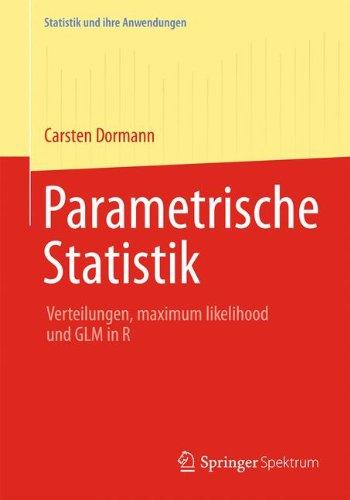
\includegraphics[width=2.08333in,height=\textheight]{./images/dormann.jpg}

}

\end{figure}

Dormann (2013) liefert ein tolles deutsches Buch für die Vertiefung in
die Statistik. Insbesondere wenn du wissenschaftlich Arbeiten willst
weit über die Bachelorarbeit hinaus. Dormann baut in seinem Buch eine
hervorragende Grundlage auf. Das Buch ist an der Hochschule Osnabrück
kostenlos
\href{https://link.springer.com/book/10.1007/978-3-662-54684-0}{über den
Link} zu erhalten.

\hypertarget{experimental-methods-in-agriculture}{%
\section{Experimental methods in
agriculture}\label{experimental-methods-in-agriculture}}

\begin{figure}

{\centering 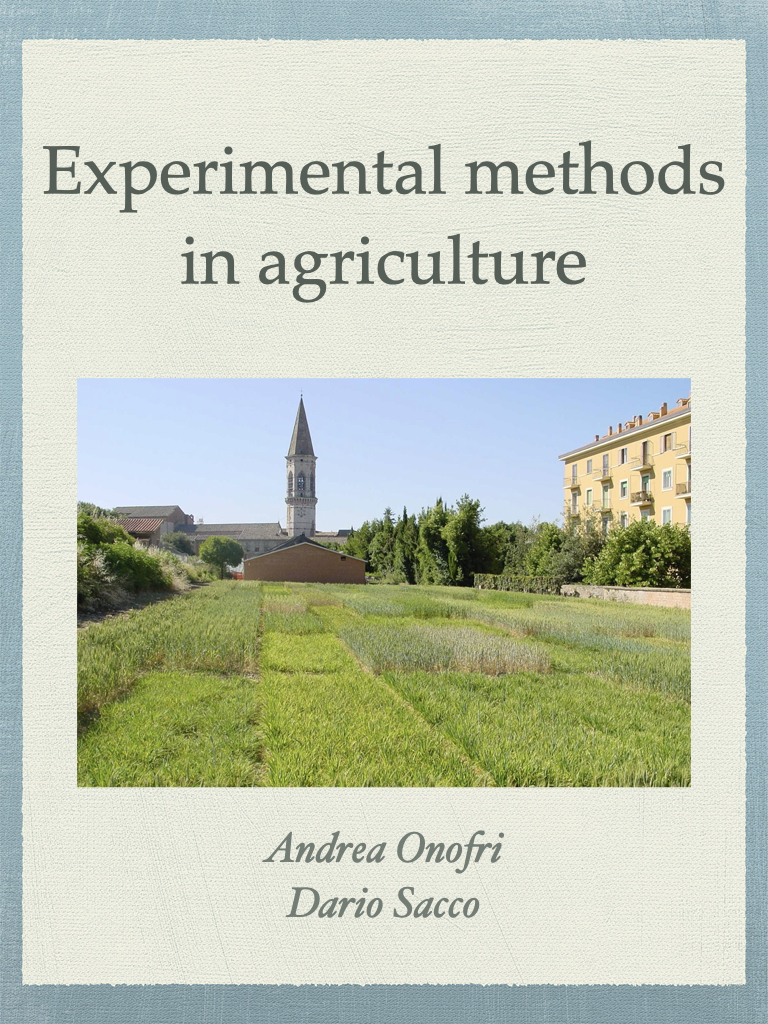
\includegraphics[width=2.08333in,height=\textheight]{./images/cover_stat_for_biology.jpeg}

}

\end{figure}

Onofri und Sacco (2021) haben das Buch
\href{https://www.statforbiology.com/_statbookeng/}{Experimental methods
in agriculture} geschrieben. Wir werden auf dieses englische Buch ab und
zu mal verweisen. Insbesondere der Einleitungstext zur Wissenschaft und
dem Design von Experiementen ist immer wieder lesenswert. Spätere Teile
des Buches sind etwas mathematischer und nicht für den Einstieg
unbedingt geeignet. Aber schaue es dir selber an.

\hypertarget{r-for-data-science}{%
\section{R for Data Science}\label{r-for-data-science}}

\begin{figure}

{\centering 
\includegraphics[width=2.08333in,height=\textheight]{./images/hadley.png}

}

\end{figure}

Wickham (2016) ist die Grundlage für die R Programmierung. Das Material
von Wickahm findet sich kostenlos online unter
\url{https://r4ds.had.co.nz/} und \url{https://www.tidyverse.org/}. Wir
werden uns hauptsächlich mit R wie es Wickham lehrt beschäftigen. Somit
ist Wickham unsere Grundlage für R.

\hypertarget{practical-statistics-for-data-scientists}{%
\section{Practical Statistics for Data
Scientists}\label{practical-statistics-for-data-scientists}}

\begin{figure}

{\centering 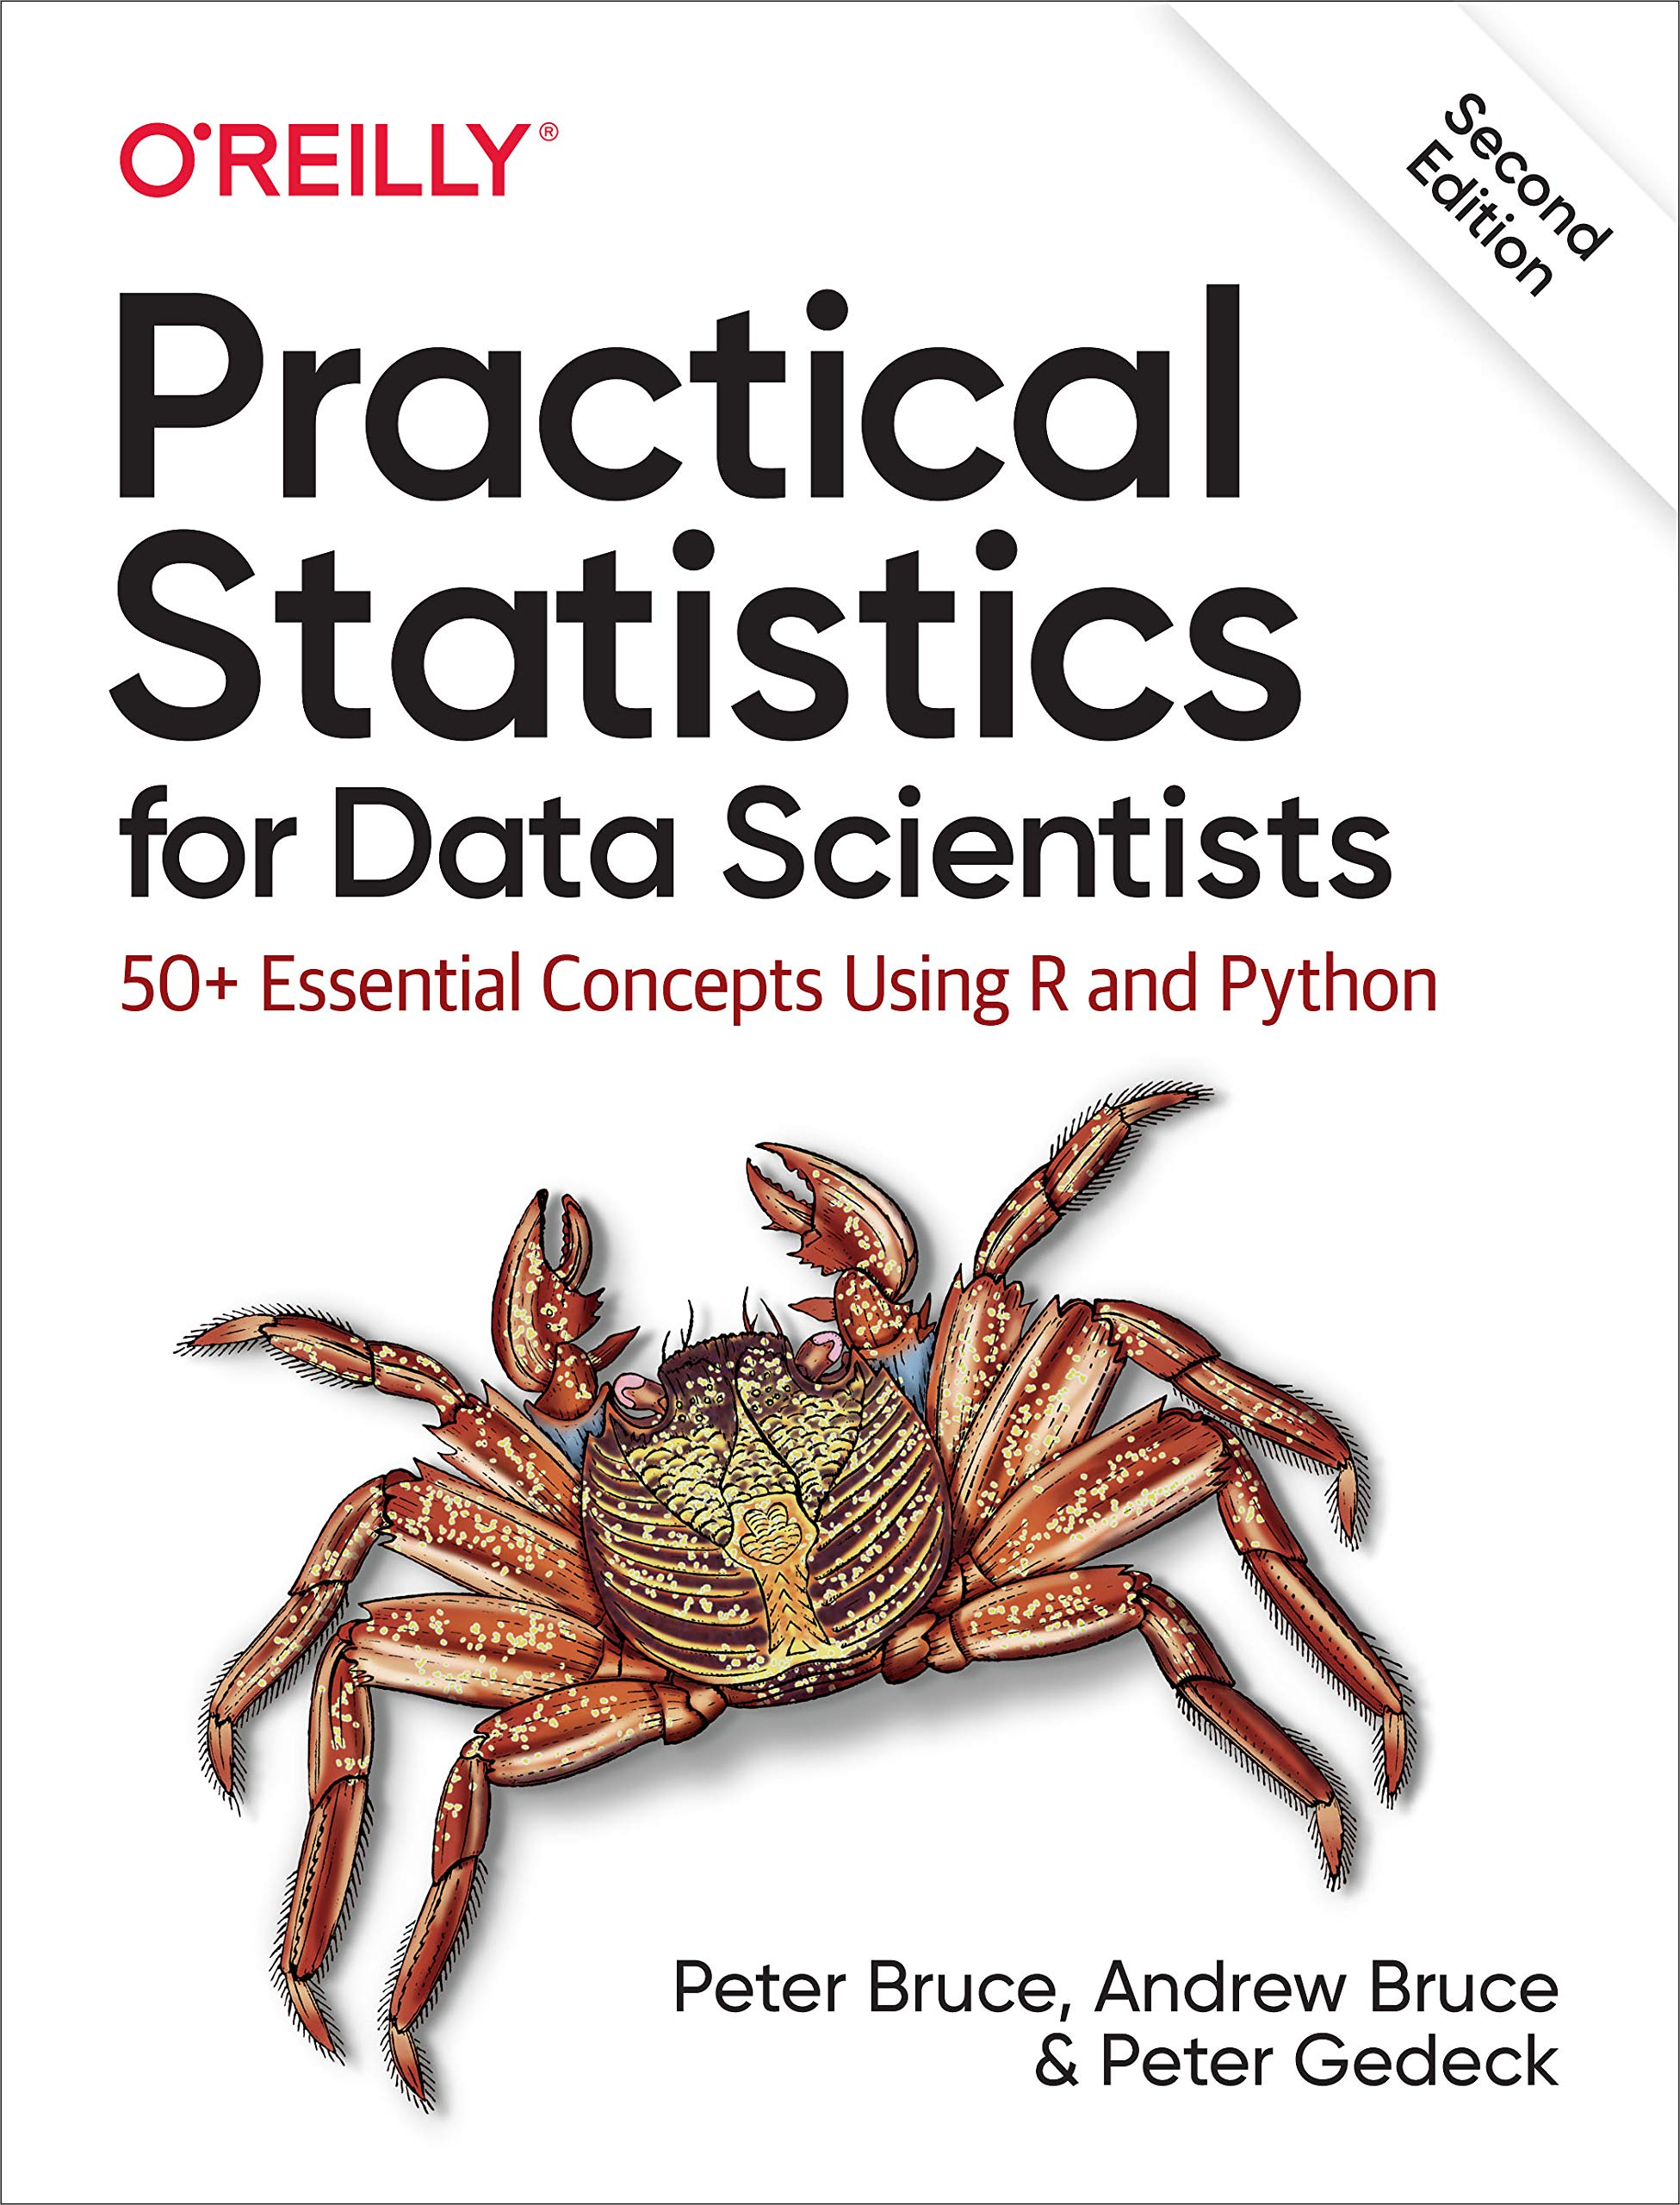
\includegraphics[width=2.08333in,height=\textheight]{./images/practical.jpg}

}

\end{figure}

Bruce (2020) schreibt ein Buch für den Anwender. Ohne Vorkenntnisse ist
das Buch vermutlich etwas schwer zu lesen. Dafür bietet das Buch aber
\emph{nach} einem Statistikkurs sehr gute Anknüpfungspunkte Richtung
maschinelles Lernen und somit der Klassifikation. Das Buch ist auch hier
in der
\href{https://ebookcentral.proquest.com/lib/hs-osnabrueck/detail.action?docID=6173908}{englischen
Version} und hier in der
\href{http://www.content-select.com/index.php?id=bib_view\&ean=9783960104674}{deutschen
Version} zu erhalten. \emph{Beide Links benötigen den Zugang über die
Hochschule Osnabrück}.

\hypertarget{data-science-for-agriculture-in-r}{%
\section{Data Science for Agriculture in
R}\label{data-science-for-agriculture-in-r}}

\begin{figure}

{\centering 
\includegraphics{./images/dsfair.png}

}

\end{figure}

Schmidt liefert auf der Webseite
\url{https://schmidtpaul.github.io/DSFAIR/index.html} eine tolle
Sammlung an experimentellen Designs bzw. Versuchsanlagen samt der
Auswertung in R. Ohne Vorkenntnisse schwer zu verstehen. Sollte aber
nach einem Kurs Statistik dann möglich sein. Gerne hier auch mich
fragen, dann können wir gemeinsam das passende Design raussuchen und
besprechen.

\hypertarget{odds-ends}{%
\section{Odds \& Ends}\label{odds-ends}}

\begin{figure}

{\centering 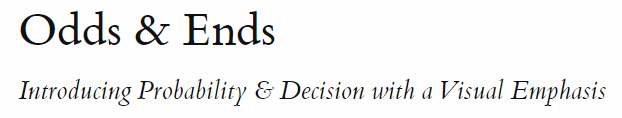
\includegraphics{./images/odds_and_ends.PNG}

}

\end{figure}

Am Ende dann noch eine Mathebuch von Weisberg zu finden unter
\url{https://jonathanweisberg.org/vip/}. Eigentlich eher ein Buch über
Wahrscheinlichkeiten und wenn ein Buch am Ende stehen muss, dann ist es
dieses Buch. Ich finde es sehr spannend zu lesen, aber das ist dann
vermutlich \emph{special intrest}.

\hypertarget{referenzen}{%
\section*{Referenzen}\label{referenzen}}
\addcontentsline{toc}{section}{Referenzen}

\bookmarksetup{startatroot}

\hypertarget{einfuxfchrung}{%
\chapter{Einführung}\label{einfuxfchrung}}

In diesem Kapitel nenne ich die wichtigsten Lernziele, die nach dem
Lesen des Skriptes von dir erreicht worden sein sollten. Je nach
besuchten Kurs kann natürlich nicht alles geschafft worden sein. So sehe
diese Übersicht als Einführung für das was später kommt. Wenn du die
Beispiele hir verstehst, dann hast du eine gute und solide Grundlage in
Statistik und Bio Data Science.

\hypertarget{ein-wort-der-warnung}{%
\section*{Ein Wort der Warnung\ldots{}}\label{ein-wort-der-warnung}}
\addcontentsline{toc}{section}{Ein Wort der Warnung\ldots{}}

Wenn du dieses Bild eines niedergeschlagenen \emph{Engels der Statistik}
siehst\ldots{}

\begin{figure}

{\centering 
\includegraphics[width=0.3\textwidth,height=\textheight]{./images/angel_01.png}

}

\end{figure}

\ldots{} dann bedeutet der niedergeschlagene Engel der Statistik:

\begin{enumerate}
\def\labelenumi{\arabic{enumi})}
\tightlist
\item
  Wir opfern Genauigkeit für Anwendbarkeit. Ja, manchmal ist es eben
  statstisch nicht richtig was hier steht, aber aus Gründen der
  Anwendung fahren wir mal über den Engel drüber. \emph{Schade}.
\item
  Wir sind hier Anfänger und Anwender. Später kannst du noch tiefer ins
  Detail gehen. Hier wollen wir die Grundlagen lernen. Das hat dann
  einen Preis an \emph{Richtigkeit}.
\item
  Wir wollen fertig werden. Durch geschicktes Manövrieren können wir an
  einen Punkt kommen, wo kein statistischer Test mehr passt. Das wollen
  wir nicht. Deshalb zahlen wir hier auch einen Preis. Passt aber.
\end{enumerate}

Deshalb konzentrieren wir uns auf einige wichtige Lernziele, die wir
jetzt einmal nacheinander durchgehen.

\hypertarget{lernziel-1-eine-explorative-datananalyse-durchfuxfchren}{%
\section{Lernziel 1: Eine explorative Datananalyse
durchführen}\label{lernziel-1-eine-explorative-datananalyse-durchfuxfchren}}

Gleich zu Beginn R Code zu zeigen und eine entsprechende Abbildung ist
vielleicht ungewöhnlich, aber wir wollen zu dieser
Abbildung~\ref{fig-boxplot-preface} hin. In
Abbildung~\ref{fig-boxplot-preface} siehst du einen Boxplot. Und wie wir
aus den Daten \texttt{flea\_dog\_cat.xlsx} einen Boxplot erstellen, das
soll uns in den nächsten Kapitel beschäftigen. Dafür müssen wir nämlich
eine Menge in dem Codeblock verstehen und dann auch Anwenden können. Und
natürlich lernen was eigentlich ein Boxplot ist und was in einem Boxplot
eigentlich dargestellt ist.

\href{https://github.com/jkruppa/jkruppa.github.io/blob/master/data/flea_dog_cat.xlsx}{Data}

\begin{figure}

{\centering 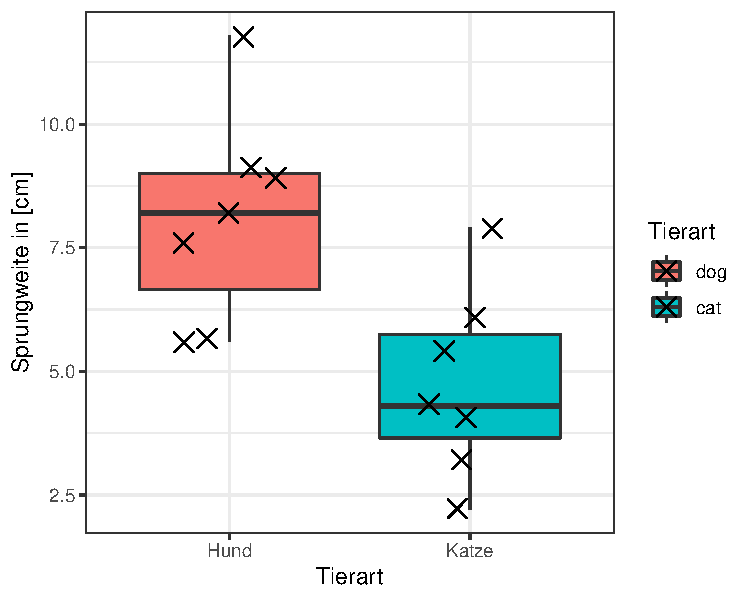
\includegraphics{./preface_files/figure-pdf/fig-boxplot-preface-1.pdf}

}

\caption{\label{fig-boxplot-preface}Boxplot der Sprungweiten {[}cm{]}
von Hunden und Katzen.}

\end{figure}

Hier ist der Codeblock der in R die Abbildung~\ref{fig-boxplot-preface}
erstellt.

\begin{Shaded}
\begin{Highlighting}[]
\DocumentationTok{\#\# Einlesen von Daten aus Excel}
\NormalTok{data\_tbl }\OtherTok{\textless{}{-}} \FunctionTok{read\_excel}\NormalTok{(}\StringTok{"data/flea\_dog\_cat.xlsx"}\NormalTok{)}

\DocumentationTok{\#\# Umformen der \textless{}chr\textgreater{} Spalte in einen Factor \textless{}fct\textgreater{}}
\NormalTok{data\_tbl }\OtherTok{\textless{}{-}}\NormalTok{ data\_tbl }\SpecialCharTok{\%\textgreater{}\%} 
  \FunctionTok{mutate}\NormalTok{(}\AttributeTok{animal =} \FunctionTok{as\_factor}\NormalTok{(animal))}

\DocumentationTok{\#\# Auswählen der wichtigen Spalten für den Boxplot}
\NormalTok{data\_tbl }\OtherTok{\textless{}{-}}\NormalTok{ data\_tbl }\SpecialCharTok{\%\textgreater{}\%} 
  \FunctionTok{select}\NormalTok{(animal, jump\_length) }

\DocumentationTok{\#\# Generieren des Boxplots in ggplot()}
\FunctionTok{ggplot}\NormalTok{(data\_tbl, }\FunctionTok{aes}\NormalTok{(}\AttributeTok{x =}\NormalTok{ animal, }\AttributeTok{y =}\NormalTok{ jump\_length, }
                     \AttributeTok{fill =}\NormalTok{ animal)) }\SpecialCharTok{+}
  \FunctionTok{geom\_boxplot}\NormalTok{() }\SpecialCharTok{+}
  \FunctionTok{geom\_jitter}\NormalTok{() }\SpecialCharTok{+}
  \FunctionTok{labs}\NormalTok{(}\AttributeTok{x =} \StringTok{"Tierart"}\NormalTok{, }\AttributeTok{y =} \StringTok{"Sprungweite in [cm]"}\NormalTok{, }
       \AttributeTok{fill =} \StringTok{"Tierart"}\NormalTok{) }\SpecialCharTok{+}
  \FunctionTok{scale\_x\_discrete}\NormalTok{(}\AttributeTok{labels =} \FunctionTok{c}\NormalTok{(}\StringTok{"Hund"}\NormalTok{, }\StringTok{"Katze"}\NormalTok{)) }\SpecialCharTok{+}
  \FunctionTok{theme\_bw}\NormalTok{()}
\end{Highlighting}
\end{Shaded}

Wir müssen nun folgende Dinge lernen um den Codeblock zu verstehen:

\begin{itemize}
\tightlist
\item
  Wir müssen das Datenbeispiel verstehen. Was sind das eigentlich für
  Daten, die wir da abbilden? Was sind überhaupt Daten im Sinne der
  Statistik bzw. für R.
\item
  Wir müssen den R Code verstehen. Von einzelnen wichtigen Opertatoren
  wie \texttt{-\textgreater{}} und
  \texttt{\%\textbackslash{}\textgreater{}\%} zu dem den Unterschieden
  von Worten und Objekten.
\item
  Wie kriegen wir Daten aus Excel in R hinein? Wir können die Daten ja
  nicht einfach in R eintragen sondern haben die Daten ja meist in einer
  (Excel) Datei wie \texttt{flea\_dog\_cat.xlsx}.
\item
  Was ist eigentlich ein Boxplot und welche statistsichen Maßzahlen
  werden hier eigentlich abgebildet?
\item
  Wie funktioniert eigentlich die Funktioen \texttt{ggplot()} mit der
  wir den Boxplot erstellt haben?
\end{itemize}

All diese Fragen und weitere Fragen, die sich diesen Fragen anschließen,
wollen wir uns in den nächsten Kapitel anschauen. Leider kann ich hier
nur \emph{linear} schreiben. Deshalb musst du eventuell mal ein Kapitel
wiederholen oder etwas quer lesen. Du kanst dir ja auch nicht immer
alles auf einmal merken.

\hypertarget{lernziel-2-rstudio-und-r}{%
\section{Lernziel 2: RStudio und R}\label{lernziel-2-rstudio-und-r}}

Um Data Science durchführen zu können musst du etwas Programmieren
können. Wir programmieren in R und nutzen die Software um Abbildungen zu
erstellen und Analysen zu rechnen.

Wir arbeiten in R und nutzen dafür das RStudio. Führe einfach folgende
Schritte aus um erst R zu installieren und dann das RStudio.

\begin{enumerate}
\def\labelenumi{\arabic{enumi}.}
\tightlist
\item
  R installieren unter \url{https://cran.rstudio.com/}
\item
  RStudio installieren unter
  \url{https://www.rstudio.com/products/rstudio/download/\#download}
\end{enumerate}

Bitte die Reihenfolge beachten. Beide Schritte kannst du dir auch
nochmals im Video anschauen oder aber du kommst in das R Tutorium was
regelmäßig an der Hochschule Osnabrück von mir angeboten wird. Die
Termine findest du im Kapitel~\ref{sec-r-tutorium}.

\begin{tcolorbox}[enhanced jigsaw, bottomrule=.15mm, toptitle=1mm, colbacktitle=quarto-callout-tip-color!10!white, opacityback=0, bottomtitle=1mm, leftrule=.75mm, toprule=.15mm, breakable, rightrule=.15mm, title=\textcolor{quarto-callout-tip-color}{\faLightbulb}\hspace{0.5em}{Was ist eigentlich RStudio und woher kriege ich das?}, coltitle=black, colframe=quarto-callout-tip-color-frame, colback=white, titlerule=0mm, left=2mm, arc=.35mm, opacitybacktitle=0.6]
Du findest auf YouTube \href{https://youtu.be/krF7TJVb-UA}{Einführung in
R - Teil 01 - Installation von RStudio und R} als Video. Ich gehe in dem
Video einmal alle wichtigen Schritte durch und so kannst du dir Rstudio
und R installieren.
\end{tcolorbox}

\hypertarget{lernziel-3-statistische-versuche-verstehen}{%
\section{Lernziel 3: Statistische Versuche
verstehen}\label{lernziel-3-statistische-versuche-verstehen}}

Wie funktioniert ein \emph{statistischer} Versuch? Ich könnte auch
wissenschaftliches Experiment schreiben, aber ein wissenschaftliches
Experiment ist sehr abstrakt. Wir wollen ja einen Versuch durchführen
und danach - ja was eigentlich? Was wollen wir nach dem Versuch haben?
Meistens eine neue Erkenntnis. Um diese Erkenntnis zu validieren oder
aber abzusichern nutzen wir Statistik. Dazu musst du noch wissen, dass
wir eine spezielle Form der Statistik nutzen: die \emph{frequentistische
Statistik}.

{\marginnote{\begin{footnotesize}Eine \textbf{biologische Wiederholung}
beinhaltet ein neues Tier, Pflanze oder Mensch. Eine \textbf{technische}
Wiederholung ist die gleiche Messung an dem gleichen Tier, Pflanze oder
Mensch.\end{footnotesize}}}

{\marginnote{\begin{footnotesize}Wir nennen das \textbf{Outcome} auch
\textbf{Endpunkt}, \textbf{Response} oder kurz
\(y\).\end{footnotesize}}}

Die \emph{frequentistische Statistik} basiert - wie der Name andeutet -
auf Wiederholungen in einem Versuch. Daher der Name frequentistisch.
Also eine Frequenz von Beobachtungen. Ist ein wenig gewollt, aber daran
gewöhnen wir uns schon mal. Konkret, ein Experiment welches wir
frequentistisch Auswerten wollen besteht immer aus biologischen
Wiederholungen. Wir müssen also ein Experiment planen in dem wir
wiederholt ein Outcome an vielen Tieren, Pflanzen oder Menschen messen.
Auf das Outcome gehen wir noch später ein. Im Weiteren konzentrieren wir
uns hier auf die \emph{parametrische} Statistik. Die parametrische
Statistik beschäftigt sich mit Parametern von Verteilungen. Ein
schwieriger Satz. Schauen wir uns einmal eine Verteilung an.

\hypertarget{possionverteilung}{%
\subsection{Possionverteilung}\label{possionverteilung}}

Abbildung~\ref{fig-preface-pois-1} zeigt eine Poissonverteilung. Eine
Poissonverteilung beschreibt Zähldaten. Mehr zu der Poissonverteilung
findest du im Kapitel~\ref{sec-poisson}. Wir zählen bei 39 Hunden
wiviele Flöhe jeder Hund jeweils hatte. Danach zeichnen wir uns einen
Dotplot der die Verteilung der Anzahl Flöhe auf den Hunden
wiederspiegelt.

\begin{figure}

{\centering 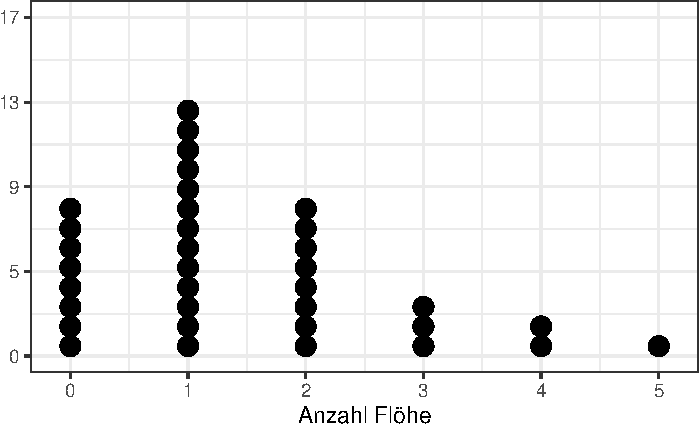
\includegraphics{./preface_files/figure-pdf/fig-preface-pois-1-1.pdf}

}

\caption{\label{fig-preface-pois-1}An 39 Hunden wurde die Anzahl an
Flöhen gezählt.}

\end{figure}

{\marginnote{\begin{footnotesize}\textbf{Parameter} sind Zahlen, die
eine Verteilungskurve beschreiben.\end{footnotesize}}}

Eine Verteilung hat Parameter. Parameter sind die Eigenschaften einer
Verteilung, die notwendig sind um eine Verteilung vollständig zu
beschreiben.

Im Falle der Possionverteilung brauchen wir nur einen Paramter für den
höchsten Punkt der Kurve. Wir nennen diesen Punkt \emph{Lambda}
(\(\lambda\)). Die Ausbreitung der Kurve ist eine Funktion von
\(\lambda\) und steigt mit \(\lambda\) an.

\hypertarget{normalverteilung}{%
\subsection{Normalverteilung}\label{normalverteilung}}

Abbildung~\ref{fig-preface-normal-1} zeigt eine Normalverteilung. Mehr
zu der Poissonverteilung findest du im Kapitel~\ref{sec-normal}. Hier
haben wir das Flohgewicht von den Flöhen von 24 Hunden gemessen, die mit
Flöhen befallen waren. Wir sehen, dass sich eine Glockenkurve bildet
oder zumindestens etwas ähnliches. Wir können annehmen, dass das Gewicht
\emph{approximativ} normalverteilt ist.

{\marginnote{\begin{footnotesize}Wir nutzen das Wort
\textbf{approximativ} wenn wir sagen wollen, dass ein Outcome
näherungsweise normalverteilt ist.\end{footnotesize}}}

\begin{figure}

{\centering 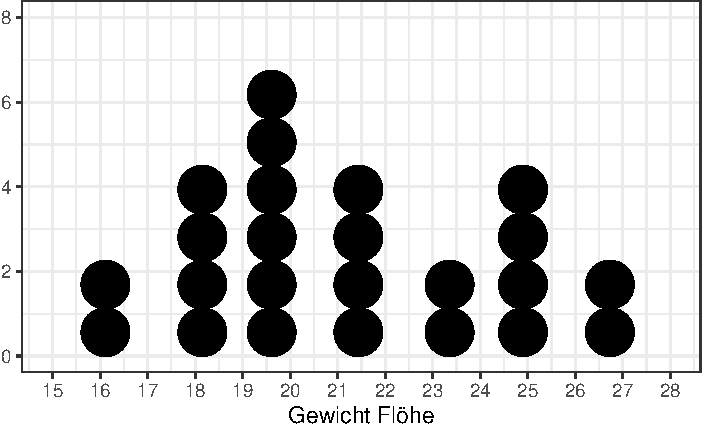
\includegraphics{./preface_files/figure-pdf/fig-preface-normal-1-1.pdf}

}

\caption{\label{fig-preface-normal-1}An 39 Hunden wurde die Anzahl an
Flöhen gezählt.}

\end{figure}

Im Falle der Normalverteilung brauchen wir einen Paramter für den
höchsten Punkt der Kurve, sowie einen Parameter für die Ausbreitung,
also wie weit geht die Kurve nach links und nach rechts. Der Mittelwert
\(\bar{y}\) beschriebt den höchsten Punkt einer Normalverteilung. Die
Standardabweichung \(s_y\) beschreibt die Ausbreitung einer
Normalverteilung.

\begin{tcolorbox}[enhanced jigsaw, bottomrule=.15mm, toptitle=1mm, colbacktitle=quarto-callout-note-color!10!white, opacityback=0, bottomtitle=1mm, leftrule=.75mm, toprule=.15mm, breakable, rightrule=.15mm, title=\textcolor{quarto-callout-note-color}{\faInfo}\hspace{0.5em}{Wie gehen wir nun vor, wenn wir ein Experiment durchführen wollen?}, coltitle=black, colframe=quarto-callout-note-color-frame, colback=white, titlerule=0mm, left=2mm, arc=.35mm, opacitybacktitle=0.6]

\begin{enumerate}
\def\labelenumi{\arabic{enumi})}
\tightlist
\item
  Wir müssen auf jeden Fall wiederholt ein Outcome an verschiedenen
  Tieren, Pflanzen oder Menschen messen.
\item
  Wir überlegen uns aus welcher Verteilungsfamilie unser Outcome stammt,
  damit wir dann die entsprechende Verfahren zur Analyse nehmen können.
\end{enumerate}

\end{tcolorbox}

\hypertarget{lernziel-4-falsifikationsprinzip}{%
\section{Lernziel 4:
Falsifikationsprinzip}\label{lernziel-4-falsifikationsprinzip}}

\begin{tcolorbox}[enhanced jigsaw, bottomrule=.15mm, toptitle=1mm, colbacktitle=quarto-callout-tip-color!10!white, opacityback=0, bottomtitle=1mm, leftrule=.75mm, toprule=.15mm, breakable, rightrule=.15mm, title=\textcolor{quarto-callout-tip-color}{\faLightbulb}\hspace{0.5em}{Grundlagen der Wissenschaft und Falsifikationsprinzip}, coltitle=black, colframe=quarto-callout-tip-color-frame, colback=white, titlerule=0mm, left=2mm, arc=.35mm, opacitybacktitle=0.6]
Du findest auf YouTube \href{https://youtu.be/h45ftLNsspM}{Grundlagen
der Wissenschaft und Falsifikationsprinzip} als Video Reihe.
\end{tcolorbox}

Wenn wir ein Experiment durchführen dann erheben wir einmalig Daten
\(D_1\). Wir könnten das Experiment wiederholen und erneut Daten \(D_2\)
erheben. Wir können das Experiment \(j\)-mal wiederholen und haben dann
Daten von \(D_1,..., D_j\). Dennoch werden wir nie \emph{alle} Daten
erheben können, die mit einem Experiment verbunden sind.

{\marginnote{\begin{footnotesize}\textbf{Strukturgleichkeit} erreichen
wir durch \textbf{Randomisierung}.\end{footnotesize}}}

Nehmen wir das Beispiel, dass wir die Sprungweite von Hunde- und
Katzenflöhen vergleichen wollen. Wir können nicht \emph{alle} Hunde- und
Katzenflöhe messen. Wir können nur eine Stichprobe an Daten \(D_1\)
erheben. Über diese Daten \(D_1\) können wir dann später durch
statistische Algorithmen eine Aussage treffen. Wichtig ist hier sich zu
merken, dass wir eine Grundgesamtheit haben aus der wir eine Stichprobe
ziehen. Wir müssen darauf achten, dass die Stichprobe
\emph{repräsentativ} ist und damit \emph{strukturgleich} zur
Grundgesamtheit ist. Die Strukturgleichkeit erreichen wir durch
Randomisierung. Wir veranschaulichen diesen Zusammenhang in
Abbildung~\ref{fig-grundgesamtheit-schema}. Ein Rückschluß von der
Stichprobe ist nur möglich, wenn die Stichprobe die Grundgesamtheit
repräsentiert. Auch eine Randomisierung mag dieses Ziel nicht immer
erreichen. Im Beispiel der Hundeflöhe könnte wir eine Art an Flöhen
übersehen und diese Flohart nicht mit in die Stichprobe aufnehmen. Ein
Rückschluß auf diese Flohart wäre dann mit unserem Experiment nicht
möglich.

\begin{figure}

{\centering 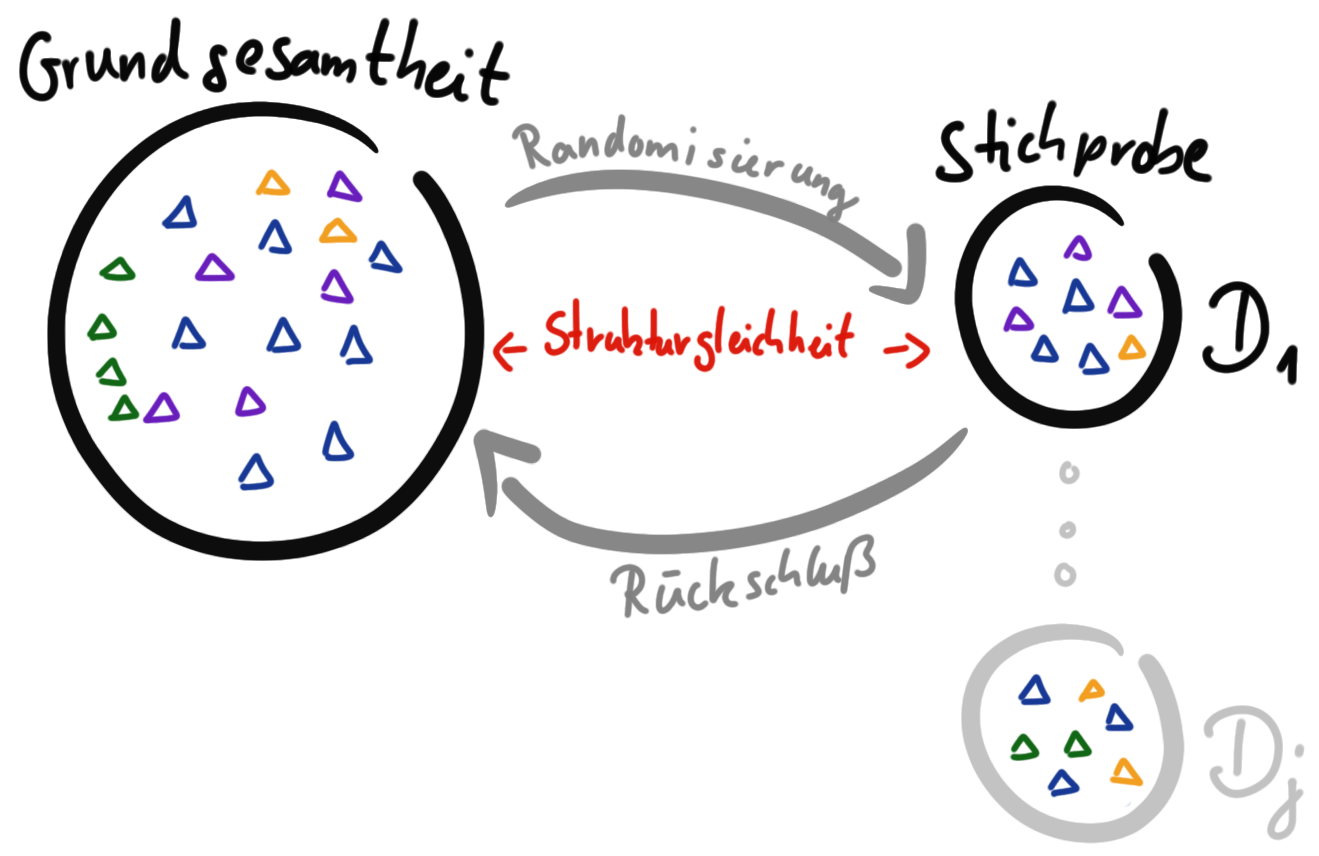
\includegraphics[width=0.8\textwidth,height=\textheight]{./images/preface-grundgesamtheit.png}

}

\caption{\label{fig-grundgesamtheit-schema}Abbildung über die
Grundgesamtheit und die Stichprobe(n) \(D_1\) bis \(D_j\). Durch
Randomisierung wird Sturkturgleichheit erreicht, die dann einen
Rückschluß von der Stichprobe auf die Grundgesamtheit erlaubt. Jede
Stichprobe ist anders und nicht jede Randomisierung ist erfolgreich was
die Strukturgleicheit betrifft.}

\end{figure}

Tabelle~\ref{tbl-grundgesamtheit-stichprobe} zeigt nochmal die
Zusammenfassung von der Grundgesamtheit un der Stichprobe im Vergleich.
Wichtig ist zu merken, dass wir mit unserem kleinen Experiment Daten
\(D\) generieren mit denen wir einen Rückschluß und somit eine
Verallgemeinerung erreichen wollen.

\hypertarget{tbl-grundgesamtheit-stichprobe}{}
\begin{longtable}[]{@{}
  >{\raggedright\arraybackslash}p{(\columnwidth - 2\tabcolsep) * \real{0.5221}}
  >{\raggedright\arraybackslash}p{(\columnwidth - 2\tabcolsep) * \real{0.4779}}@{}}
\caption{\label{tbl-grundgesamtheit-stichprobe}Vergleich von
Grundgesamtheit und Stichprobe.}\tabularnewline
\toprule()
\begin{minipage}[b]{\linewidth}\raggedright
Grundgesamtheit
\end{minipage} & \begin{minipage}[b]{\linewidth}\raggedright
Stichprobe
\end{minipage} \\
\midrule()
\endfirsthead
\toprule()
\begin{minipage}[b]{\linewidth}\raggedright
Grundgesamtheit
\end{minipage} & \begin{minipage}[b]{\linewidth}\raggedright
Stichprobe
\end{minipage} \\
\midrule()
\endhead
\ldots{} \(n\) ist riesig bis unfassbar. & \ldots{} \(n\) von \(D\) ist
klein. \\
\ldots{} der Mittelwert wird mit \(\mu_y\) beschrieben. & \ldots{} der
Mittelwert wird mit \(\bar{y}\) beschrieben. \\
\ldots{} die Varianz wird mit \(\sigma^2\) beschrieben. & \ldots{} die
Varianz wird mit \(s^2\) beschrieben. \\
\ldots{} die Standardabweichung wird mit \(\sigma\) beschrieben. &
\ldots{} die Standardabweichung wird mit \(s\) beschrieben. \\
\bottomrule()
\end{longtable}

\part{Datenbeispiele}

Wir brauchen am Anfang erstmal ein simples Beispiel. Konkrete Zahlen mit
denen wir arbeiten können und Grundlagen aufbauen können. Was liegt da
näher als sich einmal am Kopf zu kratzen und zu fragen, was juckt den
da? Genau! Flöhe. Wir schauen uns einmal Flöhe auf Hunden und Katzen an.
Daran können wir viel über Zahlen und Buchstaben in der Statistik und
dann im Programmieren lernen.

\begin{tcolorbox}[enhanced jigsaw, bottomrule=.15mm, toptitle=1mm, colbacktitle=quarto-callout-note-color!10!white, opacityback=0, bottomtitle=1mm, leftrule=.75mm, toprule=.15mm, breakable, rightrule=.15mm, title=\textcolor{quarto-callout-note-color}{\faInfo}\hspace{0.5em}{Zahlen, Buchstaben und Wörter}, coltitle=black, colframe=quarto-callout-note-color-frame, colback=white, titlerule=0mm, left=2mm, arc=.35mm, opacitybacktitle=0.6]
Mir ist bewusst, dass du die Unterschiede kennst. Nur leider ist eine
Zahl nicht nur eine Zahl und ein Wort nicht immer ein Wort. Das hat mit
der eingeschränkten Kommunikationsfähigkeit von Computerprogrammen zu
tun. R braucht da deine Mithilfe und dein \emph{neues} Verständnis von
Buchstaben und Zahlen. Eben wie ein Computer denkt.
\end{tcolorbox}

\hypertarget{von-fluxf6hen-und-hunden}{%
\section*{Von Flöhen und Hunden}\label{von-fluxf6hen-und-hunden}}
\addcontentsline{toc}{section}{Von Flöhen und Hunden}

In unserem ersten Beispiel in Kapitel~\ref{sec-example-1} geht es darum
einmal ein Gefühl für Daten zu kriegen. Also was sind diese Zahlen und
Buchstaben eigentlich? Wie sind Daten aufgebaut und wie musst du Daten
bauen, so dass wir auch mit den Daten arbeiten können? Wir schauen uns
dafür einmal Flöhe auf Hunden an und fragen uns welche Typen von Zahlen
können wir erheben?

\hypertarget{von-fluxf6hen-hunden-und-katzen}{%
\section*{Von Flöhen, Hunden und
Katzen}\label{von-fluxf6hen-hunden-und-katzen}}
\addcontentsline{toc}{section}{Von Flöhen, Hunden und Katzen}

In unserem zweiten Beispiel in Kapitel~\ref{sec-example-2} erweitern wir
unserer erstes Beispiel aus Kapitel~\ref{sec-example-1} um die Katzen.
Das heist, dass eigentlich alles gleich bleibt. Wir schauen usn
\emph{zusätlich} noch als zweite Gruppe die Katzen an. Nun können wir
die Frage stellen, unterscheiden sich Flöhe auf Hunden und Katzen
gegeben von gemessenen Eigenschaften?

\hypertarget{von-fluxf6hen-auf-tieren}{%
\section*{Von Flöhen auf Tieren}\label{von-fluxf6hen-auf-tieren}}
\addcontentsline{toc}{section}{Von Flöhen auf Tieren}

In unserem dritten Beispiel in Kapitel~\ref{sec-example-3} erweitern wir
das Beispiel um den Fuchs mit einem weiteren Tier. Dadurch haben wir
nicht mehr einen Faktor mit zwei Leveln vorliegen sondern einen mit drei
Leveln. Die Fragestrellung erweitert sich jetzt auf einen
\emph{multiplen} Gruppenvergleich. Wir vergleichen nicht mehr nur noch
zwei Gruppen miteinander sondern drei.

\hypertarget{von-fluxf6hen-auf-tieren-in-habitaten}{%
\section*{Von Flöhen auf Tieren in
Habitaten}\label{von-fluxf6hen-auf-tieren-in-habitaten}}
\addcontentsline{toc}{section}{Von Flöhen auf Tieren in Habitaten}

In unserem vierten Beispiel in Kapitel~\ref{sec-example-4} schauen wir
uns zusätzlich zu dem dritten Beispiel in Kapitel~\ref{sec-example-3}
noch verschiedene Habitate (eng. \emph{site}) an. Wir haben nämlich die
Hunde-, Katzen-, und Fuchsflöhe nicht nur an einem Ort sondern an
verschiedenen Orten gesammelt und gemessen. Wir haben einen zweiten
Faktor vorliegen.

\hypertarget{sec-example-1}{%
\chapter{Von Flöhen und Hunden}\label{sec-example-1}}

In unserem ersten Beispiel wollen wir uns verschiedene Daten \(D\) von
Hunden und Hundeflöhen anschauen. Unter anderem sind dies die
Sprungweite, die Anzahl an Flöhen, die Boniturnoten auf einer Hundemesse
sowie der Infektionsstatus. Hier nochmal detailiert, was wir uns im
folgenden im Kapitel einmal anschauen wollen.

\begin{itemize}
\item
  \textbf{Sprungweite} in {[}cm{]} von verschiedenen Flöhen \[
  Y_{jump} = \{5.7, 8.9, 11.8, 8.2, 5.6, 9.1, 7.6\}.
  \]
\item
  \textbf{Anzahl an Flöhen} auf verschiedenen Hunden \[
    Y_{count} = \{18, 22, 17, 12, 23, 18, 21\}.
    \]
\item
  \textbf{Boniturnoten} {[}1 = schlechteste bis 9 = beste Note{]} von
  verschiedenen Hunden \[
    Y_{grade} = \{8, 8, 6, 8, 7, 7, 9\}.
    \]
\item
  \textbf{Infektionstatus} {[}0 = gesund, 1 = infiziert{]} mit Flöhen
  von verschiedenen Hunden \[
    Y_{infected} = \{0, 1, 1, 0, 1, 0, 0\}.
    \]
\end{itemize}

Je nachdem was wir messen, nimmt \(Y\) andere Zahlenräume an. Wir sagen,
\(Y\) folgt einer Verteilung. Die Sprungweite ist normalverteilt, die
Anzahl an Flöhen folgt einer Poisson Verteilung, die Boniturnoten sind
multinominal/ordinal bzw. kategorial verteilt. Der Infektionsstatus ist
binomial verteilt. Wir werden uns später die Verteilungen anschauen und
visualisieren. Das können wir hier aber noch nicht. Wichtig ist, dass du
schon mal gehört hast, dass \(Y\) unterschiedlich \emph{verteilt} ist,
je nachdem welche Dinge wir messen.

Tabelle~\ref{tbl-dog-long} zeigt dir die Darstellung der Daten von oben
in einer einzigen Tabelle. Bitte bachte, dass genau eine Zeile für eine
Beobachutng, in diesem Fall einem Hund, vorgesehen ist.

\hypertarget{tbl-dog-long}{}
\begin{longtable}[]{@{}ccccc@{}}
\caption{\label{tbl-dog-long}Sprunglängen {[}cm{]} für Hundeflöhe. Die
Tabelle ist im Long-Format dargestellt.}\tabularnewline
\toprule()
animal & jump\_length & flea\_count & grade & infected \\
\midrule()
\endfirsthead
\toprule()
animal & jump\_length & flea\_count & grade & infected \\
\midrule()
\endhead
dog & 5.7 & 18 & 8 & 0 \\
dog & 8.9 & 22 & 8 & 1 \\
dog & 11.8 & 17 & 6 & 1 \\
dog & 8.2 & 12 & 8 & 0 \\
dog & 5.6 & 23 & 7 & 1 \\
dog & 9.1 & 18 & 7 & 0 \\
dog & 7.6 & 21 & 9 & 0 \\
\bottomrule()
\end{longtable}

\begin{tcolorbox}[enhanced jigsaw, bottomrule=.15mm, toptitle=1mm, colbacktitle=quarto-callout-tip-color!10!white, opacityback=0, bottomtitle=1mm, leftrule=.75mm, toprule=.15mm, breakable, rightrule=.15mm, title=\textcolor{quarto-callout-tip-color}{\faLightbulb}\hspace{0.5em}{Datei für von Flöhen und Hunden}, coltitle=black, colframe=quarto-callout-tip-color-frame, colback=white, titlerule=0mm, left=2mm, arc=.35mm, opacitybacktitle=0.6]
Du findest die Datei \texttt{flea\_dog.xlsx} auf GitHub
\href{https://github.com/jkruppa/jkruppa.github.io/tree/master/data}{jkruppa.github.io/data/}
als Excel oder auch als CSV.
\end{tcolorbox}

\hypertarget{sec-example-2}{%
\chapter{Von Flöhen, Hunden und Katzen}\label{sec-example-2}}

Wir wollen jetzt das Beispiel von den Hunden und Flöhen um eine Spezies
erweitern. Wir nehmen noch die Katzen mit dazu und fragen uns, wie sieht
es mit der Sprungfähigkeit von Katzen und Hundeflöhen aus? Konzentrieren
wir uns hier einmal auf die Sprungweite. Wir können wie in dem Beispiel
\ref{sec-example-1} die Sprungweiten {[}cm{]} wieder aufschreiben:

\[
Y_{jump} = \{3.2, 2.2, 5.4, 4.1, 4.3, 7.9, 6.1\}.
\]

Wenn wir jetzt die Sprungweiten der Hundeflöhe mit den Katzenflöhen
vergleichen wollen haben wir ein Problem. Beide Zahlenvektoren heißen
gleich, nämlich \(Y_{jump}\). Wir könnten jeweils in die Indizes noch
\(dog\) und \(cat\) schreiben als \(Y_{jump,\, dog}\) und
\(Y_{jump,\, cat}\) und erhalten folgende Vektoren.

\[
Y_{jump,\, dog} = \{5.7, 8.9, 11.8, 8.2, 5.6, 9.1, 7.6\}
\]

\[
Y_{jump,\, cat} = \{3.2, 2.2, 5.4, 4.1, 4.3, 7.9, 6.1\}
\]

Dadurch werden die Indizes immer länger und unübersichticher. Auch das
\(Y\) einfach \(Y_{dog}\) oder \(Y_{cat}\) zu nennen ist keine Lösung -
wir wollen uns vielleicht später nicht nur die Sprungweite vergleichen,
sondern vielleicht auch die Anzahl an Flöhen oder den Infektionsstatus.
Dann ständen wir wieder vor dem Problem die \(Y\) für die verschiedenen
Outcomes zu unterscheiden. Daher erstellen wir uns die
Tabelle~\ref{tbl-dog-cat-wide}. Wir haben jetzte eine
\emph{Daten}tabelle.

\hypertarget{tbl-dog-cat-wide}{}
\begin{longtable}[]{@{}cc@{}}
\caption{\label{tbl-dog-cat-wide}Sprunglängen {[}cm{]} für Hunde- und
Katzenflöhe. Die Tabelle ist im Wide-Format dargestellt.}\tabularnewline
\toprule()
dog & cat \\
\midrule()
\endfirsthead
\toprule()
dog & cat \\
\midrule()
\endhead
5.7 & 3.2 \\
8.9 & 2.2 \\
11.8 & 5.4 \\
8.2 & 4.1 \\
5.6 & 4.3 \\
9.1 & 7.9 \\
7.6 & 6.1 \\
\bottomrule()
\end{longtable}

Intuitiv ist die Tabelle~\ref{tbl-dog-cat-wide} übersichtlich und
beinhaltet die Informationen die wir wollten. Dennoch haben wir das
Probem, das wir in dieser Tabelle~\ref{tbl-dog-cat-wide} nicht noch
weitere Outcomes angeben können. Wir können die Anzahl an Flöhen auf den
Hunde und Katzen nicht darstellen. Als Lösung ändern wir die
Tabelle~\ref{tbl-dog-cat-wide} in das Long-Format. Dargestellt in
Tabelle~\ref{tbl-dog-cat-long}. Jede Beobachtung belegt nun eine Zeile.
Dies ist sehr wichtig im Kopf zu behalten, wenn du eigene Daten in z.B.
Excel eingibts.

\hypertarget{tbl-dog-cat-long}{}
\begin{longtable}[]{@{}ccccc@{}}
\caption{\label{tbl-dog-cat-long}Tabelle der Sprunglängen {[}cm{]},
Anzahl an Flöhen, Boniturnote sowie der Infektionsstatus von Hunde- und
Katzenflöhe. Die Tabelle ist im Long-Format dargestellt.}\tabularnewline
\toprule()
animal & jump\_length & flea\_count & grade & infected \\
\midrule()
\endfirsthead
\toprule()
animal & jump\_length & flea\_count & grade & infected \\
\midrule()
\endhead
dog & 5.7 & 18 & 8 & 0 \\
dog & 8.9 & 22 & 8 & 1 \\
dog & 11.8 & 17 & 6 & 1 \\
dog & 8.2 & 12 & 8 & 0 \\
dog & 5.6 & 23 & 7 & 1 \\
dog & 9.1 & 18 & 7 & 0 \\
dog & 7.6 & 21 & 9 & 0 \\
cat & 3.2 & 12 & 7 & 1 \\
cat & 2.2 & 13 & 5 & 0 \\
cat & 5.4 & 11 & 7 & 0 \\
cat & 4.1 & 12 & 6 & 0 \\
cat & 4.3 & 16 & 6 & 1 \\
cat & 7.9 & 9 & 6 & 0 \\
cat & 6.1 & 7 & 5 & 0 \\
\bottomrule()
\end{longtable}

\begin{tcolorbox}[enhanced jigsaw, bottomrule=.15mm, toptitle=1mm, colbacktitle=quarto-callout-tip-color!10!white, opacityback=0, bottomtitle=1mm, leftrule=.75mm, toprule=.15mm, breakable, rightrule=.15mm, title=\textcolor{quarto-callout-tip-color}{\faLightbulb}\hspace{0.5em}{Datei für von Flöhen, Hunden und Katzen}, coltitle=black, colframe=quarto-callout-tip-color-frame, colback=white, titlerule=0mm, left=2mm, arc=.35mm, opacitybacktitle=0.6]
Du findest die Datei \texttt{flea\_dog\_cat.xlsx} auf GitHub
\href{https://github.com/jkruppa/jkruppa.github.io/tree/master/data}{jkruppa.github.io/data/}
als Excel oder auch als CSV.
\end{tcolorbox}

\hypertarget{sec-example-3}{%
\chapter{Von Flöhen auf Tieren}\label{sec-example-3}}

Wir wollen jetzt das Beispiel von den Hunde- und Katzenflöhen um eine
\emph{weitere} Spezies erweitern. Wir nehmen noch die Füchse mit dazu
und fragen uns, wie sieht es mit der Sprungfähigkeit von Hunde-, Katzen-
und Fuchsflöhen aus?

\hypertarget{tbl-dog-cat-fox}{}
\begin{longtable}[]{@{}ccccc@{}}
\caption{\label{tbl-dog-cat-fox}Sprunglängen {[}cm{]} für Hunde-,
Katzen- und Fuchsflöhe.}\tabularnewline
\toprule()
animal & jump\_length & flea\_count & grade & infected \\
\midrule()
\endfirsthead
\toprule()
animal & jump\_length & flea\_count & grade & infected \\
\midrule()
\endhead
dog & 5.7 & 18 & 8 & 0 \\
dog & 8.9 & 22 & 8 & 1 \\
dog & 11.8 & 17 & 6 & 1 \\
dog & 8.2 & 12 & 8 & 0 \\
dog & 5.6 & 23 & 7 & 1 \\
dog & 9.1 & 18 & 7 & 0 \\
dog & 7.6 & 21 & 9 & 0 \\
cat & 3.2 & 12 & 7 & 1 \\
cat & 2.2 & 13 & 5 & 0 \\
cat & 5.4 & 11 & 7 & 0 \\
cat & 4.1 & 12 & 6 & 0 \\
cat & 4.3 & 16 & 6 & 1 \\
cat & 7.9 & 9 & 6 & 0 \\
cat & 6.1 & 7 & 5 & 0 \\
fox & 7.7 & 21 & 5 & 1 \\
fox & 8.1 & 25 & 4 & 1 \\
fox & 9.1 & 31 & 4 & 1 \\
fox & 9.7 & 12 & 5 & 1 \\
fox & 10.6 & 28 & 4 & 0 \\
fox & 8.6 & 18 & 4 & 1 \\
fox & 10.3 & 19 & 3 & 0 \\
\bottomrule()
\end{longtable}

\begin{tcolorbox}[enhanced jigsaw, bottomrule=.15mm, toptitle=1mm, colbacktitle=quarto-callout-tip-color!10!white, opacityback=0, bottomtitle=1mm, leftrule=.75mm, toprule=.15mm, breakable, rightrule=.15mm, title=\textcolor{quarto-callout-tip-color}{\faLightbulb}\hspace{0.5em}{Datei für von Flöhen auf Tieren}, coltitle=black, colframe=quarto-callout-tip-color-frame, colback=white, titlerule=0mm, left=2mm, arc=.35mm, opacitybacktitle=0.6]
Du findest die Datei \texttt{flea\_dog\_cat\_fox.xlsx} auf GitHub
\href{https://github.com/jkruppa/jkruppa.github.io/tree/master/data}{jkruppa.github.io/data/}
als Excel oder auch als CSV.
\end{tcolorbox}

\hypertarget{sec-example-4}{%
\chapter{Von Flöhen auf Tieren in Habitaten}\label{sec-example-4}}

Wir schauen uns in diesem Beispiel wiederum drei Tierarten an: Hunde,
Katzen und Füchse. Auf diesen Tierarten messen wir die Sprunglänge von
jeweils zehn Tieren. Im Vergleich zu dem vorherigen Beispiel erweitern
wir die Daten um eine Spalte \texttt{site} in der wir vier verschiedene
Messorte protokollieren. Es ergibt sich folgende
Tabelle~\ref{tbl-example-4} und die dazugehörige
Abbildung~\ref{fig-example-4}.

\hypertarget{tbl-example-4}{}
\begin{longtable}[]{@{}cccc@{}}
\caption{\label{tbl-example-4}Sprunglängen {[}cm{]} für Hunde-, Katzen-
und Fuchsflöhe in verschiedenen Habitaten.}\tabularnewline
\toprule()
animal & site & rep & jump\_length \\
\midrule()
\endfirsthead
\toprule()
animal & site & rep & jump\_length \\
\midrule()
\endhead
cat & city & 1 & 12.04 \\
cat & city & 2 & 11.98 \\
cat & city & 3 & 16.10 \\
cat & city & 4 & 13.42 \\
cat & city & 5 & 12.37 \\
cat & city & 6 & 16.36 \\
cat & city & 7 & 14.91 \\
cat & city & 8 & 11.17 \\
cat & city & 9 & 12.38 \\
cat & city & 10 & 15.06 \\
cat & smalltown & 1 & 15.24 \\
cat & smalltown & 2 & 13.36 \\
cat & smalltown & 3 & 15.08 \\
cat & smalltown & 4 & 12.83 \\
cat & smalltown & 5 & 14.68 \\
cat & smalltown & 6 & 10.73 \\
cat & smalltown & 7 & 13.35 \\
cat & smalltown & 8 & 14.54 \\
cat & smalltown & 9 & 12.99 \\
cat & smalltown & 10 & 14.51 \\
cat & village & 1 & 17.59 \\
cat & village & 2 & 11.24 \\
cat & village & 3 & 12.44 \\
cat & village & 4 & 13.63 \\
cat & village & 5 & 14.92 \\
cat & village & 6 & 17.43 \\
cat & village & 7 & 18.30 \\
cat & village & 8 & 16.35 \\
cat & village & 9 & 16.34 \\
cat & village & 10 & 14.23 \\
cat & field & 1 & 13.70 \\
cat & field & 2 & 15.13 \\
cat & field & 3 & 17.99 \\
cat & field & 4 & 14.60 \\
cat & field & 5 & 16.16 \\
cat & field & 6 & 14.26 \\
cat & field & 7 & 15.39 \\
cat & field & 8 & 16.85 \\
cat & field & 9 & 19.02 \\
cat & field & 10 & 18.76 \\
dog & city & 1 & 19.35 \\
dog & city & 2 & 17.10 \\
dog & city & 3 & 19.85 \\
dog & city & 4 & 15.33 \\
dog & city & 5 & 15.15 \\
dog & city & 6 & 19.57 \\
dog & city & 7 & 15.44 \\
dog & city & 8 & 16.09 \\
dog & city & 9 & 15.91 \\
dog & city & 10 & 13.01 \\
dog & smalltown & 1 & 17.72 \\
dog & smalltown & 2 & 17.11 \\
dog & smalltown & 3 & 17.57 \\
dog & smalltown & 4 & 17.12 \\
dog & smalltown & 5 & 16.02 \\
dog & smalltown & 6 & 22.61 \\
dog & smalltown & 7 & 16.49 \\
dog & smalltown & 8 & 18.64 \\
dog & smalltown & 9 & 17.21 \\
dog & smalltown & 10 & 19.90 \\
dog & village & 1 & 16.60 \\
dog & village & 2 & 15.28 \\
dog & village & 3 & 16.91 \\
dog & village & 4 & 15.08 \\
dog & village & 5 & 18.56 \\
dog & village & 6 & 16.34 \\
dog & village & 7 & 17.61 \\
dog & village & 8 & 14.80 \\
dog & village & 9 & 17.52 \\
dog & village & 10 & 16.93 \\
dog & field & 1 & 15.78 \\
dog & field & 2 & 17.02 \\
dog & field & 3 & 15.41 \\
dog & field & 4 & 15.61 \\
dog & field & 5 & 19.87 \\
dog & field & 6 & 19.24 \\
dog & field & 7 & 17.65 \\
dog & field & 8 & 18.83 \\
dog & field & 9 & 17.60 \\
dog & field & 10 & 14.67 \\
fox & city & 1 & 19.50 \\
fox & city & 2 & 18.49 \\
fox & city & 3 & 19.78 \\
fox & city & 4 & 19.45 \\
fox & city & 5 & 21.56 \\
fox & city & 6 & 21.37 \\
fox & city & 7 & 18.64 \\
fox & city & 8 & 20.08 \\
fox & city & 9 & 21.62 \\
fox & city & 10 & 20.68 \\
fox & smalltown & 1 & 19.81 \\
fox & smalltown & 2 & 17.78 \\
fox & smalltown & 3 & 19.65 \\
fox & smalltown & 4 & 16.38 \\
fox & smalltown & 5 & 17.46 \\
fox & smalltown & 6 & 17.02 \\
fox & smalltown & 7 & 19.38 \\
fox & smalltown & 8 & 15.89 \\
fox & smalltown & 9 & 17.15 \\
fox & smalltown & 10 & 17.43 \\
fox & village & 1 & 15.32 \\
fox & village & 2 & 17.59 \\
fox & village & 3 & 15.70 \\
fox & village & 4 & 18.58 \\
fox & village & 5 & 16.85 \\
fox & village & 6 & 18.25 \\
fox & village & 7 & 18.75 \\
fox & village & 8 & 16.96 \\
fox & village & 9 & 13.38 \\
fox & village & 10 & 18.38 \\
fox & field & 1 & 16.85 \\
fox & field & 2 & 13.55 \\
fox & field & 3 & 13.89 \\
fox & field & 4 & 15.67 \\
fox & field & 5 & 16.38 \\
fox & field & 6 & 14.59 \\
fox & field & 7 & 14.03 \\
fox & field & 8 & 13.63 \\
fox & field & 9 & 14.09 \\
fox & field & 10 & 15.52 \\
\bottomrule()
\end{longtable}

{\marginnote{\begin{footnotesize}Über die explorative Datenanalyse
erfährst du mehr im Kapitel~\ref{sec-eda-ggplot}\end{footnotesize}}}

Die Datentabelle ist in dieser Form schon fast nicht mehr überschaubar.
Daher hilft hier die explorative Datenanalyse weiter. Wir schauen uns
daher die Daten einmal als einen Boxplot in
Abbildung~\ref{fig-example-4} an. Wir sehen hier, dass wir drei
Tierarten an vier Orten die Sprungweite in {[}cm{]} gemessen haben.

\begin{figure}

{\centering 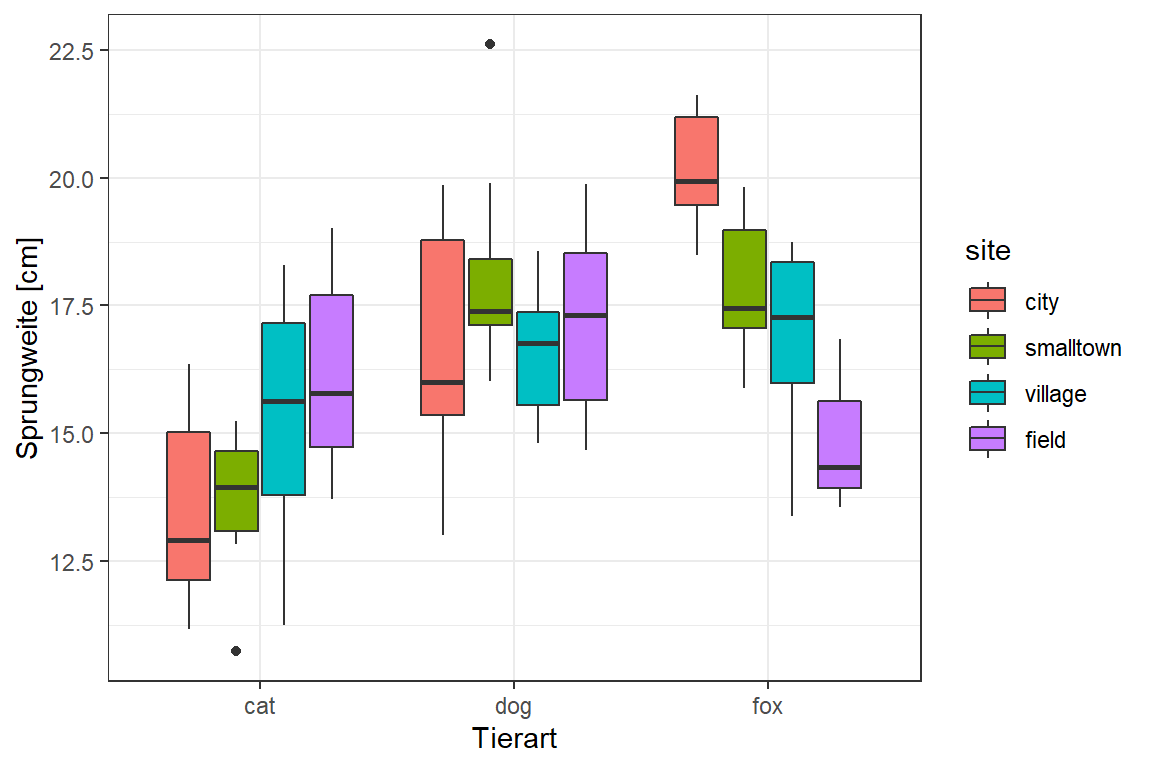
\includegraphics{./example-fleas-dogs-cats-foxes-site_files/figure-pdf/fig-example-4-1.pdf}

}

\caption{\label{fig-example-4}Boxplot der Sprungweiten {[}cm{]} für
Hunde-, Katzen- und Fuchsflöhe in verschiedenen Habitaten.}

\end{figure}

\begin{tcolorbox}[enhanced jigsaw, bottomrule=.15mm, toptitle=1mm, colbacktitle=quarto-callout-tip-color!10!white, opacityback=0, bottomtitle=1mm, leftrule=.75mm, toprule=.15mm, breakable, rightrule=.15mm, title=\textcolor{quarto-callout-tip-color}{\faLightbulb}\hspace{0.5em}{Datei für von Flöhen auf Tieren in Habitaten}, coltitle=black, colframe=quarto-callout-tip-color-frame, colback=white, titlerule=0mm, left=2mm, arc=.35mm, opacitybacktitle=0.6]
Du findest die Datei \texttt{flea\_dog\_cat\_fox\_site.xlsx} auf GitHub
\href{https://github.com/jkruppa/jkruppa.github.io/tree/master/data}{jkruppa.github.io/data/}
als Excel oder auch als CSV.
\end{tcolorbox}

\hypertarget{sec-example-5}{%
\chapter{Von vielen Flöhen auf Hunden und Katzen}\label{sec-example-5}}

Wir schauen uns in diesem Beispiel wiederum nur zwei Tierarten an: Hunde
und Katzen. Auf diesen Tierarten messen wir wieder die Sprunglänge in
{[}cm{]} von jeweils 400 Tieren. Im Vergleich zu dem vorherigen Beispiel
erweitern wir die Daten um eine Spalte \texttt{jump\_weight} in {[}mg{]}
sowie \texttt{sex} {[}male, female{]}. Es ergibt sich folgende
Tabelle~\ref{tbl-example-5} mit den ersten zehn Beobachtungen und die
dazugehörige Abbildung~\ref{fig-example-5}.

\hypertarget{tbl-example-5}{}
\begin{longtable}[]{@{}cccc@{}}
\caption{\label{tbl-example-5}Sprunglängen {[}cm{]}, Gewichte {[}mg{]},
Geschecht {[}sex{]} für Hunde- und Katzenflöhe.}\tabularnewline
\toprule()
animal & sex & weight & jump\_length \\
\midrule()
\endfirsthead
\toprule()
animal & sex & weight & jump\_length \\
\midrule()
\endhead
cat & male & 6.02 & 16.93 \\
cat & male & 5.99 & 16.22 \\
cat & male & 8.05 & 18.96 \\
cat & male & 6.71 & 19.83 \\
cat & male & 6.19 & 17.37 \\
cat & male & 8.18 & 14.45 \\
cat & male & 7.46 & 15.46 \\
cat & male & 5.58 & 15.81 \\
cat & male & 6.19 & 19.14 \\
cat & male & 7.53 & 15.72 \\
\bottomrule()
\end{longtable}

{\marginnote{\begin{footnotesize}Über die explorative Datenanalyse
erfährst du mehr im Kapitel~\ref{sec-eda-ggplot}\end{footnotesize}}}

Die Datentabelle ist in dieser Form schon fast nicht mehr überschaubar.
Daher hilft hier die explorative Datenanalyse weiter. Wir schauen uns
daher die Daten einmal als einen Scatterplot in
Abbildung~\ref{fig-example-5} an. Wir sehen hier, dass wir das mit dem
Gewicht {[}mg{]} der Flöhe auch die Sprungweite in {[}cm{]} steigt.

\begin{figure}

{\centering 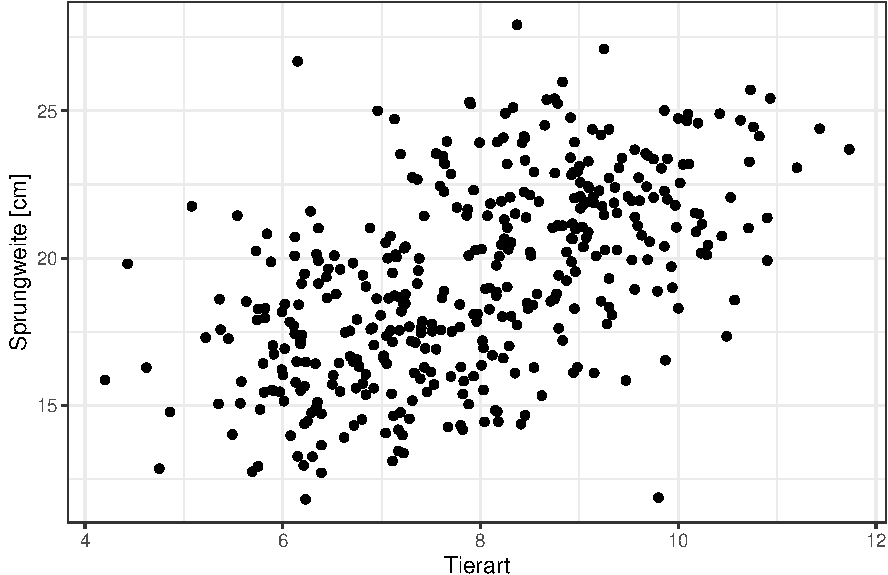
\includegraphics{./example-fleas-dogs-cats-length-weight_files/figure-pdf/fig-example-5-1.pdf}

}

\caption{\label{fig-example-5}Scatterplot der Sprunglängen {[}cm{]} und
Gewichte {[}mg{]} für Hunde- und Katzenflöhe.}

\end{figure}

\begin{tcolorbox}[enhanced jigsaw, bottomrule=.15mm, toptitle=1mm, colbacktitle=quarto-callout-tip-color!10!white, opacityback=0, bottomtitle=1mm, leftrule=.75mm, toprule=.15mm, breakable, rightrule=.15mm, title=\textcolor{quarto-callout-tip-color}{\faLightbulb}\hspace{0.5em}{Datei für von vielen Flöhen auf Hunden und Katzen}, coltitle=black, colframe=quarto-callout-tip-color-frame, colback=white, titlerule=0mm, left=2mm, arc=.35mm, opacitybacktitle=0.6]
Du findest die Datei \texttt{flea\_dog\_cat\_length\_weight.xlsx} auf
GitHub
\href{https://github.com/jkruppa/jkruppa.github.io/tree/master/data}{jkruppa.github.io/data/}
als Excel oder auch als CSV.
\end{tcolorbox}

\part{Programmieren in R}

Was solltest du nun zuerst Lesen? Es ist sehr schwierig die
Programmierung exakt so zu schreiben, dass das Programmieren
\emph{linear} verständlich ist. Du brauchst im Prinzip das Wissen aus
Kapitel~\ref{sec-basics} \emph{Operatoren, Funktionen und Pakete} um die
Grundlagen zu verstehen. Auf der anderen Seite fehlt dir vielleicht noch
das Verständnis von Buchstaben und Zahlen in R. Diesen Zusammenhang
zwischen Buchstaben und Zahlen erkläre ich als erstes im folgenden
Kapitel~\ref{sec-letter-number} \emph{Von Buchstaben und Zahlen}.

Im vorherigen Kapitel zu den Beispielen haben wir die Datentabelle
Tabelle~\ref{tbl-dog-cat-long} mit den Hunde- und Katzenflöhen
erschaffen. Bevor wir uns weiter mit statistischen Kennzahlen
beschäftigen, wollen wir uns einmal die Realisierung der Tabelle
Tabelle~\ref{tbl-dog-cat-long} mit den Hunde- und Katzenflöhen in R
anschauen. Dabei wollen wir auch Eigenschaften von Zahlen und Buchstaben
lernen, die notwendig sind um mit einem Programm wie R kommunizieren zu
können. Wir wollen später R nutzen um die explorative Datenanalyse
anzuwenden. Über die explorative Datenanalyse lernen wir in späteren
Kapiteln mehr.

\begin{tcolorbox}[enhanced jigsaw, bottomrule=.15mm, toptitle=1mm, colbacktitle=quarto-callout-tip-color!10!white, opacityback=0, bottomtitle=1mm, leftrule=.75mm, toprule=.15mm, breakable, rightrule=.15mm, title=\textcolor{quarto-callout-tip-color}{\faLightbulb}\hspace{0.5em}{Einführung in R per Video}, coltitle=black, colframe=quarto-callout-tip-color-frame, colback=white, titlerule=0mm, left=2mm, arc=.35mm, opacitybacktitle=0.6]
Du findest auf YouTube
\href{https://www.youtube.com/playlist?list=PLe51bCp9JvEFUnFqaJG5aRmON9i1ZbOYC}{Grundlagen
in R} als Video Reihe. Ich werde zwar alles nochmal hier als Text
aufschreiben, aber manchmal ist das Sehen und Hören dann einfacher.
\end{tcolorbox}

\hypertarget{sec-letter-number}{%
\chapter{Von Buchstaben und Zahlen}\label{sec-letter-number}}

Im Kapitel~\ref{sec-example-2} haben wir uns folgende Daten in
Tabelle~\ref{tbl-dog-cat-letter} angeschaut. Bevor wir uns weiter mit
statistischen Kennzahlen beschäftigen, wollen wir uns einmal die
Realisierung der Tabelle Tabelle~\ref{tbl-dog-cat-letter} in R
anschauen. Das heist, wie ist eine Tabelle in R aufgebaut und was sehen
wir da eigentlich?

\hypertarget{tbl-dog-cat-letter}{}
\begin{longtable}[]{@{}ccccc@{}}
\caption{\label{tbl-dog-cat-letter}Sprunglängen {[}cm{]} für Hunde- und
Katzenflöhe.}\tabularnewline
\toprule()
animal & jump\_length & flea\_count & grade & infected \\
\midrule()
\endfirsthead
\toprule()
animal & jump\_length & flea\_count & grade & infected \\
\midrule()
\endhead
dog & 5.7 & 18 & 8 & FALSE \\
dog & 8.9 & 22 & 8 & TRUE \\
dog & 11.8 & 17 & 6 & TRUE \\
dog & 8.2 & 12 & 8 & FALSE \\
dog & 5.6 & 23 & 7 & TRUE \\
dog & 9.1 & 18 & 7 & FALSE \\
dog & 7.6 & 21 & 9 & FALSE \\
cat & 3.2 & 12 & 7 & TRUE \\
cat & 2.2 & 13 & 5 & FALSE \\
cat & 5.4 & 11 & 7 & FALSE \\
cat & 4.1 & 12 & 6 & FALSE \\
cat & 4.3 & 16 & 6 & TRUE \\
cat & 7.9 & 9 & 6 & FALSE \\
cat & 6.1 & 7 & 5 & FALSE \\
\bottomrule()
\end{longtable}

Dabei wollen wir auch Eigenschaften von Zahlen und Buchstaben lernen,
die notwendig sind um mit einem Programm wie R kommunizieren zu können.
Nun haben wir Tabelle Tabelle~\ref{tbl-dog-cat-letter} mit Daten zu
verschiedenen Oucomes, wie Sprungweite {[}cm{]}, Anzahl an Flöhen auf
Hunden und Katzen, die Boniturnoten oder aber den Infektionsstatus. Die
Tabelle Tabelle~\ref{tbl-dog-cat-letter} ist zwar nicht groß aber auch
nicht wirklich klein. Wir wollen uns nun damit beschäftigen, die Zahlen
sinnvoll in R darzustellen. Wir wollen mit der Darstellung einer
Datentabelle in R beginnen, einem \texttt{tibble()}.

\hypertarget{daten-in-r-sind-tibble}{%
\section{\texorpdfstring{Daten in R sind
\texttt{tibble()}}{Daten in R sind tibble()}}\label{daten-in-r-sind-tibble}}

Im folgenden sehen wir die Datentabelle Tabelle~\ref{tbl-dog-cat-letter}
in R als \texttt{tibble} dargestellt. Was ist nun ein \texttt{tibble}?
Ein \texttt{tibble} ist zu aller erst ein Speicher für Daten in R. Das
heist wir haben Spalten und Zeilen. Jede Spalte repräsentiert eine
Messung oder Variable und die Zeilen jeweils eine Beobachtung.

\begin{verbatim}
# A tibble: 14 x 5
   animal jump_length flea_count grade infected
   <chr>        <dbl>      <int> <dbl> <lgl>   
 1 dog            5.7         18     8 FALSE   
 2 dog            8.9         22     8 TRUE    
 3 dog           11.8         17     6 TRUE    
 4 dog            8.2         12     8 FALSE   
 5 dog            5.6         23     7 TRUE    
 6 dog            9.1         18     7 FALSE   
 7 dog            7.6         21     9 FALSE   
 8 cat            3.2         12     7 TRUE    
 9 cat            2.2         13     5 FALSE   
10 cat            5.4         11     7 FALSE   
11 cat            4.1         12     6 FALSE   
12 cat            4.3         16     6 TRUE    
13 cat            7.9          9     6 FALSE   
14 cat            6.1          7     5 FALSE   
\end{verbatim}

Als erstes erfahren wir, dass wir einen \texttt{A\ tibble:\ 14\ x\ 5}
vorliegen haben. Das heist, wir haben 14 Zeile und 5 Spalten. In einem
\texttt{tibble} wird immer in der ersten Zeile angezeigt wieviele
Beobachtungen wir in dem Datensatz haben. Wenn das \texttt{tibble} zu
groß wird, werden wir nicht mehr das ganze \texttt{tibble} sehen sondern
nur noch einen Ausschnitt. Im Weiteren hat jede Spalte noch eine
Eigenschaft unter dem Spaltennamen:

\begin{itemize}
\tightlist
\item
  \texttt{\textless{}chr\textgreater{}} bedeutet \texttt{character}. Wir
  haben also hier Worte vorliegen.
\item
  \texttt{\textless{}dbl\textgreater{}} bedeutet \texttt{double}. Ein
  \texttt{double} ist eine Zahl mit Kommastellen.
\item
  \texttt{\textless{}int\textgreater{}} bedeutet \texttt{integer}. Ein
  \texttt{integer} ist eine ganze Zahl ohne Kommastellen.
\item
  \texttt{\textless{}lgl\textgreater{}} bedeutet \texttt{logical} oder
  \texttt{boolean}. Hier gibt es nur die Ausprägung \emph{wahr} oder
  \emph{falsch}. Somit \texttt{TRUE} oder \texttt{FALSE}. Statt den
  Worten \texttt{TRUE} oder \texttt{FALSE} kann hier auch 0 oder 1
  stehen.
\item
  \texttt{\textless{}str\textgreater{}} bedeutet \texttt{string} der aus
  verschiedenen \texttt{character} besteht kann, getrennt durch
  Leerzeichen.
\end{itemize}

\begin{tcolorbox}[enhanced jigsaw, bottomrule=.15mm, toptitle=1mm, colbacktitle=quarto-callout-tip-color!10!white, opacityback=0, bottomtitle=1mm, leftrule=.75mm, toprule=.15mm, breakable, rightrule=.15mm, title=\textcolor{quarto-callout-tip-color}{\faLightbulb}\hspace{0.5em}{Zahlen, Buchstaben, Skalenniveau - Was ist das eigentlich?}, coltitle=black, colframe=quarto-callout-tip-color-frame, colback=white, titlerule=0mm, left=2mm, arc=.35mm, opacitybacktitle=0.6]
Du findest auf YouTube \href{https://youtu.be/OnRaSmybhOQ}{Einführung in
R - Teil 06 - Zahlen, Buchstaben, Skalenniveau - Was ist das
eigentlich?} als Video. Hier erkläre ich den Zusammenhang nochmal in
einem Video.
\end{tcolorbox}

\hypertarget{faktoren-als-wuxf6rter-zu-zahlen}{%
\section{Faktoren als Wörter zu
Zahlen}\label{faktoren-als-wuxf6rter-zu-zahlen}}

{\marginnote{\begin{footnotesize}Ein \textbf{Faktor} ist eine Variable
mit mehrern \textbf{Faktorstufen} oder \textbf{Leveln}. Für uns sieht
der Faktor wie ein Wort aus, hinter jedem Wort steht aber eine Zahl mit
der gerechnet werden kann.\end{footnotesize}}}

Ein Computer und somit auch eine Programmsprache wie R kann keine
Buchstaben \emph{verrechnen}. Ein Programm kann nur mit Zahlen rechnen.
Wir haben aber in der Datentabelle Tabelle~\ref{tbl-dog-cat-letter} in
der Spalte \texttt{animal} Buchstaben stehen. Da wir hier einen
Kompromiss eingehen müssen führen wir Faktoren ein. Ein Faktor
kombiniert Buchstaben mit Zahlen. Wir als Anwender sehen die Buchstaben,
die Wörter bilden. Intern steht aber jedes Wort für eine Zahl, so dass R
mit den Zahlen rechnen kann. Klingt ein wenig kryptisch, aber wir
schauen uns einen \texttt{factor} einmal an.

\begin{Shaded}
\begin{Highlighting}[]
\NormalTok{data\_tbl}\SpecialCharTok{$}\NormalTok{animal[}\DecValTok{1}\SpecialCharTok{:}\DecValTok{8}\NormalTok{]}
\end{Highlighting}
\end{Shaded}

\begin{verbatim}
[1] "dog" "dog" "dog" "dog" "dog" "dog" "dog" "cat"
\end{verbatim}

Was haben wir gemacht? Als erstes haben wir die Spalte \texttt{animal}
aus dem Datensatz \texttt{data\_tbl} mit dem Dollarzeichen \texttt{\$}
\emph{herausgezogen}. Mit dem \texttt{\$} Zeichen können wir uns eine
einzelne Spalte aus dem Datensatz \texttt{data\_tbl} rausziehen. Du
kannst dir das \texttt{\$} wie einen Kleiderbügel und das
\texttt{data\_tbl} als einen Schrank für Kleiderbügel verstellen. An dem
Kleiderbügel hängen dann die einzelnen Zahlen und Worte. Wir nehmen aber
nicht den ganzen Vektor sondern nur die Zahlen 1 bis 8, dargestellt
durch \texttt{{[}1:8{]}}. Die Gänsefüße \texttt{"} um \texttt{dog}
zeigen uns, dass wir hier Wörter oder \texttt{character}vorliegen haben.
Schauen wir auf das Ergebnis, so erhalten wir sieben Mal \texttt{dog}
und einmal \texttt{cat}. Insgesamt die ersten acht Einträge der
Datentabelle. Wir wollen diesen Vektor uns nun einmal als Faktor
anschauen. Wir nutzen die Funktion \texttt{as\_factor()}.
{\marginnote{\begin{footnotesize}Über Funktionen kannst du im
Kapitel~\ref{sec-R-function} mehr erfahren.\end{footnotesize}}}

\begin{Shaded}
\begin{Highlighting}[]
\FunctionTok{as.factor}\NormalTok{(data\_tbl}\SpecialCharTok{$}\NormalTok{animal[}\DecValTok{1}\SpecialCharTok{:}\DecValTok{8}\NormalTok{])}
\end{Highlighting}
\end{Shaded}

\begin{verbatim}
[1] dog dog dog dog dog dog dog cat
Levels: cat dog
\end{verbatim}

Im direkten vergleich verschwinden die Gänsefüße \texttt{"} um
\texttt{dog} und zeigen usn, dass wir hier keine \texttt{character} mehr
vorliegen haben. Darüber hinaus sehen wir auch, dass die der Faktor
jetzt \texttt{Levels} hat. Exakt zwei Stück. Jeweils einen für
\texttt{dog} und einen für \texttt{cat}. Wir werden später Faktoren
benötigen, wenn wir zum Beispiel eine einfaktorielle ANOVA rechnen. Hier
siehst du schon den Begriff \emph{Faktor} wieder.

\marginnote{\begin{footnotesize}

Wir brauchen später zum Modellieren einen Datensatz, der \emph{meist}
aus einer \textbf{Outcome}-Spalte, einer \textbf{Faktor}-Spalte mit der
\emph{Behandlung} und einer \textbf{Faktor}-Spalte mit dem \emph{Block}
oder \emph{Cluster} besteht.

\[
{\small Outcome \sim Behandlung + Block}
\]

\end{footnotesize}}

\hypertarget{von-wuxf6rtern-und-objekten}{%
\section{Von Wörtern und Objekten}\label{von-wuxf6rtern-und-objekten}}

Das mag etwas verwirrend sein, denn es gibt in R Wörter
\texttt{string\ \textless{}str\textgreater{}} oder
\texttt{character\ \textless{}chr\textgreater{}}. Wörter sind was
anderes als Objekte. Streng genommen sind beides Wörter, aber in
Objekten werden Dinge gespeichert wohin gegen das Wort einfach ein Wort
ist. Deshalb kennezeichnen wir Wörter auch mit Gänsefüßchen als win
\texttt{"wort"} und zeigen damit, dass es sich hier um einen String
handelt.

Wir tippen \texttt{"animal"} in R und erhalten \texttt{"animal"} als
Wort zurück. Das sehen wir auch an dem Ausdruck mit den Gänsefüßchen.

\begin{Shaded}
\begin{Highlighting}[]
\StringTok{"animal"}
\end{Highlighting}
\end{Shaded}

\begin{verbatim}
[1] "animal"
\end{verbatim}

{\marginnote{\begin{footnotesize}Über den Zuweisungspfeil
\texttt{\textless{}-} kannst du im Kapitel~\ref{sec-R-pfeil} mehr
erfahren.\end{footnotesize}}}

Wir tippen \texttt{animal} ohne die Anführungszeichen in R und erhalten
den Inhalt von \texttt{animal} ausgegeben. Dafür müssen wir aber das
Objekt \texttt{animal} erst einmal über den Zuweisungspfeil
\texttt{\textless{}-}erschaffen.

\begin{Shaded}
\begin{Highlighting}[]
\NormalTok{animal }\OtherTok{\textless{}{-}} \FunctionTok{c}\NormalTok{(}\StringTok{"dog"}\NormalTok{, }\StringTok{"cat"}\NormalTok{, }\StringTok{"fox"}\NormalTok{)}
\NormalTok{animal}
\end{Highlighting}
\end{Shaded}

\begin{verbatim}
[1] "dog" "cat" "fox"
\end{verbatim}

Sollte es das Objekt \texttt{animal} nicht geben, also nicht über den
Zuweisungspfeil \texttt{\textless{}-} erschaffen worden, dann wird eine
Fehlermeldung von R ausgegeben:

\texttt{Fehler\ in\ eval(expr,\ envir,\ enclos)\ :\ Objekt\ \textquotesingle{}animal\textquotesingle{}\ nicht\ gefunden}

\hypertarget{zusammenfassung}{%
\section{Zusammenfassung}\label{zusammenfassung}}

{\marginnote{\begin{footnotesize}\textbf{Variablennamen} meint hier
immer den \textbf{Namen der Spalte} im Datensatz bzw.
\texttt{tibble}\end{footnotesize}}}

Tabelle~\ref{tbl-skalenniveau} zeigt eine Übersicht wie einzelne
Variablennamen und deren zugehörigen Beispielen sowie den Namen in R,
der Informatik allgemein, als Skalenneivau und welcher
Verteilungsfamilie die Variable angehören würde. Leider ist es so, dass
wieder gleiche Dinge unterschiedliche benannt werden. Aber an dieses
doppelte Benennen können wir uns in der Statistik schonmal gewöhnen.

\begin{figure*}

\hypertarget{tbl-skalenniveau}{}
\begin{longtable}[]{@{}
  >{\raggedright\arraybackslash}p{(\columnwidth - 10\tabcolsep) * \real{0.1181}}
  >{\raggedright\arraybackslash}p{(\columnwidth - 10\tabcolsep) * \real{0.2283}}
  >{\raggedright\arraybackslash}p{(\columnwidth - 10\tabcolsep) * \real{0.0866}}
  >{\raggedright\arraybackslash}p{(\columnwidth - 10\tabcolsep) * \real{0.1417}}
  >{\raggedright\arraybackslash}p{(\columnwidth - 10\tabcolsep) * \real{0.2677}}
  >{\raggedright\arraybackslash}p{(\columnwidth - 10\tabcolsep) * \real{0.1575}}@{}}
\caption{\label{tbl-skalenniveau}Zusammenfassung und Übersicht von
Variablennamen und deren Bennung in R, in der Informatik allgemein, als
Skalenniveau und die dazugehörige Verteilungsfamilie.}\tabularnewline
\toprule()
\begin{minipage}[b]{\linewidth}\raggedright
Variablenname
\end{minipage} & \begin{minipage}[b]{\linewidth}\raggedright
Beispiel
\end{minipage} & \begin{minipage}[b]{\linewidth}\raggedright
R
\end{minipage} & \begin{minipage}[b]{\linewidth}\raggedright
Infomatik
\end{minipage} & \begin{minipage}[b]{\linewidth}\raggedright
Skalenniveau
\end{minipage} & \begin{minipage}[b]{\linewidth}\raggedright
Verteilungsfamilie
\end{minipage} \\
\midrule()
\endfirsthead
\toprule()
\begin{minipage}[b]{\linewidth}\raggedright
Variablenname
\end{minipage} & \begin{minipage}[b]{\linewidth}\raggedright
Beispiel
\end{minipage} & \begin{minipage}[b]{\linewidth}\raggedright
R
\end{minipage} & \begin{minipage}[b]{\linewidth}\raggedright
Infomatik
\end{minipage} & \begin{minipage}[b]{\linewidth}\raggedright
Skalenniveau
\end{minipage} & \begin{minipage}[b]{\linewidth}\raggedright
Verteilungsfamilie
\end{minipage} \\
\midrule()
\endhead
weight & 12.3, 12.4, 5.4, 21.3, 13.4 & numeric & double & continuous &
Gaussian \\
count & 5, 0, 12, 23, 1, 4, 21 & integer & integer & continuous &
Poisson \\
dosis & low, mid, high & ordered & & categorical / discrete / ordinal &
Ordinal \\
field & mainz, berlin, kiel & factor & & categorical / discrete &
Multinomial \\
cancer & 0, 1 & factor & & dichotomous / binary / nominal & Binomial \\
treatment & ``placebo'', ``aspirin'' & character & character/string &
dichotomous / binary / nominal & Binomial \\
birth & 2001-12-02, 2005-05-23 & date & & & \\
\bottomrule()
\end{longtable}

\end{figure*}

\hypertarget{sec-basics}{%
\chapter{Operatoren, Funktionen und Pakete}\label{sec-basics}}

Es ist immer schwierig, wann die Grundlagen von R einmal gelehrt werden
sollte. Wenn du nichts von Programmierung bis jetzt gehört hast, dann
mag es keinen Sinn ergeben mit Operatoren, wie dem Zuweisungspfeil
\texttt{\textless{}-} und der Pipe \texttt{\%\textgreater{}\%} zu
beginnen. Wir brauchen aber für die Programmierung folgende zentrale
Konzepte.

\begin{itemize}
\tightlist
\item
  Wir müssen zusätzliche Pakete in R installieren und laden können
  (siehe Kapitel~\ref{sec-R-packages}).
\item
  Wir müssen verstehen wie wir uns einen Vektor mit \texttt{c()} bauen
  (siehe Kapitel~\ref{sec-R-vector}).
\item
  Wir müssen wissen was eine Funktion in R ist (siehe
  Kapitel~\ref{sec-R-function}).
\item
  Wir müssen den Operator Zuweisungspfeil \texttt{\textless{}-}
  verstehen und anwenden können (siehe Kapitel~\ref{sec-R-pfeil}).
\item
  Wir müssen den Operator Pipe \texttt{\%\textgreater{}\%} verstehen und
  anwenden können (siehe Kapitel~\ref{sec-R-pipe}).
\item
  Wir müssen den Operator \texttt{\$} verstehen, da manche Funktionen in
  R nicht mit Datensätzen sondenr nur mit Vektoren arbeiten können
  (siehe Kapitel~\ref{sec-dollar}).
\item
  Wir müssen verstehen wie wir ein Modell in R mit der Tilde
  \texttt{\textasciitilde{}} definieren (siehe
  Kapitel~\ref{sec-formula}).
\item
  Wir müssen wissen und verstehen wie wir mit \texttt{?} englische
  Hilfeseiten öffnen können (siehe Kapitel~\ref{sec-R-help}).
\end{itemize}

Nicht alle Konzepte brauchst du \emph{unmittelbar} aber ich nutze diese
Konzepte wiederholt in allen Kapiteln, so dass du hier immer wieder mal
schauen kannst, was die Grundlagen sind.

\hypertarget{sec-R-packages}{%
\section{\texorpdfstring{Pakete und
\texttt{library()}}{Pakete und library()}}\label{sec-R-packages}}

{\marginnote{\begin{footnotesize}Als Vanilla beschreibt man in der
Informatikerwelt ein Programm, was keine zusätzlichen Pakete geladen
hat. Also die reinst Form ohne zusätzlichen
Geschmack.\end{footnotesize}}}

In der \emph{Vanilla}-Variante hat R sehr wenige Funktionen. Ohne
zusätzliche Pakete ist R mehr ein sehr potenter Taschenrechner. Leider
mit der Funktionalität aus den 90'zigern, was die Programmierumgebung
und die Funktionen angeht. Das wollen wir aber nicht. Wir wollen auf den
aktuellen Stand der Technik und auch Sprache programmieren. Daher nutzen
wir zusätzliche R Pakete.

\begin{figure}

{\centering 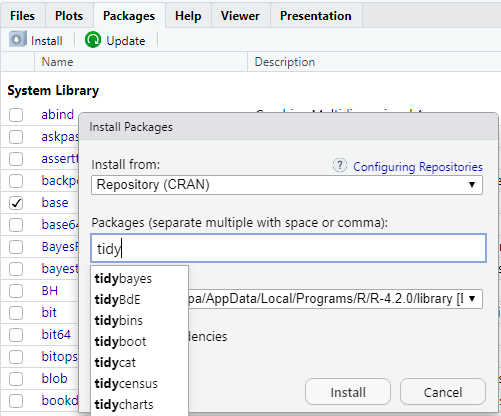
\includegraphics[width=0.8\textwidth,height=\textheight]{./images/programing_01.PNG}

}

\caption{\label{fig-pro-01}Auf den Reiter \emph{Packages} klicken und
dann \emph{Install}. In der deutschen version vom RStudio mögen die
Begriffe leicht anders sein.}

\end{figure}

In Abbildung~\ref{fig-pro-01} wird gezeigt wie du ein zusätzliches Paket
installieren kannst. Hierbei ist nochmal wichtig den semantischen
Unterschied zu wissen. Es gibt das Paket \texttt{tidyverse} was wir viel
nutzen. Wir isnatllieren \emph{einmalig} Pakete der Funktion
\texttt{install.packages()} oder eben wie in Abbildung~\ref{fig-pro-01}
gezeigt. Wir nutzen die Funktion \texttt{library()} um ein Paket in R zu
laden. Ja, es müsste anders heisen, tut es aber nicht.

\begin{Shaded}
\begin{Highlighting}[]
\DocumentationTok{\#\# Das Paket tidyverse installieren {-} einmalig}
\FunctionTok{install.packages}\NormalTok{(tidyverse)}

\DocumentationTok{\#\# Das Paket tidyverse laden {-} jedes Mal}
\FunctionTok{library}\NormalTok{(tidyverse)}
\end{Highlighting}
\end{Shaded}

Nun muss man sich immer merken, ob das Paket schon installiert ist oder
man schreibt relativ viele \texttt{library()} untereinander. Das
passiert schnell, wenn du viele Pakete laden willst. Dafür erlaubt dir
das Paket \texttt{pacman} eine Vereinfachung. Die Funktion
\texttt{p\_load()} installiert Pakete, wenn die Pakete nicht installiert
sind. Sollten die Pakete installiert sein, so werden die Pakete geladen.
Du musst nur einmal \texttt{install.packages(pacman)} ausführen um das
Paket \texttt{pacman} zu installieren.

\begin{Shaded}
\begin{Highlighting}[]
\NormalTok{pacman}\SpecialCharTok{::}\FunctionTok{p\_load}\NormalTok{(tidyverse, magrittr, readxl)}
\end{Highlighting}
\end{Shaded}

Schlussendlich gibt es noch die Möglichkeit sich alles nochmal bei
YouTube anzuschauen.

\begin{tcolorbox}[enhanced jigsaw, bottomrule=.15mm, toptitle=1mm, colbacktitle=quarto-callout-tip-color!10!white, opacityback=0, bottomtitle=1mm, leftrule=.75mm, toprule=.15mm, breakable, rightrule=.15mm, title=\textcolor{quarto-callout-tip-color}{\faLightbulb}\hspace{0.5em}{Unterschied von Packages und Libraries in R}, coltitle=black, colframe=quarto-callout-tip-color-frame, colback=white, titlerule=0mm, left=2mm, arc=.35mm, opacitybacktitle=0.6]
Du findest auf YouTube \href{https://youtu.be/TWimhd3ZyMM}{Einführung in
R - Teil 03 - Unterschied Packages und Libraries in R} als Video. Hier
erkläre ich nochmal den Ablauf zwischen Installieren eines Paketes und
dem Laden eines Paketes.
\end{tcolorbox}

\hypertarget{sec-R-vector}{%
\section{\texorpdfstring{Einen Vektor bauen
\texttt{c()}}{Einen Vektor bauen c()}}\label{sec-R-vector}}

Wir können mit der Funktion \texttt{c()} Zahlen und Wörter zu einem
Vektor kombinieren.

\begin{Shaded}
\begin{Highlighting}[]
\FunctionTok{c}\NormalTok{(}\StringTok{"dog"}\NormalTok{, }\StringTok{"dog"}\NormalTok{, }\StringTok{"cat"}\NormalTok{, }\StringTok{"cat"}\NormalTok{, }\StringTok{"fox"}\NormalTok{, }\StringTok{"fox"}\NormalTok{)}
\end{Highlighting}
\end{Shaded}

\begin{verbatim}
[1] "dog" "dog" "cat" "cat" "fox" "fox"
\end{verbatim}

Hier werden die Wörter ``dog'', ``cat'' und ``fox'' miteinader in einen
Vektor kombiniert. Wir erinnern uns an das \texttt{\$} Zeichen, was uns
erlaubt eine Variable als Vektor aus einem
\texttt{tibble()}herauszuziehen.

\hypertarget{sec-R-function}{%
\section{Funktionen}\label{sec-R-function}}

Wir haben schon einige Funktion nebenbei in R kennengelernt. Zum einen
\texttt{as.factor()} um einen Faktor zu erstellen oder aus dem
Kapitel~\ref{sec-R-packages}, wo wir die Funktion
\texttt{install.packages()} nutzen um ein Paket zu installieren oder
aber die Funktion \texttt{library()} um ein Paket in R zu laden.

Funktionen sehen aus wie Wörter. Haben aber keine Gänsefüßchen und
beinhalten auch keine Daten oder Vektoren. Funktionen können mit Daten
und Vektoren rechnen und geben das Berechnete dann wieder. Nehmen wir
als Beispiel die Funktion \texttt{mean()}, die den Mittelwert von einer
Reihe Zahlen berechnet.

\begin{Shaded}
\begin{Highlighting}[]
\NormalTok{y }\OtherTok{\textless{}{-}} \FunctionTok{c}\NormalTok{(}\FloatTok{1.2}\NormalTok{, }\FloatTok{3.4}\NormalTok{, }\FloatTok{2.1}\NormalTok{, }\DecValTok{6}\NormalTok{, }\FloatTok{4.3}\NormalTok{)}
\FunctionTok{mean}\NormalTok{(y)}
\end{Highlighting}
\end{Shaded}

\begin{verbatim}
[1] 3.4
\end{verbatim}

Wir sehen, dass wir mit der Funktion \texttt{c()} die Zahlen
\(1.2, 3.4, 2.1, 6, 4.3\) zusammenkleben. Danach speichern wir die
Zahlen in den Objekt \texttt{y} als einen Vektor ab. Wir müssen
\texttt{y}nicht erst erschaffen, das Erschaffen und Speichern passiert
in R in einem Schritt. Wir stecken nun den Vektor \texttt{y} in die
Funktion \texttt{mean()} und erhalten den Mittelwert von \(3.4\) der
Zahlen wiedergegeben.

{\marginnote{\begin{footnotesize}Eigentlich müssen in der Programmierung
Objekte erst \textbf{deklariert} werden und somit erschaffen. Erst dann
können Objekte \textbf{initalisiert} und somit befüllt bzw. etwas
zugewiesen werden.\end{footnotesize}}}

\hypertarget{sec-R-pfeil}{%
\section{\texorpdfstring{Zuweisungspfeil
\texttt{\textless{}-}}{Zuweisungspfeil \textless-}}\label{sec-R-pfeil}}

Mit dem Zuweisungspfeil speichern wir \emph{Dinge} in Objekte in R. Das
heist wir speichern damit intern in R Datensätze und viele andere
Sachen, die wir dan später wieder verwenden wollen. Schauen wir uns das
einmal im Beispiel an. Schrieben wir nur den Vektor \texttt{c()} mit
Hunden und Katzen darin, so erscheint eine Ausgabe in R.

\begin{Shaded}
\begin{Highlighting}[]
\FunctionTok{c}\NormalTok{(}\StringTok{"dog"}\NormalTok{, }\StringTok{"dog"}\NormalTok{, }\StringTok{"cat"}\NormalTok{, }\StringTok{"cat"}\NormalTok{, }\StringTok{"fox"}\NormalTok{, }\StringTok{"fox"}\NormalTok{)}
\end{Highlighting}
\end{Shaded}

\begin{verbatim}
[1] "dog" "dog" "cat" "cat" "fox" "fox"
\end{verbatim}

Schreiben wir den gleichen Vektor und nutzen den Zuweisungspfeil, dann
wird der Vektor in dem Objekt \texttt{animal} gespeichert.

\begin{Shaded}
\begin{Highlighting}[]
\NormalTok{animal }\OtherTok{\textless{}{-}} \FunctionTok{c}\NormalTok{(}\StringTok{"dog"}\NormalTok{, }\StringTok{"dog"}\NormalTok{, }\StringTok{"cat"}\NormalTok{, }\StringTok{"cat"}\NormalTok{, }\StringTok{"fox"}\NormalTok{, }\StringTok{"fox"}\NormalTok{)}
\end{Highlighting}
\end{Shaded}

Wie kommen wir jetzt an die Sachen, die in \texttt{animal} drin sind?
Wir können einfach \texttt{animal} in R schreiben und dann wird uns der
Inhalt von \texttt{animal} ausgegeben.

\begin{Shaded}
\begin{Highlighting}[]
\NormalTok{animal}
\end{Highlighting}
\end{Shaded}

\begin{verbatim}
[1] "dog" "dog" "cat" "cat" "fox" "fox"
\end{verbatim}

{\marginnote{\begin{footnotesize}Der Zuweisungspfeil
\texttt{\textless{}-} ist zentral für die Nutzung von
R.\end{footnotesize}}}

Wir nutzen den Zuweisungspfeil \texttt{\textless{}-} ist zentral für die
Nutzung von R. Wir brauchen den Zuweisungspfeil \texttt{\textless{}-} um
Objekte in R zu erschaffen und Ergebnisse intern abzuspeichern. Zusammen
mit Funktionen nutzen wir nur noch die Pipe \texttt{\%\textgreater{}\%}
öfter.

\hypertarget{sec-R-pipe}{%
\section{\texorpdfstring{Pipe
\texttt{\%\textgreater{}\%}}{Pipe \%\textgreater\%}}\label{sec-R-pipe}}

\begin{tcolorbox}[enhanced jigsaw, bottomrule=.15mm, toptitle=1mm, colbacktitle=quarto-callout-tip-color!10!white, opacityback=0, bottomtitle=1mm, leftrule=.75mm, toprule=.15mm, breakable, rightrule=.15mm, title=\textcolor{quarto-callout-tip-color}{\faLightbulb}\hspace{0.5em}{Pipes in R}, coltitle=black, colframe=quarto-callout-tip-color-frame, colback=white, titlerule=0mm, left=2mm, arc=.35mm, opacitybacktitle=0.6]
Du findest auf YouTube \href{https://youtu.be/6u4RR26eqNw}{Einführung in
R - Teil 11 - Pipes in R} als Video. Hier erkläre ich den Zusammenhang
nochmal in einem Video.
\end{tcolorbox}

Im Weiteren nutzen wir den Pipe Operator dargestellt als
\texttt{\%\textbackslash{}\textgreater{}\%}. Du kannst dir den Pipe
Operator als eine Art Röhre vorstellen in dem die Daten verändert werden
und dann an die nächste Funktion weitergeleitet werden. Im folgenden
siehst du viele Funktionen, die aneinander über Objekte miteinander
verbunden werden. Im Kapitel~\ref{sec-dplyr} erfährst du mehr über die
Funktionen \texttt{select()}und \texttt{filter()}.

\begin{Shaded}
\begin{Highlighting}[]
\NormalTok{data\_tbl }\OtherTok{\textless{}{-}} \FunctionTok{read\_excel}\NormalTok{(}\StringTok{"data/flea\_dog\_cat.xlsx"}\NormalTok{)}
\NormalTok{animal\_1\_tbl }\OtherTok{\textless{}{-}} \FunctionTok{select}\NormalTok{(data\_tbl, animal, jump\_length)}
\NormalTok{animal\_2\_tbl }\OtherTok{\textless{}{-}} \FunctionTok{filter}\NormalTok{(animal\_1\_tbl, jump\_length }\SpecialCharTok{\textgreater{}=} \DecValTok{4}\NormalTok{)}
\FunctionTok{sort}\NormalTok{(animal\_2\_tbl}\SpecialCharTok{$}\NormalTok{jump\_length)}
\end{Highlighting}
\end{Shaded}

\begin{verbatim}
 [1]  4.1  4.3  5.4  5.6  5.7  6.1  7.6  7.9  8.2  8.9  9.1 11.8
\end{verbatim}

\begin{Shaded}
\begin{Highlighting}[]
\NormalTok{data\_tbl }\SpecialCharTok{\%\textgreater{}\%} 
  \FunctionTok{select}\NormalTok{(animal, jump\_length) }\SpecialCharTok{\%\textgreater{}\%} 
  \FunctionTok{filter}\NormalTok{(jump\_length }\SpecialCharTok{\textgreater{}=} \DecValTok{4}\NormalTok{) }\SpecialCharTok{\%\textgreater{}\%} 
  \FunctionTok{pull}\NormalTok{(jump\_length) }\SpecialCharTok{\%\textgreater{}\%} 
\NormalTok{  sort}
\end{Highlighting}
\end{Shaded}

\begin{verbatim}
 [1]  4.1  4.3  5.4  5.6  5.7  6.1  7.6  7.9  8.2  8.9  9.1 11.8
\end{verbatim}

Im unteren Beispiel siehst du die Nutzung des Pipe Operators
\texttt{\%\textgreater{}\%}. Das Ergebnis ist das gleiche, aber der Code
ist einfacher zu lesen. Wir nehmen den Datensatz \texttt{data\_tbl}
leiten den Datensatz in den Funktion \texttt{select()} und wählen die
Spalten \texttt{animal} sowie \texttt{jump\_length}. Dann filtern wir
noch nach \texttt{jump\_length}größer als 4 cm. Dann ziehen wir uns mit
der Funktion \texttt{pull()} die Spalte \texttt{jump\_length} aus dem
Datensatz. Den Vektor leiten wir dann weiter in die Funktion
\texttt{sort()} und erhalten die sortierten Sprunglängen zurück.

\hypertarget{sec-dollar}{%
\section{\texorpdfstring{Spalte extrahieren
\texttt{\$}}{Spalte extrahieren \$}}\label{sec-dollar}}

Wir nutzen eigentlich die Funktion \texttt{pull()} um eine Spalte bzw.
Vektor aus einem Datensatz zu extrahieren.

\begin{Shaded}
\begin{Highlighting}[]
\NormalTok{data\_tbl }\SpecialCharTok{\%\textgreater{}\%} 
  \FunctionTok{pull}\NormalTok{(animal)}
\end{Highlighting}
\end{Shaded}

\begin{verbatim}
 [1] "dog" "dog" "dog" "dog" "dog" "dog" "dog" "cat" "cat" "cat" "cat" "cat"
[13] "cat" "cat"
\end{verbatim}

Manche Funktionen in R, besonders die älteren Funktionen, benötigen
keinen Datensatz sondern meist zwei bis drei Vektoren. Das heißt, wir
können nicht einfach einen Datensatz in eine Funktion über
\texttt{data\ =\ data\_tbl} stecken sondern müssen der Funktion Vektoren
übergeben. Dafür nutzen wir den \texttt{\$} Operator.

\begin{Shaded}
\begin{Highlighting}[]
\NormalTok{data\_tbl}\SpecialCharTok{$}\NormalTok{animal}
\end{Highlighting}
\end{Shaded}

\begin{verbatim}
 [1] "dog" "dog" "dog" "dog" "dog" "dog" "dog" "cat" "cat" "cat" "cat" "cat"
[13] "cat" "cat"
\end{verbatim}

\begin{Shaded}
\begin{Highlighting}[]
\NormalTok{data\_tbl}\SpecialCharTok{$}\NormalTok{jump\_length}
\end{Highlighting}
\end{Shaded}

\begin{verbatim}
 [1]  5.7  8.9 11.8  8.2  5.6  9.1  7.6  3.2  2.2  5.4  4.1  4.3  7.9  6.1
\end{verbatim}

Wir werden versuchen diese Schreibweise zu vermeiden, aber manchmal ist
es sehr nützlich die Möglichkeit zu haben auf diese Weise eine Spalte zu
extrahieren.

\hypertarget{sec-formula}{%
\section{\texorpdfstring{Modelle definieren mit
\texttt{formula}}{Modelle definieren mit formula}}\label{sec-formula}}

Wir müssen später Modelle in R definieren um zum Beispiel den t Test
oder aber eine lineare Regression rechnen zu können. Wir nutzen dazu in
R die \texttt{formula} Syntax. Das heißt links von der Tilde
\texttt{\textasciitilde{}} steht das \(y\), also der Spaltenname aus dem
Datensatz \texttt{data\ =} den wir nutzen, der das Outcome
repräsentiert. Rechts von der Tilde \texttt{\textasciitilde{}} stehen
alle \(x_1, ..., x_p\), also alle Spalten aus dem Datensatz
\texttt{data\ =} den wir nutzen, der die Einflussfaktoren repräsentiert.

In unserem Beispiel mit den Hunde- und Katzenflöhen aus
Kapitel~\ref{sec-example-2} wäre das \(y\) die Spalte
\texttt{jump\_length} und das \(x\) der Faktor \texttt{animal}. Wir
erstellen mit der Funktion \texttt{formula()} das Modell in R. Wir
brauchen später die Funktion \texttt{formula} nur implizit, aber hier
ist es gut, das du einmal siehst, wie so eine Formula in R aussieht.

\begin{Shaded}
\begin{Highlighting}[]
\FunctionTok{formula}\NormalTok{(jump\_length }\SpecialCharTok{\textasciitilde{}}\NormalTok{ animal)}
\end{Highlighting}
\end{Shaded}

\begin{verbatim}
jump_length ~ animal
\end{verbatim}

Wenn die Formel sehr lang wird bzw. wir die Namen der Spalten aus
anderen Funktionen haben, können wir auch die Funktion
\texttt{reformulate()} nutzen. Wir brauchen die Funktion aber eher im
Bereich des maschinellen Lernens. Hier ist die Funktion
\texttt{reformulate()} aufgeführt, da es inhaltlich passt.

\begin{Shaded}
\begin{Highlighting}[]
\FunctionTok{reformulate}\NormalTok{(}\AttributeTok{termlabels =} \FunctionTok{c}\NormalTok{(}\StringTok{"animal"}\NormalTok{, }\StringTok{"sex"}\NormalTok{, }\StringTok{"site"}\NormalTok{),}
            \AttributeTok{response =} \StringTok{"jump\_length"}\NormalTok{,}
            \AttributeTok{intercept =} \ConstantTok{TRUE}\NormalTok{)}
\end{Highlighting}
\end{Shaded}

\begin{verbatim}
jump_length ~ animal + sex + site
\end{verbatim}

\hypertarget{sec-R-help}{%
\section{\texorpdfstring{Hilfe mit
\texttt{?}}{Hilfe mit ?}}\label{sec-R-help}}

Das Fragezeichen \texttt{?} vor einem Funktionsnamen erlaubt die
Hilfeseite zu öffnen. Die Hilfsseiten findest du auch in einem der
Reiter im RStudio.

\begin{figure}

{\centering 
\includegraphics{./images/basics-help.png}

}

\caption{\label{fig-basic-01}Neben den Paketen in R findet sich auch der
Reiter Help, wo du Hilfe für die einzelnen Funktionen findets..}

\end{figure}

\hypertarget{daten-einlesen}{%
\chapter{Daten einlesen}\label{daten-einlesen}}

\marginnote{\begin{footnotesize}

Im Anhang~\ref{sec-beispiel-auswertung} findest du Beispiele für die
Auswertung von Daten. Du kannst dir dort das Format anschauen und dann
entsprechend deine Daten formatieren. Du findest auch alle Dateien auf
GitHub unter
\href{https://github.com/jkruppa/jkruppa.github.io/tree/master/data}{jkruppa.github.io/data/}
als Excel oder auch als CSV. Schau dir die Beispiele einmal an.

\end{footnotesize}}

Die Daten aus unserem Experiment müssen rein in R. Das heißt, wir haben
meist unsere Daten in einer Exceldatei vorliegen und wollen diese Daten
nun in R einlesen.

Gängige Fehler beim Einlesen von Dateien in R sind folgende Probelem.
Wir wollen diese Probeleme nacheinander einmal durchgehen. Aber keine
Sorge, das Einlesen von Daten in R ist immer am Anfang etwas frickelig.
Du kannst gerne in das R Tutorium (siehe Kapitel~\ref{sec-r-tutorium}
für Raum und Zeiten) kommen, dann können wir dir da beim Einlesen der
Daten helfen.

\begin{itemize}
\tightlist
\item
  das Format der Daten ist nicht richtig (Kapitel~\ref{sec-format})
\item
  der Pfad zur Datei ist falsch (Kapitel~\ref{sec-pfad})
\item
  in der Datei sind komische Zeichen, wie Umlaute und
  Co.~(Kapitel~\ref{sec-umlaute})
\item
  in der Datei sind Leerzeichen in den Spaltennamen
  (Kapitel~\ref{sec-spalten})
\end{itemize}

\hypertarget{genutzte-r-pakete-fuxfcr-das-kapitel}{%
\section{Genutzte R Pakete für das
Kapitel}\label{genutzte-r-pakete-fuxfcr-das-kapitel}}

Wir wollen folgende R Pakete in diesem Kapitel nutzen.

\begin{Shaded}
\begin{Highlighting}[]
\NormalTok{pacman}\SpecialCharTok{::}\FunctionTok{p\_load}\NormalTok{(tidyverse, magrittr, janitor)}
\end{Highlighting}
\end{Shaded}

Am Ende des Kapitels findest du nochmal den gesamten R Code in einem
Rutsch zum selber durchführen oder aber kopieren.

\hypertarget{sec-format}{%
\section{Dateiformat}\label{sec-format}}

\marginnote{\begin{footnotesize}

Das Buch \emph{Cookbook for R} stellt auch Beispiele für die Funktion
\texttt{gather()} zu Verfügung für die Umwandlung von Wide zu Long
Format:
\href{http://www.cookbook-r.com/Manipulating_data/Converting_data_between_wide_and_long_format/}{Converting
data between wide and long format}

\end{footnotesize}}

Wir unterschieden bei Datenformaten zwischen den Wide Format und dem
Long Format. Meistens gibst du die Daten intuitv im Wide Format in Excel
ein. Das ist in Excel auch übersichtlicher. R und später die Funktion
\texttt{ggplot()} zur Visualisierung der Daten kann aber nur mit dem
Long Format arbeiten. Wir können aber mit der Funktion \texttt{gather()}
das Wide Format in das Long Format umwandeln.

\hypertarget{wide-format}{%
\subsection{Wide Format}\label{wide-format}}

In Tabelle~\ref{tbl-imp-cat-dog-wide} sehen wir eine typische
Datentabelle in einem Wide Format. Die Spalten egeben jeweils die
Tierart wieder und die Einträge in den Spalten sind die Sprungweiten in
{[}cm{]}.

\hypertarget{tbl-imp-cat-dog-wide}{}
\begin{longtable}[]{@{}cc@{}}
\caption{\label{tbl-imp-cat-dog-wide}Eine Datentabelle mit Sprungweiten
in {[}cm{]} von Hunde- und Katzenflöhen im Wide Format.}\tabularnewline
\toprule()
dog & cat \\
\midrule()
\endfirsthead
\toprule()
dog & cat \\
\midrule()
\endhead
5.2 & 10.1 \\
4.9 & 9.4 \\
12.1 & 11.8 \\
8.2 & 6.7 \\
5.6 & 8.2 \\
9.1 & 9.1 \\
7.4 & 7.1 \\
\bottomrule()
\end{longtable}

Wir können diese Datentablle auch in R erstellen und uns als
\texttt{tibble()} wiedergeben lassen.

\begin{Shaded}
\begin{Highlighting}[]
\NormalTok{jump\_wide\_tbl }\OtherTok{\textless{}{-}} \FunctionTok{tibble}\NormalTok{(}\AttributeTok{dog =} \FunctionTok{c}\NormalTok{(}\FloatTok{5.2}\NormalTok{, }\FloatTok{4.9}\NormalTok{, }\FloatTok{12.1}\NormalTok{, }\FloatTok{8.2}\NormalTok{, }\FloatTok{5.6}\NormalTok{, }\FloatTok{9.1}\NormalTok{, }\FloatTok{7.4}\NormalTok{),}
                        \AttributeTok{cat =} \FunctionTok{c}\NormalTok{(}\FloatTok{10.1}\NormalTok{, }\FloatTok{9.4}\NormalTok{, }\FloatTok{11.8}\NormalTok{, }\FloatTok{6.7}\NormalTok{, }\FloatTok{8.2}\NormalTok{, }\FloatTok{9.1}\NormalTok{, }\FloatTok{7.1}\NormalTok{))}
\NormalTok{jump\_wide\_tbl}
\end{Highlighting}
\end{Shaded}

\begin{verbatim}
# A tibble: 7 x 2
    dog   cat
  <dbl> <dbl>
1   5.2  10.1
2   4.9   9.4
3  12.1  11.8
4   8.2   6.7
5   5.6   8.2
6   9.1   9.1
7   7.4   7.1
\end{verbatim}

{\marginnote{\begin{footnotesize}Wenn du schon Daten hast, dann macht es
eventuell mehr Sinn eine \textbf{neue} Exceldatei anzulegen in der du
dann die Daten in das Long Format kopierst.\end{footnotesize}}}

Wir können aber mit einem Wide-Format nicht mit \texttt{ggplot()} die
Daten aus der Tabelle~\ref{tbl-imp-cat-dog-wide} visualisieren. Deshalb
müssen wir entweder das Wide Format in das Long Format umwandeln oder
die Daten gleich in Excel im Long Format erstellen.

\hypertarget{long-format}{%
\subsection{Long Format}\label{long-format}}

Wenn du Daten erstellst ist es wichtig, dass du die Daten in Excel im
Long-Format erstellst. Dabei muss eine Beobachtung eine Zeile sein. Du
siehst in Abbildung~\ref{fig-imp-long} ein Beispiel für eine Tabelle in
Excel, die dem Long Format folgt.

\begin{figure}

{\centering 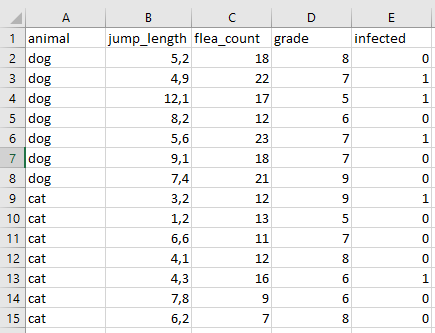
\includegraphics{./images/import_03.PNG}

}

\caption{\label{fig-imp-long}Beispiel für eine Exceldatentabelle in Long
Format.}

\end{figure}

Im Folgenden sehen wir einmal wie die Funktion \texttt{gather()} das
\texttt{tibble()} in Wide Format in ein \texttt{tibble()} in Long Format
umwandelt. Wir müssen dafür noch die Spalte benennen mit der Option
\texttt{key\ =} in die die Namen der Spalten aus dem Wide Format
geschrieben werden sowie den Spaltennamen für die eigentlichen Messwerte
mit der Option \texttt{value\ =}.

\begin{Shaded}
\begin{Highlighting}[]
\NormalTok{jump\_tbl }\OtherTok{\textless{}{-}} \FunctionTok{tibble}\NormalTok{(}\AttributeTok{dog =} \FunctionTok{c}\NormalTok{(}\FloatTok{5.2}\NormalTok{, }\FloatTok{4.9}\NormalTok{, }\FloatTok{12.1}\NormalTok{, }\FloatTok{8.2}\NormalTok{, }\FloatTok{5.6}\NormalTok{, }\FloatTok{9.1}\NormalTok{, }\FloatTok{7.4}\NormalTok{),}
                   \AttributeTok{cat =} \FunctionTok{c}\NormalTok{(}\FloatTok{10.1}\NormalTok{, }\FloatTok{9.4}\NormalTok{, }\FloatTok{11.8}\NormalTok{, }\FloatTok{6.7}\NormalTok{, }\FloatTok{8.2}\NormalTok{, }\FloatTok{9.1}\NormalTok{, }\FloatTok{7.1}\NormalTok{)) }\SpecialCharTok{\%\textgreater{}\%}
  \FunctionTok{gather}\NormalTok{(}\AttributeTok{key =} \StringTok{"animal"}\NormalTok{, }\AttributeTok{value =} \StringTok{"jump\_length"}\NormalTok{)}
\NormalTok{jump\_tbl}
\end{Highlighting}
\end{Shaded}

\begin{verbatim}
# A tibble: 14 x 2
   animal jump_length
   <chr>        <dbl>
 1 dog            5.2
 2 dog            4.9
 3 dog           12.1
 4 dog            8.2
 5 dog            5.6
 6 dog            9.1
 7 dog            7.4
 8 cat           10.1
 9 cat            9.4
10 cat           11.8
11 cat            6.7
12 cat            8.2
13 cat            9.1
14 cat            7.1
\end{verbatim}

Wir sehen, dass ein Long Format viel mehr Paltz benötigt. Das ist aber
in R kein Problem. Wir sehen die Daten kaum sondern nutzen Funktionen
wie \texttt{ggplot()} um die Daten zu visualisieren. Wichtig ist, dass
du die Daten in Excel sauber abgelegt hast.

Im Folgenden schauen wir uns noch komplexere Daten in
Tabelle~\ref{tbl-imp-complex-long} an. Das Datenbeispiel ist im Wide
Format mit einem Behandlungsfaktor \texttt{treatment} einem
Clusterfaktor \texttt{block} sowie mehreren Messwiederholungen zu
unterschiedichen Zeitpunkten \texttt{t\_1} bis \texttt{t\_6} angelegt.

\hypertarget{tbl-imp-complex-long}{}
\begin{longtable}[]{@{}cccccccc@{}}
\caption{\label{tbl-imp-complex-long}Komplexeres Datenbeispiel im Wide
Format mit einem Behandlungsfaktor \texttt{treatment} einem
Clusterfaktor \texttt{block} sowie mehreren Messwiederholungen zu
unterschiedichen Zeitpunkten \texttt{t\_1} bis
\texttt{t\_6}.}\tabularnewline
\toprule()
treatment & block & t\_1 & t\_2 & t\_3 & t\_4 & t\_5 & t\_6 \\
\midrule()
\endfirsthead
\toprule()
treatment & block & t\_1 & t\_2 & t\_3 & t\_4 & t\_5 & t\_6 \\
\midrule()
\endhead
A & 1 & 16.73 & 16.01 & 16.23 & 15.31 & 19.22 & 20.28 \\
A & 2 & 16.21 & 13.67 & 16.59 & 17.85 & 19.68 & 17.84 \\
A & 3 & 18.59 & 14.52 & 18.42 & 13.91 & 17.02 & 15.69 \\
A & 4 & 11.87 & 15.91 & 20.80 & 16.39 & 14.72 & 18.51 \\
B & 1 & 16.81 & 17.10 & 17.74 & 16.19 & 18.40 & 17.61 \\
B & 2 & 15.91 & 15.94 & 17.07 & 15.72 & 17.83 & 18.19 \\
B & 3 & 16.18 & 16.37 & 19.27 & 19.12 & 17.46 & 15.51 \\
B & 4 & 14.06 & 15.79 & 18.61 & 16.91 & 15.11 & 16.94 \\
C & 1 & 14.91 & 14.57 & 13.09 & 15.48 & 18.32 & 15.40 \\
C & 2 & 15.14 & 15.82 & 18.02 & 17.33 & 22.45 & 15.80 \\
C & 3 & 13.95 & 14.71 & 16.37 & 16.14 & 16.29 & 17.86 \\
C & 4 & 14.98 & 14.54 & 17.63 & 19.81 & 18.12 & 21.20 \\
D & 1 & 15.62 & 13.05 & 16.50 & 18.07 & 19.17 & 16.37 \\
D & 2 & 17.79 & 16.68 & 15.74 & 16.17 & 19.03 & 14.82 \\
D & 3 & 15.44 & 12.20 & 20.61 & 15.84 & 14.65 & 18.28 \\
D & 4 & 11.83 & 14.80 & 17.07 & 18.67 & 17.69 & 18.62 \\
\bottomrule()
\end{longtable}

Im Folgenden Codeblock sehen wir, wie die Funktion \texttt{gather()} die
Daten in Tabelle Tabelle~\ref{tbl-imp-complex-long} in ein Long Format
umwandelt. Die Funktion fasst die Messwiederholungen der Spalten
\texttt{t\_1} bis \texttt{t\_6} zusammen, in dem die Werte alle in der
Spalte \texttt{drymatter} untereinander geklebt werden. Die Spalten
\texttt{treatment} und \texttt{block} werden dann sechs Mal wiederholt
untereinander geklebt.

\begin{Shaded}
\begin{Highlighting}[]
\NormalTok{data\_tbl }\SpecialCharTok{\%\textgreater{}\%} 
  \FunctionTok{gather}\NormalTok{(}\AttributeTok{key =} \StringTok{"time\_point"}\NormalTok{, }\AttributeTok{value =} \StringTok{"drymatter"}\NormalTok{, t\_1}\SpecialCharTok{:}\NormalTok{t\_6) }\SpecialCharTok{\%\textgreater{}\%} 
  \FunctionTok{arrange}\NormalTok{(treatment, block)}
\end{Highlighting}
\end{Shaded}

\begin{verbatim}
# A tibble: 96 x 4
   treatment block time_point drymatter
   <fct>     <int> <chr>          <dbl>
 1 A             1 t_1             16.7
 2 A             1 t_2             16.0
 3 A             1 t_3             16.2
 4 A             1 t_4             15.3
 5 A             1 t_5             19.2
 6 A             1 t_6             20.3
 7 A             2 t_1             16.2
 8 A             2 t_2             13.7
 9 A             2 t_3             16.6
10 A             2 t_4             17.8
# ... with 86 more rows
\end{verbatim}

\hypertarget{importieren-mit-rstudio}{%
\section{Importieren mit RStudio}\label{importieren-mit-rstudio}}

Wir können das RStudio nutzen um Daten mit Point-and-Klick rein zuladen
und dann den Code wieder in den Editor kopieren. Im Prinzip ist dieser
Weg der einfachste um einmal zu sehen, wie ein pfad funktioniert und der
Code lautet. Später benötigt man diese `Krücke' nicht mehr. Wir nutzen
dann direkt den Pfad zu der Datei. Abbildung~\ref{fig-imp-01} zeigt
einen Ausschnitt, wo wir im RStudio die \emph{Import Dataset}
Funktionalität finden.

\begin{figure}

{\centering 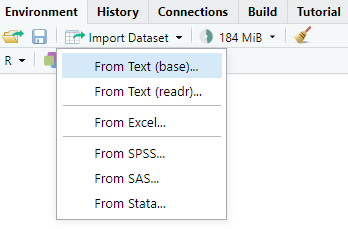
\includegraphics[width=3.125in,height=\textheight]{./images/import_01.PNG}

}

\caption{\label{fig-imp-01}Auf den Reiter \emph{Einviroment} klicken und
dann \emph{Import Dataset}. In der deutschen version vom RStudio mögen
die Begriffe leicht anders sein.}

\end{figure}

\begin{tcolorbox}[enhanced jigsaw, bottomrule=.15mm, toptitle=1mm, colbacktitle=quarto-callout-tip-color!10!white, opacityback=0, bottomtitle=1mm, leftrule=.75mm, toprule=.15mm, breakable, rightrule=.15mm, title=\textcolor{quarto-callout-tip-color}{\faLightbulb}\hspace{0.5em}{Importieren mit RStudio als Video}, coltitle=black, colframe=quarto-callout-tip-color-frame, colback=white, titlerule=0mm, left=2mm, arc=.35mm, opacitybacktitle=0.6]
Du findest auf YouTube \href{https://youtu.be/tdRWkBcGAzk}{Einführung in
R - Teil 21.0 - Daten importieren mit RStudio - Point and Klick} als
Video. Point and Klick ist als Video einfacher nachzuvollziehen als
Screenshots in einem Fließtext.
\end{tcolorbox}

\hypertarget{sec-pfad}{%
\section{Importieren per Pfad}\label{sec-pfad}}

In Abbildung~\ref{fig-imp-02} können wir sehen wie wir den Pfad zu
unserer Excel Datei \texttt{flea\_dog\_cat.xlsx} finden. Natürlich
kannst du den Pfad auch anders herausfinden bzw. aus dem Explorer oder
Finder kopieren.

\begin{figure}

{\centering 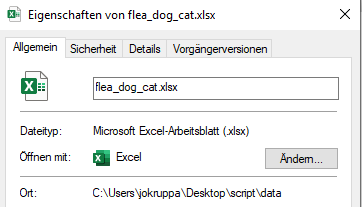
\includegraphics[width=3.64583in,height=\textheight]{./images/import_02.PNG}

}

\caption{\label{fig-imp-02}Durch den Rechts-Klick auf die Eigenschaften
einer Datei kann man sich den Pfad zur Datei anzeigen lassen.
\textbf{Achtung!} Unter Windows muss der Slash \texttt{\textbackslash{}}
noch in den Backslash \texttt{/} gedreht werden.}

\end{figure}

Nachdem wir den Pfad gefunden haben, können wir den Pfad in die Funktion
\texttt{read\_excel()} kopieren und die Datei in das Objekt
\texttt{data\_tbl} einlesen. Ja, es wird nichts in der R Console
ausgegeben, da sich die Daten jetzt in dem Object \texttt{data\_tbl}
befinden.

\begin{Shaded}
\begin{Highlighting}[]
\DocumentationTok{\#\# Ganzer Pfad zur Datei flea\_dog\_cat.xlsx}
\NormalTok{data\_tbl }\OtherTok{\textless{}{-}} \FunctionTok{read\_excel}\NormalTok{(}\StringTok{"data/flea\_dog\_cat.xlsx"}\NormalTok{)}
\end{Highlighting}
\end{Shaded}

\begin{tcolorbox}[enhanced jigsaw, bottomrule=.15mm, toptitle=1mm, colbacktitle=quarto-callout-important-color!10!white, opacityback=0, bottomtitle=1mm, leftrule=.75mm, toprule=.15mm, breakable, rightrule=.15mm, title=\textcolor{quarto-callout-important-color}{\faExclamation}\hspace{0.5em}{Unterschied zwischen \texttt{\textbackslash{}} in Windows und \texttt{/}
in R}, coltitle=black, colframe=quarto-callout-important-color-frame, colback=white, titlerule=0mm, left=2mm, arc=.35mm, opacitybacktitle=0.6]
Achte einmal auf den Slash im Pfad in R und einem im Pfsd in Windows.
Einmal ist es der Slash \texttt{\textbackslash{}} im Dateipfad und
einmal der Backslash \texttt{/}. Das ist sehr ärgerlich, aber dieses
Problem geht zurück in die 80'ziger. Bill hat entschieden für sein
Windows \texttt{/} zu nutzen und Steve (und Unix) eben \texttt{/}. Und
mit dieser Entscheidung müssen wir jetzt leben\ldots{}
\end{tcolorbox}

\hypertarget{sec-umlaute}{%
\section{Auf ein englisches Wort in Dateien}\label{sec-umlaute}}

Ein großes Problem in Datein sind Umlaute (ä,ö,ü) oder aber andere
(Sonder)zeichen (ß, ?, oder \#). Als dies sollte vermieden werden. Eine
gute Datei für R beinhaltet nur \emph{ganze} Wörter, Zahlen oder aber
leere Felder. Ein leeres Feld ist ein fehlender Wert.
Abbildung~\ref{fig-imp-03} zeigt eine gute Exceldatentablle. Wir
schreiben \texttt{jump\_length} mit Unterstrich um den Namen besser zu
lesen zu können. Sonst ist auch alles in Englisch geschrieben. Wir
vermeiden durch die neglische Schreibweise \emph{aus versehen} einen
Umlaut oder anderweitig problematische Zeichen zu verwenden. Später
können wir alles noch für Abbildungen anpassen.

\begin{figure}

{\centering 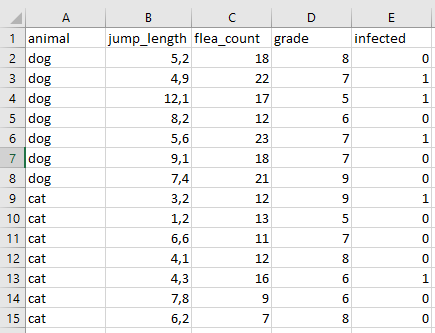
\includegraphics{./images/import_03.PNG}

}

\caption{\label{fig-imp-03}Beispiel für eine gute (Excel)Datentabelle.
Keine Umlaute sind vorhanden und die Spaltennamen haben keine
Leerzeichen oder Sonderzeichen.}

\end{figure}

\hypertarget{sec-spalten}{%
\section{Spaltennamen in der (Excel)-Datei}\label{sec-spalten}}

Die Funktion \texttt{clean\_names()} aus dem R Paket \texttt{janitor}
erlaubt es die Spaltennamen einer eingelesenen Datei in eine für R gute
Form zu bringen.

\begin{itemize}
\tightlist
\item
  Keine Leerzeichen in den Spaltennamen.
\item
  Alle Spaltennamen sind klein geschrieben.
\end{itemize}

\begin{Shaded}
\begin{Highlighting}[]
\NormalTok{data\_tbl }\SpecialCharTok{\%\textgreater{}\%} 
  \FunctionTok{clean\_names}\NormalTok{()}
\end{Highlighting}
\end{Shaded}

\begin{verbatim}
# A tibble: 14 x 5
   animal jump_length flea_count grade infected
   <chr>        <dbl>      <dbl> <dbl>    <dbl>
 1 dog            5.7         18     8        0
 2 dog            8.9         22     8        1
 3 dog           11.8         17     6        1
 4 dog            8.2         12     8        0
 5 dog            5.6         23     7        1
 6 dog            9.1         18     7        0
 7 dog            7.6         21     9        0
 8 cat            3.2         12     7        1
 9 cat            2.2         13     5        0
10 cat            5.4         11     7        0
11 cat            4.1         12     6        0
12 cat            4.3         16     6        1
13 cat            7.9          9     6        0
14 cat            6.1          7     5        0
\end{verbatim}

\hypertarget{sec-dplyr}{%
\chapter{Daten bearbeiten}\label{sec-dplyr}}

Wir haben in dem vorherigen Kapitel Daten eingelesen. Jetzt wollen wir
die Daten aufräumen (eng. \emph{tidy}). Es ist notwendig, dass wir die
Daten so aufarbeiten, dass R damit umgehen kann. Insbesondere das
Erstellen von Faktoren ist wichtig, wenn die Spalte ein Faktor ist. R
muss wissen was für Eigenschaften eine Spalte hat. Sonst funktionieren
spätere Anwendungen in R nicht richtig oder geben einen Fehler wieder.

Es gibt zwei Möglichkeiten wie du mit deinen Daten umgehst:

\begin{enumerate}
\def\labelenumi{\arabic{enumi})}
\tightlist
\item
  Du änderst all deine Daten in Excel. Das mag bei einem kleinen
  Datensatz gut funktionieren. Dann musst du dich nicht mit dem
  \emph{Programmieren} beschäftigen.
\item
  Du willst lernen die Daten auch in R zu verändern. Dann hilft dir
  dieses Kapitel. Auch in den folgenden Kapiteln werde ich immer wieder
  Funktionen wie \texttt{select()}, \texttt{filter()} und
  \texttt{mutate()}nutzen. Dann kannst du hier nochmal schauen, was die
  Funktionen machen.
\end{enumerate}

Im Folgenden wollen wir den Datensatz \texttt{data\_tbl} in R
bearbeiten. Das heißt wir wollen Spalten auswählen mit \texttt{select()}
oder Zeilen auswählen mit \texttt{filter()}. Schlussendlich wollen wir
auch die Eigenschaften von Spalten mit der Funktion \texttt{mutate}
ändern. Wir laden also den Datensatz \texttt{flea\_dog\_cat.xlsx} einmal
in R.

\begin{Shaded}
\begin{Highlighting}[]
\NormalTok{data\_tbl }\OtherTok{\textless{}{-}} \FunctionTok{read\_excel}\NormalTok{(}\StringTok{"data/flea\_dog\_cat\_fox.xlsx"}\NormalTok{)}
\end{Highlighting}
\end{Shaded}

Es ergibt sich folgende Tabelle~\ref{tbl-dog-cat-dplyr}, die wir schon
aus vorherigen Kapiteln kennen.

\hypertarget{tbl-dog-cat-dplyr}{}
\begin{longtable}[]{@{}ccccc@{}}
\caption{\label{tbl-dog-cat-dplyr}Tabelle der Sprunglängen {[}cm{]},
Anzahl an Flöhen, Boniturnote sowie der Infektionsstatus von Hunden,
Katzen und Füchsen.}\tabularnewline
\toprule()
animal & jump\_length & flea\_count & grade & infected \\
\midrule()
\endfirsthead
\toprule()
animal & jump\_length & flea\_count & grade & infected \\
\midrule()
\endhead
dog & 5.7 & 18 & 8 & 0 \\
dog & 8.9 & 22 & 8 & 1 \\
dog & 11.8 & 17 & 6 & 1 \\
dog & 8.2 & 12 & 8 & 0 \\
dog & 5.6 & 23 & 7 & 1 \\
dog & 9.1 & 18 & 7 & 0 \\
dog & 7.6 & 21 & 9 & 0 \\
cat & 3.2 & 12 & 7 & 1 \\
cat & 2.2 & 13 & 5 & 0 \\
cat & 5.4 & 11 & 7 & 0 \\
cat & 4.1 & 12 & 6 & 0 \\
cat & 4.3 & 16 & 6 & 1 \\
cat & 7.9 & 9 & 6 & 0 \\
cat & 6.1 & 7 & 5 & 0 \\
fox & 7.7 & 21 & 5 & 1 \\
fox & 8.1 & 25 & 4 & 1 \\
fox & 9.1 & 31 & 4 & 1 \\
fox & 9.7 & 12 & 5 & 1 \\
fox & 10.6 & 28 & 4 & 0 \\
fox & 8.6 & 18 & 4 & 1 \\
fox & 10.3 & 19 & 3 & 0 \\
\bottomrule()
\end{longtable}

\hypertarget{genutzte-r-pakete-fuxfcr-das-kapitel-1}{%
\section{Genutzte R Pakete für das
Kapitel}\label{genutzte-r-pakete-fuxfcr-das-kapitel-1}}

Wir wollen folgende R Pakete in diesem Kapitel nutzen.

\begin{Shaded}
\begin{Highlighting}[]
\NormalTok{pacman}\SpecialCharTok{::}\FunctionTok{p\_load}\NormalTok{(tidyverse, readxl, magrittr, janitor)}
\end{Highlighting}
\end{Shaded}

Am Ende des Kapitels findest du nochmal den gesamten R Code in einem
Rutsch zum selber durchführen oder aber kopieren.

\hypertarget{spalten-wuxe4hlen-mit-select}{%
\section{\texorpdfstring{Spalten wählen mit
\texttt{select()}}{Spalten wählen mit select()}}\label{spalten-wuxe4hlen-mit-select}}

\begin{tcolorbox}[enhanced jigsaw, bottomrule=.15mm, toptitle=1mm, colbacktitle=quarto-callout-tip-color!10!white, opacityback=0, bottomtitle=1mm, leftrule=.75mm, toprule=.15mm, breakable, rightrule=.15mm, title=\textcolor{quarto-callout-tip-color}{\faLightbulb}\hspace{0.5em}{YouTube - Spalten auswählen mit select()}, coltitle=black, colframe=quarto-callout-tip-color-frame, colback=white, titlerule=0mm, left=2mm, arc=.35mm, opacitybacktitle=0.6]
Du findest auf YouTube \href{https://youtu.be/oV_7A2nMIrM}{Einführung in
R - Teil 12 - Spalten auswählen mit select()} als Video zum nochmal
anschauen.
\end{tcolorbox}

{\marginnote{\begin{footnotesize}Wir nutzen die Funktion
\texttt{select()}um Spalten zu wählen.\end{footnotesize}}}

Der Datensatz, den wir im Experiment erschaffen, ist meist riesig. Jetzt
könnten wir natürlich eine Exceltabelle mit unterschiedlichen Sheets
bzw. Reitern erstellen oder aber die \emph{Spalten} die wir brauchen in
R selektieren. Wir nutzen die Funktion \texttt{select()}um Spalten zu
wählen. Im folgenden Codeblock wählen wir die Spalten \texttt{animal},
\texttt{jump\_length} und \texttt{flea\_count}.

\begin{Shaded}
\begin{Highlighting}[]
\NormalTok{data\_tbl }\SpecialCharTok{\%\textgreater{}\%} 
  \FunctionTok{select}\NormalTok{(animal, jump\_length, flea\_count)}
\end{Highlighting}
\end{Shaded}

\begin{verbatim}
# A tibble: 21 x 3
   animal jump_length flea_count
   <chr>        <dbl>      <dbl>
 1 dog            5.7         18
 2 dog            8.9         22
 3 dog           11.8         17
 4 dog            8.2         12
 5 dog            5.6         23
 6 dog            9.1         18
 7 dog            7.6         21
 8 cat            3.2         12
 9 cat            2.2         13
10 cat            5.4         11
# ... with 11 more rows
\end{verbatim}

Wir können die Spalten beim selektieren auch umbenennen und in eine
andere Reihenfolge bringen.

\begin{Shaded}
\begin{Highlighting}[]
\NormalTok{data\_tbl }\SpecialCharTok{\%\textgreater{}\%} 
  \FunctionTok{select}\NormalTok{(}\AttributeTok{Sprungweite =}\NormalTok{ jump\_length, flea\_count, animal)}
\end{Highlighting}
\end{Shaded}

\begin{verbatim}
# A tibble: 21 x 3
   Sprungweite flea_count animal
         <dbl>      <dbl> <chr> 
 1         5.7         18 dog   
 2         8.9         22 dog   
 3        11.8         17 dog   
 4         8.2         12 dog   
 5         5.6         23 dog   
 6         9.1         18 dog   
 7         7.6         21 dog   
 8         3.2         12 cat   
 9         2.2         13 cat   
10         5.4         11 cat   
# ... with 11 more rows
\end{verbatim}

Du findest auf der englischen
\href{https://dplyr.tidyverse.org/reference/select.html}{Hilfeseite für
select()} noch weitere Beispiele für die Nutzung.

\hypertarget{zeilen-wuxe4hlen-mit-filter}{%
\section{\texorpdfstring{Zeilen wählen mit
\texttt{filter()}}{Zeilen wählen mit filter()}}\label{zeilen-wuxe4hlen-mit-filter}}

\begin{tcolorbox}[enhanced jigsaw, bottomrule=.15mm, toptitle=1mm, colbacktitle=quarto-callout-tip-color!10!white, opacityback=0, bottomtitle=1mm, leftrule=.75mm, toprule=.15mm, breakable, rightrule=.15mm, title=\textcolor{quarto-callout-tip-color}{\faLightbulb}\hspace{0.5em}{YouTube - Zeilen auswählen mit filter()}, coltitle=black, colframe=quarto-callout-tip-color-frame, colback=white, titlerule=0mm, left=2mm, arc=.35mm, opacitybacktitle=0.6]
Du findest auf YouTube \href{https://youtu.be/Pw_KnGWZjpM}{Einführung in
R - Teil 13 - Zeilen auswählen mit filter()} als Video zum nochmal
anschauen.
\end{tcolorbox}

{\marginnote{\begin{footnotesize}Wir nutzen die Funktion
\texttt{filter()} um Zeilen nach Kriterien zu
wählen.\end{footnotesize}}}

Während wir die Auswahl an Spalten gut und gerne auch in Excel
durchführen können, so ist dies bei der Auswahl der Zeilen nicht so
einfach. Wir können in R hier auf die Funktion \texttt{filter()}
zurückgreifen. Wir nutzen die Funktion \texttt{filter()} um Zeilen nach
Kriterien zu wählen.

Im folgenden Codeblock wählen wir die Zeilen aus in denen die Worte
\texttt{dog} und \texttt{fox} stehen. Wir nutzen dazu den Operator
\texttt{\%in\%} um auszudrücken, dass wir alle Einträge in der Spalte
\texttt{animal} wollen die in dem Vektor \texttt{c("dog",\ "fox")}
beschrieben sind.

\begin{Shaded}
\begin{Highlighting}[]
\NormalTok{data\_tbl }\SpecialCharTok{\%\textgreater{}\%} 
  \FunctionTok{filter}\NormalTok{(animal }\SpecialCharTok{\%in\%} \FunctionTok{c}\NormalTok{(}\StringTok{"dog"}\NormalTok{, }\StringTok{"fox"}\NormalTok{))}
\end{Highlighting}
\end{Shaded}

\begin{verbatim}
# A tibble: 14 x 5
   animal jump_length flea_count grade infected
   <chr>        <dbl>      <dbl> <dbl>    <dbl>
 1 dog            5.7         18     8        0
 2 dog            8.9         22     8        1
 3 dog           11.8         17     6        1
 4 dog            8.2         12     8        0
 5 dog            5.6         23     7        1
 6 dog            9.1         18     7        0
 7 dog            7.6         21     9        0
 8 fox            7.7         21     5        1
 9 fox            8.1         25     4        1
10 fox            9.1         31     4        1
11 fox            9.7         12     5        1
12 fox           10.6         28     4        0
13 fox            8.6         18     4        1
14 fox           10.3         19     3        0
\end{verbatim}

Es stehen dir Folgende logische Operatoren zu Verfügung wie in
Tabelle~\ref{tbl-logical-operators} gezeigt. Am Anfang ist es immer
etwas schwer sich in den logischen Operatoren zurechtzufinden. Daher
kann ich dir nur den Tipp geben einmal die Operatoren selber
auszuprobieren und zu schauen, was du da so rausfilterst.

\hypertarget{tbl-logical-operators}{}
\begin{longtable}[]{@{}
  >{\raggedright\arraybackslash}p{(\columnwidth - 2\tabcolsep) * \real{0.2927}}
  >{\raggedright\arraybackslash}p{(\columnwidth - 2\tabcolsep) * \real{0.7073}}@{}}
\caption{\label{tbl-logical-operators}Logische Opertairen und R und
deren Beschreibung}\tabularnewline
\toprule()
\begin{minipage}[b]{\linewidth}\raggedright
\textbf{Logischer Operator}
\end{minipage} & \begin{minipage}[b]{\linewidth}\raggedright
\textbf{Beschreibung}
\end{minipage} \\
\midrule()
\endfirsthead
\toprule()
\begin{minipage}[b]{\linewidth}\raggedright
\textbf{Logischer Operator}
\end{minipage} & \begin{minipage}[b]{\linewidth}\raggedright
\textbf{Beschreibung}
\end{minipage} \\
\midrule()
\endhead
\textbf{\textless{}} & kleiner als (eng. \emph{less than}) \\
\textbf{\textless=} & kleiner als oder gleich (eng. \emph{less than or
equal to}) \\
\textbf{\textgreater{}} & größer als (eng. \emph{greater than}) \\
\textbf{\textgreater=} & größer als oder gleich (eng. \emph{greater than
or equal to}) \\
\textbf{==} & exact gleich (eng. \emph{exactly equal to}) \\
\textbf{!=} & nicht gleich (eng. \emph{not equal to}) \\
\textbf{!x} & nicht (eng. \emph{not x}) \\
\textbf{x \textbar{} y} & oder (eng. \emph{x or y}) \\
\textbf{x \& y} & und (eng. \emph{x and y}) \\
\bottomrule()
\end{longtable}

Hier ein paar Beispiele. Probiere gerne auch mal Operatoren selber aus.
Im folgenden Codeblock wollen wir nur die Zeilen haben, die eine Anzahl
an Flöhen größer von 15 haben.

\begin{Shaded}
\begin{Highlighting}[]
\NormalTok{data\_tbl }\SpecialCharTok{\%\textgreater{}\%} 
  \FunctionTok{filter}\NormalTok{(flea\_count }\SpecialCharTok{\textgreater{}} \DecValTok{15}\NormalTok{)}
\end{Highlighting}
\end{Shaded}

\begin{verbatim}
# A tibble: 13 x 5
   animal jump_length flea_count grade infected
   <chr>        <dbl>      <dbl> <dbl>    <dbl>
 1 dog            5.7         18     8        0
 2 dog            8.9         22     8        1
 3 dog           11.8         17     6        1
 4 dog            5.6         23     7        1
 5 dog            9.1         18     7        0
 6 dog            7.6         21     9        0
 7 cat            4.3         16     6        1
 8 fox            7.7         21     5        1
 9 fox            8.1         25     4        1
10 fox            9.1         31     4        1
11 fox           10.6         28     4        0
12 fox            8.6         18     4        1
13 fox           10.3         19     3        0
\end{verbatim}

Wir wollen nur die infizierten Tiere haben.

\begin{Shaded}
\begin{Highlighting}[]
\NormalTok{data\_tbl }\SpecialCharTok{\%\textgreater{}\%} 
  \FunctionTok{filter}\NormalTok{(infected }\SpecialCharTok{==} \ConstantTok{TRUE}\NormalTok{)}
\end{Highlighting}
\end{Shaded}

\begin{verbatim}
# A tibble: 10 x 5
   animal jump_length flea_count grade infected
   <chr>        <dbl>      <dbl> <dbl>    <dbl>
 1 dog            8.9         22     8        1
 2 dog           11.8         17     6        1
 3 dog            5.6         23     7        1
 4 cat            3.2         12     7        1
 5 cat            4.3         16     6        1
 6 fox            7.7         21     5        1
 7 fox            8.1         25     4        1
 8 fox            9.1         31     4        1
 9 fox            9.7         12     5        1
10 fox            8.6         18     4        1
\end{verbatim}

Wir wollen nur die infizierten Tiere haben UND die Tiere mit einer
Flohanzahl größer als 20.

\begin{Shaded}
\begin{Highlighting}[]
\NormalTok{data\_tbl }\SpecialCharTok{\%\textgreater{}\%} 
  \FunctionTok{filter}\NormalTok{(infected }\SpecialCharTok{==} \ConstantTok{TRUE} \SpecialCharTok{\&}\NormalTok{ flea\_count }\SpecialCharTok{\textgreater{}} \DecValTok{20}\NormalTok{)}
\end{Highlighting}
\end{Shaded}

\begin{verbatim}
# A tibble: 5 x 5
  animal jump_length flea_count grade infected
  <chr>        <dbl>      <dbl> <dbl>    <dbl>
1 dog            8.9         22     8        1
2 dog            5.6         23     7        1
3 fox            7.7         21     5        1
4 fox            8.1         25     4        1
5 fox            9.1         31     4        1
\end{verbatim}

Du findest auf der englischen
\href{https://dplyr.tidyverse.org/reference/filter.html\%3E}{Hilfeseite
für filter()} noch weitere Beispiele für die Nutzung.

\hypertarget{spalten-uxe4ndern-mit-mutate}{%
\section{\texorpdfstring{Spalten ändern mit
\texttt{mutate()}}{Spalten ändern mit mutate()}}\label{spalten-uxe4ndern-mit-mutate}}

\begin{tcolorbox}[enhanced jigsaw, bottomrule=.15mm, toptitle=1mm, colbacktitle=quarto-callout-tip-color!10!white, opacityback=0, bottomtitle=1mm, leftrule=.75mm, toprule=.15mm, breakable, rightrule=.15mm, title=\textcolor{quarto-callout-tip-color}{\faLightbulb}\hspace{0.5em}{YouTube - Eigenschaften von Variablen ändern mit mutate()}, coltitle=black, colframe=quarto-callout-tip-color-frame, colback=white, titlerule=0mm, left=2mm, arc=.35mm, opacitybacktitle=0.6]
Du findest auf YouTube \href{https://youtu.be/P6eum3wy9Ek}{Einführung in
R - Teil 14 - Eigenschaften von Variablen ändern mit mutate()} als Video
zum nochmal anschauen.
\end{tcolorbox}

\marginnote{\begin{footnotesize}

Wir nutzen die Funktion \texttt{mutate()} um die Eigenschaften von
Spalten daher Variablen zu ändern.

Die Reihenfolge der Funktionen ist wichtig um unliebsame Effekte zu
vermeiden.

\begin{enumerate}
\def\labelenumi{\arabic{enumi})}
\tightlist
\item
  Erst wählen wir die Spalten mit \texttt{select()}
\item
  Dann filtern wir die Zeilen mit \texttt{filter()}
\item
  Abschließend ändern wir die Eigenschaften der Spalten mit
  \texttt{mutate()}
\end{enumerate}

\end{footnotesize}}

Nachdem wir die Spalten mit \texttt{select()} udn eventuell die Zeieln
mit \texttt{filter()} gewählt haben. müssen wir jetzt noch die
Eigenschaften der Spalten ändern. Das Ändern müssen wir nicht immer tun,
aber häufig müssen wir noch einen Faktor erschaffen. Wir nutzen noch die
Funktion \texttt{pull()} um uns die Spalte \texttt{animal} aus dem
Datensatz zu ziehen. Nur so sehen wir die vollen Eigenschaften des
Faktors. Später nutzen wir \texttt{pull} seltener und nur um zu
kontrollieren, was wir gemacht haben.

Im folgenden Codeblock verwandeln wir die Variable \texttt{animal} in
einen Faktor durch die Funktion \texttt{as\_factor}. Wir sehen, dass die
Level des Faktoes so sortiert sind, wie das Auftreten in der Spalte
\texttt{animal}.

\begin{Shaded}
\begin{Highlighting}[]
\NormalTok{data\_tbl }\SpecialCharTok{\%\textgreater{}\%} 
  \FunctionTok{mutate}\NormalTok{(}\AttributeTok{animal =} \FunctionTok{as\_factor}\NormalTok{(animal)) }\SpecialCharTok{\%\textgreater{}\%} 
  \FunctionTok{pull}\NormalTok{(animal)}
\end{Highlighting}
\end{Shaded}

\begin{verbatim}
 [1] dog dog dog dog dog dog dog cat cat cat cat cat cat cat fox fox fox fox fox
[20] fox fox
Levels: dog cat fox
\end{verbatim}

Wollen wir die Sortierung der Level ändern, können wir die Funktion
\texttt{factor()} nutzen. Wir ändern die Sortierung des Faktors zu
\texttt{fox}, \texttt{dog} und \texttt{cat}.

\begin{Shaded}
\begin{Highlighting}[]
\NormalTok{data\_tbl }\SpecialCharTok{\%\textgreater{}\%} 
  \FunctionTok{mutate}\NormalTok{(}\AttributeTok{animal =} \FunctionTok{factor}\NormalTok{(animal, }\AttributeTok{levels =} \FunctionTok{c}\NormalTok{(}\StringTok{"fox"}\NormalTok{, }\StringTok{"dog"}\NormalTok{, }\StringTok{"cat"}\NormalTok{))) }\SpecialCharTok{\%\textgreater{}\%} 
  \FunctionTok{pull}\NormalTok{(animal)}
\end{Highlighting}
\end{Shaded}

\begin{verbatim}
 [1] dog dog dog dog dog dog dog cat cat cat cat cat cat cat fox fox fox fox fox
[20] fox fox
Levels: fox dog cat
\end{verbatim}

Wir können auch die Namen (eng. \emph{labels}) der Level ändern. Hier
musst du nur aufpassen wie du die alten Labels überschreibst. Wenn ich
\emph{gleichzeitig} die Level und die Labels ändere komme ich häufig
durcheinander. Da muss du eventuell nochmal schauen, ob auch alles so
geklappt hat wie du wolltest.

\begin{Shaded}
\begin{Highlighting}[]
\NormalTok{data\_tbl }\SpecialCharTok{\%\textgreater{}\%} 
  \FunctionTok{mutate}\NormalTok{(}\AttributeTok{animal =} \FunctionTok{factor}\NormalTok{(animal, }\AttributeTok{labels =} \FunctionTok{c}\NormalTok{(}\StringTok{"Hund"}\NormalTok{, }\StringTok{"Katze"}\NormalTok{, }\StringTok{"Fuchs"}\NormalTok{))) }\SpecialCharTok{\%\textgreater{}\%} 
  \FunctionTok{pull}\NormalTok{(animal)}
\end{Highlighting}
\end{Shaded}

\begin{verbatim}
 [1] Katze Katze Katze Katze Katze Katze Katze Hund  Hund  Hund  Hund  Hund 
[13] Hund  Hund  Fuchs Fuchs Fuchs Fuchs Fuchs Fuchs Fuchs
Levels: Hund Katze Fuchs
\end{verbatim}

Du findest auf der englischen
\href{https://dplyr.tidyverse.org/reference/mutate.html}{Hilfeseite für
mutate()} noch weitere Beispiele für die Nutzung. Insbesondere die
Nutzung von \texttt{mutate()} über mehrere Spalten gleichzeitig erlaubt
sehr effiezientes Programmieren. Aber das ist für den Anfang etwas viel.

\begin{tcolorbox}[enhanced jigsaw, bottomrule=.15mm, toptitle=1mm, colbacktitle=quarto-callout-note-color!10!white, opacityback=0, bottomtitle=1mm, leftrule=.75mm, toprule=.15mm, breakable, rightrule=.15mm, title=\textcolor{quarto-callout-note-color}{\faInfo}\hspace{0.5em}{Die Funktionen select(), filter() und mutate() in R}, coltitle=black, colframe=quarto-callout-note-color-frame, colback=white, titlerule=0mm, left=2mm, arc=.35mm, opacitybacktitle=0.6]
Bitte schaue dir auch die Hilfeseiten der Funktionen an. In diesem
Skript kann ich nicht alle Funktionalitäten der Funktionen zeigen. Oder
du kommst in das R Tutorium welches ich anbiete und fragst dort nach den
Möglichkeiten Daten in R zu verändern.
\end{tcolorbox}

\hypertarget{gruppieren-mit-group_by}{%
\section{\texorpdfstring{Gruppieren mit
\texttt{group\_by()}}{Gruppieren mit group\_by()}}\label{gruppieren-mit-group_by}}

Sobald wir einen Faktor erschaffen haben, können wir die Daten in R auch
nach dem Faktor \emph{gruppieren}. Das heißt wir nutzen die Funktion
\texttt{group\_by()} um R mitzuteilen, dass nun folgende Funktionen
\emph{getrennt} für die einzelen Gruppen erfolgen sollen. Im folgenden
Codeblock siehst du die Anwendung.

\begin{Shaded}
\begin{Highlighting}[]
\NormalTok{data\_tbl }\SpecialCharTok{\%\textgreater{}\%} 
  \FunctionTok{mutate}\NormalTok{(}\AttributeTok{animal =} \FunctionTok{as\_factor}\NormalTok{(animal)) }\SpecialCharTok{\%\textgreater{}\%} 
  \FunctionTok{group\_by}\NormalTok{(animal)}
\end{Highlighting}
\end{Shaded}

\begin{verbatim}
# A tibble: 21 x 5
# Groups:   animal [3]
   animal jump_length flea_count grade infected
   <fct>        <dbl>      <dbl> <dbl>    <dbl>
 1 dog            5.7         18     8        0
 2 dog            8.9         22     8        1
 3 dog           11.8         17     6        1
 4 dog            8.2         12     8        0
 5 dog            5.6         23     7        1
 6 dog            9.1         18     7        0
 7 dog            7.6         21     9        0
 8 cat            3.2         12     7        1
 9 cat            2.2         13     5        0
10 cat            5.4         11     7        0
# ... with 11 more rows
\end{verbatim}

Auf den ersten Blick ändert sich nicht viel. Es entsteht aber die Zeile
\texttt{\#\ Groups:\ animal\ {[}3{]}}. Wir wissen nun, dass wir nach der
Variable \texttt{animal} mit drei Gruppen die Datentabelle gruppiert
haben. Die Anwendung siehst du in Kapitel~\ref{sec-desc-group-by} bei
der Berechung von deskriptiven Maßzahlen.

\hypertarget{mehr-informationen-durch-glimpse-und-str}{%
\section{\texorpdfstring{Mehr Informationen durch \texttt{glimpse()} und
\texttt{str()}}{Mehr Informationen durch glimpse() und str()}}\label{mehr-informationen-durch-glimpse-und-str}}

Am Ende noch zwei Funktionen zur Kontrolle, was wir hier eigentlich
gerade tun. Mit der Funktion \texttt{glimpse()} können wir uns einen
Einblick in die Daten geben lassen. Wir sehen dann nochmal kurz und
knapp wieviel Zeieln und Spalten wir haben und welche Inhalte in den
Spalten stehen. Die gleichen Informationen erhalten wir auch durch die
Funktion \texttt{str()}. Die Funktion \texttt{str()}geht aber noch einen
Schritt weiter und nennt uns auch Informationen zu dem Objekt. Daher wir
wissen jetzt, dass es sich beim dem Objekt \texttt{data\_tbl} um ein
\texttt{tibble()} handelt.

\begin{Shaded}
\begin{Highlighting}[]
\FunctionTok{glimpse}\NormalTok{(data\_tbl)}
\end{Highlighting}
\end{Shaded}

\begin{verbatim}
Rows: 21
Columns: 5
$ animal      <chr> "dog", "dog", "dog", "dog", "dog", "dog", "dog", "cat", "c~
$ jump_length <dbl> 5.7, 8.9, 11.8, 8.2, 5.6, 9.1, 7.6, 3.2, 2.2, 5.4, 4.1, 4.~
$ flea_count  <dbl> 18, 22, 17, 12, 23, 18, 21, 12, 13, 11, 12, 16, 9, 7, 21, ~
$ grade       <dbl> 8, 8, 6, 8, 7, 7, 9, 7, 5, 7, 6, 6, 6, 5, 5, 4, 4, 5, 4, 4~
$ infected    <dbl> 0, 1, 1, 0, 1, 0, 0, 1, 0, 0, 0, 1, 0, 0, 1, 1, 1, 1, 0, 1~
\end{verbatim}

\begin{Shaded}
\begin{Highlighting}[]
\FunctionTok{str}\NormalTok{(data\_tbl)}
\end{Highlighting}
\end{Shaded}

\begin{verbatim}
tibble [21 x 5] (S3: tbl_df/tbl/data.frame)
 $ animal     : chr [1:21] "dog" "dog" "dog" "dog" ...
 $ jump_length: num [1:21] 5.7 8.9 11.8 8.2 5.6 9.1 7.6 3.2 2.2 5.4 ...
 $ flea_count : num [1:21] 18 22 17 12 23 18 21 12 13 11 ...
 $ grade      : num [1:21] 8 8 6 8 7 7 9 7 5 7 ...
 $ infected   : num [1:21] 0 1 1 0 1 0 0 1 0 0 ...
\end{verbatim}

\part{Explorative Datenanalyse}

{\marginnote{\begin{footnotesize}Wir kürzen die \textbf{e}xplorative
\textbf{D}aten\textbf{a}nalyse häufig als \textbf{EDA}
ab.\end{footnotesize}}}

Wir haben die Daten jetzt in R Eingelesen und im Zweifel noch angepasst.
Nun wollen wir uns die Daten einmal angucken. Nicht in dem Sinne, dass
wir auf die Daten\emph{tabelle} schauen. Sondern wir wollen die Daten
visualisieren. Wir erstellen Abbildungen von den Daten und versuchen so
mehr über die Daten zu erfahren. Sehen wir Zusammenhänge zwischen
verschiedenen Variablen bzw. Spalten? Wir führen eine explorative
Datenanalyse durch. Über die exploratibve Datenanalyse wollen wir uns in
diesem Kapitel einmal Gedanken machen.

\begin{tcolorbox}[enhanced jigsaw, bottomrule=.15mm, toptitle=1mm, colbacktitle=quarto-callout-tip-color!10!white, opacityback=0, bottomtitle=1mm, leftrule=.75mm, toprule=.15mm, breakable, rightrule=.15mm, title=\textcolor{quarto-callout-tip-color}{\faLightbulb}\hspace{0.5em}{Einführung in R per Video}, coltitle=black, colframe=quarto-callout-tip-color-frame, colback=white, titlerule=0mm, left=2mm, arc=.35mm, opacitybacktitle=0.6]
Du findest auf YouTube
\href{https://www.youtube.com/playlist?list=PLe51bCp9JvEFUnFqaJG5aRmON9i1ZbOYC}{Grundlagen
in R} als Video Reihe. Du musst die Grundlagen in R verstanden haben,
damit du dem R Code folgen kannst.
\end{tcolorbox}

\hypertarget{sec-desc-stat}{%
\chapter{Deskriptive Statistik}\label{sec-desc-stat}}

{\marginnote{\begin{footnotesize}Eigentlich \emph{schätzen} wir die
\textbf{Parameter einer Verteilung}. Aber das kommt nochmal später
genauer, wenn wir wissen was Verteilungen sind.\end{footnotesize}}}

Wir nutzen die deskriptive Statistik um Zahlen zusammenzufassen. Das
heißt wir haben einen Datensatz vorliegen wie den Datensatz
\texttt{flea\_dog\_cat.xlsx}. Wir wollen jetzt den großen Datensatz in
wenige Zahlen wiedergeben. Warum wenige Zahlen? Wenn wir das Ergebnis
\emph{präsentieren} wollen, dann müssen es wenige Zahlen sein, die den
Datensatz gut zusammenfassen. Daher ist es wichtig zu wissen, dass wir
\emph{dutzende bis hunderte Zahlen} durch meist eine oder zwei Zahlen
beschreiben wollen. Wir brauchen die statistischen Maßzahlen aus diesem
Kapitel später um teilweise noch extrem größere Datensätze darstellen zu
können. Ebenso werden wir die Maßzahlen aus diesem Kapitel dafür
verwenden statistische Tests und Modelle zu rechnen.

Nehmen wir nun als Beispiel die Sprungweiten in {[}cm{]} von
Hundeflöhen. Wir messen sieben Sprungweiten von sieben Hundeflöhen und
messen dabei folgende Werte in {[}cm{]}: 5.7, 8.9, 11.8, 8.2, 5.6, 9.1
und 7.6. Wir schreiben nun y als einen Vektor in der Form

\[
y = \{5.7, 8.9, 11.8, 8.2, 5.6, 9.1, 7.6\}.
\]

In R würde der Vektor wie etwas anders aussehen.

\begin{Shaded}
\begin{Highlighting}[]
\NormalTok{y }\OtherTok{\textless{}{-}} \FunctionTok{c}\NormalTok{(}\FloatTok{5.7}\NormalTok{, }\FloatTok{8.9}\NormalTok{, }\FloatTok{11.8}\NormalTok{, }\FloatTok{8.2}\NormalTok{, }\FloatTok{5.6}\NormalTok{, }\FloatTok{9.1}\NormalTok{, }\FloatTok{7.6}\NormalTok{) }
\end{Highlighting}
\end{Shaded}

Wir wollen nun die Zahlen in \(y\) beschrieben und durch wenige andere
Zahlen zusammenfassen. Einige der statistischen Maßzahlen sind dir
vermutlich schon bekannt, andere eher neu.

\begin{tcolorbox}[enhanced jigsaw, bottomrule=.15mm, toptitle=1mm, colbacktitle=quarto-callout-note-color!10!white, opacityback=0, bottomtitle=1mm, leftrule=.75mm, toprule=.15mm, breakable, rightrule=.15mm, title=\textcolor{quarto-callout-note-color}{\faInfo}\hspace{0.5em}{Parametrik versus Nicht-Parametrik}, coltitle=black, colframe=quarto-callout-note-color-frame, colback=white, titlerule=0mm, left=2mm, arc=.35mm, opacitybacktitle=0.6]

Wenn wir einen Zahlenvektor wie durch
\(y = \{5.7, 8.9, 11.8, 8.2, 5.6, 9.1, 7.6\}\) beschrieben
zusammenfassen wollen, haben wir zwei Möglichkeiten.

\begin{enumerate}
\def\labelenumi{\arabic{enumi})}
\tightlist
\item
  Die \textbf{parametrische Variante} indem wir \emph{mit den Zahlen}
  rechnen und deskriptive Maßzahlen wie Mittelwert, Varianz und
  Standardabweichung berechnen. Diese Maßzahlen kommen aber in den
  Zahlen nicht vor.
\item
  Die \textbf{nicht-parametrische} Variante indem wir die Zahlen in
  Ränge umwandeln, also sortieren, und \emph{mit den Rängen} der Zahlen
  rechnen. Die deskriptiven Maßzahlen wären dann Median, Quantile und
  Quartile.
\end{enumerate}

\end{tcolorbox}

\hypertarget{mittelwert}{%
\section{Mittelwert}\label{mittelwert}}

Der Mittelwert einer Zahlenreihe beschreibt den Schwerpunkt der Zahlen.
Der Mittelwert wird auch als Lageparameter benannt.
{\marginnote{\begin{footnotesize}Der \textbf{Mittelwert} und der
\textbf{Median} sind zwei Lageparameter einer Verteilung. Beide
beschreiben die Stelle, wo die Verteilungskurve am höchsten
ist.\end{footnotesize}}} Wir schreiben den Mittelwert mit einem Strich
über den Vektor, der die Zahlen enthält. Im folgenden ist die Formel für
den Mittelwert der Sprungweite in {[}cm{]} der Hunde gezeigt. Der
Mittelwert ist in dem Sinne eine künstliche Zahl, da der Mittlwert
häufig nicht in den beobachteten Zahlen vorkommt.

\begin{marginfigure}

{\centering 
\includegraphics[width=0.5\textwidth,height=\textheight]{./images/angel_01.png}

}

\end{marginfigure}

Wir werden immer mal wieder \textbf{Formeln vereinfachen}. Zum Beispiel
nur \(\sum\) schreiben anstatt \(\sum_i^n\), wenn wir einen Vektor
aufsummieren und uns die Indizes sparen\ldots{}

\[
\bar{y} = \sum_{i=1}^{n}\cfrac{x_i}{n} =
\cfrac{5.7 + 8.9 + 11.8 + 8.2 + 5.6 + 9.1 + 7.6}{7} =
8.13
\]

Im Durchschnitt oder im Mittel springen Hundeflöhe 8.13 cm weit.

In der Abbildung~\ref{fig-index-drawn} wollen wir die Formel nochmal
visualisieren. Vielleicht fällt dir dann der Zusammenhang von dem Index
\(i\) und der gesamten Fallzahl \(n\) leichter.

\begin{figure}

{\centering 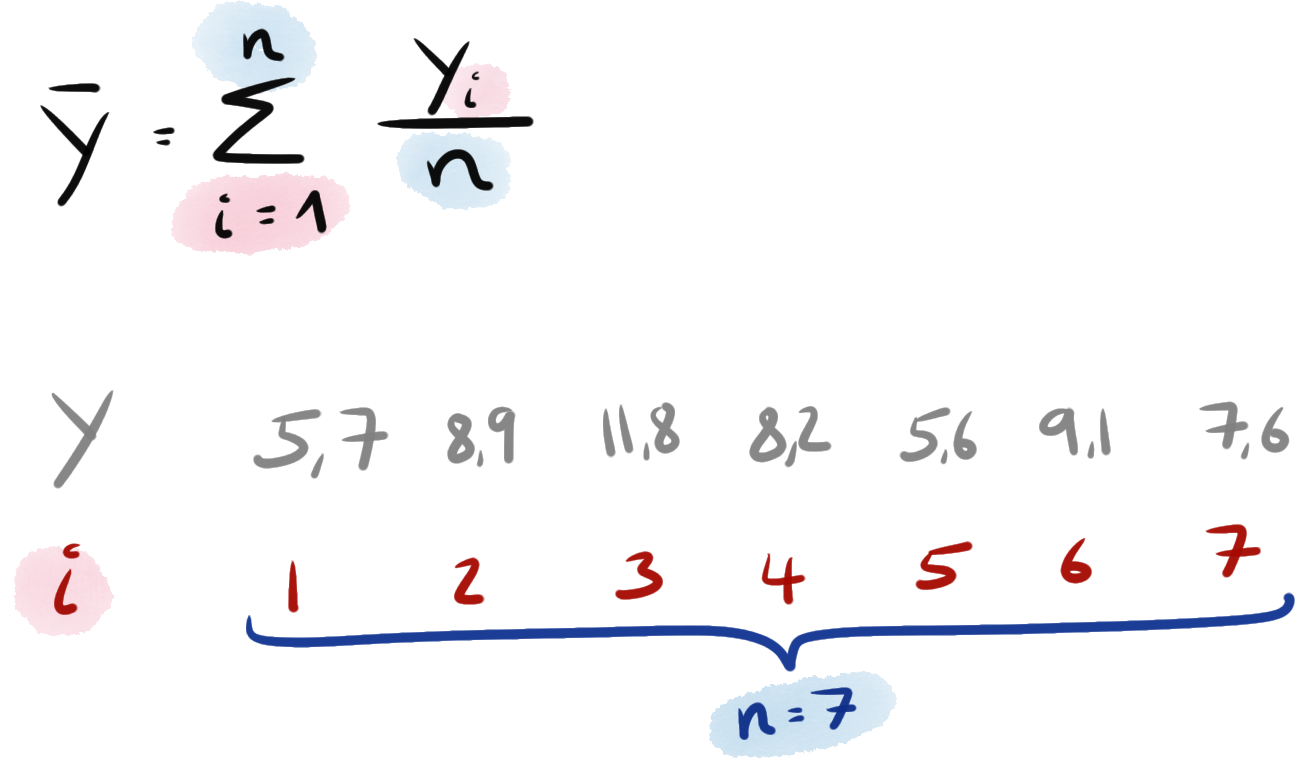
\includegraphics[width=1\textwidth,height=\textheight]{./images/index-drawn.png}

}

\caption{\label{fig-index-drawn}Zusamenhang zwischen \(y\) sowie dem
Index \(i\) in der Formel für den Mittelwert.}

\end{figure}

In R können wir den Mittelwert einfach mit der Funktion \texttt{mean()}
berechnen. Wir wollen dann den Mittelwert noch auf die zweite
Kommastelle runden. Das machen wir dann mit der Funktion
\texttt{round()}.

\begin{Shaded}
\begin{Highlighting}[]
\NormalTok{y }\SpecialCharTok{\%\textgreater{}\%}\NormalTok{ mean }\SpecialCharTok{\%\textgreater{}\%} \FunctionTok{round}\NormalTok{(}\DecValTok{2}\NormalTok{)}
\end{Highlighting}
\end{Shaded}

\begin{verbatim}
[1] 8.13
\end{verbatim}

Wir erhalten das gleiche Ergebnis wie oben in unserer händischen
Rechnung. Die Hundeflöhe springen im Mittel 8.13 cm weit.

Der Mittelwert ist eine bedeutende Maßzahl der Normalverteilung. Daher
merken wir uns hier schon mal, dass wir den Mittelwert brauchen werden.
Auch wenn wir darüber nachdenken ob sich zwei Gruppen unterscheiden, so
nutzen wir hierzu den Mitelwert. Unterscheiden sich die \emph{mittleren}
Sprungweiten in {[}cm{]} von Hunde- und Katzenflöhen?

\hypertarget{spannweite}{%
\section{Spannweite}\label{spannweite}}

Die \emph{Spannweite} erlaubt uns zu überprüfen was die kleinste Zahl
und die größte Zahl ist. Also uns das Minimum und das Maximum einer
Zahlenreihe anzuschauen. Auf den ersten Blick mag das nicht so sinnig
sein, aber wenn wir uns hunderte von Beobachtungen anschauen, wollen wir
wissen, ob wir nicht einen Fehler bei Eintragen der Daten gemacht haben.
Wir wissen eigentlich, dass z.B keine negativen Zuwachsraten auftreten
können.

{\marginnote{\begin{footnotesize}Die Spannweite dient dazu in einem
Datensatz zu übersprüfen ob die \textbf{Spalte}, oder auch
\textbf{Variable} genannt, den richtigen Zahlenraum aufweist. Das machen
wir durch die Funktion \texttt{range()}.\end{footnotesize}}}

\[
y_{range} = y_{max} - y_{min} = 12.1 - 4.9 = 7.2
\] Die Hundeflöhe springen in einer Spannweite von 7.2 cm. Das kommt
einem \emph{normal} vor. Die Spannweite ist nicht übertrieben groß. Der
minimale Wert ist 4.9 und der maximale Wert it 12.1 und somit sind beide
Zahlen in Ordnung. Keine der beiden Zahlen ist übertrieben groß oder gar
negativ.

In R können wir die Spannweite mit \texttt{range()} wie folgt berechnen.
Wir erhalten den minmialen udn maximalen Wert.

\begin{Shaded}
\begin{Highlighting}[]
\FunctionTok{range}\NormalTok{(y) }
\end{Highlighting}
\end{Shaded}

\begin{verbatim}
[1]  5.6 11.8
\end{verbatim}

Wir merken uns, dass die Spannweite eine Maßzahl für die Validität der
Daten ist. Hat das Experiment geklappt oder kamen da nur komische Zahlen
bei raus, die wir so in der Realität nicht erwarten würden. Zum Beispiel
negative Sprungweiten, weil wir einmalauf das Minuszeichen gekommen
sind.

\hypertarget{varianz}{%
\section{Varianz}\label{varianz}}

Bis jetzt können wirmit dem Mittelwert \(\bar{y}\) die Lage oder den
Mittelpunkt unserer Zahlenreihe beschreiben. Uns fehlt damit aber die
Information über die Streuung der Zahlen. Sind die Zahlen alle eher
gleich oder sehr verschieden? Liegen die Zahlen daher alle bei dem
Mittelwert oder sind die Zahlen weit um den Mittelwert gestreut.

Die Streuung der Zahlen um den Mittelwert beschreibt die Varianz oder
auch \(s^2\). Wir berechnen die Varianz indem wir von jeder Zahl den
Mittelwert aller Zahlen abziehen und dann das Ergebnis quadrieren. Das
machen wir für alle Zahlen und addieren dann die Summe auf. Wir erhalten
die \emph{Quadratsumme} von \(y\).

{\marginnote{\begin{footnotesize}\textbf{Abweichungsquadrate} sind ein
wichtiges Konzept in der Statistik. Wenn wir wissen wollen, wie groß
eine Abweichung von einer Zahl zu einer anderen ist, dann nutzen wir
immer das Quadrat der Abweichung und bilden die
Quadratsumme..\end{footnotesize}}}

\[
s^2 = \sum_{i=1}^n\cfrac{(y_i - \bar{y})^2}{n-1} = \cfrac{(5.7 -
8.13)^2 + ... + (7.6 - 8.13)^2}{7-1} = 4.6
\]

Die Varianz berschreibt also die Streuung der Zahlen \emph{im Quadrat}
um den Mittelwert. Das heißt in unserem Beispiel, dass die Sprungweite
eine Varianz von 4.6 cm\(^2\) hat. Wir können Quadratzentimeter schlecht
interpretieren. Deshalb führen wir gleich die Wuzel der Varianz ein: die
Standardabweichung.

In R lässt sich die Varianz einfach durch die Funktion \texttt{var()}
berechnen.

\begin{Shaded}
\begin{Highlighting}[]
\NormalTok{y }\SpecialCharTok{\%\textgreater{}\%}\NormalTok{ var }\SpecialCharTok{\%\textgreater{}\%} \FunctionTok{round}\NormalTok{(}\DecValTok{2}\NormalTok{) }
\end{Highlighting}
\end{Shaded}

\begin{verbatim}
[1] 4.6
\end{verbatim}

Wir benötigen die Varianz häufig nur als Zwischenschritt um die
Standardabweichung zu berechnen. Das Konzept der Abweichungsquadrate
benötigen wir aber in der Varianzanalyse (ANOVA) und für die
Beschreibung einer Normalverteilung.

\hypertarget{standardabweichung}{%
\section{Standardabweichung}\label{standardabweichung}}

Die \emph{Standardabweichugn} ist die Wurzel der Varianz. Wo die Varianz
die Abweichung der Sprungweite in {[}cm\(^2\){]} beschreibt, beschreibt
die Standardabweichung die Streung der Sprungweite in {[}cm{]}.

\[
s = \sqrt{s^2} = \sqrt{4.6} = 2.14
\] {\marginnote{\begin{footnotesize}Wir schreiben immer den Mittelwert
plusminus die Standardabweichung. Also immer
\(\bar{y} \pm s\).\end{footnotesize}}}

Wir können also schreiben, dass die Flöhe im Mittel 8.13 \(\pm\) 2.14cm
weit springen. Somit haben wir die Lage und die Streuung der Zahlenreihe
\(y\) der Sprungweite in {[}cm{]} mit zwei Zahlen beschrieben.

In R können wir die Standardabweichung einfach mit der Funktion
\texttt{sd()} berechnen.

\begin{Shaded}
\begin{Highlighting}[]
\NormalTok{y }\SpecialCharTok{\%\textgreater{}\%}\NormalTok{ sd }\SpecialCharTok{\%\textgreater{}\%} \FunctionTok{round}\NormalTok{(}\DecValTok{2}\NormalTok{) }
\end{Highlighting}
\end{Shaded}

\begin{verbatim}
[1] 2.14
\end{verbatim}

\hypertarget{mittelwert-und-varianz---eine-herleitung}{%
\section{Mittelwert und Varianz - eine
Herleitung}\label{mittelwert-und-varianz---eine-herleitung}}

Was ist der Mitelwert und die Varianz genau? Schauen wir uns das einmal
in Abbildung~\ref{fig-mean-drawn} an. Die graue Linie oder Grade
beschreibt den Mittelwert der fünf Beobachtungen. Die fünf Beobachtungen
sind als blaue Punkt dargestellt. Auf der x-Achse ist nur der Index des
Punktes. Das heißt \(y_1\) ist der erste Punkte, das der Index \(i\)
gleich 1 ist.

\begin{figure}

{\centering 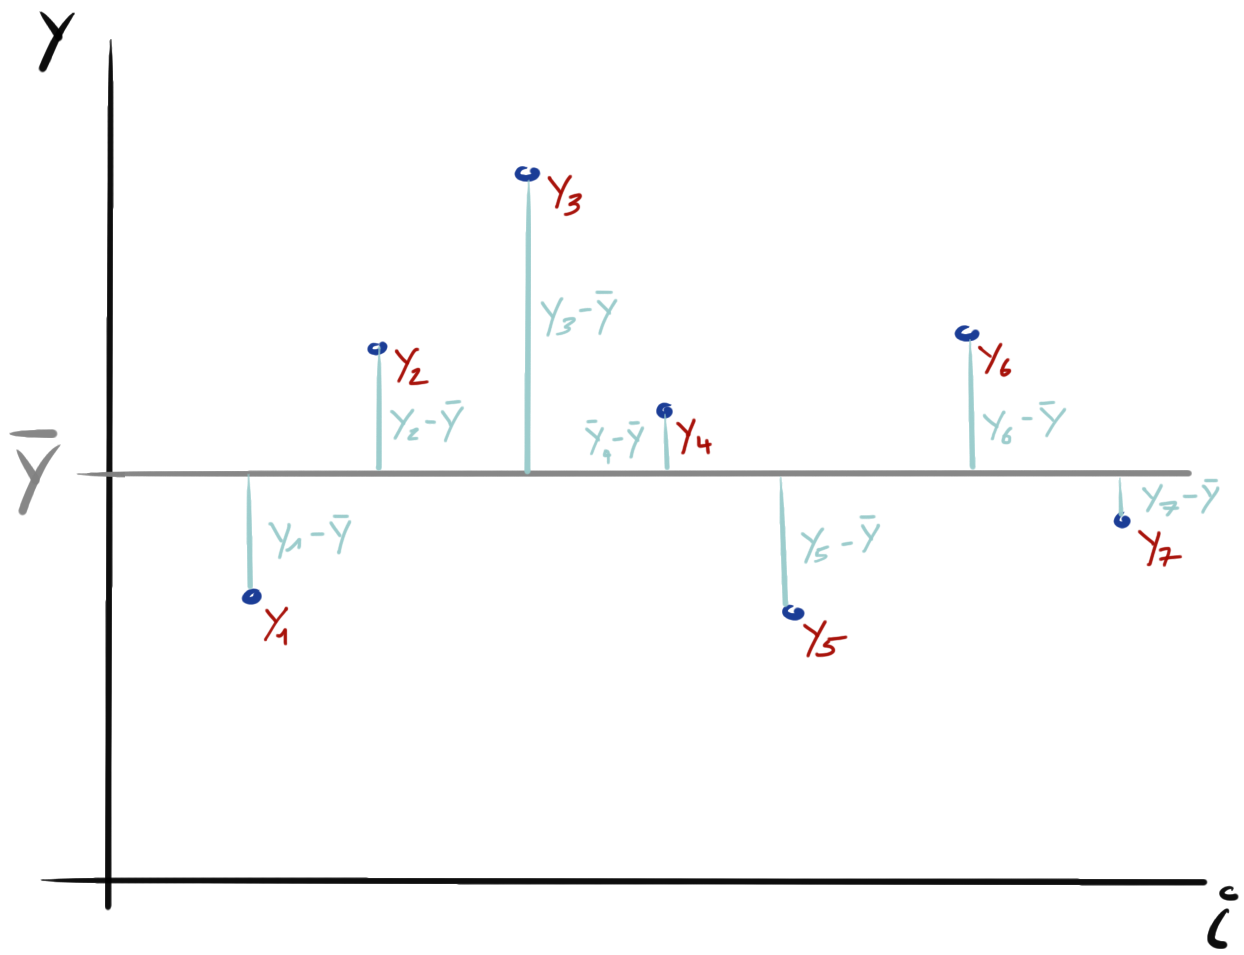
\includegraphics[width=1\textwidth,height=\textheight]{./images/mean-drawn.png}

}

\caption{\label{fig-mean-drawn}Die graue Linie beschreibt den Mittelwert
der genau so durch die blauen Punkte geht, dass die Abstände der Punkte
oberhalb und unterhalb zu Null aufaddieren. Die Linie liegt in der Mitte
der Punkte. Die quadrierten Abstände sind die Varainz der blauen Punkte.
Auf der x-Achse ist der Index des Punktes eingetragen.}

\end{figure}

Wenn wir die Summe der Abweichungen von \(y_1\) bis \(y_5\) zu dem
Mittelwert bilden, so wird diese Summe 0 sein. Der Mittelwert liegt
genau in der Mitte der Punkte. In unserem Beispiel ist der Mittelwert
\(\bar{y} = 5.8\). Wi können jetzt die Abstände wie in der folgenden
Tabelle berechnen.

\begin{figure*}

\begin{longtable}[]{@{}
  >{\centering\arraybackslash}p{(\columnwidth - 8\tabcolsep) * \real{0.1170}}
  >{\centering\arraybackslash}p{(\columnwidth - 8\tabcolsep) * \real{0.0638}}
  >{\centering\arraybackslash}p{(\columnwidth - 8\tabcolsep) * \real{0.2660}}
  >{\centering\arraybackslash}p{(\columnwidth - 8\tabcolsep) * \real{0.3191}}
  >{\centering\arraybackslash}p{(\columnwidth - 8\tabcolsep) * \real{0.2340}}@{}}
\toprule()
\begin{minipage}[b]{\linewidth}\centering
Index \(i\)
\end{minipage} & \begin{minipage}[b]{\linewidth}\centering
y
\end{minipage} & \begin{minipage}[b]{\linewidth}\centering
\(\boldsymbol{\epsilon}\)
\end{minipage} & \begin{minipage}[b]{\linewidth}\centering
\(\boldsymbol{y_i - \bar{y}}\)
\end{minipage} & \begin{minipage}[b]{\linewidth}\centering
Wert
\end{minipage} \\
\midrule()
\endhead
1 & 5.7 & \(\epsilon_1\) & \(y_1 - \bar{y}\) & \(5.7 - 8.13 = -2.43\) \\
2 & 8.9 & \(\epsilon_2\) & \(y_2 - \bar{y}\) & \(8.9 - 8.13 = 0.77\) \\
3 & 11.8 & \(\epsilon_3\) & \(y_3 - \bar{y}\) &
\(11.8 - 8.13 = 3.67\) \\
4 & 8.2 & \(\epsilon_4\) & \(y_4 - \bar{y}\) & \(8.2 - 8.13 = 0.07\) \\
5 & 5.6 & \(\epsilon_5\) & \(y_5 - \bar{y}\) & \(5.6 - 8.13 = -2.53\) \\
6 & 9.1 & \(\epsilon_4\) & \(y_4 - \bar{y}\) & \(9.1 - 8.13 = 0.97\) \\
7 & 7.6 & \(\epsilon_5\) & \(y_5 - \bar{y}\) & \(7.6 - 8.13 = -0.53\) \\
\bottomrule()
\end{longtable}

\end{figure*}

Wir nennen die Abstände \(y_i - \bar{y}\) nach dem griechischen
Buchstaben Epsilon \(\epsilon\). Das \(\epsilon\) soll an das \(e\) von
\emph{Error} erinnern. So meint dann \emph{Error} eben auch Abweichung.
Ja, es gibt hier viele Worte für das gleiche Konzept.

Wir berechnen einen Mittelwert von den Epsilons mit
\(\bar{\epsilon} = 0\). Ein Mittelwert nahe Null bzw. von Null wundert
uns nicht. Wir haben die Gerade ja so gebaut, das nach oben und unten
die gleichen Abstände sind. Die Varianz \(s^2\) der \(y\) ist
\(s_y^2 = 4.599\) und die Varianz von \(\epsilon\) ist
\(s_{\epsilon}^2 = 4.599\). In beiden Fällen ist die Zahl gleich. Wir
können uns merken, dass die Epsilons einen Mittelwert von 0 haben und
eine Varianz von \(s_y^2\).

{\marginnote{\begin{footnotesize}Wir schreiben auch, dass die Residuen
genannt \(\epsilon\) normalverteilt sind mit
\(\mathcal{N}(0, s_y^2)\).\end{footnotesize}}}

\hypertarget{standardfehler-oder-standard-error-se}{%
\section{Standardfehler oder Standard Error
(SE)}\label{standardfehler-oder-standard-error-se}}

Wenn wir den Mittelwert der Sprungweiten berichten dann gehört die
Standardabweichung der Sprungweiten mit als beschreibendes Maß dazu. Wir
berichten keinen Mittelwert ohne Standardabweichung.

Nun ist es aber so, dass der Mittelwert und die Standardabweichung von
der Fallzahl abhängen. Je mehr Fallzahl bzw. Beoabchtungen wir haben,
desto genauer wird der Mittelwert sein. Oder anders ausgedrückt
\(\bar{y}\) wird sich \(\mu_y\) annähern. Das gleiche gilt auch für die
Standardabweichung \(s_y\), die sich \(\sigma_y\) mit steigender
Fallzahl annähert.

Aus diesem Grund brauchen wir noch einen Fehler bzw. eine Maßzahl für
die Streuung, die unabhängig von der Fallzahl ist. Wir skalieren also
die Standardabweichung mit der Fallzahl indem wir die Standardbweichung
durch die Wurzel der Fallzahl teilen.

\[
SE = \cfrac{s}{\sqrt{n}} = \cfrac{2.14}{2.65} = 0.81
\]

Wir müssten ein Paket in R laden um den Standardfehler zu berechnen. Das
Laden von zusätzlichen Paketen wollen wir hier aber vermeiden; wir
können den Standardfehler auch einfach selber berechnen.

\begin{Shaded}
\begin{Highlighting}[]
\NormalTok{se }\OtherTok{\textless{}{-}} \FunctionTok{sd}\NormalTok{(y)}\SpecialCharTok{/}\FunctionTok{sqrt}\NormalTok{(}\FunctionTok{length}\NormalTok{(y))}
\NormalTok{se }\SpecialCharTok{\%\textgreater{}\%} \FunctionTok{round}\NormalTok{(}\DecValTok{2}\NormalTok{)}
\end{Highlighting}
\end{Shaded}

\begin{verbatim}
[1] 0.81
\end{verbatim}

Wir erhalten einen Standardfehler von 0.81. Diese Zahl ist in dem Sinne
nicht zu interpretieren, da wir hier nur Experimente losgelöst von deren
Fallzahl miteinander vergleichen können. Auf der anderen Seite können
wir ohne die berichtete Fallzahl nicht vom Standardfehler auf die
Standardabweichung schließen.

{\marginnote{\begin{footnotesize}Wir berichten den
\textbf{Standardfehler} immer zusammen mit der Fallzahl, so dass die
Standardabweichung berechnet werden kann.\end{footnotesize}}}

Wir benötigen den Standardfehler eigentlich nicht zum Berichten von
Ergebnissen. Der Standardfehler ist nicht als Zahl interpretierbar und
somit eine reine statistische Größe. Tabelle~\ref{tbl-comp-stand-sem}
zeigt die Zusammenfassung und den Vergleich von Standardabweichung und
Standardfehler.

\hypertarget{tbl-comp-stand-sem}{}
\begin{longtable}[]{@{}
  >{\raggedright\arraybackslash}p{(\columnwidth - 2\tabcolsep) * \real{0.5000}}
  >{\raggedright\arraybackslash}p{(\columnwidth - 2\tabcolsep) * \real{0.5000}}@{}}
\caption{\label{tbl-comp-stand-sem}Zusammenfassung und Vergleich von
Standardabweichung und Standardfehler}\tabularnewline
\toprule()
\begin{minipage}[b]{\linewidth}\raggedright
Standardabweichung
\end{minipage} & \begin{minipage}[b]{\linewidth}\raggedright
Standardfehler
\end{minipage} \\
\midrule()
\endfirsthead
\toprule()
\begin{minipage}[b]{\linewidth}\raggedright
Standardabweichung
\end{minipage} & \begin{minipage}[b]{\linewidth}\raggedright
Standardfehler
\end{minipage} \\
\midrule()
\endhead
\ldots{} ist eine Aussage über die Streuung der erhobenen Werte einer
Stichprobe. & \ldots{} ist eine Aussage über die Genauigkeit des
Mittelwertes einer Stichprobe. \\
\ldots{} hängt von der biologischen Variabilität ab. & \ldots{} abhängig
von der Messgenauigkeit \\
\ldots{} ist ein beschreibendes Maß. & \ldots{} ist ein statistisches
Maß. \\
\ldots{} ist nur wenig durch die Größe der Stichprobe beineinflussbar. &
\ldots{} steht im direkten Verhältnis zur Größe der Stichprobe. \\
\bottomrule()
\end{longtable}

\marginnote{\begin{footnotesize}

Der Standardfehler oder Standard Error (SE) oder Standard Error of the
Mean (SEM) wird uns wieder beim statistischen Testen und dem t-Test
begegnen.

\[
T_{calc} = \cfrac{\bar{y_1} - \bar{y_2}}{s_p \cdot \sqrt{\tfrac{2}{n}}} \approx \cfrac{\bar{y_1} - \bar{y_2}}{SEM}
\]

Der Nenner beim t-Test kann als Standardfehler gesehen werden. Wir
benötigen den Standardfehler also im Kontext des statistischen Testen
als eine statististische Maßzahl.

\end{footnotesize}}

\begin{tcolorbox}[enhanced jigsaw, bottomrule=.15mm, toptitle=1mm, colbacktitle=quarto-callout-note-color!10!white, opacityback=0, bottomtitle=1mm, leftrule=.75mm, toprule=.15mm, breakable, rightrule=.15mm, title=\textcolor{quarto-callout-note-color}{\faInfo}\hspace{0.5em}{Standardfehler wird in der Metaanalyse genutzt}, coltitle=black, colframe=quarto-callout-note-color-frame, colback=white, titlerule=0mm, left=2mm, arc=.35mm, opacitybacktitle=0.6]
Der Standardfehler ist bedeutend in der Metaanalyse. Also dem
gemeinsamen Auswerten von mehreren \emph{klinischen} Studien. Du kannst
im Buch
\href{https://bookdown.org/MathiasHarrer/Doing_Meta_Analysis_in_R/effects.html}{Doing
Meta-Analysis with R: A Hands-On Guide} mehr darüber erfahren. Wir
nutzen keine Metaanalysen in den Grundlagenveranstaltungen.
\end{tcolorbox}

\hypertarget{median}{%
\section{Median}\label{median}}

Wir wollen uns jetzt noch eine andere Art der Zusammenfassung von Zahlen
anschauen. Anstatt \emph{mit den Zahlen} zu rechnen, sortieren wir jetzt
die Zahlen aus dem Vektor \(y = \{5.7, 8.9, 11.8, 8.2, 5.6, 9.1, 7.6\}\)
nach dem Rang. Wir rechnen dann \emph{mit den Rängen}. Die kleinste Zahl
kriegt den kleinsten Rang. Wir können R nutzen über due Funktion
\texttt{sort()} um den Vektor \(y\) zu sortieren.

\begin{Shaded}
\begin{Highlighting}[]
\NormalTok{y }\SpecialCharTok{\%\textgreater{}\%} \FunctionTok{sort}\NormalTok{()}
\end{Highlighting}
\end{Shaded}

\begin{verbatim}
[1]  5.6  5.7  7.6  8.2  8.9  9.1 11.8
\end{verbatim}

Der Median \(\tilde{y}\) ist die mittlere Zahl eines Zahlenvektors. Wir
haben hier sieben Zahlen, also ist der Median die vierte Zahl. Wir
müssen hier aber zwischen einr ungeraden Anzahl und einer geraden Anzahl
unterscheiden.

\begin{itemize}
\tightlist
\item
  \textbf{Ungerade Anzahl} von Zahlen, der Median ist die mittlere Zahl
  des Vektors \(y\): \[
  5.6,  5.7,  7.6,  \underbrace{8.2,}_{Median}  8.9,  9.1, 11.8
  \]
\end{itemize}

In R können wir den Median einfach mit der Funktion
\texttt{median()}berechnen.

\begin{Shaded}
\begin{Highlighting}[]
\FunctionTok{median}\NormalTok{(y) }
\end{Highlighting}
\end{Shaded}

\begin{verbatim}
[1] 8.2
\end{verbatim}

\begin{itemize}
\tightlist
\item
  \textbf{Gerade Anzahl} von Zahlen, der Median ist der Mittelwert der
  \emph{beiden} mittleren Zahlen des Vektors \(y\): \[
  5.6,  5.7,  7.6,  \underbrace{8.2, 8.9,}_{Median = \tfrac{8.2+8.9}{2}=8.55} 9.1, 11.8, \color{blue}{13.1}
  \]
\end{itemize}

In R können wir den Median wieder einfach mit der Funktion
\texttt{median()}berechnen. Wir müssen nur die Zahl 13.1 zu dem Vektor
\texttt{y} mit der Funktion \texttt{c()} hinzufügen.

\begin{Shaded}
\begin{Highlighting}[]
\FunctionTok{c}\NormalTok{(y, }\FloatTok{13.1}\NormalTok{) }\SpecialCharTok{\%\textgreater{}\%} \FunctionTok{median}\NormalTok{() }
\end{Highlighting}
\end{Shaded}

\begin{verbatim}
[1] 8.55
\end{verbatim}

{\marginnote{\begin{footnotesize}Wenn der \textbf{Mittelwert} stark von
dem \textbf{Median} abweicht, deutet dies auf eine schiefe Verteilung
oder aber Ausreißer in den Daten hin. Wir müssen dann in der
explorativen Datenanalyse der Sachlage nachgehen\end{footnotesize}}}

Der Median ist eine Alternative zu dem Mitelwert. Insbesondere in
Fällen, wo es sehr große Zahlen gibt, die den Mittelwert in der Aussage
\emph{verzerren}, kann der Median sinnvoll sein.

\begin{tcolorbox}[enhanced jigsaw, bottomrule=.15mm, toptitle=1mm, colbacktitle=quarto-callout-tip-color!10!white, opacityback=0, bottomtitle=1mm, leftrule=.75mm, toprule=.15mm, breakable, rightrule=.15mm, title=\textcolor{quarto-callout-tip-color}{\faLightbulb}\hspace{0.5em}{Median versus Mittelwert}, coltitle=black, colframe=quarto-callout-tip-color-frame, colback=white, titlerule=0mm, left=2mm, arc=.35mm, opacitybacktitle=0.6]
Zur Veranschaulichung des Unterschiedes zwischen Median und Mittelwert
nehmen wir die Mietpreise in New York. Der \emph{mittlere} Mietpreis für
eine 2-Zimmerwohnung in Manhattan liegt bei 5000\$ pro Monat. In den
\emph{mittleren} Mietpreis gehen aber auch die Mieten der Billionaires'
Row mit ein. Der \emph{mediane} Mietpreis liegt bei 4000\$. Die hohen
Mieten \emph{ziehen} den Mittelwert nach rechts.
\end{tcolorbox}

\hypertarget{quantile-und-quartile}{%
\section{Quantile und Quartile}\label{quantile-und-quartile}}

Bei dem Mittelwert beschreibt die Standardabweichung die Streuung der
Daten um den Mitelwert. Bei dem Median sind dies die \emph{Quartile}.
Die Quartile beschreiben die Streuung der Daten um den Median. Um die
Quartile bestimmen zu können, teilen wir die Daten in 100 Quantile. Du
kannst dir Quantile wie Prozente vorstellen. Wir schneiden die Daten
also in 100 Scheiben. Das geht natürlich erst wirklich, wenn wir hundert
Zahlen haben. Deshalb hilft man sich mit Qua\textbf{r}tilen - von
Quarta, ein Viertel - aus. Tabelle~\ref{tbl-quart-quant} zeigt den
Zusammenhang.

\hypertarget{tbl-quart-quant}{}
\begin{longtable}[]{@{}ccc@{}}
\caption{\label{tbl-quart-quant}Zusammenfassung und Vergleich von
Quantilen, Quartilen und Median}\tabularnewline
\toprule()
Quantile & Quartile & Median \\
\midrule()
\endfirsthead
\toprule()
Quantile & Quartile & Median \\
\midrule()
\endhead
25\% Quantile & 1\(^{st}\) Quartile & \\
50\% Quantile & 2\(^{nd}\) Quartile & Median \\
75\% Quantile & 3\(^{rd}\) Quartile & \\
\bottomrule()
\end{longtable}

Wir bestimmen die Quartile wie den Median. Wir müssen unterscheiden, ob
wir eine ungerade Anzahl an Zahlen oder eine gerade Anzahl an Zahlen
vorliegen haben.

\begin{itemize}
\item
  \textbf{Ungerade Anzahl} von Zahlen, das 1\(^{st}\) Quartile ist die
  mittlere Zahl des unteren Mittels und das 3\(^{rd}\) Quartile ist die
  mittlere Zahl des oberen Mittels des Vektors \(y\): \[
  5.6,  \underbrace{5.7,}_{1st\ Quartile}  7.6,  8.2,  8.9,  \underbrace{9.1,}_{3rd\ Quartile} 11.8
  \]
\item
  \textbf{Gerade Anzahl} von Zahlen, das 1\(^{st}\) Quartile ist der
  Mittelwert der beiden mittleren Zahl des unteren Mittels und das
  3\(^{rd}\) Quartile ist der Mitelwert der beiden mittleren Zahlen des
  oberen Mittels des Vektors \(y\): \[
  5.6,  \underbrace{5.7, 7.6,}_{1st\ Quartile = \tfrac{5.7+7.6}{2}=6.65}    8.2,  8.9,  \underbrace{9.1, 11.8}_{3rd\ Quartile = \tfrac{9.1+11.8}{2}=10.45} \color{blue}{13.1}
  \]
\end{itemize}

{\marginnote{\begin{footnotesize}Das \textbf{95\% Quantile} und das
\textbf{97.25\% Quantile} werden wir später nochmal im statistischen
Testen brauchen. Auch hier ist die Idee, dass wir die Daten in hundert
Teile schneiden und uns dann die extremen Zahlen
anschauen.\end{footnotesize}}}

In R können wir den Median einfach mit der Funktion \texttt{quantile()}
berechnen. Wir berechnen hier das 25\% Quantile also das 1\(^{st}\)
Quartile sowie das 50\% Quantile also den Median und das 75\% Quantile
also das 3\(^{rd}\) Quartile.

\begin{Shaded}
\begin{Highlighting}[]
\NormalTok{y }\SpecialCharTok{\%\textgreater{}\%} \FunctionTok{quantile}\NormalTok{(}\AttributeTok{probs =} \FunctionTok{c}\NormalTok{(}\FloatTok{0.25}\NormalTok{, }\FloatTok{0.5}\NormalTok{, }\FloatTok{0.75}\NormalTok{)) }\SpecialCharTok{\%\textgreater{}\%} \FunctionTok{round}\NormalTok{(}\DecValTok{2}\NormalTok{)}
\end{Highlighting}
\end{Shaded}

\begin{verbatim}
 25%  50%  75% 
6.65 8.20 9.00 
\end{verbatim}

\begin{Shaded}
\begin{Highlighting}[]
\FunctionTok{c}\NormalTok{(y, }\FloatTok{13.1}\NormalTok{) }\SpecialCharTok{\%\textgreater{}\%} \FunctionTok{quantile}\NormalTok{(}\AttributeTok{probs =} \FunctionTok{c}\NormalTok{(}\FloatTok{0.25}\NormalTok{, }\FloatTok{0.5}\NormalTok{, }\FloatTok{0.75}\NormalTok{)) }\SpecialCharTok{\%\textgreater{}\%} \FunctionTok{round}\NormalTok{(}\DecValTok{2}\NormalTok{) }
\end{Highlighting}
\end{Shaded}

\begin{verbatim}
 25%  50%  75% 
7.12 8.55 9.77 
\end{verbatim}

Warum unterscheiden sich die händisch berechneten Quartile von den
Quartilen aus R? Es gibt verschiedene Arten der Berechnung. In der
Klausur nutzen wir die Art und Weise wie die händische Berechnung hier
beschrieben ist. Später in der Anwendung nehmen wir die Werte, die R
ausgibt. Die Abweichungen sind so maginal, dass wir diese Abweichungen
in der praktischen Anwendung ignorieren wollen.

\hypertarget{interquartilesabstand-iqr}{%
\section{Interquartilesabstand (IQR)}\label{interquartilesabstand-iqr}}

Der Interquartilesabstand (IQR) beschreibt den Abstand zwischen dem
1\(^{st}\) Quartile und dem 3\(^{rd}\) Quartile. Daher ist der
Interquartilesabstand (IQR) ähnlich der Spannweite zwischen dem
maximalen und minimalen Wert. Wir benötigen das Interquartilesabstand
(IQR) in der explorativen Datenanalyse wenn wir einen Boxplot erstellen
wollen.

\[
IQR = 3^{rd}\,\mbox{Quartile} - 1^{st}\,\mbox{Quartile} = 9.1 - 5.7 = 3.4
\]

\hypertarget{sec-desc-group-by}{%
\section{Zusammenfassen von Daten per Faktor}\label{sec-desc-group-by}}

Gut und soll ich jetzt für jeden Faktorlevel überall den Mittelwert mit
\texttt{mean()} berechnen? Geht das nicht einfacher? Ja, geht es. Im
folgenden siehst du, wie du den verschiedene deskriptive Maßzahlen in
einem Rutsch berechnen kannst.

\begin{Shaded}
\begin{Highlighting}[]
\NormalTok{data\_tbl }\SpecialCharTok{\%\textgreater{}\%}
  \FunctionTok{mutate}\NormalTok{(}\AttributeTok{animal =} \FunctionTok{as\_factor}\NormalTok{(animal)) }\SpecialCharTok{\%\textgreater{}\%}
  \FunctionTok{group\_by}\NormalTok{(animal) }\SpecialCharTok{\%\textgreater{}\%}
  \FunctionTok{summarise}\NormalTok{(}\AttributeTok{mean =} \FunctionTok{mean}\NormalTok{(jump\_length),}
            \AttributeTok{sd =} \FunctionTok{sd}\NormalTok{(jump\_length),}
            \AttributeTok{median =} \FunctionTok{median}\NormalTok{(jump\_length),}
            \AttributeTok{quantiles =} \FunctionTok{quantile}\NormalTok{(jump\_length, }
                                 \AttributeTok{probs =} \FunctionTok{c}\NormalTok{(}\FloatTok{0.25}\NormalTok{, }\FloatTok{0.5}\NormalTok{, }\FloatTok{0.75}\NormalTok{))) }\SpecialCharTok{\%\textgreater{}\%} 
  \FunctionTok{mutate}\NormalTok{(}\FunctionTok{across}\NormalTok{(}\FunctionTok{where}\NormalTok{(is.numeric), round, }\DecValTok{2}\NormalTok{))}
\end{Highlighting}
\end{Shaded}

\begin{verbatim}
# A tibble: 6 x 5
# Groups:   animal [2]
  animal  mean    sd median quantiles
  <fct>  <dbl> <dbl>  <dbl>     <dbl>
1 dog     8.13  2.14    8.2      6.65
2 dog     8.13  2.14    8.2      8.2 
3 dog     8.13  2.14    8.2      9   
4 cat     4.74  1.9     4.3      3.65
5 cat     4.74  1.9     4.3      4.3 
6 cat     4.74  1.9     4.3      5.75
\end{verbatim}

\hypertarget{sec-eda-ggplot}{%
\chapter{Visualisierung von Daten}\label{sec-eda-ggplot}}

{\marginnote{\begin{footnotesize}Wir nennen eine Abbildung auch häufig
Plot. Das ist der englische Begriff und hat nichts in unserem Kontext
mit einer Fläche zu tun.\end{footnotesize}}}

Ein wichtiger Teil in der Analyse von Daten ist die Visualisierung. Wir
glauben keine Auswertung eines mathematischen Algorithmus, wenn wir
nicht die Bestätigung in einer Abbildung sehen. Daher ist die
Visualisierung die Grundlage für ein fundiertes, wissenschaftliches
Arbeiten. In diesem Kapitel stelle ich dir verschiedene Abbilungen vor,
die uns helfen werden zu Verstehen ob es einen Zusammenhang zwischen Y
und X gibt. Wir haben ein \(y\) vorliegen, was wir auf die y-Achse eines
Graphen legen und daneben dann mehrere Variablen bzw. Spalten die wir
\(x\) nennen. Eine der Variablen legen wir auf die x-Achse des Graphen.
Nach den anderen \(x\) färben wir die Abbildung ein.

\hypertarget{genutzte-r-pakete-fuxfcr-das-kapitel-2}{%
\section{Genutzte R Pakete für das
Kapitel}\label{genutzte-r-pakete-fuxfcr-das-kapitel-2}}

Wir wollen folgende R Pakete in diesem Kapitel nutzen.

\begin{Shaded}
\begin{Highlighting}[]
\NormalTok{pacman}\SpecialCharTok{::}\FunctionTok{p\_load}\NormalTok{(tidyverse, magrittr, readxl, ggmosaic, }
\NormalTok{               janitor, see)}
\end{Highlighting}
\end{Shaded}

Am Ende des Kapitels findest du nochmal den gesamten R Code in einem
Rutsch zum selber durchführen oder aber kopieren.

\hypertarget{grundlagen-in-ggplot}{%
\section{Grundlagen in ggplot()}\label{grundlagen-in-ggplot}}

{\marginnote{\begin{footnotesize}Im Gegensatz zu dem Pipe-Operator
\texttt{\%\textgreater{}\%} nutzt ggplot den Operator \texttt{+} um die
verschiedenen ggplot Funktionen (\texttt{geom\_}) miteinander zu
verbinden.\end{footnotesize}}}

Wir nutzen in R das R Paket \texttt{ggplot2} um unsere Daten zu
visualisieren. Die zentrale Idee von \texttt{ggplot2} ist, dass wir uns
eine Abbildung wie ein Sandwich bauen. Zuerst legen wir eine Scheibe
Brot hin und legen uns dann Scheibe für Scheibe weitere Schichten
übereinander. Oder die Idee eines Bildes, wo wir erst die Leinwand
definieren und dann Farbschicht über Farbschicht auftragen. Das Konzept
von \texttt{ggplot2}ist schlecht zu be\emph{schreiben} deshalb habe ich
auch noch zwei Videos hierfür gemacht. Um den Prozess von
\texttt{ggplot2} zu visualisieren\ldots{}

\begin{tcolorbox}[enhanced jigsaw, bottomrule=.15mm, toptitle=1mm, colbacktitle=quarto-callout-tip-color!10!white, opacityback=0, bottomtitle=1mm, leftrule=.75mm, toprule=.15mm, breakable, rightrule=.15mm, title=\textcolor{quarto-callout-tip-color}{\faLightbulb}\hspace{0.5em}{Grundlagen von ggplot() im Video}, coltitle=black, colframe=quarto-callout-tip-color-frame, colback=white, titlerule=0mm, left=2mm, arc=.35mm, opacitybacktitle=0.6]
Du findest auf YouTube \href{https://youtu.be/SGwSVzJ9C-s}{Einführung in
R - Teil 16.0 - Trockenübung ggplot2 simpel und einfach erklärt} als
Video.

Sowie auch auf YouTube \href{https://youtu.be/SRRQQO3DXtc}{Einführung in
R - Teil 16.1 - Abbildungen mit ggplot in R erstellen. Idee und Konzept
von ggplot} als Video. Also alles nochmal als Video - vielleicht
einfacher nachzuvollziehen als in einem Fließtext.
\end{tcolorbox}

Die Funktion \texttt{ggplot()} ist die zentrale Funktion, die die
Leinwand erschafft auf der wir dann verschiedene Schichten aufbringen
werden. Diese Schichten heißen \texttt{geom}. Es gibt nicht nur ein
\texttt{geom} sondern mehrere. Zum Beispiel das \texttt{geom\_boxplot}
für die Erstellung von Boxplots, das \texttt{geom\_histogram} für die
Erstellung von Histogrammen.
\href{https://ggplot2.tidyverse.org/reference/index.html}{Die Auswahl
ist riesig}. Die einzelnen Schichten werden dann über den Operator
\texttt{+} miteinander verbunden. Soviel erstmal zur Trockenübung.
Schauen wir uns das ganze einmal an einem Beispiel an.

\hypertarget{datenbeispiel}{%
\subsection{Datenbeispiel}\label{datenbeispiel}}

Wir importieren den Datensatz \texttt{flea\_cat\_dog.xlsx} und wollen
einzelne Variablen visualisieren. Wir kennen den Datensatz schon aus dem
Kapitel~\ref{sec-example-2}. Dennoch nochmal hier der Datensatz in
Tabelle~\ref{tbl-cat-dog-ggplot}.

\begin{Shaded}
\begin{Highlighting}[]
\NormalTok{flea\_dog\_cat\_tbl }\OtherTok{\textless{}{-}} \FunctionTok{read\_excel}\NormalTok{(}\StringTok{"data/flea\_dog\_cat.xlsx"}\NormalTok{) }\SpecialCharTok{\%\textgreater{}\%} 
  \FunctionTok{mutate}\NormalTok{(}\AttributeTok{animal =} \FunctionTok{as\_factor}\NormalTok{(animal))}
\end{Highlighting}
\end{Shaded}

{\marginnote{\begin{footnotesize}Spaltennamen sind in \textbf{Englisch}
und haben \textbf{keine Leerzeichen}. Die Funktion
\texttt{clean\_names()} aus dem R Paket \texttt{janitor} ist hier eine
Hilfe.\end{footnotesize}}}

Im folgenden ist es wichtig, dass du dir die Spaltennamen merkst. Wir
können nur die exakten, wortwörtlichen Spaltennamen verwenden. Sonst
erhalten wir einen Fehler. Deshalb haben wir auch keine Leerzeichen in
den Spaltennamen.

\hypertarget{tbl-cat-dog-ggplot}{}
\begin{longtable}[]{@{}ccccc@{}}
\caption{\label{tbl-cat-dog-ggplot}Beispieldatensatz für Eigenschaften
von Flöhen von zwei Tierarten.}\tabularnewline
\toprule()
animal & jump\_length & flea\_count & grade & infected \\
\midrule()
\endfirsthead
\toprule()
animal & jump\_length & flea\_count & grade & infected \\
\midrule()
\endhead
dog & 5.7 & 18 & 8 & 0 \\
dog & 8.9 & 22 & 8 & 1 \\
dog & 11.8 & 17 & 6 & 1 \\
dog & 8.2 & 12 & 8 & 0 \\
dog & 5.6 & 23 & 7 & 1 \\
dog & 9.1 & 18 & 7 & 0 \\
dog & 7.6 & 21 & 9 & 0 \\
cat & 3.2 & 12 & 7 & 1 \\
cat & 2.2 & 13 & 5 & 0 \\
cat & 5.4 & 11 & 7 & 0 \\
cat & 4.1 & 12 & 6 & 0 \\
cat & 4.3 & 16 & 6 & 1 \\
cat & 7.9 & 9 & 6 & 0 \\
cat & 6.1 & 7 & 5 & 0 \\
\bottomrule()
\end{longtable}

\hypertarget{erste-abbildung-in-ggplot}{%
\subsection{Erste Abbildung in
ggplot()}\label{erste-abbildung-in-ggplot}}

Der folgende R Code erstellt die Leinwand in der
Abbildung~\ref{fig-ggplot-1} für die folgende, zusätzliches Schichten
(\texttt{geom}).

\begin{Shaded}
\begin{Highlighting}[]
\FunctionTok{ggplot}\NormalTok{(}\AttributeTok{data =}\NormalTok{ flea\_dog\_cat\_tbl, }
       \FunctionTok{aes}\NormalTok{(}\AttributeTok{x =}\NormalTok{ animal , }\AttributeTok{y =}\NormalTok{ jump\_length))}
\end{Highlighting}
\end{Shaded}

Wir schauen uns einmal den Code im Detail an.

\begin{itemize}
\tightlist
\item
  \texttt{ggplot} ruft die Funktion auf. Die Funktion ist dafür da den
  Plot zu zeichnen.
\item
  \texttt{data\ =\ flea\_dog\_cat\_tbl} bennent den Datensatz aus dem
  der Plot gebaut werden soll.
\item
  \texttt{aes()}ist die Abkürzung für \emph{aesthetics} und beschreibt,
  was auf die x-Achse soll, was auf die y-Achse soll sowie ob es noch
  andere Faktoren in den Daten gibt.

  \begin{itemize}
  \tightlist
  \item
    \texttt{x} braucht den Spaltennamen für die Variable auf der
    x-Achse.
  \item
    \texttt{y} braucht den Spaltennamen für die Variable auf der
    y-Achse.
  \end{itemize}
\end{itemize}

{\marginnote{\begin{footnotesize}\textbf{Faktoren} meint hier andere
Gruppenvariablen. Variablen sind ein anderes Wort für Spalten. Also
Variablen die wir mit \texttt{as\_factor}erschaffen
haben.\end{footnotesize}}}

\begin{figure}

{\centering 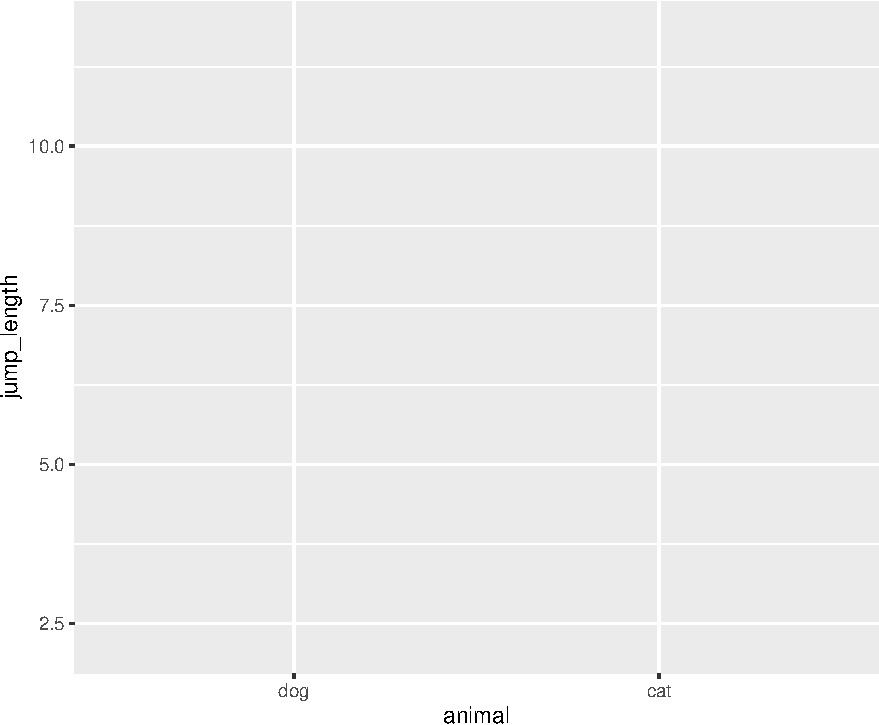
\includegraphics{./eda-ggplot_files/figure-pdf/fig-ggplot-1-1.pdf}

}

\caption{\label{fig-ggplot-1}Leere ggplot() Leinwand mit den Spalten
\texttt{animal} und \texttt{jump\_length} aus dem Datensatz
\texttt{flea\_dog\_cat\_tbl}.}

\end{figure}

Wir sehen, dass wir nichts sehen in Abbildung~\ref{fig-ggplot-1}. Der
Grund ist, dass wir noch kein \texttt{geom} hinzugefügt haben. Das
\texttt{geom} beschreibt nun wie die Zahlen in der Datentabelle
\texttt{flea\_dog\_cat\_tbl} visualisiert werden sollen.

\hypertarget{huxe4ufig-verwendete-abbildungen}{%
\section{Häufig verwendete
Abbildungen}\label{huxe4ufig-verwendete-abbildungen}}

In diesem Kapitel wollen wir durch die häufigsten und wichtigsten
Abbildungen in der explorativen Datenanalyse durchghen. Das wären im
folgenden diese Abbildungen:

\begin{itemize}
\tightlist
\item
  \textbf{Histogramm} in Kapitel~\ref{sec-eda-histogramm} für mehr als
  20 Beobachtungen (pro Gruppe). Wir nutzen ein Histogramm um die
  Verteilung einer Variable zu visualisieren.
\item
  \textbf{Boxplot} in Kapitel~\ref{sec-eda-boxplot} für 5 bis 20
  Beobachtungen (pro Gruppe). Ebenso wie bei einem Histogramm, geht es
  bei einem Boxplot auch um die Verteilung der einer Variable.
\item
  \textbf{Dotplot} in Kapitel~\ref{sec-eda-dotplot} für 3 bis 5
  Beobachtungen (pro Gruppe). Hier geht es weniger um die Verteilung der
  Variable, sondern darum die wenigen Beobachtungen zu visualisieren.
\item
  \textbf{Scatterplot} in Kapitel~\ref{sec-eda-scatter} für zwei
  kontinuierliche Variablen. Auch \textbf{xy-Plot} genannt. Die
  Abbildung, die dir bekannt sein müsste. Wir zeichnen hier eine Grade
  durch eine Punktewolke.
\item
  \textbf{Mosaicplot} in Kapitel~\ref{sec-eda-mosaic} für zwei diskrete
  Variablen. Eine etwas seltene Abbildung, wenn wir Variablen abbilden
  wollen, die diskret sind bzw. aus Kategorien bestehen.
\end{itemize}

{\marginnote{\begin{footnotesize}Konkret ist eine \textbf{Variable}
gleich einer \textbf{Spalte} in einem Datensatz.\end{footnotesize}}}

\begin{tcolorbox}[enhanced jigsaw, bottomrule=.15mm, toptitle=1mm, colbacktitle=quarto-callout-tip-color!10!white, opacityback=0, bottomtitle=1mm, leftrule=.75mm, toprule=.15mm, breakable, rightrule=.15mm, title=\textcolor{quarto-callout-tip-color}{\faLightbulb}\hspace{0.5em}{Histogramm, Boxplot, Scatterplot und Mosaicplot im Video}, coltitle=black, colframe=quarto-callout-tip-color-frame, colback=white, titlerule=0mm, left=2mm, arc=.35mm, opacitybacktitle=0.6]
Du findest auf YouTube \href{https://youtu.be/Zdw6NlLauNw}{Einführung in
R - Teil 16.2 - Histogramm, Boxplot, Scatterplot und Mosaicplot mit
ggplot in R} als Video. Weitere Videos werden dann noch folgen und
ergänzt.
\end{tcolorbox}

\hypertarget{sec-eda-histogramm}{%
\subsection{Histogramm}\label{sec-eda-histogramm}}

Wir nutzen für die Erstellung eines Histogramms den Datensatz
\texttt{dog\_fleas\_hist.csv}. Wir brauchen für ein anständiges
Histogramm, wo du auch was erkennen kannst, mindestens 20 Beobachtung.
Am besten mehr noch mhr Beobachtungen. Deshalb schauen wir uns jetzt
einmal 39 Hunde an und zählen wieviele Flöhe die Hunde jeweils haben,
dargestellt in der Spalte\texttt{flea\_count}. Darüber hinaus bestimmen
wir auch noch das mittlere Gewicht der Flöhe auf dem jeweiligen Hund,
dargestellt in der Spalte \texttt{flea\_weight}.

\begin{Shaded}
\begin{Highlighting}[]
\NormalTok{dog\_fleas\_hist\_tbl }\OtherTok{\textless{}{-}} \FunctionTok{read\_csv}\NormalTok{(}\StringTok{"data/dog\_fleas\_hist.csv"}\NormalTok{)}
\end{Highlighting}
\end{Shaded}

\hypertarget{tbl-cat-dog-histogram}{}
\begin{longtable}[]{@{}cc@{}}
\caption{\label{tbl-cat-dog-histogram}Beispieldatensatz für die Anzahl
an Flöhen auf 39 Hunden. Gezählt wurde die Anzahl an Flöhen
\texttt{flea\_count} und das gemittelte Gewicht der Flöhe
\texttt{flea\_weight}.}\tabularnewline
\toprule()
flea\_count & flea\_weight \\
\midrule()
\endfirsthead
\toprule()
flea\_count & flea\_weight \\
\midrule()
\endhead
0 & 0.00 \\
1 & 7.43 \\
4 & 21.04 \\
2 & 20.07 \\
1 & 21.90 \\
0 & 0.00 \\
2 & 24.96 \\
1 & 27.08 \\
5 & 16.58 \\
1 & 19.92 \\
0 & 0.00 \\
0 & 0.00 \\
2 & 24.63 \\
4 & 21.64 \\
3 & 20.97 \\
1 & 23.15 \\
0 & 0.00 \\
3 & 14.91 \\
1 & 19.39 \\
2 & 17.66 \\
1 & 19.15 \\
1 & 25.10 \\
2 & 26.38 \\
2 & 19.33 \\
2 & 13.29 \\
1 & 17.81 \\
0 & 0.00 \\
2 & 23.56 \\
1 & 18.64 \\
1 & 15.64 \\
3 & 19.88 \\
1 & 18.40 \\
1 & 25.17 \\
0 & 0.00 \\
0 & 0.00 \\
\bottomrule()
\end{longtable}

Tabelle~\ref{tbl-cat-dog-histogram} zeigt den Datensatz
\texttt{dog\_fleas\_hist.csv}. Wir wollen jetzt die Variable
\texttt{flea\_count} und \texttt{flea\_weight} jeweils abbilden. Wir
beginnen mit der diskreten Variable \texttt{flea\_count}. Im Gegensatz
zu der Variable \texttt{flea\_weight} haben wir bei der Anzahl gleiche
Zahlen vorliegen, die wir dann zusammen darstellen können.
Abbildung~\ref{fig-dotplot-flea-1} zeigt die Darstellung der Tabelle.
Auf der x-Achse ist die Anzahl an Flöhen dargestellt. Auf der y-Achse
die Anzahl der jeweiligen Anzahl an Flöhen. Das klingt jetzt etwas
schief, aber schauen wir uns die Abbilung näher an.

\begin{figure}

{\centering 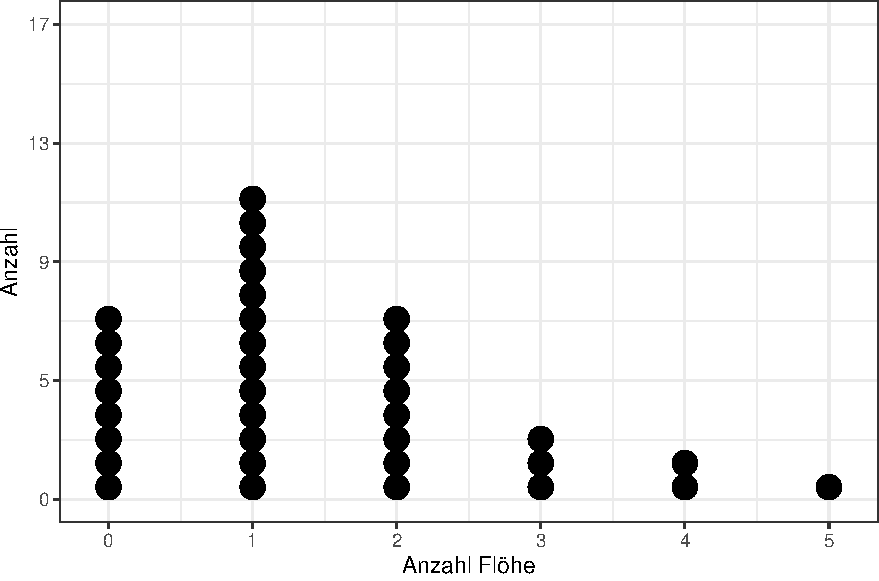
\includegraphics{./eda-ggplot_files/figure-pdf/fig-dotplot-flea-1-1.pdf}

}

\caption{\label{fig-dotplot-flea-1}Die Anzahl von Flöhen auf 39 Hunden.
Jeder Punkt entspricht einem Hund und der entsprechenden Anzahl an
Flöhen auf dem Hund.}

\end{figure}

Wir sehen in Abbildung~\ref{fig-dotplot-flea-1} dasacht Hunde keine
Flöhe hatten - also eine Anzahl an Flöhen von 0. Auf der anderen Seite
hatten zwei Hunde vier Flöhe und ein Hund hatte sogar fünf Flöhe. Wir
sehen also die \emph{Verteilung} der Anzahl an Flöhen über alle unsere
39 Hundebeobachtungen.

Wir schauen uns aber die Verteilung der Anzahl an Flöhen meist nicht in
der Form von gestapelten Punkten an, sondern in der Form eines
Histogramms also einem Balkendiagramm.
Abbildung~\ref{fig-hist-flea-count} zeigt das Histogramm für die Anzahl
der Flöhe.

\begin{Shaded}
\begin{Highlighting}[]
\FunctionTok{ggplot}\NormalTok{(}\AttributeTok{data =}\NormalTok{ dog\_fleas\_hist\_tbl, }\FunctionTok{aes}\NormalTok{(}\AttributeTok{x =}\NormalTok{ flea\_count)) }\SpecialCharTok{+}
  \FunctionTok{geom\_histogram}\NormalTok{(}\AttributeTok{binwidth =} \DecValTok{1}\NormalTok{, }\AttributeTok{fill =} \StringTok{"gray"}\NormalTok{, }\AttributeTok{color =} \StringTok{"black"}\NormalTok{) }\SpecialCharTok{+}
  \FunctionTok{theme\_bw}\NormalTok{() }\SpecialCharTok{+}
  \FunctionTok{labs}\NormalTok{(}\AttributeTok{x =} \StringTok{"Anzahl Flöhe"}\NormalTok{, }\AttributeTok{y =} \StringTok{"Anzahl"}\NormalTok{) }
\end{Highlighting}
\end{Shaded}

\begin{figure}[H]

{\centering 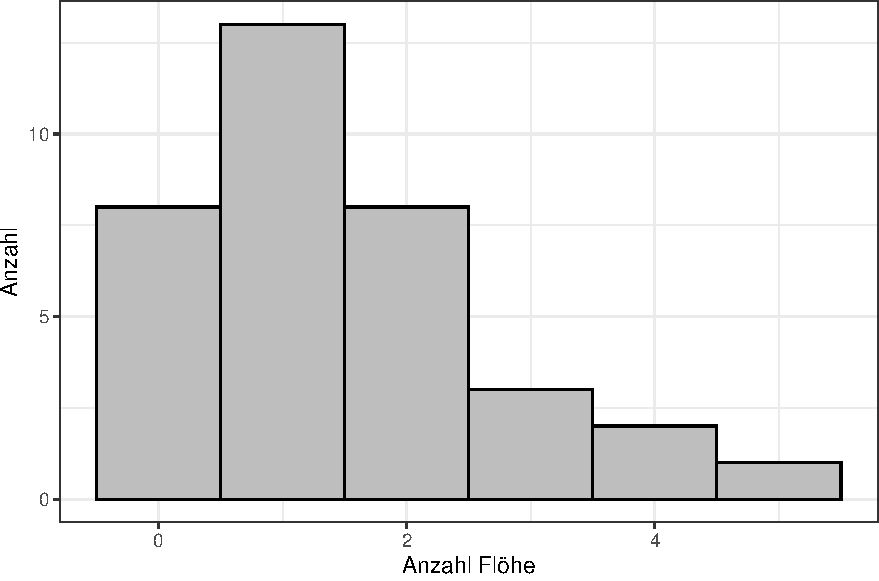
\includegraphics{./eda-ggplot_files/figure-pdf/fig-hist-flea-count-1.pdf}

}

\caption{\label{fig-hist-flea-count}Histogramm der Anzahl von Flöhen auf
39 Hunden.}

\end{figure}

Was sehen wir in der Abbildung~\ref{fig-hist-flea-count}? Anstatt von
gestapelten Punkten sehen wir jetzt Balken, die die jeweilige Anzahl an
Flöhen zusammenfassen. Der Unterschied ist bei einer diskreten Variable
wie der Anzahl (eng. \emph{count}) relativ gering.

Anders sieht es für kontenuierliche Variablen mit Kommazahlen aus.
Schauen wir uns das Gewicht der Flöhe an, so sehen wir, dass es sehr
viele Zahlen gibt, die nur einmal vorkomen.
Abbildung~\ref{fig-hist-flea-1} zeigt das Histogramm für das Geicht der
Flöhe.

\begin{Shaded}
\begin{Highlighting}[]
\FunctionTok{ggplot}\NormalTok{(}\AttributeTok{data =}\NormalTok{ dog\_fleas\_hist\_tbl, }\FunctionTok{aes}\NormalTok{(}\AttributeTok{x =}\NormalTok{ flea\_weight)) }\SpecialCharTok{+}
  \FunctionTok{geom\_histogram}\NormalTok{(}\AttributeTok{binwidth =} \DecValTok{1}\NormalTok{, }\AttributeTok{fill =} \StringTok{"gray"}\NormalTok{, }\AttributeTok{color =} \StringTok{"black"}\NormalTok{) }\SpecialCharTok{+}
  \FunctionTok{theme\_bw}\NormalTok{() }\SpecialCharTok{+}
  \FunctionTok{labs}\NormalTok{(}\AttributeTok{x =} \StringTok{"Gewicht [mg]"}\NormalTok{, }\AttributeTok{y =} \StringTok{"Anzahl"}\NormalTok{) }
\end{Highlighting}
\end{Shaded}

\begin{figure}[H]

{\centering 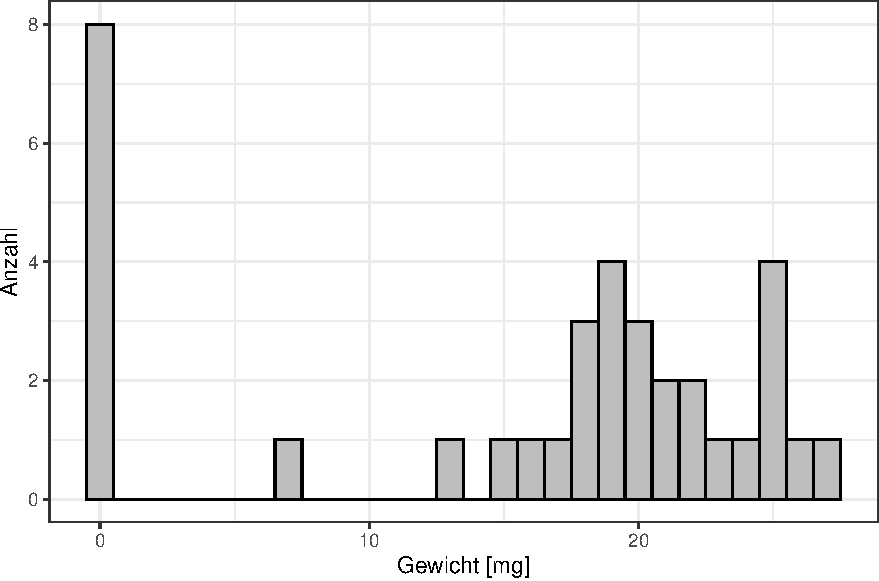
\includegraphics{./eda-ggplot_files/figure-pdf/fig-hist-flea-1-1.pdf}

}

\caption{\label{fig-hist-flea-1}Histogramm des Gewichts von Flöhen auf
39 Hunden.}

\end{figure}

Wie entsteht nun ein Hisotgramm für konetnierliche Zahlen? Schauen wir
uns dafür einmal ein kleineres Datenbeispiel an, in dem wir nur Flöhe
mit einem Gewicht größer als 11 und kleiner als 19 wäheln. Wir nutzen
dazu die Funktion
\texttt{filter(flea\_weight\ \textgreater{}\ 11\ \&\ flea\_weight\ \textless{}\ 19)}.
Wir erhalten folgende Zahlen und das entsprechende Histogramm.

\begin{verbatim}
[1] 13.29 14.91 15.64 16.58 17.66 17.81 18.40 18.64
\end{verbatim}

\begin{figure}

{\centering 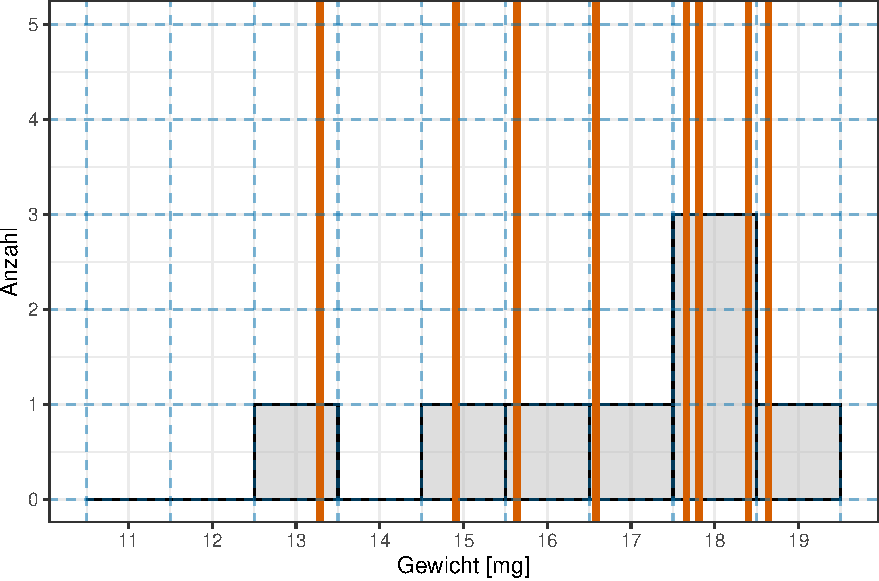
\includegraphics{./eda-ggplot_files/figure-pdf/fig-hist-flea-2-1.pdf}

}

\caption{\label{fig-hist-flea-2}Zusammenhang zwischen den einzelnen
Beobachtungen und der Höhe der einzelnen Balken am Beispiel von acht
Hunden.}

\end{figure}

Abbildung~\ref{fig-hist-flea-2} zeigt das Histogramm der reduzierten
Daten. Die roten vertikalen Linien zeigen die Position der einzelnen
Flohgewichte auf der x-Achse. Die blauen Hilfslinien machen nochmal
klarer, wie hoch die einzelnen Balken sind sowie welche Beobachtungen
auf der x-Achse in den jeweiligen Balken mit eingehen. Wir sehen, dass
wir einen Hund mit Flöhen haben, die zwischen 12.5 und 13.5 wiegen - der
entsprechende Balken erhält die Anzahl von eins. Auf der anderen Seite
sehen wir, dass es drei Hunde mit Flöhen, die zwischen 17.5 und 18.5
wiegen. Daher wächst der Balken auf eine Anzahl von drei.

Wir können mit der Option \texttt{binwidth} in dem
\texttt{geom\_histogram()} einstellen, wie breit auf der x-Achse die
jeweiligen Balken sein sollen. Hier empfiehlt es sich verschiedene
Zahlen für \texttt{binwidth}auszuprobieren.

\hypertarget{density-plot}{%
\subsection{Density Plot}\label{density-plot}}

Eine weitere Möglichkeit sich eine Verteilung anzuschauen, ist die Daten
nicht als Balkendiagramm sondern als Densityplot - also Dichteverteilung
- anzusehen. Im Prinzip verwandeln wir die Balken in eine Kurve. Damit
würden wir im Prinzip unterschiedliche Balkenhöhen ausgleichen udn eine
``glattere'' Darstellung erreichen. Wir wir aber gleich sehen werden,
benötigen wir dazu eine Menge an Beoabchtungen und auch dann ist das
Ergebnis eventuell nicht gut zu interpretieren.

\begin{Shaded}
\begin{Highlighting}[]
\FunctionTok{ggplot}\NormalTok{(}\AttributeTok{data =}\NormalTok{ dog\_fleas\_hist\_tbl, }\FunctionTok{aes}\NormalTok{(}\AttributeTok{x =}\NormalTok{ flea\_count)) }\SpecialCharTok{+}
  \FunctionTok{geom\_histogram}\NormalTok{(}\AttributeTok{binwidth =} \DecValTok{1}\NormalTok{, }\AttributeTok{fill =} \StringTok{"gray"}\NormalTok{, }\AttributeTok{color =} \StringTok{"black"}\NormalTok{) }\SpecialCharTok{+}
  \FunctionTok{theme\_bw}\NormalTok{() }\SpecialCharTok{+}
  \FunctionTok{labs}\NormalTok{(}\AttributeTok{x =} \StringTok{"Anzahl Flöhe"}\NormalTok{, }\AttributeTok{y =} \StringTok{"Anzahl"}\NormalTok{)}

\FunctionTok{ggplot}\NormalTok{(}\AttributeTok{data =}\NormalTok{ dog\_fleas\_hist\_tbl, }\FunctionTok{aes}\NormalTok{(}\AttributeTok{x =}\NormalTok{ flea\_count)) }\SpecialCharTok{+}
  \FunctionTok{geom\_density}\NormalTok{(}\AttributeTok{fill =} \StringTok{"gray"}\NormalTok{, }\AttributeTok{color =} \StringTok{"black"}\NormalTok{) }\SpecialCharTok{+}
  \FunctionTok{theme\_bw}\NormalTok{() }\SpecialCharTok{+}
  \FunctionTok{labs}\NormalTok{(}\AttributeTok{x =} \StringTok{"Anzahl Flöhe"}\NormalTok{, }\AttributeTok{y =} \StringTok{"Häufigkeit"}\NormalTok{) }
\end{Highlighting}
\end{Shaded}

\begin{figure*}

\begin{minipage}[t]{0.50\linewidth}

{\centering 

\raisebox{-\height}{

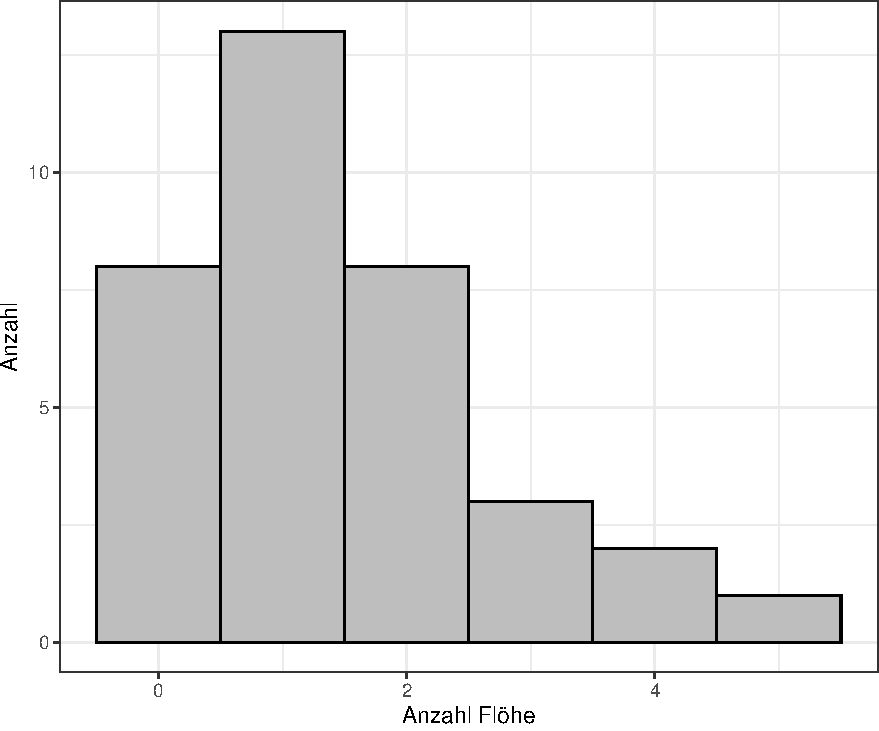
\includegraphics{./eda-ggplot_files/figure-pdf/fig-dens-flea-1-1.pdf}

}

}

\subcaption{\label{fig-dens-flea-1-1}Histogramm}
\end{minipage}%
%
\begin{minipage}[t]{0.50\linewidth}

{\centering 

\raisebox{-\height}{

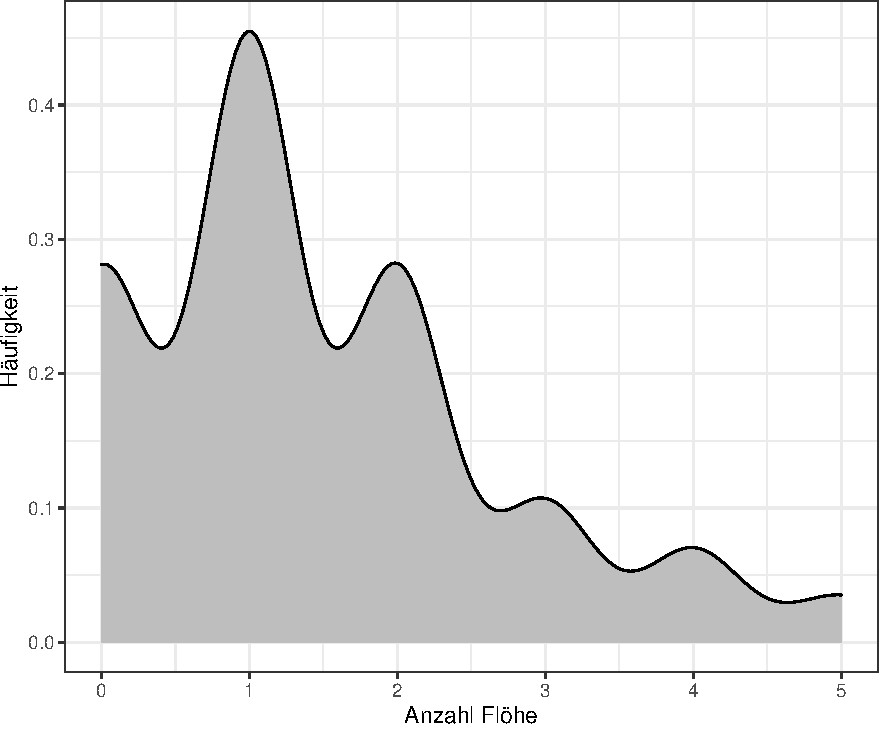
\includegraphics{./eda-ggplot_files/figure-pdf/fig-dens-flea-1-2.pdf}

}

}

\subcaption{\label{fig-dens-flea-1-2}Densityplot}
\end{minipage}%

\caption{\label{fig-dens-flea-1}Zusammenhang von Histogramm und
Densityplot an der Anzahl der Flöhe auf 39 Hunden.}

\end{figure*}

Abbildung~\ref{fig-dens-flea-1} zeigt auf der linken Seite erneut die
Abbildung des Histogramms als Balkendiagramm für die Anzahl der Flöhe
auf den 39 Hunden. Auf der rechten Seite die entsprechenden gleichen
Daten als Denistyplot. Klar ist die Wellenbewegung des Densityplots zu
erkennen. Hier leigen zu wenige Beobachtungen und Kategorien auf der
x-Achse vor, so dass der Densityplot nicht zu empfehlen ist.

\begin{Shaded}
\begin{Highlighting}[]
\FunctionTok{ggplot}\NormalTok{(}\AttributeTok{data =}\NormalTok{ dog\_fleas\_hist\_tbl, }\FunctionTok{aes}\NormalTok{(}\AttributeTok{x =}\NormalTok{ flea\_weight)) }\SpecialCharTok{+}
  \FunctionTok{geom\_histogram}\NormalTok{(}\AttributeTok{binwidth =} \DecValTok{1}\NormalTok{, }\AttributeTok{fill =} \StringTok{"gray"}\NormalTok{, }\AttributeTok{color =} \StringTok{"black"}\NormalTok{) }\SpecialCharTok{+}
  \FunctionTok{theme\_bw}\NormalTok{() }\SpecialCharTok{+}
  \FunctionTok{labs}\NormalTok{(}\AttributeTok{x =} \StringTok{"Gewicht [mg]"}\NormalTok{, }\AttributeTok{y =} \StringTok{"Anzahl"}\NormalTok{) }

\FunctionTok{ggplot}\NormalTok{(}\AttributeTok{data =}\NormalTok{ dog\_fleas\_hist\_tbl, }\FunctionTok{aes}\NormalTok{(}\AttributeTok{x =}\NormalTok{ flea\_weight)) }\SpecialCharTok{+}
  \FunctionTok{geom\_density}\NormalTok{(}\AttributeTok{fill =} \StringTok{"gray"}\NormalTok{, }\AttributeTok{color =} \StringTok{"black"}\NormalTok{) }\SpecialCharTok{+}
  \FunctionTok{theme\_bw}\NormalTok{() }\SpecialCharTok{+}
  \FunctionTok{labs}\NormalTok{(}\AttributeTok{x =} \StringTok{"Gewicht [mg]"}\NormalTok{, }\AttributeTok{y =} \StringTok{"Häufigkeit"}\NormalTok{) }
\end{Highlighting}
\end{Shaded}

\begin{figure*}

\begin{minipage}[t]{0.50\linewidth}

{\centering 

\raisebox{-\height}{

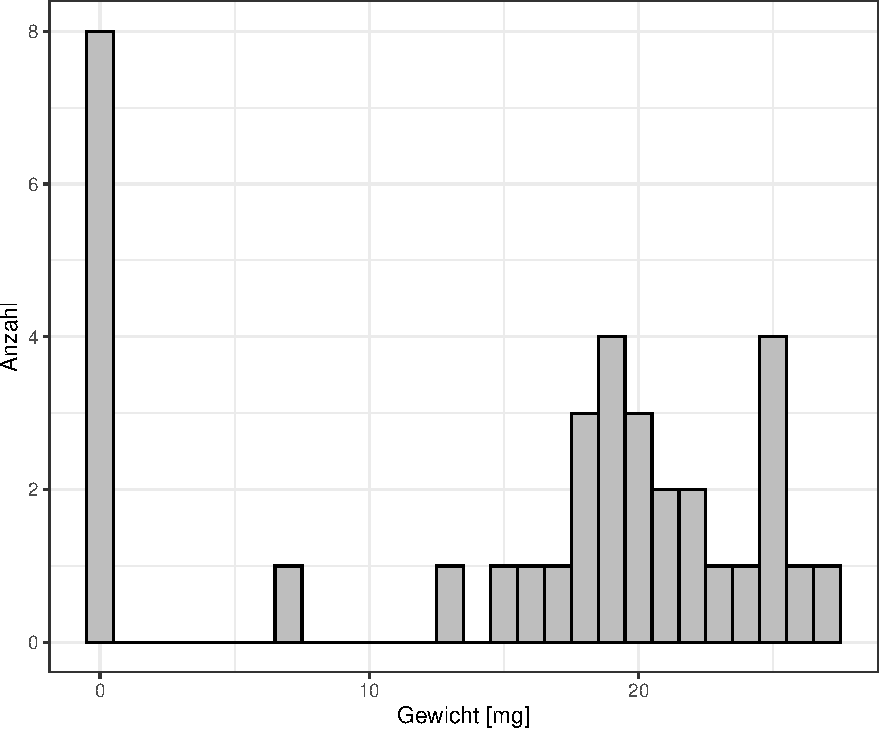
\includegraphics{./eda-ggplot_files/figure-pdf/fig-dens-flea-2-1.pdf}

}

}

\subcaption{\label{fig-dens-flea-2-1}Histogramm}
\end{minipage}%
%
\begin{minipage}[t]{0.50\linewidth}

{\centering 

\raisebox{-\height}{

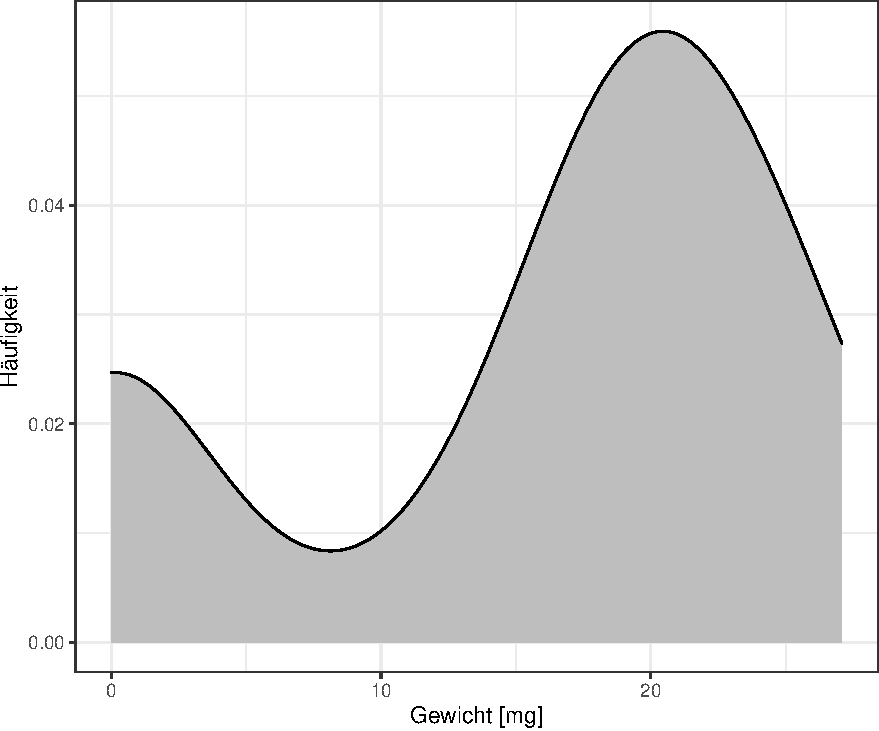
\includegraphics{./eda-ggplot_files/figure-pdf/fig-dens-flea-2-2.pdf}

}

}

\subcaption{\label{fig-dens-flea-2-2}Densityplot}
\end{minipage}%

\caption{\label{fig-dens-flea-2}Zusammenhang von Histogramm und
Densityplot am Gewicht der Flöhe auf 39 Hunden.}

\end{figure*}

Abbildung~\ref{fig-dens-flea-2} zeigt auf der linken Seite erneut die
Abbildung des Histogramms als Balkendiagramm für das Gewicht der Flöhe
auf den 39 Hunden. Insbesondere bei dieser Abbildung erkennst du die
Nachteile des Densityplot. Dadurch das es einen Peak von acht Hunden mit
einem Flohgewicht von 0 gibt, zeigt der Densityplot eine seltsame
Wellenform. Es emppfielt sich daher die Daten zuerst als Histogramm zu
betrachten.

\hypertarget{sec-eda-boxplot}{%
\subsection{Boxplot}\label{sec-eda-boxplot}}

In Kapitel~\ref{sec-desc-stat} haben wir den Median und die Quartile
kennengelernt. Mit dem Boxplot können wir den Median und die Quartile
visualisieren. In Abbildung~\ref{fig-boxplot-drawn} sehen wir einen
Boxplot, der den Median und die Quartile visualisiert. Die Box wird aus
dem IQR gebildet. Der Median wird als Strich in der Box gezeigt. Die
Schnurrhaare (eng. \emph{Whiskers}) sind das 1.5 fache des IQR. Punkte
die außerhalb der Schnurrhaare liegen werden als einzelne Punkte
dargestellt. Diese einzelnen Punkte werden auch als Ausreißer (eng.
\emph{Outlier}) bezeichnet.

\begin{figure*}

{\centering 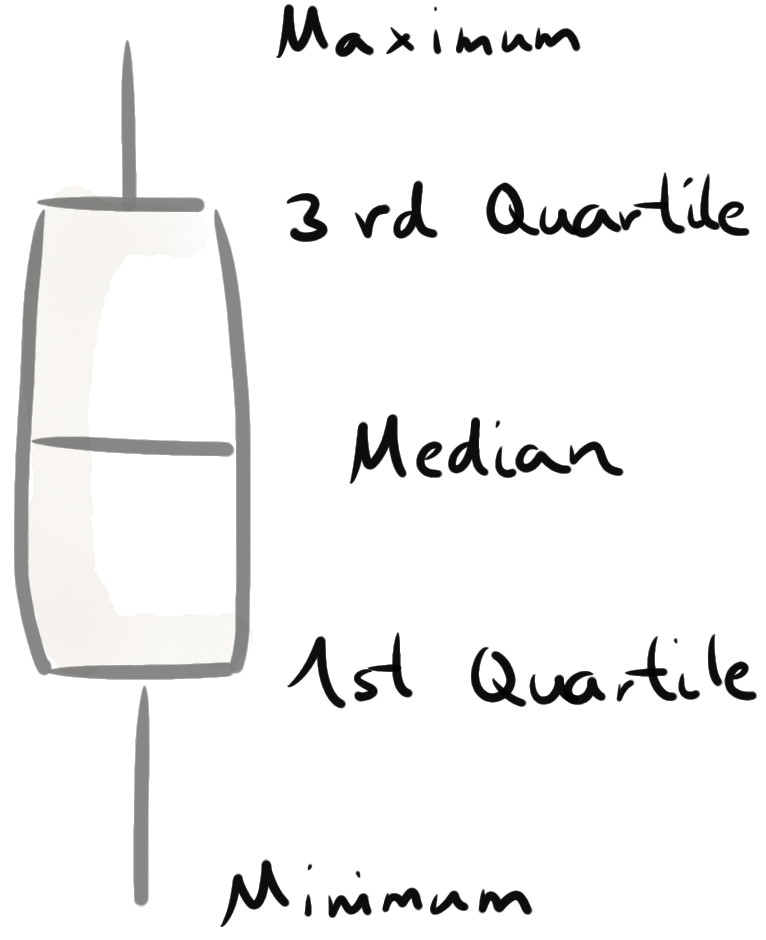
\includegraphics[width=1\textwidth,height=\textheight]{./images/boxplot-drawn.png}

}

\caption{\label{fig-boxplot-drawn}Ein Boxplot der die statistischen
Maßzahlen Median und Quartile visualisiert. Die Box wird aus dem IQR
gebildet. Der Median wird als Strich in der Box gezeigt. Die
Schnurrhaare sind das 1.5 fache des IQR. Punkte die außerhalb der
Schnurrhaare liegen werden als einzele Punkte dargestellt.}

\end{figure*}

In Abbildung~\ref{fig-boxplot-drawn-distribution} sehen wir den
Zusammenhang zwischen einem Histogramm, Densityplot und dem Boxplot. Der
Median \(\tilde{y}\) im Boxplot zeigt die höchste Stelle des
Densityplots an. Durch einen Boxplot kann die Verteilung der
entsprechenden Zahlen abgeschätzt werden.

\begin{figure}

{\centering 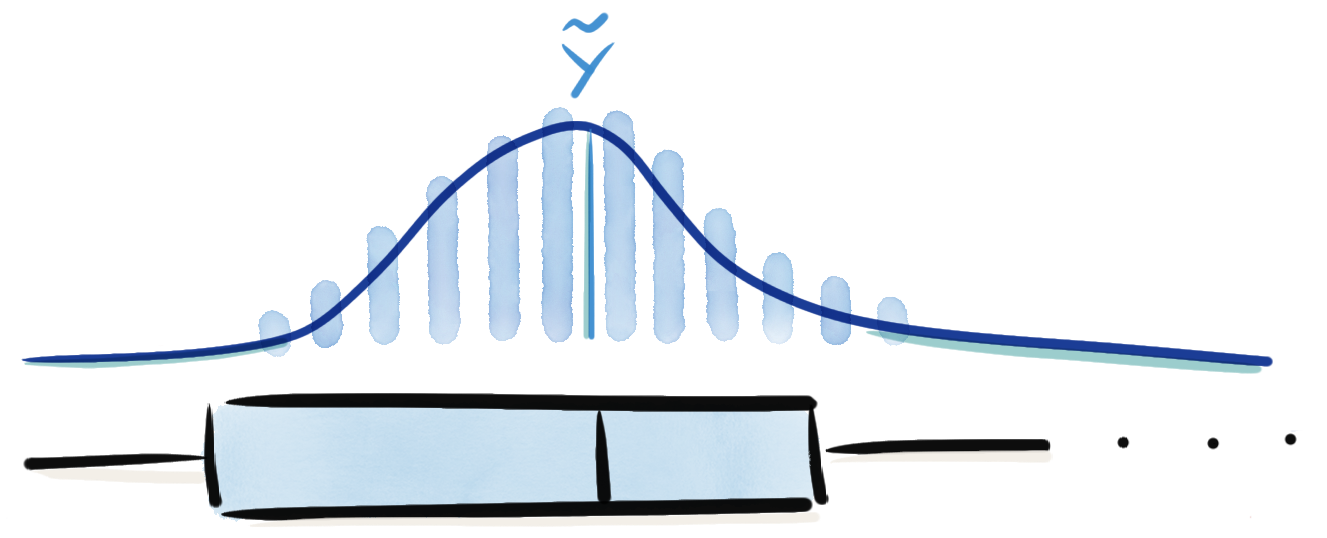
\includegraphics[width=1\textwidth,height=\textheight]{./images/boxplot-drawn-distribution.png}

}

\caption{\label{fig-boxplot-drawn-distribution}Der Zusammenhang von
Histogram, Densityplot und Boxplot.}

\end{figure}

Die ``liegende'' Darstellung des Boxplots dient nur der
Veranschaulichung und dem Verständnis des Zusammenhangs von Histogramm
und Boxplot. In der Abbildung~\ref{fig-boxplot-drawn-flipped} sehen wir
drei Boxplots für einen Faktor mit drei Leveln. Jedes Level wird duch
einen Boxplot dargestellt. Zum Beispiel eine Düngerbehandlung mit drei
Konzentrationen. Auf der x-Achse würden wir die Behandelung finden und
auf der y-Achse das Trockengewicht in {[}kg/ha{]}.

\begin{figure}

{\centering 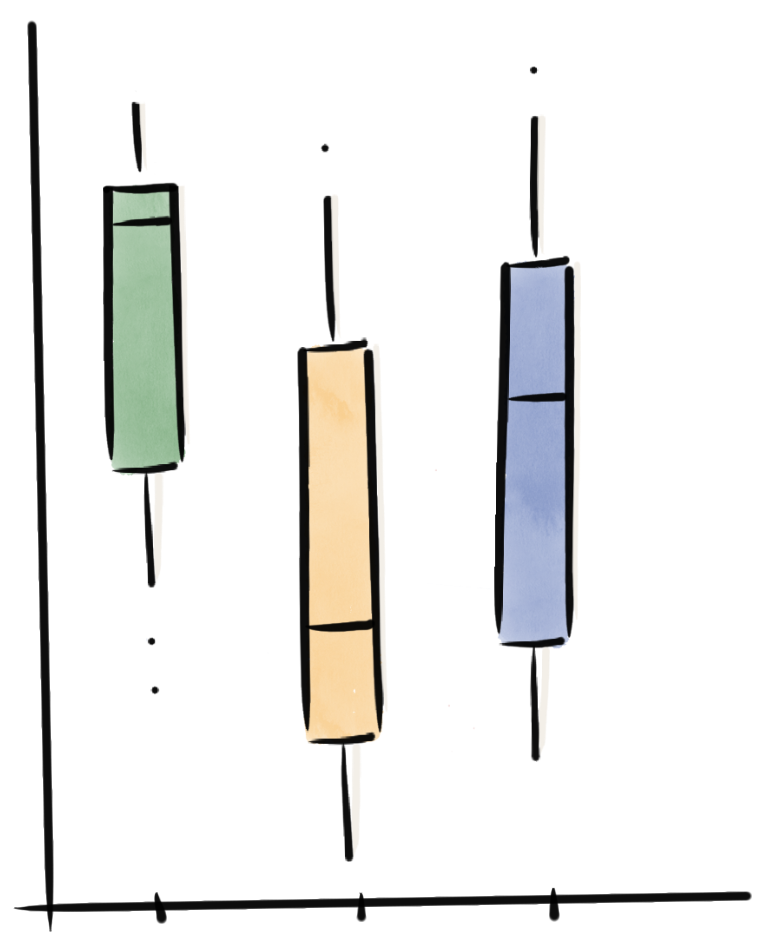
\includegraphics[width=0.6\textwidth,height=\textheight]{./images/boxplot-drawn-flipped.png}

}

\caption{\label{fig-boxplot-drawn-flipped}Typische Darstellung von drei
Gruppen jeweils dargestellt durch einen Boxplot. Boxplots werden in der
Anwendung stehtend dargestellt. Insbesondere wenn die Boxplots mehrere
Gruppen repräsentieren.}

\end{figure}

Wie erstellen wir nun einen Boxplot in R? Zuerst laden wir die Daten mit
der Funktion \texttt{read\_excel()} in R, wenn du die Daten als
\texttt{.xlsx} Datei vorliegen hast. Im XX kannst du nochmal das
Importieren von Daten wiederholen.

\begin{Shaded}
\begin{Highlighting}[]
\NormalTok{flea\_dog\_cat\_tbl }\OtherTok{\textless{}{-}} \FunctionTok{read\_excel}\NormalTok{(}\StringTok{"data/flea\_dog\_cat.xlsx"}\NormalTok{)}
\end{Highlighting}
\end{Shaded}

\begin{figure}

{\centering 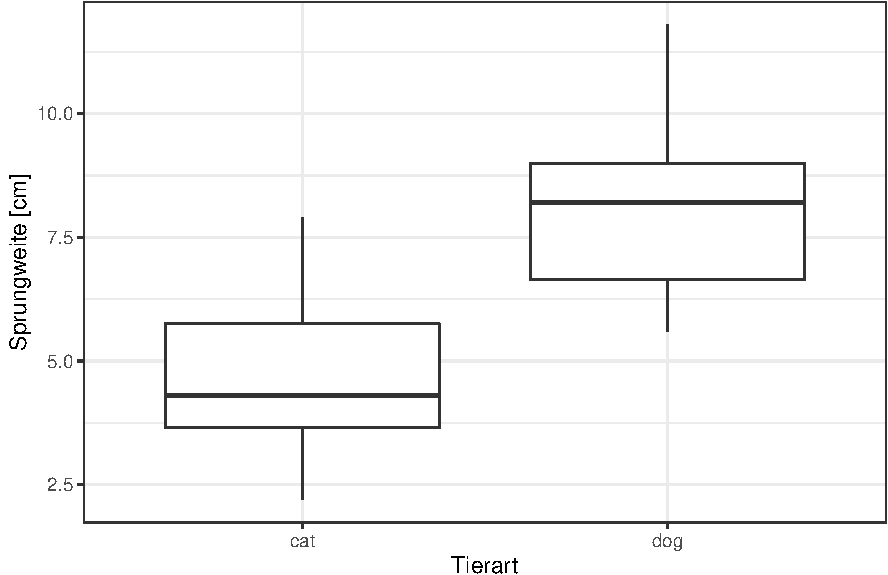
\includegraphics{./eda-ggplot_files/figure-pdf/fig-boxplot-flea-0-1.pdf}

}

\caption{\label{fig-boxplot-flea-0}An 39 Hunden wurde die Anzahl an
Flöhen gezählt.}

\end{figure}

In Abbildung~\ref{fig-boxplot-flea-0} ist der Boxplot für die Daten aus
der Datei \texttt{flea\_dog\_cat.xlsx} dargestellt. Auf der x-Achse
finden wir die Tierart als \texttt{cat} und \texttt{dog}. Auf der
y-Achse ist die Sprungweite in {[}cm{]} dargestellt.

Wir erkennen auf einen Blick, dass die Sprungweite von den Hundeflöhen
weiter ist als die Sprungweite der Katzenflöhe. Im Weiteren können wir
abschätzen, dass die Streuung etwa gleich groß ist. Die Boxen sind in
etwa gleich groß und die Whiskers in etwa gleich lang.

\begin{Shaded}
\begin{Highlighting}[]
\FunctionTok{ggplot}\NormalTok{(}\AttributeTok{data =}\NormalTok{ flea\_dog\_cat\_tbl, }\FunctionTok{aes}\NormalTok{(}\AttributeTok{x =}\NormalTok{ animal, }\AttributeTok{y =}\NormalTok{ jump\_length,}
                                    \AttributeTok{fill =}\NormalTok{ animal)) }\SpecialCharTok{+}
  \FunctionTok{geom\_boxplot}\NormalTok{() }\SpecialCharTok{+}
  \FunctionTok{geom\_jitter}\NormalTok{(}\AttributeTok{width =} \FloatTok{0.25}\NormalTok{, }\AttributeTok{shape =} \DecValTok{1}\NormalTok{) }\SpecialCharTok{+}
  \FunctionTok{theme\_bw}\NormalTok{() }\SpecialCharTok{+}
  \FunctionTok{labs}\NormalTok{(}\AttributeTok{x =} \StringTok{"Tierart"}\NormalTok{, }\AttributeTok{y =} \StringTok{"Sprungweite [cm]"}\NormalTok{) }
\end{Highlighting}
\end{Shaded}

\begin{figure}[H]

{\centering 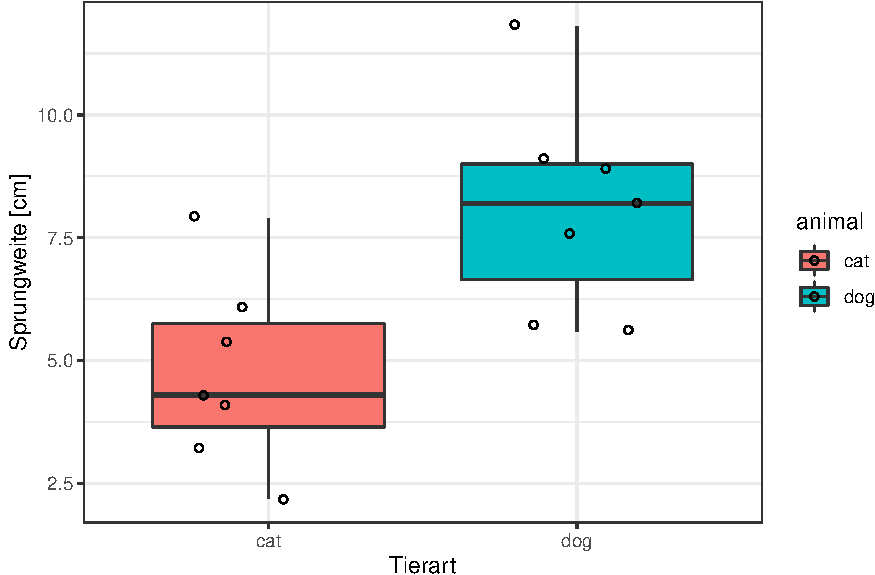
\includegraphics{./eda-ggplot_files/figure-pdf/fig-boxplot-freshmatter-2-1.pdf}

}

\caption{\label{fig-boxplot-freshmatter-2}An 39 Hunden wurde die Anzahl
an Flöhen gezählt.}

\end{figure}

Wir neigen dazu die Boxplots überzuinterpretieren, wenn die Anzahl der
Beobachtungen klein ist. Deshalb können wir mit dem
\texttt{geom\_jitter()} noch die Beobachtungen zu den Boxplot ergänzen,
dargestellt in Abbildung~\ref{fig-boxplot-freshmatter-2}. Die Funktion
\texttt{geom\_jitter()} streut die Punkte zufällig, so dass keine Punkte
übereinanderliegen. Wir haben hier die Streuuweite durch die Option
\texttt{width\ =\ 0.25} etwas eingeschränkt. Darüber hinaus habe wir das
Aussehen der Punkte mit \texttt{shape\ =\ 1} geändert, so dass wir die
Jitter-Punkte von den potenziellen Ausreißer-Punkten unterscheiden
können. Du kannst auch andere Zahlen hinter \texttt{shape} eintragen um
verschiedene Punktesymbole durchzuprobieren. Eine Übersicht an
\texttt{shapes} findest du auch hier unter
\href{http://www.cookbook-r.com/Graphs/Shapes_and_line_types/}{Cookbook
for R \textgreater{} Graphs \textgreater{} Shapes and line types}.

\hypertarget{sec-eda-dotplot}{%
\subsection{Dotplot}\label{sec-eda-dotplot}}

Wenn wir weniger als fünf Beobachtungen haben, dann ist meist ein
Boxplot verzerrend. Wir sehen eine Box und glauben, dass wir viele
Datenpunkte vorliegen haben. Bei 3 bis 7 Beobachtungen je Gruppe bietet
sich der Dotplot als eine Lösung an. Wir stellen hier alle Beobachtungen
als einzelne Punkte dar.

Wie erstellen wir nun einen Dotplot in R? Zuerst laden wir die Daten mit
der Funktion \texttt{read\_excel()} in R, wenn du die Daten als
\texttt{.xlsx} Datei vorliegen hast. Im XX kannst du nochmal das
Importieren von Daten wiederholen.

\begin{Shaded}
\begin{Highlighting}[]
\NormalTok{flea\_dog\_cat\_tbl }\OtherTok{\textless{}{-}} \FunctionTok{read\_excel}\NormalTok{(}\StringTok{"data/flea\_dog\_cat.xlsx"}\NormalTok{)}
\end{Highlighting}
\end{Shaded}

\begin{Shaded}
\begin{Highlighting}[]
\FunctionTok{ggplot}\NormalTok{(}\AttributeTok{data =}\NormalTok{ flea\_dog\_cat\_tbl, }\FunctionTok{aes}\NormalTok{(}\AttributeTok{x =}\NormalTok{ animal, }\AttributeTok{y =}\NormalTok{ grade,}
                                    \AttributeTok{fill =}\NormalTok{ animal)) }\SpecialCharTok{+}
  \FunctionTok{geom\_dotplot}\NormalTok{(}\AttributeTok{binaxis =} \StringTok{"y"}\NormalTok{, }\AttributeTok{stackdir =} \StringTok{"center"}\NormalTok{) }\SpecialCharTok{+}
  \FunctionTok{theme\_bw}\NormalTok{() }\SpecialCharTok{+}
  \FunctionTok{labs}\NormalTok{(}\AttributeTok{x =} \StringTok{"Tierart"}\NormalTok{, }\AttributeTok{y =} \StringTok{"Boniturnote [1{-}9]"}\NormalTok{) }
\end{Highlighting}
\end{Shaded}

\begin{figure}[H]

{\centering 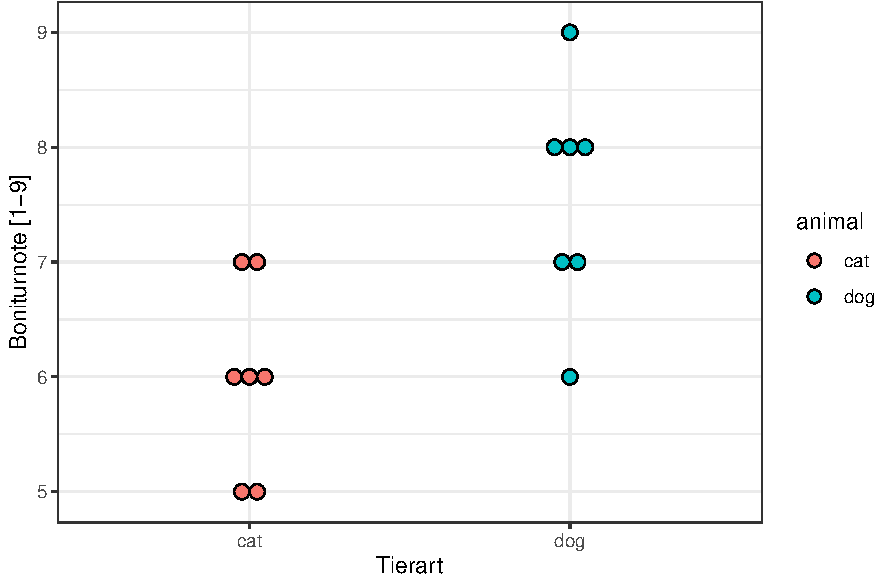
\includegraphics{./eda-ggplot_files/figure-pdf/fig-dotplot-flea-eda-0-1.pdf}

}

\caption{\label{fig-dotplot-flea-eda-0}Der Dotplot für die Anzahl der
Flöhe für die beiden Tierarten Hund und Katze.}

\end{figure}

In Abbildung~\ref{fig-dotplot-flea-eda-0} sehen wir den Dotplot aus der
Datei \texttt{flea\_dog\_cat.xlsx}. Auf der x-Achse sind die Level des
Faktors \texttt{animal} dargestellt und auf der y-Achse die
Notenbewertung \texttt{grade} der einzelnen Hunde und Katzen. Die
Funktion \texttt{geom\_dotplot()} erschafft das Layer für die Dots bzw.
Punkte. Wir müssen in der Funktion noch zwei Dinge angeben, damit der
Plot so aussieht, dass wir den Dotplot gut interpretieren können. Zum
einen müssen wir die Option \texttt{binaxis\ =\ y} wählen, damit die
Punkte horizontal geordent werden. Zum anderen wollen wir auch, dass die
Punkte zentriert sind und nutzen dafür die Option
\texttt{stackdir\ =\ center}.

\begin{Shaded}
\begin{Highlighting}[]
\FunctionTok{ggplot}\NormalTok{(}\AttributeTok{data =}\NormalTok{ flea\_dog\_cat\_tbl, }\FunctionTok{aes}\NormalTok{(}\AttributeTok{x =}\NormalTok{ animal, }\AttributeTok{y =}\NormalTok{ grade,}
                            \AttributeTok{fill =}\NormalTok{ animal)) }\SpecialCharTok{+}
  \FunctionTok{geom\_dotplot}\NormalTok{(}\AttributeTok{binaxis =} \StringTok{"y"}\NormalTok{, }\AttributeTok{stackdir =} \StringTok{"center"}\NormalTok{) }\SpecialCharTok{+}
  \FunctionTok{stat\_summary}\NormalTok{(}\AttributeTok{fun =}\NormalTok{ median, }\AttributeTok{fun.min =}\NormalTok{ median, }\AttributeTok{fun.max =}\NormalTok{ median,}
               \AttributeTok{geom =} \StringTok{"crossbar"}\NormalTok{, }\AttributeTok{width =} \FloatTok{0.5}\NormalTok{) }\SpecialCharTok{+}
  \FunctionTok{theme\_bw}\NormalTok{() }\SpecialCharTok{+}
  \FunctionTok{labs}\NormalTok{(}\AttributeTok{x =} \StringTok{"Tierart"}\NormalTok{, }\AttributeTok{y =} \StringTok{"Boniturnote [1{-}9]"}\NormalTok{) }
\end{Highlighting}
\end{Shaded}

\begin{figure}[H]

{\centering 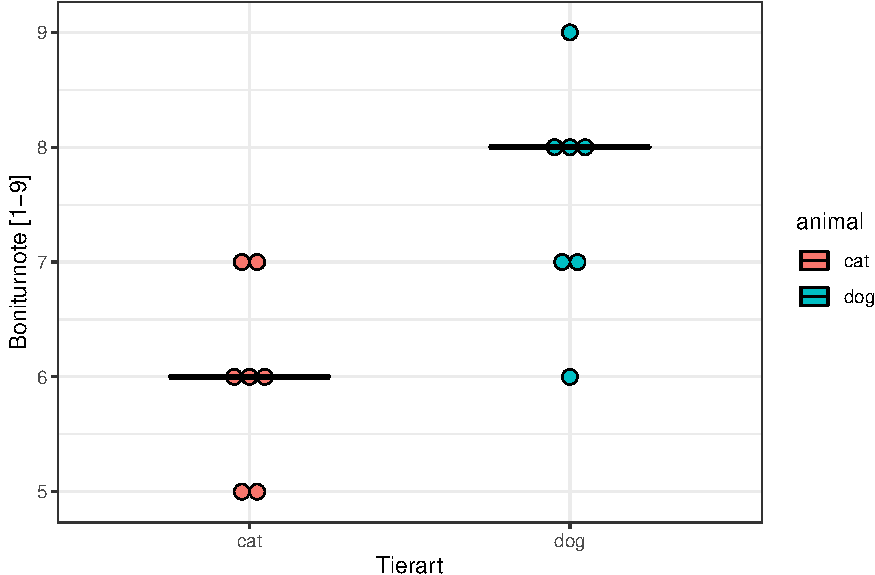
\includegraphics{./eda-ggplot_files/figure-pdf/fig-dotplot-flea-eda-1-1.pdf}

}

\caption{\label{fig-dotplot-flea-eda-1}Der Dotplot für die Anzahl der
Flöhe für die beiden Tierarten Hund und Katze. Die schwarze Linie stelt
den Median für die beiden Tierarten dar.}

\end{figure}

Nun macht es wenig Sinn bei sehr wenigen Beobachtungen noch statistische
Maßzahlen mit in den Plot zu zeichnen. Sonst hätten wir auch gleich
einen Boxplot als Visualisierung der Daten wählen können. In
Abbildung~\ref{fig-dotplot-flea-eda-1} sehen wir die Ergänzung des
Medians. Hier müssen wir etwas mehr angeben, aber immerhin haben wir so
eine Idee, wo die ``meisten'' Beobachtungen wären. Aber auch hier ist
Vorsicht geboten. Wir haben sehr wenige Beobachtungen, so dass eine
Beobachtung mehr oder weniger große Auswirkungen auf den Median und die
Interpretation hat.

\hypertarget{sec-eda-scatter}{%
\subsection{Scatterplot}\label{sec-eda-scatter}}

Der Scatterplot wird auch xy-Plot genannt. Wir stellen in einem
Scatterplot zwei kontenuierliche Variablen dar. Dann wollen wir eine
Linie durch die Punkte legen. Im Prinzip fragen wir uns, wie hänge die
Werte auf der y-Achse von den Werten auf der x-Achse ab? Wenn sich also
die Werte auf der x-Achse erhöhen, wie verhalten sich dann die Werte auf
der y-Achse?

\begin{Shaded}
\begin{Highlighting}[]
\FunctionTok{ggplot}\NormalTok{(}\AttributeTok{data =}\NormalTok{ flea\_dog\_cat\_tbl, }\FunctionTok{aes}\NormalTok{(}\AttributeTok{x =}\NormalTok{ flea\_count, }\AttributeTok{y =}\NormalTok{ jump\_length)) }\SpecialCharTok{+}
  \FunctionTok{geom\_point}\NormalTok{() }\SpecialCharTok{+}
  \FunctionTok{stat\_smooth}\NormalTok{(}\AttributeTok{method =} \StringTok{"lm"}\NormalTok{, }\AttributeTok{se =} \ConstantTok{FALSE}\NormalTok{) }\SpecialCharTok{+}
  \FunctionTok{theme\_bw}\NormalTok{() }\SpecialCharTok{+}
  \FunctionTok{labs}\NormalTok{(}\AttributeTok{x =} \StringTok{"Anzahl der Flöhe"}\NormalTok{, }\AttributeTok{y =} \StringTok{"Sprungweite in [cm]"}\NormalTok{) }
\end{Highlighting}
\end{Shaded}

\begin{figure}[H]

{\centering 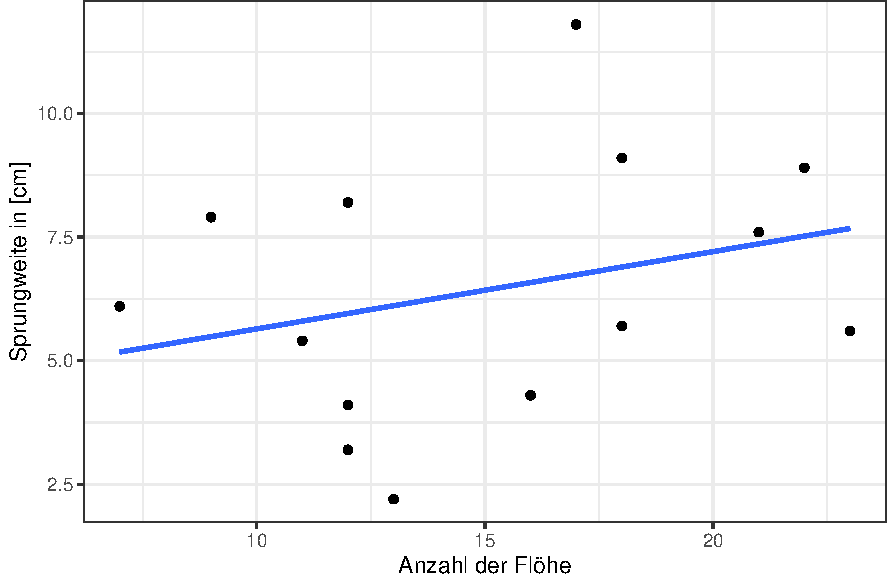
\includegraphics{./eda-ggplot_files/figure-pdf/fig-scatter-flea-0-1.pdf}

}

\caption{\label{fig-scatter-flea-0}Zusammenhang zwischen der Sprungweite
in {[}cm{]} und der Anzahl an Flöhen auf den 39 Hunden. Jeder Punkt
stellt einen Hund dar.}

\end{figure}

Abbildung~\ref{fig-scatter-flea-0} zeigt den Scatterplot für die Spalte
\texttt{flea\_count} auf der x-Achse und \texttt{jump\_length} auf der
y-Achse. Mit der Funktion \texttt{geom\_point()} können wir die
Punktepaare für jede Beobachtung zeichnen. In unserem Fall zeichnen wir
mit der Funktion \texttt{stat\_smooth()} noch die entsprechende Grade
durch die Punkte. Es handelt sich hierbei um eine Regression. Du kannst
im Kapitel XX mehr darüber erfahren.

\hypertarget{sec-eda-mosaic}{%
\subsection{Mosaic Plot}\label{sec-eda-mosaic}}

Wenn wir zwei Spalten visualisieren wollen, die aus zwei Faktoren
bestehen mit jeweils zwei Leveln, dann nutzen wir den Mosaic Plot. Wir
nutzen den Datensatz \texttt{flea\_dog\_cat.xlsx} mit vierzehn
Beobachtungen. Schauen wir uns einmal die 2x2 Kreuztabelle der beiden
Spalten \texttt{animal} and \texttt{infected} an.

\begin{Shaded}
\begin{Highlighting}[]
\NormalTok{flea\_dog\_cat\_tbl }\SpecialCharTok{\%\textgreater{}\%}
  \FunctionTok{mutate}\NormalTok{(}\AttributeTok{animal =} \FunctionTok{factor}\NormalTok{(animal, }\AttributeTok{levels =} \FunctionTok{c}\NormalTok{(}\StringTok{"dog"}\NormalTok{, }\StringTok{"cat"}\NormalTok{))) }\SpecialCharTok{\%\textgreater{}\%} 
  \FunctionTok{tabyl}\NormalTok{(animal, infected) }
\end{Highlighting}
\end{Shaded}

\begin{verbatim}
 animal 0 1
    dog 4 3
    cat 5 2
\end{verbatim}

Wir sehen in der Tabelle, dass wir mehr uninfizierte Tiere (n = 9) als
infizierte Tiere haben (n = 5). Die Aufteilung zwischen den beiden
Tierarten ist nahezu gleich. Im folgenden wollen wir diese Tabelle durch
einen Mosaic Plot einmal visualisieren.

\begin{Shaded}
\begin{Highlighting}[]
\FunctionTok{ggplot}\NormalTok{(}\AttributeTok{data =}\NormalTok{ flea\_dog\_cat\_tbl) }\SpecialCharTok{+}
  \FunctionTok{geom\_mosaic}\NormalTok{(}\FunctionTok{aes}\NormalTok{(}\AttributeTok{x =} \FunctionTok{product}\NormalTok{(animal, infected), }\AttributeTok{fill =}\NormalTok{ animal)) }
\end{Highlighting}
\end{Shaded}

\begin{figure}[H]

{\centering 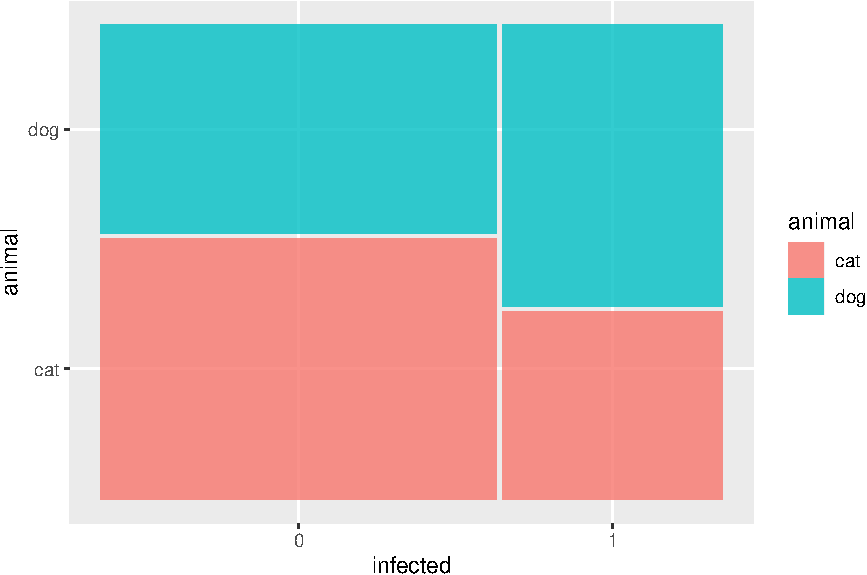
\includegraphics{./eda-ggplot_files/figure-pdf/fig-mosaic-flea-0-1.pdf}

}

\caption{\label{fig-mosaic-flea-0}Visualisierung einer 2x2 Tabelle als
Mosaic Plot. Die unterschiedlich großen Flächen geben die Verhältnisse
wieder.}

\end{figure}

Abbildung~\ref{fig-mosaic-flea-0} zeigt den Mosaic Plot für die Variable
\texttt{animal} and \texttt{infected}. Die untrschiedlich großen Flächen
bilden die Verhältnisse der 2x2 Tabelle ab. So sehen wir, dass es mehr
uninfizierte Tiere als infizierte Tiere gibt. Am meisten gibt es
uninfizierte Katzen. Am wenigstens treten infizierte Katzen auf.

\hypertarget{uxfcberschriften-achsen-und-legenden}{%
\subsection{Überschriften, Achsen und
Legenden}\label{uxfcberschriften-achsen-und-legenden}}

Wenn du mehr machen willst, also die Überschriften anpassen oder aber
die Achsenbeschriftung ändern, dann gibt es hier global Hilfe im
\href{https://ggplot2.tidyverse.org/reference/index.html}{ggplot
Manual}. Die Webseite
\href{https://ggplot2.tidyverse.org/reference/index.html}{R Cookbook}
hat auch spezielle Hilfe für ggplot().

\begin{itemize}
\tightlist
\item
  \href{http://www.cookbook-r.com/Graphs/Titles_(ggplot2)/}{Überschriften
  von Abbildungen}
\item
  \href{http://www.cookbook-r.com/Graphs/Axes_(ggplot2)/}{Achsenbeschriftung}
\item
  \href{http://www.cookbook-r.com/Graphs/Legends_(ggplot2)/}{Legende}
\item
  \href{http://www.cookbook-r.com/Graphs/Colors_(ggplot2)/}{Farben}
\end{itemize}

{\marginnote{\begin{footnotesize}Im Kapitel~\ref{sec-r-tutorium} findest
du Informationen zum R Tutorium, wann und wo es
stattfindet.\end{footnotesize}}}

In Abbildung~\ref{fig-labels-0} siehst du eine Abbildung mit Titel und
veränderten Beschriftungen. Die Möglichkeiten sind nahezu unbegrenzt und
sprengen auch hier den Rahmen. Im Zweifel im R Tutorium vorbeischauen
oder aber in der Vorlesung fragen.

\begin{Shaded}
\begin{Highlighting}[]
\FunctionTok{ggplot}\NormalTok{(}\AttributeTok{data =}\NormalTok{ flea\_dog\_cat\_tbl, }\FunctionTok{aes}\NormalTok{(}\AttributeTok{x =}\NormalTok{ animal, }\AttributeTok{y =}\NormalTok{ jump\_length,}
                                    \AttributeTok{fill =}\NormalTok{ animal)) }\SpecialCharTok{+}
  \FunctionTok{geom\_boxplot}\NormalTok{() }\SpecialCharTok{+}
  \FunctionTok{labs}\NormalTok{(}\AttributeTok{title =} \StringTok{"Frischgewicht in Abhängigkeit von der Behandlung"}\NormalTok{,}
       \AttributeTok{x =} \StringTok{"Behandlung"}\NormalTok{, }\AttributeTok{y =} \StringTok{"Frischgewicht in kg/ha"}\NormalTok{) }\SpecialCharTok{+}
  \FunctionTok{scale\_x\_discrete}\NormalTok{(}\AttributeTok{labels =} \FunctionTok{c}\NormalTok{(}\StringTok{"Katze"}\NormalTok{, }\StringTok{"Hund"}\NormalTok{)) }\SpecialCharTok{+}
  \FunctionTok{scale\_fill\_discrete}\NormalTok{(}\AttributeTok{name =} \StringTok{"Behandlung"}\NormalTok{, }\AttributeTok{labels =} \FunctionTok{c}\NormalTok{(}\StringTok{"Katze"}\NormalTok{, }\StringTok{"Hund"}\NormalTok{)) }\SpecialCharTok{+}
  \FunctionTok{theme\_bw}\NormalTok{() }
\end{Highlighting}
\end{Shaded}

\begin{figure}[H]

{\centering 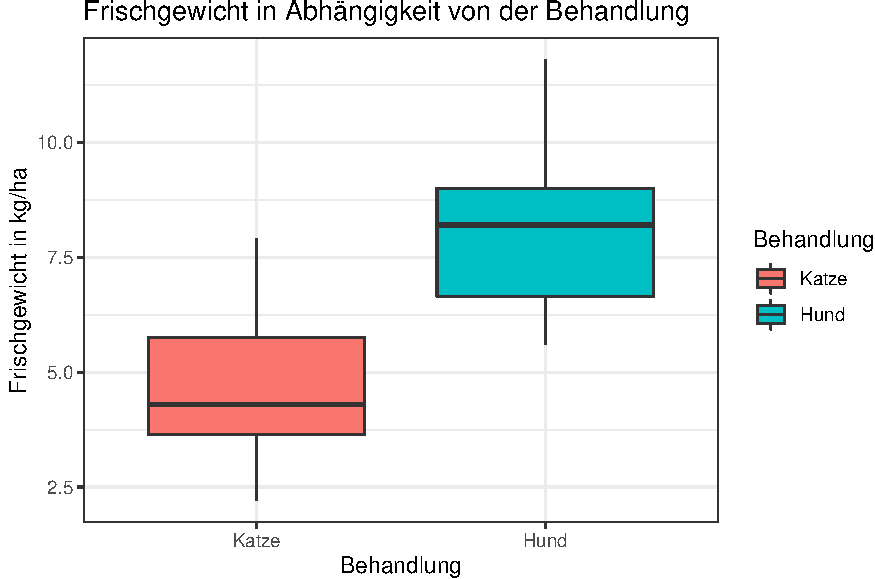
\includegraphics{./eda-ggplot_files/figure-pdf/fig-labels-0-1.pdf}

}

\caption{\label{fig-labels-0}Beispielhafte Abbildung mit Titel und
geänderter Achsenbeschrittung}

\end{figure}

\hypertarget{die-okabe-ito-farbpalette}{%
\subsection{Die Okabe-Ito Farbpalette}\label{die-okabe-ito-farbpalette}}

\marginnote{\begin{footnotesize}

Mehr zum R Paket \texttt{see} auf der
\href{https://easystats.github.io/see/index.html}{Hilfeseite des
Paketes}

\end{footnotesize}}

Neben den klassischen Farben im R Paket \texttt{ggplot}gibt es noch
weit, weit mehr Farbpaletten. Wir nutzen in der Folge immer wieder die
Okabe-Ito Farbpalette aus dem R Paket \texttt{see}. Die Okabe-Ito
Farbpalette ist speziell so gebaut, dass die Farben sich gut für
farbenblinde Personen unterscheiden. Der Kontrast zwischen den Farben
ist sehr gut. Wenn du eine andere Farbpalette nutzen willst, findest du
hier noch andere
\href{https://easystats.github.io/see/articles/seecolorscales.html}{Color
Scales}.

\begin{Shaded}
\begin{Highlighting}[]
\FunctionTok{ggplot}\NormalTok{(}\AttributeTok{data =}\NormalTok{ flea\_dog\_cat\_tbl, }
       \FunctionTok{aes}\NormalTok{(}\AttributeTok{x =}\NormalTok{ animal, }\AttributeTok{y =}\NormalTok{ jump\_length,}
           \AttributeTok{fill =}\NormalTok{ animal)) }\SpecialCharTok{+}
  \FunctionTok{geom\_boxplot}\NormalTok{() }\SpecialCharTok{+}
  \FunctionTok{scale\_fill\_okabeito}\NormalTok{() }\SpecialCharTok{+}
  \FunctionTok{theme\_bw}\NormalTok{()}
\end{Highlighting}
\end{Shaded}

\begin{figure}[H]

{\centering 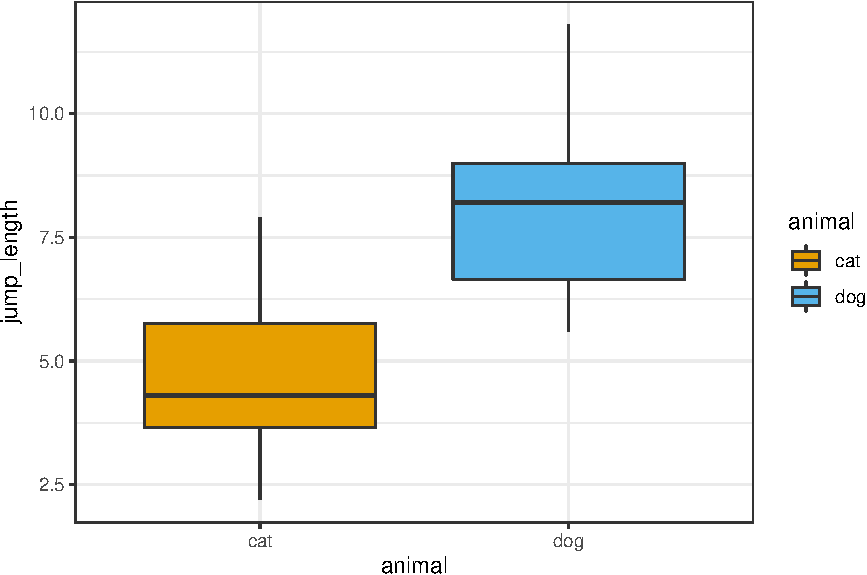
\includegraphics{./eda-ggplot_files/figure-pdf/fig-labels-see-0-1.pdf}

}

\caption{\label{fig-labels-see-0}Beispielhafte Abbildung der Okabe-Ito
Farbpalette für Boxplots.}

\end{figure}

\begin{Shaded}
\begin{Highlighting}[]
\FunctionTok{ggplot}\NormalTok{(}\AttributeTok{data =}\NormalTok{ flea\_dog\_cat\_tbl, }
       \FunctionTok{aes}\NormalTok{(}\AttributeTok{x =}\NormalTok{ animal, }\AttributeTok{y =}\NormalTok{ jump\_length,}
           \AttributeTok{color =}\NormalTok{ animal)) }\SpecialCharTok{+}
  \FunctionTok{geom\_point}\NormalTok{() }\SpecialCharTok{+}
  \FunctionTok{scale\_color\_okabeito}\NormalTok{() }\SpecialCharTok{+}
  \FunctionTok{theme\_bw}\NormalTok{()}
\end{Highlighting}
\end{Shaded}

\begin{figure}[H]

{\centering 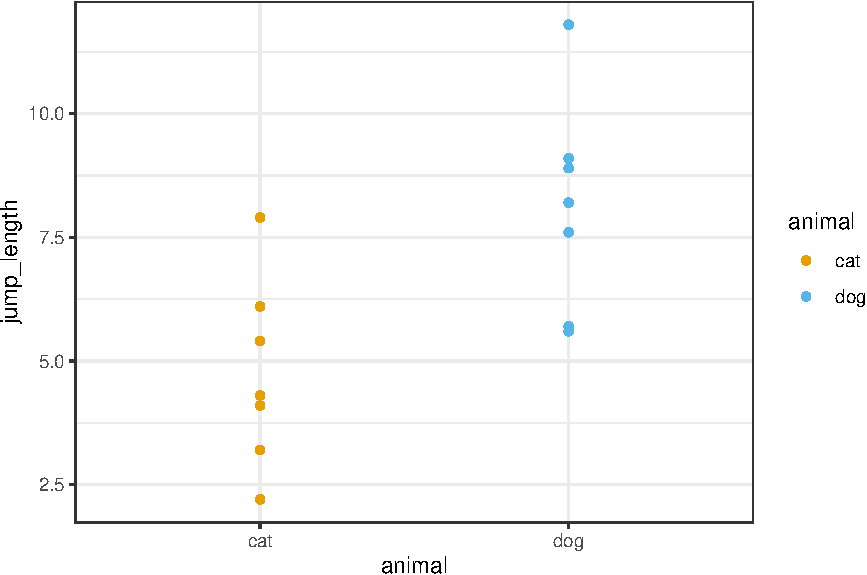
\includegraphics{./eda-ggplot_files/figure-pdf/fig-labels-see-1-1.pdf}

}

\caption{\label{fig-labels-see-1}Beispielhafte Abbildung der Okabe-Ito
Farbpalette für Scatterplots.}

\end{figure}

\part{Frequentistische Hypothesentests}

\begin{tcolorbox}[enhanced jigsaw, bottomrule=.15mm, toptitle=1mm, colbacktitle=quarto-callout-tip-color!10!white, opacityback=0, bottomtitle=1mm, leftrule=.75mm, toprule=.15mm, breakable, rightrule=.15mm, title=\textcolor{quarto-callout-tip-color}{\faLightbulb}\hspace{0.5em}{Grundlagen der Wissenschaft und Falsifikationsprinzip}, coltitle=black, colframe=quarto-callout-tip-color-frame, colback=white, titlerule=0mm, left=2mm, arc=.35mm, opacitybacktitle=0.6]
Du findest auf YouTube \href{https://youtu.be/h45ftLNsspM}{Grundlagen
der Wissenschaft und Falsifikationsprinzip} als Video.
\end{tcolorbox}

Das statistische Testen - eine Geschichte voller Missverständnisse. Wir
wollen uns in diesem Kapitel mit den Grundlagen des frequentistischen
Hypothesentestens beschäftigen. Wenn ich hier einen Unterschied mache,
dann muss es ja auch noch ein anderes Hypothesentesten geben. Ja, das
nennt man dann bayesianische Statistik und kommt eventuell mal später.
Wir konzentrieren uns aber zuerst auf frequentistische Hypothesentesten
was seit gut hundert Jahren genutzt wird. Ich werde hier textlich nur
einen kurzen Einstieg liefern. Vielleicht wird es in den folgenden
Jahren länger aber aktuell (Ende 2022) bleiben wir hier bei einem kurzen
Einstieg.

{\marginnote{\begin{footnotesize}Forschung basiert auf dem
Falsifikationsprinzip. Wir können \textbf{nur ablehnen} und behalten das
weniger schlechte Modell bei.\end{footnotesize}}}

Beginnen wir mit der Logik der Forschung oder allgemeiner formuliert,
als die Grundlage der Wissenschaft. Wir basieren all unsere
Entscheidungen in der Wissenschaft auf dem Falsifikationsprinzip. Also
bitte merken, wir können nur ablehnen (eng. \emph{reject}).

\begin{tcolorbox}[enhanced jigsaw, bottomrule=.15mm, toptitle=1mm, colbacktitle=quarto-callout-note-color!10!white, opacityback=0, bottomtitle=1mm, leftrule=.75mm, toprule=.15mm, breakable, rightrule=.15mm, title=\textcolor{quarto-callout-note-color}{\faInfo}\hspace{0.5em}{Logik der Forschung}, coltitle=black, colframe=quarto-callout-note-color-frame, colback=white, titlerule=0mm, left=2mm, arc=.35mm, opacitybacktitle=0.6]
„Das ist die Logik der Forschung, die nie verifizieren, sondern immer
nur jene Erklärungen beibehalten kann, die beim derzeitigen
Erkenntnisstand am wenigsten falsifiziert sind.'' -- Wößmann, L.

Wir ersetzen schlechte Modelle (der Wirklichkeit) durch weniger
schlechte Modelle (der Wirklichkeit).
\end{tcolorbox}

Wir wollen hier auf keinen Fall die Leistungen von Altvorderen
schmälern. Dennoch hatten
\href{https://en.wikipedia.org/wiki/Ronald_Fisher}{Ronald Fischer (1890
- 1962)}, als der Begründer der Statistik, andere Vorraussetzungen als
wir heutzutage. Als wichtigster Unterschied sei natürlich das Gerät
genannt, an dem du gerade diese Zeilen liest: dem Computer. Selbst die
Erstellung einfachster Abbildungen war sehr, sehr zeitaufwendig. Die
Berechnung von Zahlen lohnte sich mehr, als die Zahlen zu visualisieren.
Insbesondere wenn wir die Explorative Datenanalyse nach
\href{https://en.wikipedia.org/wiki/John_Tukey}{John Tukey (1915 -
2000)} durchführen. Undenkbar zu den Zeiten von Ronald Fischer mehrere
Abbildungen unterschiedlich nach Faktoren einzufärben und sich die Daten
\emph{anzugucken}.

{\marginnote{\begin{footnotesize}Über die Nullhypothese erfährst du mehr
in dem folgenden \textbf{?@sec-hypothesen}\end{footnotesize}}}

Neben dieser Begrenzung von moderner Rechenkapazität um 1900 gab es noch
eine andere ungünstige Entwicklung. Stark vereinfacht formuliert
entwickelte Ronald Fischer statistische Werkzeuge um abzuschätzen wir
wahrscheinlich die Nullhypothese unter dem Auftreten der beobachteten
Daten ist. Nun ist es aber so, dass wir ja auch eine Entscheidung
treffen wollen. Nach der Logik der Forschung wollen wir ja eine
Hypothese falsifizieren, in unserem Fall die Nullhypothese. Die
Entscheidungsregeln, also die statistische Testtheorie, kommen nun von
\href{https://en.wikipedia.org/wiki/Jerzy_Neyman}{Jerzy Neyman (1894 -
1981)} und \href{https://en.wikipedia.org/wiki/Egon_Pearson}{Egon
Pearson (1895 - 1980)}, beide als die Begründer der frequentistischen
Hypothesentests.

Schlussendlich gibt es noch eine andere Störmung in der Statistik, die
auf den mathematischen Formeln von
\href{https://en.wikipedia.org/wiki/Thomas_Bayes}{Thomas Bayes (1701 -
1761)} basieren. In sich eine geschlossene Theorie, die auf der
\emph{inversen} Wahrscheinlichkeit basiert. Das klingt jetzt etwas
schräg, aber eigentlich ist die bayesianische Statistik die Statistik,
die die Fragen um die Alternativehypothese beantwortet. Der Grund warum
die bayesianische Statistik nicht angewendet wurde, war der Bedarf an
Rechenleistung. Die bayesiansiche Statistik lässt sich nicht händisch in
endlicher Zeit lösen. Dieses \emph{technische} Problem haben wir aber
nicht mehr. Eigentlich könnten wir also die bayesiansiche Statistik
verwenden. Wir wollen hier aber (noch) nicht auf die bayesianische
Statistik eingehen, das werden wir später tun.

Wenn du allgemein Interesse hast an der Geschichte der Statistik dann
sei auf Salsburg (2001) verwiesen. Ein sehr schönes Buch, was die
\emph{geschichtlichen} Zusammenhänge nochmal aufzeigt.

Kommen wir aber nun zu den wichtigeren Punkten. Das Kapitel ist sehr
umfangreich und enthält viele Informationen, die wir teilweise später
nochmal brauchen. Darüber hinaus müssen wir noch das \emph{Lernen und
Verstehen} von der \emph{Anwendung} unterscheiden.

\begin{itemize}
\tightlist
\item
  \textbf{Zum Lernen und Verstehen} des statistischen Testen nutzen wir
  das Konzept der Teststatistik \(T\) (siehe
  \textbf{?@sec-teststatistik})
\item
  \textbf{Zur Anwendung} nutzen wir das Konzept des p-Wertes
  \(Pr(T|H_0)\) (siehe \textbf{?@sec-pwert}) und das Konzept der 95\%
  Konfidenzintervalle (siehe \textbf{?@sec-ki})
\end{itemize}

\begin{tcolorbox}[enhanced jigsaw, bottomrule=.15mm, toptitle=1mm, colbacktitle=quarto-callout-caution-color!10!white, opacityback=0, bottomtitle=1mm, leftrule=.75mm, toprule=.15mm, breakable, rightrule=.15mm, title=\textcolor{quarto-callout-caution-color}{\faFire}\hspace{0.5em}{Ein Wort zur Klausur}, coltitle=black, colframe=quarto-callout-caution-color-frame, colback=white, titlerule=0mm, left=2mm, arc=.35mm, opacitybacktitle=0.6]
Abhängig von der Lernstufe - daher welche
\protect\hyperlink{sec-vorlesungen-hs}{Veranstaltung} du gerade bei mir
besuchst - kommt nicht \emph{alles} aus diesem Kapitel dran in der
Klausur. Bitte gleiche die Inhalte, die ich in der aktuellen Vorlesung
unterrichte, mit dem Material hier ab. Als Faustregel gilt, je höher die
Lernstufe desto mehr musst du von dem statistischen Testen Wissen und
Verstehen. Beachte auch die Probeklausur in deiner Veranstaltung und die
\href{https://github.com/jkruppa/teaching/tree/main/Klausur}{gesammelten
Klausurfragen auf GitHub}.
\end{tcolorbox}

\hypertarget{sec-hypothesen}{%
\section*{Die Hypothesen}\label{sec-hypothesen}}
\addcontentsline{toc}{section}{Die Hypothesen}

\marginnote{\begin{footnotesize}

Im Anhang~\ref{sec-beispiel-auswertung} findest du verschiedene
Beispiele zu Auswertungen von Datenbeispielen.

\end{footnotesize}}

Wir können auf allen Daten einen statistischen Test rechnen und erhalten
statistische Maßzahlen wie eine Teststatistik oder einen p-Wert. Nur
leider können wir mit diesen statistischen Maßzahlen nicht viel anfangen
ohne die Hypothesen zu kennen. Jeder statistische Test testet eine
Nullhypothese. Ob diese Hypothese dem Anwender nun bekannt ist oder
nicht, ein statistischer Test testet eine Nullhypothese. Daher müssen
wir uns immer klar sein, was die entsprechende Nullhypothese zu unserer
Fragestellung ist. Wenn du hier stockst, ist das ganz normal. Eine
Fragestellung mit einer statistischen Hypothese zu verbinden ist nicht
immer so einfach gemacht.

\begin{tcolorbox}[enhanced jigsaw, bottomrule=.15mm, toptitle=1mm, colbacktitle=quarto-callout-important-color!10!white, opacityback=0, bottomtitle=1mm, leftrule=.75mm, toprule=.15mm, breakable, rightrule=.15mm, title=\textcolor{quarto-callout-important-color}{\faExclamation}\hspace{0.5em}{Die Nullhypothese \(H_0\) und die Alternativehypothese \(H_A\)}, coltitle=black, colframe=quarto-callout-important-color-frame, colback=white, titlerule=0mm, left=2mm, arc=.35mm, opacitybacktitle=0.6]
Die Nullhypothese \(H_0\) nennen wir auch die Null oder
Gleichheitshypothese. Die Nullhypothese sagt aus, dass zwei Gruppen
gleich sind oder aber kein Effekt zu beobachten ist.

\[
H_0: \bar{y}_{1} = \bar{y}_{2}
\]

Die Alternativehypothese \(H_A\) oder \(H_1\) auch Alternative genannt
nennen wir auch Unterschiedshypothese. Die Alternativehypothese besagt,
dass ein Unterschied vorliegt oder aber ein Effekt vorhanden ist.

\[
H_A: \bar{y}_{1} \neq \bar{y}_{2}
\]
\end{tcolorbox}

Als Veranschaulichung nehmen wir das Beispiel aus
Kapitel~\ref{sec-example-2}. Wir formulieren als erstes die
Fragestellung. Eine Fragestellung endet mit einem Fragezeichen.

\emph{Liegt ein Unterschied zwischen den Sprungweiten von Katzen und
Hundeflöhen vor?}

Wir können die Frage auch anders formulieren.

\emph{Springen Hunde und Katzenflöhe unterschiedlich weit?}

Wichtig ist, dass wir eine primäre Fragestellung formulieren. Wir können
auch mehrere Fargen an einen Datensatz haben. Das ist auch vollkommen
normal. Nur hat \emph{jede} Fragestellung ein eigenes Hypothesenpaar.
Wir bleiben aber bei dem simplen Beispiel.

Wie sieht nun die statistische Hypothese in diesem Beispiel aus? Wir
wollen uns die Sprungweite in {[}cm{]} anschauen. In diesem Fall wollen
wir die \emph{mittlere} Sprungweite der Hundeflöhe \(\bar{y}_{dog}\) mit
der \emph{mittleren} Sprungweite der Katzenflöhe \(\bar{y}_{cat}\)
vergleichen. Es ergibt sich folgendes Hypothesenpaar.

\begin{align*} 
H_0: \bar{y}_{dog} &= \bar{y}_{cat} \\  
H_A: \bar{y}_{dog} &\neq \bar{y}_{cat} \\   
\end{align*}

{\marginnote{\begin{footnotesize}Das \textbf{Falisifkationsprinzip} -
wir können nur Ablehnen - kommt hier zusammen mit der
\textbf{frequentistischen Statistik} in der wir nur eine
Wahrscheinlichkeitsaussage über das Auftreten der Daten \(D\) - unter
der Annahme \(H_0\) gilt - treffen können.\end{footnotesize}}}

Es ist wichtig sich in Erinnerung zu rufen, dass wir nur und
ausschließlich Aussagen über die Nullhypothese treffen werden. Das
\emph{frequentistische} Hypothesentesten kann nichts anders. Wir kriegen
keine Aussage über die Alternativhypothese sondern nur eine Abschätzung
der Wahrscheinlichkeit des Auftretens der Daten im durchgeführten
Experiment, wenn die Nullhypothese wahr wäre.

\hypertarget{die-testentscheidung}{%
\section*{Die Testentscheidung\ldots{}}\label{die-testentscheidung}}
\addcontentsline{toc}{section}{Die Testentscheidung\ldots{}}

In den folgenden Kapiteln werden wir verschiedene statistische Tests
kennenlernen. Alle statistischen Tests haben gemein, dass ein Test eine
Teststatistik \(T_{calc}\) berechnet. Darüber hinaus liefert jeder Test
auch einen p-Wert (eng. \emph{p-value}). Manche statistischen Test geben
auch ein 95\% Konfidenzintervall wieder. Eine Testentscheidung gegen die
Nullhypothese \(H_0\) kann mit jedem der drei statistischen Maßzahlen
durchgeführt werden. Die Regel für die Entscheidung, ob die
Nullhypothese \(H_0\) abgelehnt werden kann, ist nur jeweils anders. In
Tabelle~\ref{tbl-comp-t-p-ki} sind die Entscheidungsregeln einmal
zusammengefasst.

\begin{figure*}

\hypertarget{tbl-comp-t-p-ki}{}
\begin{longtable}[]{@{}
  >{\centering\arraybackslash}p{(\columnwidth - 6\tabcolsep) * \real{0.1135}}
  >{\centering\arraybackslash}p{(\columnwidth - 6\tabcolsep) * \real{0.2411}}
  >{\centering\arraybackslash}p{(\columnwidth - 6\tabcolsep) * \real{0.2695}}
  >{\centering\arraybackslash}p{(\columnwidth - 6\tabcolsep) * \real{0.3759}}@{}}
\caption{\label{tbl-comp-t-p-ki}Zusammenfassung der statistischen
Testentscheidung unter der Nutzung der Teststatistik, dem p-Wert und dem
95\% Konfidenzintervall. Die Entscheidung nach der Teststatistik ist
veraltet und dient nur dem konzeptionellen Verständnisses. In der
Forschung angewandt wird der p-Wert und das 95\% Konfidenzintervall. Im
Fall des 95\% Konfidenzintervalls müssen wir noch unterschieden, ob wir
einen Mittelwertsunterschied \(\Delta_{A-B}\) oder aber einen
Anteilsunterschied \(\Delta_{A/B}\) betrachten.}\tabularnewline
\toprule()
\begin{minipage}[b]{\linewidth}\centering
\end{minipage} & \begin{minipage}[b]{\linewidth}\centering
\textbf{Teststatistik}
\end{minipage} & \begin{minipage}[b]{\linewidth}\centering
\textbf{p-Wert}
\end{minipage} & \begin{minipage}[b]{\linewidth}\centering
\textbf{95\% Konfidenzintervall}
\end{minipage} \\
\midrule()
\endfirsthead
\toprule()
\begin{minipage}[b]{\linewidth}\centering
\end{minipage} & \begin{minipage}[b]{\linewidth}\centering
\textbf{Teststatistik}
\end{minipage} & \begin{minipage}[b]{\linewidth}\centering
\textbf{p-Wert}
\end{minipage} & \begin{minipage}[b]{\linewidth}\centering
\textbf{95\% Konfidenzintervall}
\end{minipage} \\
\midrule()
\endhead
& \(\boldsymbol{T_{calc}}\) & \(\boldsymbol{Pr(\geq T_{calc}|H_0)}\) &
\(\boldsymbol{KI_{1-\alpha}}\) \\
H\(_0\) ablehnen & \(T_{calc} \geq T_{\alpha = 5\%}\) &
\(Pr(\geq T_{calc}| H_0) \leq \alpha\) & \(\Delta_{A-B}\): enthält
\uline{\emph{nicht}} \textbf{0} \\
H\(_0\) ablehnen & & & \(\Delta_{A/B}\): enthält \uline{\emph{nicht}}
\textbf{1} \\
\bottomrule()
\end{longtable}

\end{figure*}

Wir wollen in den folgenden Abschnitten die jeweiligen
Entscheidungsregeln eines statistisches Tests einmal durchgehen.

\begin{itemize}
\tightlist
\item
  Die Testentscheidung gegen die Nullhypothese anhand der Teststatistik
  in \textbf{?@sec-teststatistik}
\item
  Die Testentscheidung gegen die Nullhypothese anhand dem p-Wert in
  \textbf{?@sec-pwert}
\item
  Die Testentscheidung gegen die Nullhypothese anhand des 95\%
  Konfidenzintervall in \textbf{?@sec-ki}
\end{itemize}

\begin{marginfigure}

{\centering 
\includegraphics[width=0.5\textwidth,height=\textheight]{./images/angel_01.png}

}

\end{marginfigure}

Streng genommen gilt die Regel \(T_{calc} \geq T_{\alpha = 5\%}\) nur
für eine Auswahl an statistischen Tests siehe dazu auch
\textbf{?@sec-teststatistik}. Bei manchen statistischen Tests ist die
Entscheidung gedreht. Hier lassen wir das aber mal so stehen\ldots{}

\hypertarget{sec-teststatistik}{%
\subsection*{\ldots{} anhand der
Teststatistik}\label{sec-teststatistik}}
\addcontentsline{toc}{subsection}{\ldots{} anhand der Teststatistik}

\begin{tcolorbox}[enhanced jigsaw, bottomrule=.15mm, toptitle=1mm, colbacktitle=quarto-callout-tip-color!10!white, opacityback=0, bottomtitle=1mm, leftrule=.75mm, toprule=.15mm, breakable, rightrule=.15mm, title=\textcolor{quarto-callout-tip-color}{\faLightbulb}\hspace{0.5em}{Prinzip des statistischen Testens I - Die Teststatistik}, coltitle=black, colframe=quarto-callout-tip-color-frame, colback=white, titlerule=0mm, left=2mm, arc=.35mm, opacitybacktitle=0.6]
Du findest auf YouTube \href{https://youtu.be/28QjGfR_SPQ}{Prinzip des
statistischen Testens I - Die Teststatistik} als Video. Ich werde zwar
alles nochmal hier als Text aufschreiben, aber manchmal ist das Sehen
und Hören dann einfacher.
\end{tcolorbox}

Wir wollen uns dem frequentistischen Hypothesentesten über die Idee der
Teststatistik annähern. Im folgenden sehen wir die Formel für den
t-Test. Den t-Test werden wir im Kapitel~\ref{sec-ttest} uns nochmal
detaillierter anschauen. Hier nutzen wir die vereinfachte Formel um das
Konzept zu verstehen.

\[
T_{calc}=\cfrac{\bar{y}_1-\bar{y}_2}{s_{p} \cdot \sqrt{2/n_g}}
\]

mit

\begin{itemize}
\tightlist
\item
  \(\bar{y}_1\) dem Mittelwert für die erste Gruppe.
\item
  \(\bar{y}_2\) dem Mittelwert für die zweite Gruppe.
\item
  \(s_{p}\) der gepoolten Standardabweichung mit
  \(s_p = \tfrac{s_A + s_B}{2}\).
\item
  \(n_g\) der Gruppengröße der gruppen. Wir nehmen an beide Gruppen sind
  gleich groß.
\end{itemize}

Wir benötigen also zwei Mittelwerte \(\bar{y}_1\) und \(\bar{y}_2\) und
deren gepoolte Standardabweichung \(s_p\) sowie die Anzahl der
Beobachtungen je Gruppe \(n_g\). Wenden wir die Formel des t-Tests
einmal auf den folgenden Beispieldatensatz an. In
\textbf{?@tbl-dog-cat-small-delta} ist eine Datenbeispiel gegeben.

\hypertarget{tbl-dog-cat-small}{}
\begin{longtable}[]{@{}cc@{}}
\caption{\label{tbl-dog-cat-small}Beispiel für die Berechnung von einem
Mittelwertseffekt an der Sprunglänge {[}cm{]} von Hunde und
Katzenflöhen.}\tabularnewline
\toprule()
animal & jump\_length \\
\midrule()
\endfirsthead
\toprule()
animal & jump\_length \\
\midrule()
\endhead
cat & 8.5 \\
cat & 9.9 \\
cat & 8.9 \\
cat & 9.4 \\
dog & 8.0 \\
dog & 7.2 \\
dog & 8.4 \\
dog & 7.5 \\
\bottomrule()
\end{longtable}

Wir berechnen nun die Mittelwerte und die Standardabweichungen aus der
obigen Datentabelle. Die Werte setzen wir dann in die Formel ein.

\[
T_{calc}=\cfrac{9.2 - 7.8}{\cfrac{(0.6 + 0.5)}{2} \cdot \sqrt{2/4}} = 3.6
\]

mit

\begin{itemize}
\tightlist
\item
  \(\bar{y}_{cat} = 9.2\) dem Mittelwert für die Gruppe \emph{cat}.
\item
  \(\bar{y}_{dog} = 7.8\) dem Mittelwert für die Gruppe \emph{dog}.
\item
  \(s_p = 0.55\) der gepoolten Standardabweichung mit
  \(s_p = \tfrac{0.6 + 0.5}{2}\).
\item
  \(n_g = 4\) der Gruppengröße der Gruppe A und B. Wir nehmen an beide
  Gruppen sind gleich groß.
\end{itemize}

Wir haben nun die Teststatistik \(T_{calc} = 3.6\) berechnet. In der
ganzen Rechnererei verliert man manchmal den Überblick. Erinnern wir
uns, was wir eigentlich wollten. Die Frage war, ob sich die mittleren
Sprungweiten der Hunde- und Katzenflöhe unterschieden. Wenn die \(H_0\)
wahr wäre, dann wäre der Unterschied \(\Delta\) der beiden Mittelwerte
der Hunde- und Katzenflöhe gleich null. Oder nochmal in der Analogie der
t-Test Formel, dann wäre im Zähler
\(\Delta = \bar{y}_{cat} - \bar{y}_{dog} = 0\). Wenn die Mittelwerte der
Sprungweite {[}cm{]} der Hunde- und Katzenflöhe gleich wäre, dann wäre
die berechnete Teststatistik \(T_{calc} = 0\), da im Zähler Null stehen
würde. Die Differenz von zwei gleichen Zahlen ist Null.

Je größer die berechnete Teststatistik \(T_{calc}\) wird, desto
unwahrscheinlicher ist es, dass die beiden Mittelwerte per Zufall gleich
sind. Wie groß muss nun die berechnete Teststatistik \(T_{calc}\) werden
damit wir die Nullhypothese ablehnen können?

\begin{figure*}

{\centering 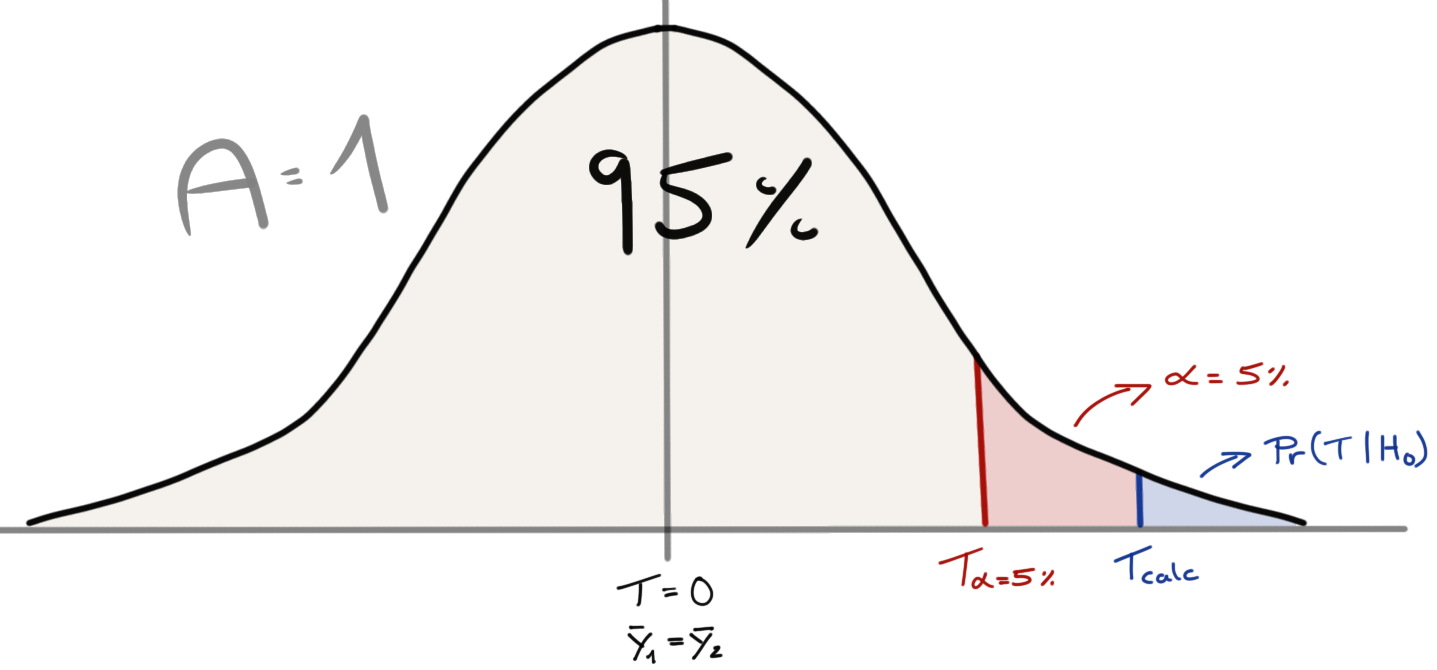
\includegraphics{./images/t-verteilung_01.png}

}

\caption{\label{fig-teststatistik-01}Die t-Verteilung aller möglichen
\(T_{calc}\) wenn die Nullhypothese wahr ist. Der Mittelwert der
t-Verteilun ist \(T=0\). Wenn wir keinen Effekt erwarten würden dann
wären die beiden Mittelwerte \(\bar{y}_1\) und \(\bar{y}_2\) gleich
groß. Die Differenz wäre 0. Je größer der \(T_{calc}\) wird desto
weniger können wir davon ausgehen, dass die beiden Mittelwerte gleich
sind. Liegt der \(T_{calc}\) über dem kritischen Wert von
\(T_{\alpha = 5\%}\) dann wir die Nullhypothese abgelehnt.}

\end{figure*}

In Abbildung~\ref{fig-teststatistik-01} ist die Verteilung aller
möglichen \(T_{calc}\) Werte unter der Annahme, dass die Nullhypothese
wahr ist, dargestellt. Wir sehen, dass die t-Verteilung am höchsten bei
\(T_{calc} = 0\) ist und niedrigeren Werte mit steigenden t-Werten
annimmt. Wenn \(T = 0\) dann sind auch die Mittelwerte gleich. Je größer
unsere berechnete Teststatistik \(T_{calc}\) wird, desto
unwahrscheinlicher ist es, dass die Nullhypothese gilt. Die t-Verteilug
ist so gebaut, dass die Fläche \(A\) unter der Kurve gleich \(A=1\) ist.
Wir können nun den kritschen Wert \(T_{\alpha = 5\%}\) berechnen an dem
rechts von dem Wert eine Fläche von 0.05 oder 5\% liegt. Sommit liegt
dann links von dem kritischen Wert die Fläche von 0.95 oder 95\%. Den
kritischen Wert \(T_{\alpha = 5\%}\) können wir statistischen Tabellen
entnehmen. Oder wir berechnen den kritischen Wert direkt in R mit
\(T_{\alpha = 5\%} = 2.78\).

Kommen wir zurück zu unserem Beispiel. Wir haben in unserem
Datenbeispiel für den Vergleich von der Sprungweite in {[}cm{]} von
Hunde- und Katzenflöhen eine Teststatistik von \(T_{calc} = 3.6\)
berechnet. Der kritische Wert um die Nullhypothese abzulehnen liegt bei
\(T_{\alpha = 5\%} = 2.78\). Wenn \(T_{calc} \geq T_{\alpha = 5\%}\)
wird die Nullhypothese (H\(_0\)) abgelehnt. In unserem Fall ist
\(3.6 \geq 2.78\). Wir können die Nullhypothese ablehnen. Es gibt einen
Unterschied zwischen der mittleren Sprungweite von Hunde- und
Katzenflöhen.

\begin{marginfigure}

{\centering 
\includegraphics[width=0.5\textwidth,height=\textheight]{./images/angel_01.png}

}

\end{marginfigure}

\emph{Es gibt einen Unterschied zwischen der mittleren Sprungweite von
Hunde- und Katzenflöhen.} Die Aussage ist \textbf{statistisch} falsch.
Wir können im frequentistischen Hypothesentesten keine Aussage über die
\(H_A\) treffen. Im Sinne der Anwendbarkeit soll es hier so stehen
bleiben.

Nun ist es leider so, dass jeder statistische Test seine eigene
Teststatistik \(T\) hat. Daher ist es etwas mühselig sich immer neue und
andere kritische Werte für jeden Test zu merken. Es hat sich daher
eingebürgert, sich nicht die Teststatistik für die Testentscheidung
gegen die Nullhypothese zu nutzen sondern den p-Wert. Den p-Wert wollen
wir uns in dem folgenden Abschnitt anschauen.

\begin{tcolorbox}[enhanced jigsaw, bottomrule=.15mm, toptitle=1mm, colbacktitle=quarto-callout-important-color!10!white, opacityback=0, bottomtitle=1mm, leftrule=.75mm, toprule=.15mm, breakable, rightrule=.15mm, title=\textcolor{quarto-callout-important-color}{\faExclamation}\hspace{0.5em}{Entscheidung mit der berechneten Teststatistik}, coltitle=black, colframe=quarto-callout-important-color-frame, colback=white, titlerule=0mm, left=2mm, arc=.35mm, opacitybacktitle=0.6]
Bei der Entscheidung mit der Teststatistik müssen wir zwei Fälle
unterschieden.

\begin{enumerate}
\def\labelenumi{(\arabic{enumi})}
\item
  Bei einem t-Test und einem \(\mathcal{X}^2\)-Test gilt, wenn
  \(T_{calc} \geq T_{\alpha = 5\%}\) wird die Nullhypothese (H\(_0\))
  abgelehnt.
\item
  Bei einem Wilcoxon-Mann-Whitney-Test gilt, wenn
  \(T_{calc} < T_{\alpha = 5\%}\) wird die Nullhypothese (H\(_0\))
  abgelehnt.
\end{enumerate}

\textbf{Achtung --} Wir nutzen die Entscheidung mit der Teststatistik
\emph{nur und ausschließlich} in der Klausur. In der praktischen
Anwendung hat die Betrachtung der berechneten Teststatistik \emph{keine}
Verwendung mehr.
\end{tcolorbox}

\hypertarget{sec-pwert}{%
\subsection*{\ldots{} anhand dem p-Wert}\label{sec-pwert}}
\addcontentsline{toc}{subsection}{\ldots{} anhand dem p-Wert}

\begin{tcolorbox}[enhanced jigsaw, bottomrule=.15mm, toptitle=1mm, colbacktitle=quarto-callout-tip-color!10!white, opacityback=0, bottomtitle=1mm, leftrule=.75mm, toprule=.15mm, breakable, rightrule=.15mm, title=\textcolor{quarto-callout-tip-color}{\faLightbulb}\hspace{0.5em}{Prinzip des statistischen Testens II - Der p-Wert}, coltitle=black, colframe=quarto-callout-tip-color-frame, colback=white, titlerule=0mm, left=2mm, arc=.35mm, opacitybacktitle=0.6]
Du findest auf YouTube \href{https://youtu.be/Zr8gdWZrSPc}{Prinzip des
statistischen Testens II - Der p-Wert} als Video Reihe. Ich werde zwar
alles nochmal hier als Text aufschreiben, aber manchmal ist das Sehen
und Hören dann einfacher.
\end{tcolorbox}

In dem vorherigen Abschnitt haben wir gelernt, wie wir zu einer
Entscheidung gegen die Nullhypothese anhand der Teststatistik kommen.
Wir haben einen kritischen Wert \(T_{\alpha = 5\%}\) definiert bei dem
rechts von dem Wert 5\% der Werte liegen. Anstatt nun den berechneten
Wert \(T_{calc}\) mit dem kritischen Wert \(T_{\alpha = 5\%}\) zu
vergleichen, vergleichen wir jetzt die Flächen rechts von den jeweiligen
Werten.

{\marginnote{\begin{footnotesize}Wir schreiben \(\boldsymbol{Pr}\) und
meinen damit eine Wahrscheinlichkeit (eng. \emph{probability}). Häufig
wird auch nur das \(P\) verwendet, aber dann kommen wir wieder mit
anderen Konzepten in die Quere.\end{footnotesize}}}

In Abbildung~\ref{fig-teststatistik-01} sind die Flächen auch
eingetragen. Da die gesamte Fläche unter der t-Verteilung mit \(A = 1\)
ist, können wir die Flächen auch als Wahrscheinlichkeiten lesen. Die
Fläche rechts von der berechneten Teststatistik \(T_{calc}\) wird
\(Pr(T_{calc}|H_0)\) oder \(p\)-Wert genannt. Die \emph{gesamte} Fläche
rechts von dem kritischen Wert \(T_{\alpha = 5\%}\) wird \(\alpha\)
genannt und liegt bei 5\%. Wir können also die Teststatistiken oder den
p-Wert mit dem \(\alpha\)-Niveau von 5\% vergleichen.

\hypertarget{tbl-t-und-A}{}
\begin{longtable}[]{@{}cc@{}}
\caption{\label{tbl-t-und-A}Zusammenhang zwischen der Teststatistik
\(T\) und der Fläche \(A\) rechts von der Teststatistik. Die Fläche
rechts von der berechneten Teststatistik \(T_{calc}\) wird \(Pr(T|H_0)\)
oder \(p\)-Wert genannt. Die Fläche rechts von dem kritischen Wert
\(T_{\alpha = 5\%}\) wird \(\alpha\) genannt und liegt bei
5\%.}\tabularnewline
\toprule()
Teststatistik \(T\) & Fläche \(A\) \\
\midrule()
\endfirsthead
\toprule()
Teststatistik \(T\) & Fläche \(A\) \\
\midrule()
\endhead
\(T_{calc}\) & \(Pr(T_{calc}|H_0)\) oder \(p\)-Wert \\
\(T_{\alpha = 5\%}\) & \(\alpha\) \\
\bottomrule()
\end{longtable}

Der p-Wert oder \(Pr(T|H_0)\) ist eine Wahrscheinlichkeit. Eine
Wahrscheinlichkeit kann die Zahlen von 0 bis 1 annehmen. Dabei sind die
Grenzen einfach zu definieren. Eine Wahrscheinlichkeit von \(Pr(A) = 0\)
bedeutet, dass das Ereignis A nicht auftritt; eine Wahrscheinlichkeit
von \(Pr(A) = 1\) bedeutet, dass das Ereignis A eintritt. Der Zahlenraum
dazwischen stellt jeden von uns schon vor große Herausforderungen. Der
Unterschied zwischen 40\% und 60\% für den Eintritt des Ereignisses A
sind nicht so klar zu definieren, wie du auf den ersten Blick meinen
magst.

Ein frequentistischer Hypothesentest beantwortet die Frage, mit welcher
Wahrscheinlichkeit \(Pr\) die Teststatistik \(T\) aus dem Experiment mit
den Daten \(D\) zu beobachten wären, wenn es keinen Effekt gäbe (\(H_0\)
ist wahr).

{\marginnote{\begin{footnotesize}\textbf{Likelihood} heißt Plausibilität
und \textbf{Probability} heißt Wahrscheinlichkeit.\end{footnotesize}}}

Im Englischen gibt es die Begrifflichkeiten einer \emph{Likelihood} und
einer \emph{Probability} in der Statistik. Meist wird beides ins
Deutsche ungenau mit Wahrscheinlichkeit übersetzt oder wir nutzen
einfach \emph{Likelihood}. Was aber auch nicht so recht weiterhilft. Es
handelt sich hierbei aber um zwei unterschiedliche Konzepte. Deshalb
Übersetzen wir \emph{Likelihood} mit Plausibilität und
\emph{Probability} mit Wahrscheinlichkeit.

Im Folgenden berechnen wir den \(p\)-Wert in R mit der Funktion
\texttt{t.test()}. Mehr dazu im Kapitel~\ref{sec-ttest}, wo wir den
t-Test und deren Anwendung im Detail besprechen.

\begin{verbatim}
# A tibble: 1 x 2
  statistic p.value
      <dbl>   <dbl>
1      2.81  0.0309
\end{verbatim}

{\marginnote{\begin{footnotesize}Wir sagen, dass wir ein
\textbf{signifikantes} Ergebnis haben, wenn der \(p\)-Wert kleiner ist
als die Signifikanzschwelle \(\alpha\) von 5\%.\end{footnotesize}}}

Wir erhalten einen \(p\)-Wert von 0.031 und vergleichen diesen Wert zu
einem \(\alpha\) von 5\%. Ist der \(p\)-Wert kleiner als der
\(\alpha\)-Wert von 5\%, dann können wir die Nullhypothese ablehnen. Da
0.031 kleiner ist als 0.05 können wir die Nullhypothese und damit die
Gleichheit der mittleren Sprungweiten in {[}cm{]} ablehnen. Wir sagen,
dass wir ein signifikantes Ergebnis vorliegen haben.

\begin{tcolorbox}[enhanced jigsaw, bottomrule=.15mm, toptitle=1mm, colbacktitle=quarto-callout-important-color!10!white, opacityback=0, bottomtitle=1mm, leftrule=.75mm, toprule=.15mm, breakable, rightrule=.15mm, title=\textcolor{quarto-callout-important-color}{\faExclamation}\hspace{0.5em}{Entscheidung mit dem p-Wert}, coltitle=black, colframe=quarto-callout-important-color-frame, colback=white, titlerule=0mm, left=2mm, arc=.35mm, opacitybacktitle=0.6]
Wenn der p-Wert \(\leq \alpha\) dann wird die Nullhypothese (H\(_0\))
abgelehnt. Das Signifikanzniveau \(\alpha\) wird als Kulturkonstante auf
5\% oder 0.05 gesetzt. Die Nullhypothese (H\(_0\)) kann auch
Gleichheitshypothese gesehen werden. Wenn die H\(_0\) gilt, liegt kein
Unterschied zwischen z.B. den Behandlungen vor.
\end{tcolorbox}

\hypertarget{sec-ki}{%
\subsection*{\ldots{} anhand des 95\% Konfidenzintervall}\label{sec-ki}}
\addcontentsline{toc}{subsection}{\ldots{} anhand des 95\%
Konfidenzintervall}

Ein statistischer Test der eine Teststatistik \(T\) berechnet liefert
auch immer einen \(p\)-Wert. Nicht alle statistischen Tests ermöglichen
es ein 95\% Konfidenzintervall zu berechnen. Abbildung~\ref{fig-ki-00}
zeigt ein 95\% konfidenzintervall.

\begin{figure}

{\centering 
\includegraphics[width=0.7\textwidth,height=\textheight]{./images/ci-00.png}

}

\caption{\label{fig-ki-00}Ein 95\% Konfidenzintervall. Der Punkt in der
Mitte entspricht dem Unterschied oder Effekt \(\Delta\).}

\end{figure}

{\marginnote{\begin{footnotesize}Mit \textbf{p-Werten} haben wir
Wahrscheinlichkeitsaussagen und damit über die \textbf{Signifikanz}.
Damit haben wir noch keine Aussage über die \textbf{Relevanz} des
beobachtenten Effekts.\end{footnotesize}}}

Mit der Teststatistik \(T\) und dem damit verbundenen \(p\)-Wert haben
wir uns \emph{Wahrscheinlichkeiten} angeschaut und erhalten eine
\emph{Wahrscheinlichkeitsaussage}. Eine Wahrscheinlichkeitsaussage sagt
aber nichts über den Effekt \(\Delta\) aus. Also wie groß ist der
mittlere Sprung\emph{unterschied} zwischen Hunde- und Katzenflöhen. Eine
nährere betrachtung von dem Effekt in der Statistik findest du in
\textbf{?@sec-effect}.

Die Idee von 95\% Kondifenzintervallen ist es jetzt den Effekt mit der
Wahrscheinlichkeitsaussage zusammenzubringen und beides in einer
\emph{Visualisierung} zu kombinieren. Im Folgenden sehen wir die
vereinfachte Formel für das 95\% Konfidenzintervall eines t-Tests.

\[
\left[
(\bar{y}_1-\bar{y}_2) - 
T_{\alpha = 5\%} \cdot \frac {s_p}{\sqrt{n}}; \;
(\bar{y}_1-\bar{y}_2) + 
T_{\alpha = 5\%} \cdot \frac {s_p}{\sqrt{n}};
\right]
\]

Die Formel ist ein wenig komplex, aber im Prinzip einfach. Der linke und
der rechte Teil neben dem Semikolon sind fast gleich, bis auf das Plus-
und Minuszeichen. Abbildung~\ref{fig-ki-01} visualisert die Formel
einmal. Wir sehen Folgendes in der Formel und dann in der entsprechenden
Abbildung:

\begin{itemize}
\tightlist
\item
  \((\bar{y}_{1}-\bar{y}_{2})\) ist der Effekt \(\Delta\). In diesem
  Fall der Mittelwertsunterschied. Wir finden den Effekt als Punkt in
  der Mitte des Intervals.
\item
  \(T_{\alpha = 5\%} \cdot \frac {s}{\sqrt{n}}\) ist der Wert, der die
  Arme des Intervals bildet. Wir vereinfachen die Formel mit \(s_p\) für
  die gepoolte Standardabweichung und \(n_g\) für die Fallzahl der
  beiden Gruppen. Wir nehmen an das beide Gruppen die gleiche Fallzahl
  \(n_1 = n_2\) haben.
\end{itemize}

\begin{figure}

{\centering \includegraphics[width=1\textwidth,height=\textheight]{./images/ci-01.png}

}

\caption{\label{fig-ki-01}Zusammenhang zwischen der vereinfachten Formel
für das 95\% Konfidenzintervall und der Visualisierung des 95\%
Konfidenzintervalls. Der Effektschätzer wird als Punkt in der Mitte des
Intervalls dargestellt. Der Effektschäter \(\Delta\) kann entweder ein
Mittelwertsunterschied sein oder ein Anteilsunterschied. Bei einem
Mittelwertsunterschied kann die Nullhypothese abgelehnt werden, wenn die
0 nicht im Konfidenzintervall ist; bei einem Anteilsunterschied wenn die
1 nicht im Konfidenzintervall ist. Die Arme werden länger oder kürzer je
nachdem wie sich die statistischen Maßzahlen \(s\) und \(n\) verändern.}

\end{figure}

{\marginnote{\begin{footnotesize}Die Funktion \texttt{factor()} in R
erlaubt es dir die Level eines Faktors zu sortieren und so festzulegen
ob Level \texttt{cat} minus Level \texttt{dog} oder umgekehrt von R
gerechnet wird.\end{footnotesize}}}

Wir können eine biologische Relevanz definieren, dadurch das ein 95\%
Konfidenzintervall die Wahrscheinlichkeitsaussage über die Signifkanz,
daher ob die Nullhypothese abgelehnt werden kann, mit dem Effekt
zusammenbringt. Wo die Signifikanzschwelle klar definiert ist, hängt die
Relevanzschwelle von der wissenschaftlichen Fragestellung und weiteren
externen Faktoren ab. Die Signifikanzschwelle liegt bei 0, wenn wir
Mittelwerte miteinander vergleichen und bei 1, wenn wir Anteile
vergleichen. Abbildung~\ref{fig-relevanz} zeigt fünf 95\%
Konfidenzintervalle (a-e), die sich anhand der Signifikanz und Relevanz
unterscheiden. Bei der Relevanz ist es wichtig zu wissen in welche
\emph{Richtung} der Effekt gehen soll. Erwarten wir einen positiven
Effekt wenn wir die Differenz der beiden Gruppen bilden oder einen
negativen Effekt?

\begin{figure}

{\centering \includegraphics{./images/ci-02.png}

}

\caption{\label{fig-relevanz}Verschiedene signifikante und relevante
Konfidenzintervalle: (a) nicht signifikant und nicht relevant; (b)
signifikant und nicht relevant; (c) signifikant und relevant; (d)
signifikant und nicht relevant, der Effekt ist zu klein; (e) signifikant
und potenziell relevant, Effekt zeigt in eine unerwartete Richtung
gegeben der Relevanzschwelle.}

\end{figure}

Wir wollen uns nun einmal anschauen, wie sich ein 95\%
Konfidenzintervall berechnet. Wir nehmen dafür die vereinfachte Formel
und setzen die berechneten statistischen Maßzahlen ein. In der Anwendung
werden wir die Konfidenzintervalle nicht selber berechnen. Wenn ein
statistisches Verfahren konfidenzintervalle berechnen kann, dann liefert
die entsprechende Funktion in R das Konfidenzintervall.

Es ergibt sich Folgende ausgefüllte, vereinfachte Formel für das 95\%
Konfidenzintervalls eines t-Tests für das Beispiel des
Sprungweitenunterschieds {[}cm{]} zwischen Hunde- und Katzenflöhen.

\begin{marginfigure}

{\centering \includegraphics[width=0.5\textwidth,height=\textheight]{./images/angel_01.png}

}

\end{marginfigure}

Wir nutzen hier eine \textbf{vereinfachte Formel} für das
Konfidenzintervall um das Konzept zu verstehen. Später berechnen wir das
Konfidenzintervall in R.

\[
\left[
(9.2-7.8) - 
2.78 \cdot \frac {0.55}{\sqrt{4}}; \;
(9.2-7.8) + 
2.78 \cdot \frac {0.55}{\sqrt{4}};
\right]
\]

mit

\begin{itemize}
\tightlist
\item
  \(\bar{y}_{cat} = 9.2\) dem Mittelwert für die Gruppe \emph{cat}.
\item
  \(\bar{y}_{dog} = 7.8\) dem Mittelwert für die Gruppe \emph{dog}.
\item
  \(T_{\alpha = 5\%} = 2.78\) dem kritischen Wert.
\item
  \(s_p = 0.55\) der gepoolten Standardabweichung mit
  \(s_p = \tfrac{0.6 + 0.5}{2}\).
\item
  \(n_g = 4\) der Gruppengröße der Gruppe A und B. Wir nehmen an beide
  Gruppen sind gleich groß.
\end{itemize}

Lösen wir die Formel auf, so ergibt sich folgendes 95\%
Konfidenzintervall des Mittelwertsunterschiedes der Hunde- und
Katzenflöhe.

\[[0.39; 2.20]\]

Wir können sagen, dass mit 95\% Wahrscheinlichkeit das
Konfidenzintervall den wahren Effektunterschied \(\Delta\) überdeckt.
Oder etwas mehr in Prosa, dass wir eine Sprungweiten\emph{unterschied}
von 0.39 cm bis 2.20 cm zwischen Hunde- und Katzenflöhen erwarten
würden.

Die Entscheidung gegen die Nullhypothese bei einem
Mittelwertsunterschied erfolgt bei einem 95\% Konfidenzintervall danach
ob die Null mit im Konfidenzintervall liegt oder nicht. In dem Interval
\([0.39; 2.20]\) ist die Null nicht enthalten, also können wir die
Nullhypothese ablehnen. Es ist mit einem Unterschied zwischen den
mittleren Sprungweiten von Hunde- und Katzenflöhen auszugehen.

In unserem Beispiel, könnten wir die Relevanzschwelle für den mittleren
Sprungweitenunterschied zwischen Hund- und Katzenflöhen auf 2 cm setzen.
In dem Fall würden wir entscheiden, dass der mittlere
Sprungweitenunterschied nicht relevant ist, da die 2 cm im
Konfidenzintervall enthalten sind. Was wäre wenn wir die
Relevanzschwelle auf 4 cm setzen? Dann wäre zwar die Relevanzschwelle
nicht mehr im Konfidenzintervall, aber wir hätten Fall (d) in der
Abbildung~\ref{fig-relevanz} vorliegen. Der Effekt ist einfach zu klein,
dass der Effekt relevant sein könnte.

\begin{tcolorbox}[enhanced jigsaw, bottomrule=.15mm, toptitle=1mm, colbacktitle=quarto-callout-important-color!10!white, opacityback=0, bottomtitle=1mm, leftrule=.75mm, toprule=.15mm, breakable, rightrule=.15mm, title=\textcolor{quarto-callout-important-color}{\faExclamation}\hspace{0.5em}{Entscheidung mit dem 95\% Konfidenzintervall}, coltitle=black, colframe=quarto-callout-important-color-frame, colback=white, titlerule=0mm, left=2mm, arc=.35mm, opacitybacktitle=0.6]

Bei der Entscheidung mit dem 95\% Konfidenzinterval müssen wir zwei
Fälle unterscheiden.

\begin{enumerate}
\def\labelenumi{(\arabic{enumi})}
\item
  Entweder schauen wir uns einen Mittelwertsunterschied
  (\(\Delta_{y_1-y_2}\)) an, dann können wir die Nullhypothese (H\(_0\))
  \emph{nicht} ablehnen, wenn die \textbf{0} im 95\% Konfidenzinterval
  ist.
\item
  Oder wir schauen uns einen Anteilsunterschied (\(\Delta_{y_1/y_2}\))
  an, dann können wir die Nullhypothese (H\(_0\)) \emph{nicht} ablehnen,
  wenn die \textbf{1} im 95\% Konfidenzinterval ist.
\end{enumerate}

\end{tcolorbox}

\hypertarget{auswirkung-des-effektes-der-streuung-und-der-fallzahl}{%
\section*{Auswirkung des Effektes, der Streuung und der
Fallzahl}\label{auswirkung-des-effektes-der-streuung-und-der-fallzahl}}
\addcontentsline{toc}{section}{Auswirkung des Effektes, der Streuung und
der Fallzahl}

Wir wollen einmal den Zusammenhang zwischen dem Effekt \(\Delta\), der
Streuung als Standardabweichung \(s\) und Fallzahl \(n\) uns näher
anschauen. Wir können die Formel des t-Tests wie folgt vereinfachen.

\[
T_{calc}=\cfrac{\bar{y}_1-\bar{y}_1}{s_{p} \cdot \sqrt{2/n_g}}
\]

Für die Betrachtung der Zusammenhänge wandeln wir \(\sqrt{2/n_g}\) in
\(1/n\) um. Dadurch wandert die Fallzahl \(n\) in den Zähler. Die
Standardabweichung verallgemeinern wir zu \(s\) und damit allgemein zur
Streuung. Abschließend betrachten wir \(\bar{y}_A-\bar{y}_B\) als den
Effekt \(\Delta\). Es ergibt sich folgende vereinfachte Formel.

\[
T_{calc} = \cfrac{\Delta \cdot n}{s}
\]

Wir können uns nun die Frage stellen, wie ändert sich die Teststatistik
\(T_{calc}\) in Abhängigkeit vom Effekt \(\Delta\), der Fallzahl \(n\)
und der Streuung \(s\) in den Daten. Die Tabelle~\ref{tbl-t-und-p} zeigt
die Zusammenhänge auf. Die Aussagen in der Tabelle lassen sich
generalisieren. So bedeutet eine steigende Fallzahl meist mehr
signifikante Ergebnisse. Eine stiegende Streuung reduziert die
Signifikanz eines Vergleichs. Ein Ansteigen des Effektes führt zu mehr
signifikanten Ergebnissen. Ebenso verschiebt eine Veränderung des Effekt
das Konfidenzintervall, eine Erhöhung der Streuung macht das
konfidenzintervall breiter, eine sinkende Streeung macht das
konfidenzintervall schmaller. bei der Fallzahl verhält es sich
umgekehrt. Eine Erhöhung der Fallzahl macht das Konfidenzintervall
schmaller und eine sinkende Fallzahl das Konfidenzintervall breiter.

\begin{figure*}

\hypertarget{tbl-t-und-p}{}
\begin{longtable}[]{@{}
  >{\centering\arraybackslash}p{(\columnwidth - 14\tabcolsep) * \real{0.0950}}
  >{\centering\arraybackslash}p{(\columnwidth - 14\tabcolsep) * \real{0.1250}}
  >{\centering\arraybackslash}p{(\columnwidth - 14\tabcolsep) * \real{0.1900}}
  >{\raggedright\arraybackslash}p{(\columnwidth - 14\tabcolsep) * \real{0.0850}}
  >{\centering\arraybackslash}p{(\columnwidth - 14\tabcolsep) * \real{0.1050}}
  >{\centering\arraybackslash}p{(\columnwidth - 14\tabcolsep) * \real{0.1250}}
  >{\centering\arraybackslash}p{(\columnwidth - 14\tabcolsep) * \real{0.1900}}
  >{\raggedright\arraybackslash}p{(\columnwidth - 14\tabcolsep) * \real{0.0850}}@{}}
\caption{\label{tbl-t-und-p}Zusammenhang von der Teststatistik
\(T_{calc}\) und dem p-Wert \(Pr(\geq T_{calc}|H_0)\) sowie dem
\(KI_{1-\alpha}\) in Abhängigkeit vom Effekt \(\Delta\), der Fallzahl
\(n\) und der Streuung \(s\).}\tabularnewline
\toprule()
\begin{minipage}[b]{\linewidth}\centering
\end{minipage} & \begin{minipage}[b]{\linewidth}\centering
\(\boldsymbol{T_{calc}}\)
\end{minipage} & \begin{minipage}[b]{\linewidth}\centering
\(\boldsymbol{Pr(\geq T_{calc}|H_0)}\)
\end{minipage} & \begin{minipage}[b]{\linewidth}\raggedright
\(KI_{1-\alpha}\)
\end{minipage} & \begin{minipage}[b]{\linewidth}\centering
\end{minipage} & \begin{minipage}[b]{\linewidth}\centering
\(\boldsymbol{T_{calc}}\)
\end{minipage} & \begin{minipage}[b]{\linewidth}\centering
\(\boldsymbol{Pr(\geq T_{calc}|H_0)}\)
\end{minipage} & \begin{minipage}[b]{\linewidth}\raggedright
\(KI_{1-\alpha}\)
\end{minipage} \\
\midrule()
\endfirsthead
\toprule()
\begin{minipage}[b]{\linewidth}\centering
\end{minipage} & \begin{minipage}[b]{\linewidth}\centering
\(\boldsymbol{T_{calc}}\)
\end{minipage} & \begin{minipage}[b]{\linewidth}\centering
\(\boldsymbol{Pr(\geq T_{calc}|H_0)}\)
\end{minipage} & \begin{minipage}[b]{\linewidth}\raggedright
\(KI_{1-\alpha}\)
\end{minipage} & \begin{minipage}[b]{\linewidth}\centering
\end{minipage} & \begin{minipage}[b]{\linewidth}\centering
\(\boldsymbol{T_{calc}}\)
\end{minipage} & \begin{minipage}[b]{\linewidth}\centering
\(\boldsymbol{Pr(\geq T_{calc}|H_0)}\)
\end{minipage} & \begin{minipage}[b]{\linewidth}\raggedright
\(KI_{1-\alpha}\)
\end{minipage} \\
\midrule()
\endhead
\(\Delta \uparrow\) & steigt & sinkt & verschoben &
\(\Delta \downarrow\) & sinkt & steigt & verschoben \\
\(s \uparrow\) & sinkt & steigt & breiter & \(s \downarrow\) & steigt &
sinkt & schmaller \\
\(n \uparrow\) & steigt & sinkt & schmaller & \(n \downarrow\) & sinkt &
steigt & breiter \\
\bottomrule()
\end{longtable}

\end{figure*}

\hypertarget{testtheorie}{%
\section*{Testtheorie}\label{testtheorie}}
\addcontentsline{toc}{section}{Testtheorie}

\begin{tcolorbox}[enhanced jigsaw, bottomrule=.15mm, toptitle=1mm, colbacktitle=quarto-callout-tip-color!10!white, opacityback=0, bottomtitle=1mm, leftrule=.75mm, toprule=.15mm, breakable, rightrule=.15mm, title=\textcolor{quarto-callout-tip-color}{\faLightbulb}\hspace{0.5em}{Prinzip der statistischen Testentscheidung - H\(_0\) und H\(_A\)}, coltitle=black, colframe=quarto-callout-tip-color-frame, colback=white, titlerule=0mm, left=2mm, arc=.35mm, opacitybacktitle=0.6]
Du findest auf YouTube \href{https://youtu.be/ttkGnexSXHw}{Prinzip der
statistischen Testentscheidung - \(H_0\) und \(H_A\)} als Video Reihe.
Ich werde zwar alles nochmal hier als Text aufschreiben, aber manchmal
ist das Sehen und Hören dann einfacher.
\end{tcolorbox}

Vielleicht ist die Idee der Testentscheidung besser mit der Analogie des
Rauchmelders zu verstehen. Wir nehmen an, dass der Rauchmelder der
statistische Test ist. Der Rauchmelder hängt an der Decke und soll
entscheiden, ob es brennt oder nicht. Daher muss der Rauchmelder
entscheiden, die Nullhypothese ``kein Feuer'' abzulehnen oder die
Hypothese ``kein Feuer'' beizubehalten.

\begin{align*} 
H_0&: \mbox{kein Feuer im Haus} \\  
H_A&: \mbox{Feuer im Haus} \\   
\end{align*}

Wir können jetzt den Rauchmelder einstellen, so dass der Rauchmelder bei
einer Kerze losgeht oder erst bei einem Stubenbrand. Wie sensibel auf
Rauch wollen wir den Rauchmelder einstellen? Soll der Rauchmelder sofort
die Nullhypothese ablehnen? Wenn also nur eine Kerze brennt. Soll also
der \(\alpha\)-Fehler groß sein? Das wäre nicht sehr sinnvoll. Due
Feuerwehr würde schon bei einer Kerze kommen oder wenn wir mal was
anbrennen. Wir dürfen also den \(\alpha\)-Fehler nicht zu groß
einstellen.

Intuitiv würde man meinen, ein sehr kleiner \(\alpha\)-Fehler nun
sinnvoll sei. Wenn wir aber den Rauchmelder sehr unsensibel einstellen,
also der Rauchmelder erst bei sehr viel Rauch die Nullhypothese ablehnt,
könnte das Haus schon unrettbar in Flammen stehen. Dieser Fehler, Haus
steht in Flammen und der Rauchmelder geht nicht, wird als
\(\beta\)-Fehler bezeichnet. Wie du siehst hängen die beiden Fehler
miteinander zusammen. Wichtig hierbei ist immmer, dass wir uns einen
Zustand vorstellen, das Haus brent nicht (\(H_0\) ist wahr) oder das
Haus brennt nicht (\(H_A\) ist wahr). An diesem Zustand entscheiden wir
dann, wie hoch der Fehler jeweils sein soll diesen Zustand zu übersehen.

\begin{tcolorbox}[enhanced jigsaw, bottomrule=.15mm, toptitle=1mm, colbacktitle=quarto-callout-note-color!10!white, opacityback=0, bottomtitle=1mm, leftrule=.75mm, toprule=.15mm, breakable, rightrule=.15mm, title=\textcolor{quarto-callout-note-color}{\faInfo}\hspace{0.5em}{Der \(\alpha\)-Fehler und \(\beta\)-Fehler als Rauchmelderanalogie}, coltitle=black, colframe=quarto-callout-note-color-frame, colback=white, titlerule=0mm, left=2mm, arc=.35mm, opacitybacktitle=0.6]

Häufig verwirrt die etwas theoretische Herangehensweise an den
\(\alpha\)-Fehler und \(\beta\)-Fehler. Wir versuchen hier nochmal die
Analogie eines Rauchmelders und dem Feuer im Haus.

\begin{figure}

{\centering \includegraphics[width=0.8\textwidth,height=\textheight]{./images/t-verteilung_05.png}

}

\caption{\label{fig-teststatistik-05}Andere Art der Darstellung des
\(\alpha\)-Fehlers als \emph{Alarm without fire} und dem
\(\beta\)-Fehler als \emph{Fire without alarm}. Je nachdem wie
empfindlich wir den Alarm des Rauchmelders (den statistischen Test) über
das \(\alpha\) einstellen, desto mehr Alarm bekommen wir ohne das ein
Effekt vorhanden wäre. Drehen wir den Alarm zu niedrig, dann kriegen wir
kein Feuer mehr angezeigt, den \(\beta\)-Fehler.}

\end{figure}

\begin{itemize}
\tightlist
\item
  \(\boldsymbol{\alpha}\)\textbf{-Fehler}: Alarm without fire. Der
  statistische Test schlägt Alarm und wir sollen die \(H_0\) ablehnen,
  obwohl die \(H_0\) in Wahrheit gilt und kein Effekt vorhanden ist.
\item
  \(\boldsymbol{\beta}\)\textbf{-Fehler}: Fire without alarm. Der
  statistische Test schlägt \emph{nicht} an und wir sollen die \(H_0\)
  beibehalten, obwohl die \(H_0\) in Wahrheit \emph{nicht} gilt und
  \emph{ein} Effekt vorhanden ist.
\end{itemize}

\end{tcolorbox}

Wie sieht nun die Lösung, erstmal für unseren Rauchmelder, aus? Wir
müssen Grenzen für den \(\alpha\) und \(\beta\)-Fehler festlegen.

{\marginnote{\begin{footnotesize}\textbf{Wir setzen den}
\(\alpha\)-Fehler auf 5\%.\end{footnotesize}}}

\begin{itemize}
\tightlist
\item
  Wir setzen den \(\alpha\)-Fehler auf 5\%. Somit haben wir in 1 von 20
  Fällen das Problem, dass uns der Rauchmelder angeht obwohl gar kein
  Feuer da ist. Wir lehnen die Nullhypothese ab, obwohl die
  Nullhypothese gilt.
\end{itemize}

{\marginnote{\begin{footnotesize}\textbf{Wir setzen den}
\(\beta\)-Fehler auf 20\%.\end{footnotesize}}}

\begin{itemize}
\tightlist
\item
  Auf der anderen Seite setzen wir den \(\beta\)-Fehler auf 20\%. Damit
  brennt uns die Bude in 1 von 5 Fällen ab ohne das der Rauchmelder
  einen Pieps von sich gibt. Wir behalten die Nullhypothese bei, obwohl
  die Nullhypothese nicht gilt.
\end{itemize}

Nachdem wir uns die Testentscheidung mit der Analogie des Rauchmelders
angesehen haben, wollen wir uns wieder der Statistik zuwenden.
Betrachten wir das Problem nochmal von der theoretischen Seite mit den
statistischen Fachbegriffen.

Soweit haben wir es als gegeben angesehen, dass wir eine
Testentscheidung durchführen. Entweder mit der Teststatistik, dem
\(p\)-Wert oder dem 95\% Konfidenzintervall. Immer wenn wir eine
Entscheidung treffen, können wir auch immer eine falsche Entscheidung
treffen. Wie wir wissen hängt die berechnete Teststatistik \(T_{calc}\)
nicht nur vom Effekt \(\Delta\) ab sondern auch von der Streuung \(s\)
und der Fallzahl \(n\). Auch können wir den falschen Test wählen oder
Fehler im Design des Experiments gemacht haben. Schlussendlich gibt es
viele Dinge, die unsere \emph{simple} mathematischen Formeln
beeinflussen können, die wir nicht kennen. Ein frequentistischer
Hypothesentest gibt immer nur eine Aussage über die Nullhypothese
wieder. Also ob wir die Nullhypothese ablehnen können oder nicht.

Abbildung~\ref{fig-teststatistik-03} zeigt die theoretische Verteilung
der Nullyhypothese und der Alternativehypothese. Wenn die beiden
Verteilungen sehr nahe beieinander sind, wird es schwer für den
statistischen Test die Hypothesen klar voneinander zu trennen. Die
Verteilungen überlappen. Es gibt einen sehr kleinen Unterschied in den
Sprungweiten zwischen Hunde- und Katzenflöhen.

\begin{figure*}

{\centering \includegraphics{./images/t-verteilung_03.png}

}

\caption{\label{fig-teststatistik-03}Darstellung der Null- und
Alternativehypothese. Mit steigendem \(T_{calc}\) wird die
Wahrscheinlichkeit für die \(H_0\) immer kleiner. Leider ist uns nichts
über \(H_A\) und deren Lage bekannt. Sollte die \(H_A\) Verteilung zu
weit nach links ragen, könnten wir die \(H_0\) beibehalten, obwohl die
\(H_A\) gilt.}

\end{figure*}

{\marginnote{\begin{footnotesize}\textbf{Achtung} In der Regression wird
uns auch wieder das \(\beta\) als Symbol begegnen. In der
\emph{statistischen Testtheorie} ist das \(\beta\) ein Fehler; in der
Regression ist das \(\beta\) ein Koeffizient der Regression. Hier ist
der Kontext wichtig.\end{footnotesize}}}

Wir können daher bei statistischen Testen zwei Arten von Fehlern machen.
Zum einen den \(\alpha\) Fehler oder auch Type I Fehler genannt. Zum
anderen den \(\beta\) Fehler oder auch Type II Fehler genannt. Die
Grundidee basiert darauf, dass wir eine Testentscheidung gegen die
Nullhypothese machen. Diese Entscheidung kann richtig sein, da in
Wirklichkeit die Nullhypothese gilt oder aber falsch sein, da in
Wirklichkeit die Nullhypothese nicht gilt. In
Abbildung~\ref{fig-teststatistik-04} wird der Zusammenhang in einer 2x2
Tafel veranschaulicht.

\begin{figure*}

{\centering \includegraphics{./images/t-verteilung_04.png}

}

\caption{\label{fig-teststatistik-04}Zusammenhang zwischen der
Testentscheidung gegen die \(H_0\) Hypothese sowie dem Beibehalten der
\(H_0\) Hypothese und der unbekannten Wahrheit in der die \(H_0\) falsch
sein kann oder die \(H_0\) wahr sein kann. Wir können mit unserer
Testenstscheidung richtig liegen oder falsch. Mit welcher
Wahrscheinlichkeit geben der \(\alpha\) Fehler und \(\beta\) Fehler
wieder. Unten rechts ist der Zusammenhang zu der
Abbildung~\ref{fig-teststatistik-03} gezeigt.}

\end{figure*}

\marginnote{\begin{footnotesize}

Die Diskussion über den \(p\)-Wert und dem Vergleich mit dem
\(\alpha\)-Fehler wird in der Statistik seit 2019 verstärkt diskutiert
(Wasserstein, Schirm, und Lazar 2019). Das Nullritual wird schon lamge
kritisiert (Gigerenzer, Krauss, und Vitouch 2004). Siehe dazu auch
\href{https://www.tandfonline.com/toc/utas20/73/sup1}{The American
Statistician, Volume 73, Issue sup1 (2019)}.

\end{footnotesize}}

Beide Fehler sind Kulturkonstanten. Das heißt, dass sich diese Zahlen
von 5\% und 20\% so ergeben haben. Es gibt keinen rationalen Grund diese
Zahlen so zu nehmen. Man kann eigentlich sagen, dass die 5\% und die
20\% eher einem Zufall entsprungen sind, als einer tieferen Rationalen.
Wir behalten diese beiden Zahlen bei aus den beiden schlechtesten Gründe
überhaupt: i) es wurde schon immer so gemacht und ii) viele machen es
so.

Eine weitere wichtige statistische Maßzahl im Kontext der Testtheorie
ist die \(Power\) oder auch \(1-\beta\). Die \(Power\) ist die
Gegenwahrscheinlichkeit von dem \(\beta\)-Fehler. In der Analogie des
Rauchmelders wäre die \(Power\) daher \emph{Alarm with fire}. Das heißt,
wie wahrscheinlich ist es einen wahren Effekt - also einen Unterschied -
mit dem statistischen Test auch zu finden. Oder anders herum, wenn wir
wüssten, dass die Hunde- und Katzenflöhe unterschiedliche weit springen,
mit welcher Wahrscheinlichkeit würde diesen Unterschied ein
statistsicher Test auch finden? Mit eben der \(Power\), also gut 80\%.
Tabelle~\ref{tbl-power} zeigt die Abhängigkeit der \(Power\) vom Effekt
\(\Delta\), der Streuung \(s\) und der Fallzahl \(n\).

{\marginnote{\begin{footnotesize}Die \(Power\) ist eine
Wahrscheinlichkeit und sagt \emph{nichts} über die Relevanz des Effektes
aus.\end{footnotesize}}}

\hypertarget{tbl-power}{}
\begin{longtable}[]{@{}
  >{\centering\arraybackslash}p{(\columnwidth - 6\tabcolsep) * \real{0.1827}}
  >{\centering\arraybackslash}p{(\columnwidth - 6\tabcolsep) * \real{0.3077}}
  >{\centering\arraybackslash}p{(\columnwidth - 6\tabcolsep) * \real{0.2019}}
  >{\centering\arraybackslash}p{(\columnwidth - 6\tabcolsep) * \real{0.3077}}@{}}
\caption{\label{tbl-power}Abhängigkeit der \(Power (1-\beta)\) vom
Effekt \(\Delta\), der Fallzahl \(n\) und der Streuung \(s\). Die
\(Power\) ist eine Wahrscheinlichkeit und sagt nichts über die Relevanz
des Effektes aus.}\tabularnewline
\toprule()
\begin{minipage}[b]{\linewidth}\centering
\end{minipage} & \begin{minipage}[b]{\linewidth}\centering
\(\boldsymbol{Power (1-\beta)}\)
\end{minipage} & \begin{minipage}[b]{\linewidth}\centering
\end{minipage} & \begin{minipage}[b]{\linewidth}\centering
\(\boldsymbol{Power (1-\beta)}\)
\end{minipage} \\
\midrule()
\endfirsthead
\toprule()
\begin{minipage}[b]{\linewidth}\centering
\end{minipage} & \begin{minipage}[b]{\linewidth}\centering
\(\boldsymbol{Power (1-\beta)}\)
\end{minipage} & \begin{minipage}[b]{\linewidth}\centering
\end{minipage} & \begin{minipage}[b]{\linewidth}\centering
\(\boldsymbol{Power (1-\beta)}\)
\end{minipage} \\
\midrule()
\endhead
\(\Delta \uparrow\) & steigt & \(\Delta \downarrow\) & sinkt \\
\(s \uparrow\) & sinkt & \(s \downarrow\) & steigt \\
\(n \uparrow\) & steigt & \(n \downarrow\) & sinkt \\
\bottomrule()
\end{longtable}

\hypertarget{einseitig-oder-zweiseitig}{%
\subsection*{Einseitig oder
zweiseitig?}\label{einseitig-oder-zweiseitig}}
\addcontentsline{toc}{subsection}{Einseitig oder zweiseitig?}

Manchmal kommt die Frage auf, ob wir \emph{einseitig} oder
\emph{zweiseitig} einen statistischen Test durchführen wollen. Beim Fall
des zweiseitigen Testens verteilen wir den \(\alpha\)-Fehler auf beide
Seiten der Testverteilung mit jeweils \(\cfrac{\alpha}{2}\). In dem Fall
des einseitigen Tests liegt der gesamte \(\alpha\)-Fehler auf der
rechten \emph{oder} linken Seite der Testverteilung. In
Abbildung~\ref{fig-teststatistik-02} wird der Zusammenhang beispielhaft
an der t-Verteilung gezeigt.

\begin{figure*}

{\centering \includegraphics{./images/t-verteilung_02.png}

}

\caption{\label{fig-teststatistik-02}Zusammenhang zwischen dem
einseitigen und zweiseitigen Testen. Im Falle des zweiseitigen Testens
teilen wir den \(\alpha\)-Fehler auf beide Seiten der beispielhaften
t-Verteilung auf. Im Falle des einseitigen Testen leigt der gesamte
\(\alpha\)-Fehler auf der rechten \emph{oder} der linken Seite der
t-Verteilung.}

\end{figure*}

{\marginnote{\begin{footnotesize}In der Anwendung testen wir immer
zweiseitig.\end{footnotesize}}}

In der Anwendung testen wir immer zweiseitig. Der Grund ist, dass das
Vorzeichen von der Teststatik davon abhängt, welche der beiden Gruppen
den größeren Mittelwert hat. Da wir die Mittelwerte vor der Auswertung
nicht kennen, können wir auch nicht sagen in welche Richtung der Effekt
und damit die Teststatistik laufen wird.

Es gibt theoretisch Gründe, die für ein einseitiges Testen unter
bestimmten Bedingungen sprechen, aber wir nutzen in der Anwendung nur
das zweiseite Testen. Wir müssen dazu in R auch nichts weiter angeben.
Ein durchgeführter statistischer Test in R testet automatisch immer
zweiseitig.

\begin{tcolorbox}[enhanced jigsaw, bottomrule=.15mm, toptitle=1mm, colbacktitle=quarto-callout-note-color!10!white, opacityback=0, bottomtitle=1mm, leftrule=.75mm, toprule=.15mm, breakable, rightrule=.15mm, title=\textcolor{quarto-callout-note-color}{\faInfo}\hspace{0.5em}{Einseitig oder zweiseitig im Spiegel der Regulierungsbehörden}, coltitle=black, colframe=quarto-callout-note-color-frame, colback=white, titlerule=0mm, left=2mm, arc=.35mm, opacitybacktitle=0.6]
In den
\href{https://www.iqwig.de/ueber-uns/methoden/methodenpapier/}{allgemeinen
Methoden des IQWiG}, einer Regulierungsbehörde für klinische Studien,
wird grundsätzlich das zweiseitige Testen empfohlen. Wenn einseitig
getestet werden sollte, so soll das \(\alpha\)-Niveau halbiert werden.
Was wiederum das gleiche wäre wie zweiseitiges Testen - nur mit mehr
Arbeit.

\emph{Zur besseren Vergleichbarkeit mit 2-seitigen statistischen
Verfahren wird in einigen Guidelines für klinische Studien eine
Halbierung des üblichen Signifikanzniveaus von 5 \% auf 2,5 \%
gefordert.} --
\href{https://www.iqwig.de/methoden/allgemeine-methoden-v6-1.pdf}{Allgemeine
Methoden Version 6.1 vom 24.01.2022, p.~180}
\end{tcolorbox}

\hypertarget{sec-statistisches-testen-alpha-adjust}{%
\subsection*{Adjustierung für multiple
Vergleiche}\label{sec-statistisches-testen-alpha-adjust}}
\addcontentsline{toc}{subsection}{Adjustierung für multiple Vergleiche}

{\marginnote{\begin{footnotesize}Das simultane Testen von mehreren
Hypothesen führt zu einer \(\alpha\)-Fehler
Inflation\end{footnotesize}}}

Im Kapitel~\ref{sec-posthoc} werden wir mehrere multiple
Gruppenvergleiche durchführen. Das heißt, wir wollen nicht nur die
Sprungweite von Hunde- und Katzenflöhen miteinander vergleichen, sondern
auch die Sprungweite von Hunde- und Fuchsflöhen sowie Katzen- und
Fuchsflöhen. Wir würden also \(k = 3\) t-Tests für die
Mittelwertsvergleiche rechnen.

Dieses mehrfache Testen führt aber zu einer Inflation des
\(\alpha\)-Fehlers oder auch Alphafehler-Kumulierung genannt. Daher ist
die Wahrscheinlichkeit, dass mindestens eine Nullhypothese
fälschlicherweise abgelehnt wird, nicht mehr durch das Signifikanzniveau
\(\alpha\) kontrolliert, sondern kann sehr groß werden.

Gehen wir von einer Situation mit \(k\) Null- und Alternativhypothesen
aus. Wir rechnen also \(k\) statistische Tests und alle Nullhypothesen
werden zum lokalen Niveau \(\alpha_{local} = 0.05\) getestet. Im
Weiteren nehmen wir an, dass tatsächlich alle Nullhypothesen gültig
sind. Wir rechnen also \(k\) mal einen t-Test und machen jedes mal einen
\emph{5\% Fehler Alarm zu geben, obwohl kein Effekt vorhanden ist}.

Die Wahrscheinlichkeit für einen einzelnen Test korrekterweise \(H_0\)
abzulehnen ist \((1 − \alpha)\). Da die \(k\) Tests unabhängig sind, ist
die Wahrscheinlichkeit alle \(k\) Tests korrekterweise abzulehnen
\((1 − \alpha)^k\). Somit ist die Wahrscheinlichkeit, dass mindestens
eine Nullhypothese fälschlicherweise abgelehnt wird \(1-(1-\alpha)^k\).
In der Tabelle~\ref{tbl-mult-alpha} wird dieser Zusammenhang nochmal mit
Zahlen für verschiedene \(k\) deutlich.

\hypertarget{tbl-mult-alpha}{}
\begin{longtable}[]{@{}cc@{}}
\caption{\label{tbl-mult-alpha}Inflation des \(\alpha\)-Fehlers. Wenn 50
Hypothesen getestet werden, ist die Wahrscheinlichkeit \emph{mindestens}
eine falsche Testentscheidung zu treffen fast sicher.}\tabularnewline
\toprule()
Anzahl Test \(\boldsymbol{k}\) & \(\boldsymbol{1-(1-\alpha)^k}\) \\
\midrule()
\endfirsthead
\toprule()
Anzahl Test \(\boldsymbol{k}\) & \(\boldsymbol{1-(1-\alpha)^k}\) \\
\midrule()
\endhead
1 & 0.05 \\
2 & 0.10 \\
10 & 0.40 \\
50 & 0.92 \\
\bottomrule()
\end{longtable}

Aus Tabelle~\ref{tbl-mult-null} können wir entnehmen, dass wenn 100
Hypothesen getestet werden, werden 5 Hypothesen im Schnitt
fälschlicherweise abgelehnt. Die Tabelle~\ref{tbl-mult-null} ist nochmal
die Umkehrung der vorherigen Tabelle~\ref{tbl-mult-alpha}.

\hypertarget{tbl-mult-null}{}
\begin{longtable}[]{@{}cc@{}}
\caption{\label{tbl-mult-null}Inflation des \(\alpha\)-Fehlers.
Erwartete Anzahl fälschlich abgelehnter Nullhypothesen abhängig von der
Anzahl der durchgeführten Tests}\tabularnewline
\toprule()
Anzahl Test \(\boldsymbol{k}\) & \(\boldsymbol{\alpha \cdot k}\) \\
\midrule()
\endfirsthead
\toprule()
Anzahl Test \(\boldsymbol{k}\) & \(\boldsymbol{\alpha \cdot k}\) \\
\midrule()
\endhead
1 & 0.05 \\
20 & 1 \\
100 & 5 \\
200 & 10 \\
\bottomrule()
\end{longtable}

Nachdem wir verstanden haben, dass wiederholtes statistisches Testen
irgendwann immer ein signifikantes Ergebnis produziert, müssen wir für
diese \(\alpha\) Inflation unsere Ergebnisse adjustieren. Ich folgenden
stelle ich verschiedene Adjustierungsverfahren vor.

\hypertarget{bonferroni-korrektur}{%
\subsubsection*{Bonferroni Korrektur}\label{bonferroni-korrektur}}
\addcontentsline{toc}{subsubsection}{Bonferroni Korrektur}

Die Bonferroni Korrektur ist die am weitesten verbreitete Methode zur
\(\alpha\) Adjustierung, da die Bonferroni Korrektur einfach
durchzuführen ist. Damit die Wahrscheinlichkeit, dass mindestens eine
Nullhypothese fälschlicherweise abgelehnt wird beim simultanen Testen
von \(k\) Hypothesen durch das globale (und multiple) Signifikanzniveau
\(\alpha = 5\%\) kontrolliert ist, werden die Einzelhypothesen zum
lokalen Signifikanzniveau \(\alpha_{local} = \tfrac{\alpha_{5\%}}{k}\)
getestet.

Dabei ist das Problem der Bonferroni Korrektur, dass die Korrektur sehr
konservativ ist. Wir meinen damit, dass das tatsächliche globale (und
multiple) \(\sum\alpha_{local}\) Niveau liegt deutlich unter
\(\alpha_{5\%}\) und somit werden die Nullhypothesen zu oft beibehalten.

\begin{tcolorbox}[enhanced jigsaw, bottomrule=.15mm, toptitle=1mm, colbacktitle=quarto-callout-important-color!10!white, opacityback=0, bottomtitle=1mm, leftrule=.75mm, toprule=.15mm, breakable, rightrule=.15mm, title=\textcolor{quarto-callout-important-color}{\faExclamation}\hspace{0.5em}{Adjustierung des \(\boldsymbol{\alpha}\)-Fehlers}, coltitle=black, colframe=quarto-callout-important-color-frame, colback=white, titlerule=0mm, left=2mm, arc=.35mm, opacitybacktitle=0.6]

\begin{itemize}
\tightlist
\item
  Das globale \(\alpha\)-Level wird durch die Anzahl \(k\) an
  durchgeführten statistischen Tests geteilt.
\item
  \(\alpha_{local} = \tfrac{\alpha}{k}\) für die Entscheidung
  \(p < \alpha_{local}\)
\end{itemize}

\end{tcolorbox}

\begin{tcolorbox}[enhanced jigsaw, bottomrule=.15mm, toptitle=1mm, colbacktitle=quarto-callout-important-color!10!white, opacityback=0, bottomtitle=1mm, leftrule=.75mm, toprule=.15mm, breakable, rightrule=.15mm, title=\textcolor{quarto-callout-important-color}{\faExclamation}\hspace{0.5em}{Adjustierung des \(\boldsymbol{p}\)-Wertes}, coltitle=black, colframe=quarto-callout-important-color-frame, colback=white, titlerule=0mm, left=2mm, arc=.35mm, opacitybacktitle=0.6]

\begin{itemize}
\tightlist
\item
  Die p-Werte werden mit der Anzahl an durchgeführten statistischen
  Tests \(k\) multipliziert.
\item
  \(p_{adjust} = p_{raw} \cdot k\) mit \(k\) gleich Anzahl der
  Vergleiche.
\item
  wenn \(p_{adjust} > 1\), wird \(p_{adjust}\) gleich 1 gesetzt, da
  \(p_{adjust}\) eine Wahrscheinlichkeitist.
\end{itemize}

\end{tcolorbox}

\hypertarget{benjaminihochberg}{%
\subsubsection*{Benjamini--Hochberg}\label{benjaminihochberg}}
\addcontentsline{toc}{subsubsection}{Benjamini--Hochberg}

\emph{Work in progress}

http://www.biostathandbook.com/multiplecomparisons.html

\hypertarget{referenzen-1}{%
\section*{Referenzen}\label{referenzen-1}}
\addcontentsline{toc}{section}{Referenzen}

\hypertarget{sec-ttest}{%
\chapter{Der t-Test}\label{sec-ttest}}

\begin{tcolorbox}[enhanced jigsaw, bottomrule=.15mm, toptitle=1mm, colbacktitle=quarto-callout-tip-color!10!white, opacityback=0, bottomtitle=1mm, leftrule=.75mm, toprule=.15mm, breakable, rightrule=.15mm, title=\textcolor{quarto-callout-tip-color}{\faLightbulb}\hspace{0.5em}{Einführung in den t-Test per Video}, coltitle=black, colframe=quarto-callout-tip-color-frame, colback=white, titlerule=0mm, left=2mm, arc=.35mm, opacitybacktitle=0.6]
Du findest auf YouTube \href{https://youtu.be/iECcenEDzOM}{Der Two
Sample t-Test erklärt} als Video Reihe. Ich werde zwar alles nochmal
hier als Text aufschreiben, aber manchmal ist das Sehen und Hören dann
einfacher.
\end{tcolorbox}

Der t-Test ist \emph{der} bedeutende Test, wenn es um das Verständnis
der Algorithmen und Konzepte in der Statistik geht. Wir haben den t-test
schon genutzt um die Idee des statistischen Testens zu verstehen und wir
werdend den t-Test auch im statistischen Modellieren wiedertreffen.

Was macht also der t-Test? Der t-Test vergleicht die Mitfellwerte zweier
Gruppen miteinander. Das heißt wir haben zwei Gruppen, wie Hunde und
Katzen, und wollen nun wissen wie sich die Sprungweiten der Hundeflöhe
im Mittel von den Katzenflöhen unterscheiden.

\begin{tcolorbox}[enhanced jigsaw, bottomrule=.15mm, toptitle=1mm, colbacktitle=quarto-callout-note-color!10!white, opacityback=0, bottomtitle=1mm, leftrule=.75mm, toprule=.15mm, breakable, rightrule=.15mm, title=\textcolor{quarto-callout-note-color}{\faInfo}\hspace{0.5em}{Was macht der t-Test?}, coltitle=black, colframe=quarto-callout-note-color-frame, colback=white, titlerule=0mm, left=2mm, arc=.35mm, opacitybacktitle=0.6]
Der t-test vergleicht zwei Mittelwerte gewichtet bei der
Standardabweichung und der Fallzahl miteinander. Etwas statistisch
genauer vergleicht der t-Test die Parameter zweier Normalverteilungen
miteinander.
\end{tcolorbox}

\begin{tcolorbox}[enhanced jigsaw, bottomrule=.15mm, toptitle=1mm, colbacktitle=quarto-callout-caution-color!10!white, opacityback=0, bottomtitle=1mm, leftrule=.75mm, toprule=.15mm, breakable, rightrule=.15mm, title=\textcolor{quarto-callout-caution-color}{\faFire}\hspace{0.5em}{Ein Wort zur Klausur}, coltitle=black, colframe=quarto-callout-caution-color-frame, colback=white, titlerule=0mm, left=2mm, arc=.35mm, opacitybacktitle=0.6]
Wir nutzen folgende Formel in der Klausur wenn ein Zweistichproben
t-Test verlangt wird:

\[
T_{calc} = \cfrac{\bar{y}_1-\bar{y}_2}{s_{p} \cdot \sqrt{\cfrac{2}{n_{group}}}}
\]

Wir nutzen folgende Formel in der Klausur für einen gepaarten t-Test:

\[
T_{calc} = \sqrt{n}\cfrac{\bar{d}}{s_d}
\]

Wenn nicht anders in der Klausuraufgabe angegeben dann ist
\(T_{\alpha = 5\%} = 1.96\) oder \(\alpha = 5\%\).
\end{tcolorbox}

\hypertarget{genutzte-r-pakete-fuxfcr-das-kapitel-3}{%
\section{Genutzte R Pakete für das
Kapitel}\label{genutzte-r-pakete-fuxfcr-das-kapitel-3}}

Wir wollen folgende R Pakete in diesem Kapitel nutzen.

\begin{Shaded}
\begin{Highlighting}[]
\NormalTok{pacman}\SpecialCharTok{::}\FunctionTok{p\_load}\NormalTok{(tidyverse, magrittr, broom, readxl)}
\end{Highlighting}
\end{Shaded}

Am Ende des Kapitels findest du nochmal den gesamten R Code in einem
Rutsch zum selber durchführen oder aber kopieren.

\hypertarget{daten-fuxfcr-den-t-test}{%
\section{Daten für den t-Test}\label{daten-fuxfcr-den-t-test}}

Wichtig ist, dass wir schon jetzt die Modellschreibweise lernen um die
Daten richtig nutzen zu können. Wir werden die Modelschreibweise immer
wieder sehen und diese Art eine Abhängigkeit zu beschreiben ist sehr
wichtig in den folgenden Kapiteln.

\begin{figure}

{\centering \includegraphics[width=0.3\textwidth,height=\textheight]{./images/statistical_modeling_0.png}

}

\caption{\label{fig-ttest-0}Modellschreibweise \(y\) hängt ab von \(x\).
Das \(y\) repräsentiert eine Spalte im Datensatz und das \(x\)
repräsentiert ebenso eine Spalte im Datensatz. Wir brauchen also zwei
Variablen \(y\) und \(x\), die natürlich nicht so heißen müssen.}

\end{figure}

{\marginnote{\begin{footnotesize}Etwas unbefriedigend, dass der t-Test
nur \textbf{zwei} Gruppen miteinander Vergleichen kann. Mehr Gruppen
gehen in der ANOVA im Kapitel~\ref{sec-anova}\end{footnotesize}}}

Was brauchen wir dafür in R? Wir brauchen dafür eine Spalte \(y\) mit
kontinuierlichen Zahlen und einer Spalte \(x\) in dem wir einen Faktor
mit zwei Leveln finden. Jedes Level steht dann für eine der beiden
Gruppen. Das war es schon. Schauen wir uns nochmal den Datensatz
\texttt{flea\_dog\_cat.xlsx} in Tabelle~\ref{tbl-data-ttest} an und
überlegen, wie wir das realisieren können.

\hypertarget{tbl-data-ttest}{}
\begin{longtable}[]{@{}ccccc@{}}
\caption{\label{tbl-data-ttest}Tabelle der Sprunglängen {[}cm{]}, Anzahl
an Flöhen, Boniturnote sowie der Infektionsstatus von Hunden und
Katzen.}\tabularnewline
\toprule()
animal & jump\_length & flea\_count & grade & infected \\
\midrule()
\endfirsthead
\toprule()
animal & jump\_length & flea\_count & grade & infected \\
\midrule()
\endhead
dog & 5.7 & 18 & 8 & 0 \\
dog & 8.9 & 22 & 8 & 1 \\
dog & 11.8 & 17 & 6 & 1 \\
dog & 8.2 & 12 & 8 & 0 \\
dog & 5.6 & 23 & 7 & 1 \\
dog & 9.1 & 18 & 7 & 0 \\
dog & 7.6 & 21 & 9 & 0 \\
cat & 3.2 & 12 & 7 & 1 \\
cat & 2.2 & 13 & 5 & 0 \\
cat & 5.4 & 11 & 7 & 0 \\
cat & 4.1 & 12 & 6 & 0 \\
cat & 4.3 & 16 & 6 & 1 \\
cat & 7.9 & 9 & 6 & 0 \\
cat & 6.1 & 7 & 5 & 0 \\
\bottomrule()
\end{longtable}

In Abbildung~\ref{fig-ttest-1} sehen wir einmal den Zusammenhang
zwischen den Schreibweise \(y \sim x\) und den beiden Variablen
\texttt{jump\_length} als \(y\) und \texttt{animal} als \(x\) aus dem
Datensatz \texttt{flea\_dog\_cat.xlsx}. Wir haben also die
\texttt{formula} Schreibweise in R als
\texttt{jump\_length\ \textasciitilde{}\ animal}.

\begin{figure}

{\centering \includegraphics[width=0.8\textwidth,height=\textheight]{./images/statistical_modeling_1.png}

}

\caption{\label{fig-ttest-1}Modellschreibweise bzw. \texttt{formula}
Schreibweise in R von \(y\) hängt ab von \(x\) am Beispiel des
Datensatzes \texttt{flea\_dog\_cat.xlsx} mit den beiden Variablen
\texttt{jump\_length} als \(y\) und \texttt{animal} als \(x\).}

\end{figure}

\marginnote{\begin{footnotesize}

\href{https://de.wikipedia.org/wiki/Zentraler_Grenzwertsatz}{Zentraler
Grenzwertsatz}

\end{footnotesize}}

Wir benötigen für den t-Test ein normalverteiltes \(y\) und einen Faktor
mit zwei Leveln als \(x\). Wir nehmen daher mit \texttt{select()}die
Spalte \texttt{jump\_length} und \texttt{animal} aus dem Datensatz
\texttt{flea\_dog\_cat.xlsx}. Wichtig ist, dass wir die Spalte
\texttt{animal} mit der Funktion \texttt{as\_factor()} in einen Faktor
umwandeln. Anschließend speichern wir die Auswahl in dem Objekt
\texttt{data\_tbl}.

\begin{Shaded}
\begin{Highlighting}[]
\NormalTok{data\_tbl }\OtherTok{\textless{}{-}} \FunctionTok{read\_excel}\NormalTok{(}\StringTok{"data/flea\_dog\_cat.xlsx"}\NormalTok{) }\SpecialCharTok{\%\textgreater{}\%} 
  \FunctionTok{mutate}\NormalTok{(}\AttributeTok{animal =} \FunctionTok{as\_factor}\NormalTok{(animal)) }\SpecialCharTok{\%\textgreater{}\%} 
  \FunctionTok{select}\NormalTok{(animal, jump\_length)}

\NormalTok{data\_tbl}
\end{Highlighting}
\end{Shaded}

\begin{verbatim}
# A tibble: 14 x 2
   animal jump_length
   <fct>        <dbl>
 1 dog            5.7
 2 dog            8.9
 3 dog           11.8
 4 dog            8.2
 5 dog            5.6
 6 dog            9.1
 7 dog            7.6
 8 cat            3.2
 9 cat            2.2
10 cat            5.4
11 cat            4.1
12 cat            4.3
13 cat            7.9
14 cat            6.1
\end{verbatim}

Wir haben jetzt die Daten richtig vorbereiten und können uns nun mit dem
t-Test beschäftigen. Bevor wir den t-Test jedoch rechnen können, müssen
wir uns nochmal überlegen, was der t-Test eigentlich testet und uns die
Daten einmal visualisieren.

\hypertarget{visualiserung-der-daten}{%
\section{Visualiserung der Daten}\label{visualiserung-der-daten}}

Bevor wir einen statistischen Test rechnen, wollen wir uns erstmal die
Daten, die dem Test zugrundeliegen, visualisieren. Wir schauen uns in
Abbildung~\ref{fig-boxplot-ttest} einmal den Boxplot für die
Sprungweiten getrennt nach Hund und Katze an.

Wir sehen, dass sich die Boxen nicht überschneiden, ein Indiz für einen
signifikanten Unterschied zwischen den beiden Gruppen. Im Weiteren liegt
der Median in etwa in der Mitte der beiden Boxen. Die Whisker sind
ungefähr gleich bei Hunden und Katzen. Ebenso sehen wir bei beiden
Gruppen keine Ausreißer.

Wir schließen daher nach der Betrachtung der Boxplots auf Folgendes:

\begin{enumerate}
\def\labelenumi{\arabic{enumi})}
\tightlist
\item
  Die Sprungweite ist für beide Gruppen ist annäherend bzw. approximativ
  normalverteilt.
\item
  Die Standardabweichungen und damit die Varianzen
  \(s^2_{dog} = s^2_{cat}\) der beiden Gruppen sind gleich. Es liegt
  somit Varianzhomogenität vor.
\end{enumerate}

\begin{figure}

{\centering \includegraphics{./stat-tests-ttest_files/figure-pdf/fig-boxplot-ttest-1.pdf}

}

\caption{\label{fig-boxplot-ttest}Boxplot der Sprungweiten {[}cm{]} von
Hunden und Katzen.}

\end{figure}

Manchmal ist es etwas verwirrend, dass wir uns in einem Boxplot mit
Median und IQR die Daten für einen t-Test anschauen. Immerhin rechnet ja
ein t-Test mit den Mittelwerten und der Standardabweichung. Hier
vergleichen wir etwas Äpfel mit Birnen. Deshalb in der
Abbildung~\ref{fig-dotplot-ttest} der Dotplot mit dem Mittelwert und den
entsprechender Standardabweichung als Fehlerbalken.

\begin{figure}

{\centering \includegraphics{./stat-tests-ttest_files/figure-pdf/fig-dotplot-ttest-1.pdf}

}

\caption{\label{fig-dotplot-ttest}Dotplot der Sprungweiten {[}cm{]} von
Hunden und Katzen zusammen mit dem Mittelwert und der Stanardabweichung
als Fehlerbalken.}

\end{figure}

Wir nutzen aber später häufig den Boxplot zur Visualisierung der
einzelnen Gruppen. Über den Boxplot können wir auch gut abschätzen, ob
wir eine annährende bzw. approximative Normalverteilung vorliegen haben.

\hypertarget{hypothesen-fuxfcr-den-t-test}{%
\section{Hypothesen für den t-Test}\label{hypothesen-fuxfcr-den-t-test}}

Ohne eine Hypothese ist das Ergebnis eines statistischen Tests wie auch
der t-Test nicht zu interpretieren. Wir berechenen eine Teststatistik
und einen p-Wert. Beide statistischen Maßzahlen machen eine Aussage über
die beobachteten Daten \(D\) unter der Annahme, das die Nullhypothese
\(H_0\) gilt.

Wie lautet nun das Hypothesenpaar des t-Tests? Der t-Test vergleicht die
Mittelwerte von zwei Gruppen. Die Nullhypothese ist auch die
Gleichheitshypothese. Die Alternativehypothese haben wir auch als
Unterschiedshypothese bezeichnet.

Daher ergibt sich für unser Beispiel mit den Sprungweiten für Hunde- und
Katzenflöhen folgende Hypothesen. Die Nullhypothese sagt, dass die
mittleren Sprungweite für die Hundeflöhe gleich der mittleren
Sprungweite der Katzenflöhe ist. Die Alternativehypothese sagt aus, dass
sich die mittlere Sprungweite von Hunde- und Katzenflöhen unterscheidet.

\begin{align*} 
H_0: \bar{y}_{dog} &= \bar{y}_{cat} \\  
H_A: \bar{y}_{dog} &\neq \bar{y}_{cat} \\   
\end{align*}

Wir testen grundsätzlich auf ein zweiseitiges \(\alpha\)-Niveau von 5\%.

\hypertarget{der-student-t-test}{%
\section{Der Student t-Test}\label{der-student-t-test}}

Liegt ein normalverteiltes \(y\) vor und sind die Varianzen für die
beiden zu vergleichenden Gruppen homogen \(s^2_{cat} = s^2_{dog}\),
können wir einen Student t-Test rechnen. Wir nutzen dazu die
folgendeFormel des Student t-Tests.

\begin{marginfigure}

{\centering \includegraphics[width=0.5\textwidth,height=\textheight]{./images/angel_01.png}

}

\end{marginfigure}

Eigentlich wäre hier folgende Formel richtig\ldots{}

\[
s_{p} = \sqrt{\frac{1}{2} (s^2_{dog} + s^2_{cat})}
\] \ldots aber auch hier erwischen wir einen Statistikengel um es etwas
einfacher zu machen.

\[
T_{calc} = \cfrac{\bar{y}_{dog}-\bar{y}_{cat}}{s_{p} \cdot \sqrt{\cfrac{2}{n_{group}}}}
\]

mit der vereinfachten Formel für die gepoolte Standardabweichung \$s\_p.

\[
s_{p} = \cfrac{s_{dog} + s_{cat}}{2}
\]

Wir wollen nun die Werte für \(\bar{y}_{dog}\), \(\bar{y}_{cat}\) und
\(s_{p}\) berechnen. Wir nutzen hierfür R auf die etwas komplizierte Art
und Weise. Es gibt in R auch die Funktion \texttt{t.test()}, die für uns
alles auf einmal macht, aber hier nochaml zu Fuß.

\begin{Shaded}
\begin{Highlighting}[]
\NormalTok{sum\_tbl }\OtherTok{\textless{}{-}}\NormalTok{ data\_tbl }\SpecialCharTok{\%\textgreater{}\%} 
  \FunctionTok{group\_by}\NormalTok{(animal) }\SpecialCharTok{\%\textgreater{}\%} 
  \FunctionTok{summarise}\NormalTok{(}\AttributeTok{mean =} \FunctionTok{round}\NormalTok{(}\FunctionTok{mean}\NormalTok{(jump\_length), }\DecValTok{2}\NormalTok{), }
            \AttributeTok{sd =} \FunctionTok{round}\NormalTok{(}\FunctionTok{sd}\NormalTok{(jump\_length), }\DecValTok{2}\NormalTok{)) }

\NormalTok{sum\_tbl}
\end{Highlighting}
\end{Shaded}

\begin{verbatim}
# A tibble: 2 x 3
  animal  mean    sd
  <fct>  <dbl> <dbl>
1 dog     8.13  2.14
2 cat     4.74  1.9 
\end{verbatim}

Wir erhalten durch die Funktion \texttt{group\_by()} den Mittelwert und
die Standardabweichung für die Sprungweite getrennt für die Hunde- und
Katzenflöhe. Wir können damit die beiden obigen Formeln füllen.

Wir berechnen \(s_p\) wie folgt.

\[
s_{pooled} = \cfrac{2.14 + 1.9}{2} = 2.02
\]

Anschließend können wir jetzt \(s_p\) und die Mittelwerte sowie die
Gruppengröße \(n_g = 7\) in die Formel für den Student t-Test einsetzen
und die Teststatistik \(T_{calc}\) berechnen.

\[
T_{calc} = \cfrac{8.13- 4.74}{2.02 \cdot \sqrt{\cfrac{2}{7}}} = 3.14
\]

Wir erhalten eine Teststatistik \(T_{calc} = 3.14\) die wir mit dem
kritischen Wert \(T_{\alpha = 5\%} = 2.17\) vergleichen können. Da
\(T_{calc} > T_{\alpha = 5\%}\) ist, können wir die Nullhypothese
ablehnen. Wir haben ein signifikanten Unterschied zwischen den mittleren
Sprungweiten von Hunde- und Katzenflöhen nachgewiesen.

Soweit für den Weg zu Fuß. Wir rechnen in der Anwendung keinen Student
t-Test per Hand. Wir nutzen die Formel \texttt{t.test()}. Da wir den
Student t-Test unter der Annahme der Varainzhomogenität nutzen wollen,
müssen wir noch die Option \texttt{var.equal\ =\ TRUE} wählen.

Die Funktion \texttt{t.test()} benötigt erst die das \(y\) und \(x\) in
Modellschreibweise mit den Namen, wie die beiden Variablen auch im
Datensatz \texttt{data\_tbl} stehen. In unserem Fall ist die
Modellschreibweise dann
\texttt{jump\_length\ \textasciitilde{}\ animal}. Im Weiteren müssen wir
noch den Datensatz angeben den wir verwenden wollen durch die Option
\texttt{data\ =\ data\_tbl}. Dann können wir die Funktion
\texttt{t.test()} ausführen.

\begin{Shaded}
\begin{Highlighting}[]
\FunctionTok{t.test}\NormalTok{(jump\_length }\SpecialCharTok{\textasciitilde{}}\NormalTok{ animal, }
       \AttributeTok{data =}\NormalTok{ data\_tbl, }\AttributeTok{var.equal =} \ConstantTok{TRUE}\NormalTok{)}
\end{Highlighting}
\end{Shaded}

\begin{verbatim}

    Two Sample t-test

data:  jump_length by animal
t = 3.12528, df = 12, p-value = 0.0087684
alternative hypothesis: true difference in means between group dog and group cat is not equal to 0
95 percent confidence interval:
 1.0253394 5.7460892
sample estimates:
mean in group dog mean in group cat 
        8.1285714         4.7428571 
\end{verbatim}

Wir erhalten eine sehr lange Ausgabe, die aucb etwas verwirrend
aussieht. Gehen wir die Ausgabe einmal durch. Ich gehe nicht auf alle
Punkte ein, sondern konzentriere mich hier auf die wichtigsten Aspekte.

\begin{itemize}
\tightlist
\item
  \texttt{t\ =\ 3.12528} ist die berechnete Teststatistik \(T_{calc}\).
  Der Wert unterscheidet sich leicht von unserem berechneten Wert. Der
  Unterschied war zu erwarten, wir haben ja auch die t-Test Formel
  vereinfacht.
\item
  \texttt{p-value\ =\ 0.0087684} ist der berechnete p-Wert
  \(Pr(T_{calc}|H_0)\) aus der obigen Teststatistik. Daher die Fläche
  rechts von der Teststatistik.
\item
  \texttt{95\ percent\ confidence\ interval:\ 1.0253394\ 5.7460892} ist
  das 95\% Konfidenzintervall. Die erste Zahl ist die untere Grenze, die
  zweite Zahl ist die obere Grenze.
\end{itemize}

Wir erhalten hier dreimal die Möglichkeit eine Aussage über die \(H_0\)
zu treffen. In dem obigen Output von R fehlt der kritische Wert
\(T_{\alpha = 5\%}\). Daher ist die berechnete Teststatistik für die
Testentscheidung nicht verwendbar. Wir nutzen daher den p-Wert und
vergleichen den p-Wert mit dem \(\alpha\)-Niveau von 5\%. Da der p-Wert
kleiner ist als das \(\alpha\)-Niveau können wir wie Nullhypothese
ablehnen. Wir haben einen signifikanten Unterschied. Die Entscheidung
mit dem Konfidentintervall benötigt die Signifikanzschwelle. Da wir hier
einen Mittelwertsvergleich vorliegen haben ist die Signifikanzschwelle
gleich 0. Wenn die 0 im Konfidenzintervall liegt können wir die
Nullhypothese nicht ablehnen. In unserem Fall ist das nicht der Fall.
Das Konfidenzintervall läfut von 1.025 bis 5.75. Damit ist die 0 nicht
im Konfidenzuntervall enthalten und wir können die Nullhypothese
ablehnen. Wir haben ein signifikantes Konfidenznintervall vorliegen.

Wie wir sehen fehlt der Mittelwertsuntschied als Effekt \(\Delta\) in
der Standardausgabe des t-Tests in R. Wir können den
Mittelwertsunterschied selber berechnen oder aber die Funktion
\texttt{tidy()} aus dem R Paket \texttt{broom} nutzen. Da der Funktion
\texttt{tidy()} kriegen wir die Informationen besser sortiert und
einheitich wiedergegeben. Da \texttt{tidy} eine Funktion ist, die mit
vielen statistischen Tests funktioniert müssen wir wissen was die
einzelnen \texttt{estimate} sind. Es hilft in diesme Fall sich die
Visualisierung der Daten anzuschauen und die Abbildung mit den
berechneten Werten abzugleichen.

\begin{Shaded}
\begin{Highlighting}[]
\FunctionTok{t.test}\NormalTok{(jump\_length }\SpecialCharTok{\textasciitilde{}}\NormalTok{ animal, }
       \AttributeTok{data =}\NormalTok{ data\_tbl, }\AttributeTok{var.equal =} \ConstantTok{TRUE}\NormalTok{) }\SpecialCharTok{\%\textgreater{}\%} 
  \FunctionTok{tidy}\NormalTok{() }
\end{Highlighting}
\end{Shaded}

\begin{verbatim}
# A tibble: 1 x 10
  estimate estimate1 estimate2 statistic p.value parameter conf.low conf.high
     <dbl>     <dbl>     <dbl>     <dbl>   <dbl>     <dbl>    <dbl>     <dbl>
1     3.39      8.13      4.74      3.13 0.00877        12     1.03      5.75
# ... with 2 more variables: method <chr>, alternative <chr>
\end{verbatim}

Wir erkennen als erstes den Mittelwertsunterschied zwischen den beiden
Gruppen von 3.39 cm. Danach folgen die einzelnen Mittelwerte der
Sprungweiten der Hunde und Katzenflöhe mit jeweils 8.13 cm und 4.74 cm.
Darauf folgt noch der p-Wert als \texttt{p.value} mit 0.00891 und die
beiden Grenzen des Konfidenzintervalls {[}1.03; 5.75{]}.

\hypertarget{der-welch-t-test}{%
\section{Der Welch t-Test}\label{der-welch-t-test}}

Der t-Test ist auch in der Lage mit Varianzhetrogenität umzugehen. Das
heißt, wenn die Varianzen der beiden Gruppen nicht gleich sind. Dadurch
ändert sich die Formel für den t-Test wie folgt. Dann nennen wir den
statistsichen Test Welch t-Test.

\[
T_{calc} = \cfrac{\bar{y_1} - \bar{y_2}}{\sqrt{\cfrac{s^2_{y_1}}{n_1} + \cfrac{s^2_{y_2}}{n_2}}}
\]

Wir sehen, dass sich die Formel etwas andert. Da wir nicht mehr
annhemen, dass die Varianzen homogen und daher gleich sind, können wir
auch keinen gepoolten Varianzschätzer \(s_p\) berechnen. Die Varianzen
gehen einzeln in die Formel des Welch t-Tests ein. Ebenso müssen die
beiden Gruppen nicht mehr gleich groß sein. Statt einen Wert \(n_g\) für
die Gruppengröße können wir auch die beiden Gruppengrößen separat
angeben.

\marginnote{\begin{footnotesize}

Hier muss man noch bedenken, dass die Freiheitsgrade anders berechnte
werden Die Freiheitsgrade werden wie folgt berechnet.

\[
df = \cfrac{\left(\cfrac{s^2_{y_1}}{n} +
    \cfrac{s^2_{y_2}}{m}\right)^2}{\cfrac{\left(\cfrac{s^2_{y_1}}{n}\right)^2}{n-1} + \cfrac{\left(\cfrac{s^2_{y_2}}{m}\right)^2}{m-1}}
\]

\end{footnotesize}}

Es ergibt keinen tieferen Sinn die obige Formel nochmal händisch
auszurechnen. Die Zahlen ändern sich leicht, aber konzeptionell erhalten
wir hier keinen Mehrwert. Deshalb schauen wir uns gleich die Umsetzung
in R an. Wir nutzen erneut die Funtktion \texttt{t.test()} und zwar
diesmal mit der Option \texttt{var.equal\ =\ FALSE}. Damit geben wir an,
dass die Varianzen heterogen zwischen den beiden Gruppen sind. Wir
nutzen in unserem Beispiel die gleichen Zahlen und Daten wie schon im
obigen Student t-Test Beispiel.

\begin{Shaded}
\begin{Highlighting}[]
\FunctionTok{t.test}\NormalTok{(jump\_length }\SpecialCharTok{\textasciitilde{}}\NormalTok{ animal, }
       \AttributeTok{data =}\NormalTok{ data\_tbl, }\AttributeTok{var.equal =} \ConstantTok{FALSE}\NormalTok{)}
\end{Highlighting}
\end{Shaded}

\begin{verbatim}

    Welch Two Sample t-test

data:  jump_length by animal
t = 3.12528, df = 11.8307, p-value = 0.008906
alternative hypothesis: true difference in means between group dog and group cat is not equal to 0
95 percent confidence interval:
 1.0215869 5.7498416
sample estimates:
mean in group dog mean in group cat 
        8.1285714         4.7428571 
\end{verbatim}

Wir sehen das viele Zahlen nahezu gleich sind. Das liegt auch daran,
dass wir in unserem Daten keine große Abweichung von der
Varianzhomogenität haben. Wirerhalten die gleichen Aussagen wie auch
schon im Student t-Test.

Schauen wir uns nochmal die Ausgabe der Funkton \texttt{tidy()} an.

\begin{Shaded}
\begin{Highlighting}[]
\FunctionTok{t.test}\NormalTok{(jump\_length }\SpecialCharTok{\textasciitilde{}}\NormalTok{ animal, }
       \AttributeTok{data =}\NormalTok{ data\_tbl, }\AttributeTok{var.equal =} \ConstantTok{FALSE}\NormalTok{) }\SpecialCharTok{\%\textgreater{}\%} 
  \FunctionTok{tidy}\NormalTok{() }
\end{Highlighting}
\end{Shaded}

\begin{verbatim}
# A tibble: 1 x 10
  estimate estimate1 estimate2 statistic p.value parameter conf.low conf.high
     <dbl>     <dbl>     <dbl>     <dbl>   <dbl>     <dbl>    <dbl>     <dbl>
1     3.39      8.13      4.74      3.13 0.00891      11.8     1.02      5.75
# ... with 2 more variables: method <chr>, alternative <chr>
\end{verbatim}

{\marginnote{\begin{footnotesize}Für das Erkennen von Normalverteilung
und Varianzhterogenität werden häufig sogenannte Vortest empfohlen. Aber
auch hier gilt, bei kleiner Fallzahl liefern die Vortests keine
verlässlichen Ergebnisse. In diesem Fall ist weiterhin die Beurteilung
über einen Boxplot sinnvoller.\end{footnotesize}}}

Wir sehen hier etwas besser, dass es kaum Abweichungen gibt. Alles egal?
Nicht unbedingt. Das Problem ist eher \emph{das Erkennen} von
Varianzheterogenität in sehr kleinen Datensätzen. Kleine Datensätze
meint Datensätze unter 30 Beobachtungen je Gruppe. Erst aber dieser
Anzahl lassen sich unverzerrte Histogramme zeichnen und so
aussagekräftige Abschätzungen der Varianzhomogenität oder
Varianzheterogenität treffen.

\hypertarget{der-verbundene-t-test-paired-t-test}{%
\section{Der verbundene t-Test (Paired
t-Test)}\label{der-verbundene-t-test-paired-t-test}}

Im folgenden Datenbespiel in Tabelle~\ref{tbl-data-ttest-paired} haben
wir eine verbundene Stichprobe. Das heißt wir haben nicht zehn Flöhe
gemessen sondern fünf Flöhe. Einmal im ungefütterten Zustand
\texttt{unfed} und einmal im gefütterten Zustand \texttt{fed}. Wir
wollen nun wissen, ob der Fütterungszustand Auswirkungen auf die
Sprungweite in {[}cm{]} hat.

\hypertarget{tbl-data-ttest-paired}{}
\begin{longtable}[]{@{}ccc@{}}
\caption{\label{tbl-data-ttest-paired}Tabelle der Sprunglängen {[}cm{]}
von fünf Flöhen zu zwei Zeitpunkten. Einmal wurde die Sprungweite
ungefüttert und einmal gefüttert bestimmt. Die Daten liegen im Wide
Format vor.}\tabularnewline
\toprule()
unfed & fed & diff \\
\midrule()
\endfirsthead
\toprule()
unfed & fed & diff \\
\midrule()
\endhead
5.2 & 6.1 & 0.9 \\
4.1 & 5.2 & 1.1 \\
3.5 & 3.9 & 0.4 \\
3.2 & 4.1 & 0.9 \\
4.6 & 5.3 & 0.7 \\
\bottomrule()
\end{longtable}

Wir nutzen folgende Formel für den paired t-Test für verbundene
Stichproben.

\[
T_{calc} = \sqrt{n}\cfrac{\bar{d}}{s_d}
\]

Wir können \(\bar{d}\) als Mittelwert der Differenzen der Variablen
\texttt{diff} berechnen. Ebenso verfahren wir mit der Standardabweichung
der Differenzen \(s_d\).

\[
T_{calc} = \sqrt{10}\cfrac{0.8}{0.26} = 6.88
\] Um den die Funktion \texttt{t.test()}in R mit der Option
\texttt{paired\ =\ TRUE} für den paired t-Test zu nutzen, müssen wir die
Daten nochmal über die Funktion \texttt{gather()} in das Long Format
umwandeln. Wir wollen nun wissen, ob der Fütterungszustand
\texttt{food\_status} Auswirkungen auf die Sprungweite in {[}cm{]} hat.

\begin{Shaded}
\begin{Highlighting}[]
\FunctionTok{t.test}\NormalTok{(jump\_length }\SpecialCharTok{\textasciitilde{}}\NormalTok{ food\_status, }
       \AttributeTok{data =}\NormalTok{ paired\_tbl, }\AttributeTok{paired =} \ConstantTok{TRUE}\NormalTok{)}
\end{Highlighting}
\end{Shaded}

\begin{verbatim}

    Paired t-test

data:  jump_length by food_status
t = 6.76123, df = 4, p-value = 0.0024959
alternative hypothesis: true mean difference is not equal to 0
95 percent confidence interval:
 0.47148658 1.12851342
sample estimates:
mean difference 
            0.8 
\end{verbatim}

Die Ausgabe des paired t-Test ähnelt stark der Ausage des Student
t-Test. Wir erhalten ebenfalls den wichtigen p-Wert mit 0.0025 sowie das
95\% Konfidenzintervall mit {[}0.47; 1.13{]}. Zum einen ist
\(0.0025 < \alpha\) und somit können wir die Nullhypothese ablehnen, zum
anderen ist auch die 0 nicht mit in dem Konfidentintervall, womit wir
auch hier die Nullhypothese ablehnen können.

\begin{Shaded}
\begin{Highlighting}[]
\FunctionTok{t.test}\NormalTok{(jump\_length }\SpecialCharTok{\textasciitilde{}}\NormalTok{ food\_status, }
       \AttributeTok{data =}\NormalTok{ paired\_tbl, }\AttributeTok{paired =} \ConstantTok{TRUE}\NormalTok{) }\SpecialCharTok{\%\textgreater{}\%} 
  \FunctionTok{tidy}\NormalTok{() }
\end{Highlighting}
\end{Shaded}

\begin{verbatim}
# A tibble: 1 x 8
  estimate statistic p.value parameter conf.low conf.high method     alternative
     <dbl>     <dbl>   <dbl>     <dbl>    <dbl>     <dbl> <chr>      <chr>      
1      0.8      6.76 0.00250         4    0.471      1.13 Paired t-~ two.sided  
\end{verbatim}

Die Funktion \texttt{tidy()} gibt uns in diesem Fall keine neuen
zusätzlichen Informationen.

\hypertarget{freiheitsgrade-im-t-test}{%
\section{Freiheitsgrade im t-Test}\label{freiheitsgrade-im-t-test}}

Der t-Verteilung der Teststatistiken des t-Tests verhält sich nicht wie
eine klassische Normalverteilung, die durch den Mittelwert und die
Standardabweichung definiert ist. Die t-Verteilung ist nur durch die
Freiheistgrade definiert. Der Freiheitsgrade in einem t-Test mit zwei
Stichproben ist gegeben durch \(df = n_1 + n_2 -2\). Damit beschreiben
die Freiheitsgrade grob die Fallzahl. Je mehr Fallzahl desto großer der
Freiheitsgrad eines t-Tests.

Abbildung~\ref{fig-ttest-06} visualisert diesen Zusammenhang von
Freiheitsgraden und der Form der t-Verteilung. Je kleiner die
Freiheitgarde und damit die Fallzahl, desto weiter sind die
Verteilungsschwänze. Daher benötigen wir auch größere \(T_{calc}\) Werte
um ein signifikantes Ergebnis zu erhalten. Die Fläche unter der
t-Verteilung ist immer gleich.

\begin{figure}

{\centering \includegraphics{./images/t-verteilung_06.png}

}

\caption{\label{fig-ttest-06}Die t-Verteilung für drei beispielhafte
Freiheitsgrade. Je größer die Freiheitsgrade und dammit die Fallzahl,
desto näher komtm die t-Verteilung einer Normalverteilung nahe. Da eine
geringe Fallzahl weiter nach Außen geht, müssen größere \(T_{calc}\)
Werte erreicht werden um eine signifikantes Ergebnis zu erhalten.\$}

\end{figure}

\hypertarget{sec-anova}{%
\chapter{Die ANOVA}\label{sec-anova}}

{\marginnote{\begin{footnotesize}Historisch betrachtet ist die ANOVA,
\emph{das} statistische Verfahren was gut per Hand ohne Computer
berechnet werden kann. Daher war die ANOVA von den 20zigern bis in die
frühen 90ziger des letzten Jahrhunderts \emph{das} statistische
Verfahren der Wahl.\end{footnotesize}}}

\begin{tcolorbox}[enhanced jigsaw, bottomrule=.15mm, toptitle=1mm, colbacktitle=quarto-callout-tip-color!10!white, opacityback=0, bottomtitle=1mm, leftrule=.75mm, toprule=.15mm, breakable, rightrule=.15mm, title=\textcolor{quarto-callout-tip-color}{\faLightbulb}\hspace{0.5em}{Einführung in die ANOVA per Video}, coltitle=black, colframe=quarto-callout-tip-color-frame, colback=white, titlerule=0mm, left=2mm, arc=.35mm, opacitybacktitle=0.6]
Du findest auf YouTube
\href{https://www.youtube.com/playlist?list=PLe51bCp9JvEFUnFqaJG5aRmON9i1ZbOYC}{Grundlagen
in R} als Video Reihe. Ich werde zwar alles nochmal hier als Text
aufschreiben, aber manchmal ist das Sehen und Hören dann einfacher.
\end{tcolorbox}

Die ANOVA (eng. \emph{analysis of variance}) ist wichtig. Was für ein
schöner Satz um anzufangen. Wir brauchen die ANOVA aus mehreren Gründen.
Die Hochzeiten der ANOVA sind eigentlich vorbei, wir haben in der
Statistik für viele Fälle mittlerweile besser Werkzeuge, aber als
Allrounder ist die ANOVA immer noch nutzbar.

\marginnote{\begin{footnotesize}

Die tolle Webseite
\href{https://schmidtpaul.github.io/DSFAIR/index.html}{Data Science for
Agriculture in R} liefert eine Vielzahl von experimentellen Designs
sowie deren Auswertung. Neben anderen komplexeren Designs, auch diese
einfacheren Designs, die jeder kennen sollte.

\begin{itemize}
\item
  \href{https://schmidtpaul.github.io/DSFAIR/CRD_Mead1993.html}{Completely
  randomized design}, ist das Standarddesign für ein Feldexperiment.
\item
  \href{https://schmidtpaul.github.io/DSFAIR/RCBD_ClewerScarisbrick2001.html}{Randomized
  complete block design (RCBD) with 1 factor}, beschreibt ein Experiment
  mit Blöcken und einem Behandlungsfaktor.
\item
  \href{https://schmidtpaul.github.io/DSFAIR/RCBD_2f_rice.html}{Randomized
  complete block design (RCBD) with 2 factors}, beschreibt ein
  Experiment mit Blöcken und einem Behandlungsfaktor sowie einem
  weiteren Faktor.
\item
  \href{https://schmidtpaul.github.io/DSFAIR/latsquare_Bridges1989.html}{Latin
  square design}, ist ein etwas spezielleres Design, wird aber auch viel
  genutzt.
\end{itemize}

Wir gehen in einem späteren Kapitel nochmal auf die experimentellen
Designs ein.

\end{footnotesize}}

Wofür brauchen wir die ANOVA?

\begin{enumerate}
\def\labelenumi{\arabic{enumi})}
\tightlist
\item
  Wir brauchen die ANOVA um mehr als zwei Gruppen \emph{gleichzeitig}
  miteinander zu vergleichen. Das heißt wir haben einen Faktor mit mehr
  als zwei Levels und wollen wissen, ob sich \emph{mindestens} zwei
  Level bzw. Gruppen im mittelwert unterscheiden.
\item
  Wir brauchen die ANOVA und deren Varianzzerlegung in der Züchtung.
  Hier speilt die ANOVA eine gewichtige Rolle bei der Abschätzung des
  genetischen Effekts. Wir werden aktuell (Stand Ende 2022) hierauf noch
  nicht tiefer eingehen.
\item
  Wir nutzen die ANOVA in vielen Anwendunsggebieten als eine Arte
  Vortest um zu schauen, ob sich ein Effekt in den Daten verbirgt.
  Eigentlich stammt dieses Ritual aus ANOVA als Vortest und dann ein
  Posthoc Test noch aus der Zeit, wo wir keine moderen Rechner zu
  Verfügung hatten. Damals machte diese Reihenfolge noch Sinn. Wir
  werdend arüber aber später nochmal lesen.
\item
  Experimentelle Designs sind darauf ausgelegt mit der ANOVA ausgewertet
  zu werden. Insbesondere in den Agrawissenschaften hat die ANOVA daher
  eine historische Bedeutung. Insbesondere durch die enge Verzahnung vom
  Experiment auf dem Feld und der eigentlichen Auswertung mit der ANOVA.
\end{enumerate}

Wir sehen also, dass die ANOVA zum einen alt ist, aber auch heute noch
viel verwendet wird. Daher werden wir in diesem \emph{langem} Kapitel
uns einmal mit der ANOVA ausgiebig beschäftigen. Fangen wir also an,
dieses großartige Schwerzeitaschenmesser der Statistik besser zu
verstehen.

\begin{tcolorbox}[enhanced jigsaw, bottomrule=.15mm, toptitle=1mm, colbacktitle=quarto-callout-note-color!10!white, opacityback=0, bottomtitle=1mm, leftrule=.75mm, toprule=.15mm, breakable, rightrule=.15mm, title=\textcolor{quarto-callout-note-color}{\faInfo}\hspace{0.5em}{Was macht die ANOVA?}, coltitle=black, colframe=quarto-callout-note-color-frame, colback=white, titlerule=0mm, left=2mm, arc=.35mm, opacitybacktitle=0.6]
Die \emph{einfaktorielle} ANOVA vergleicht die Parameter mehrerer
Normalverteilungen miteinander. Oder etwas anders formuliert, vergleicht
die ANOVA die Mittlelwerte von mehreren Gruppen bzw. Behandlungen
miteinander.

Die \emph{zweifaktorielle} ANOVA vergleicht die Parameter mehrerer
Normalverteilungen miteinander von zwei Faktoren. Oder etwas anders
formuliert, vergleicht die ANOVA die Mittlelwerte von mehreren Gruppen
bzw. Behandlungen miteinander. Dabei kann die \emph{zweifaktorielle}
ANOVA auch die Interaktion zwischen zwei Variablen abbilden.
\end{tcolorbox}

\begin{tcolorbox}[enhanced jigsaw, bottomrule=.15mm, toptitle=1mm, colbacktitle=quarto-callout-caution-color!10!white, opacityback=0, bottomtitle=1mm, leftrule=.75mm, toprule=.15mm, breakable, rightrule=.15mm, title=\textcolor{quarto-callout-caution-color}{\faFire}\hspace{0.5em}{Ein Wort zur Klausur}, coltitle=black, colframe=quarto-callout-caution-color-frame, colback=white, titlerule=0mm, left=2mm, arc=.35mm, opacitybacktitle=0.6]
Wir rechnen keine ANOVA in der Klausur \emph{per Hand} sondern
interpretieren die Ausgabe der R Funktionen einer einfaktoriellen oder
zweifaktoriellen ANOVA. Auch hier gilt, überprüfe was du in der
Vorlesung gehört hast!

Bitte schau dir unbedingt die Aufgaben in den
\href{https://github.com/jkruppa/teaching/tree/main/Klausur}{gesammelten
Klausurfragen auf GitHub} an um eine Idee zu haben, welche Fragen zu der
ANOVA drankommen.

Wenn kein \(F_{\alpha = 5\%}\) in der Klausur gegeben ist, setzen wir
\(F_{\alpha = 5\%} = 3.55\).
\end{tcolorbox}

\hypertarget{genutzte-r-pakete-fuxfcr-das-kapitel-4}{%
\section{Genutzte R Pakete für das
Kapitel}\label{genutzte-r-pakete-fuxfcr-das-kapitel-4}}

Wir wollen folgende R Pakete in diesem Kapitel nutzen.

\begin{Shaded}
\begin{Highlighting}[]
\NormalTok{pacman}\SpecialCharTok{::}\FunctionTok{p\_load}\NormalTok{(tidyverse, magrittr, broom, }
\NormalTok{               readxl, effectsize, ggpubr)}
\end{Highlighting}
\end{Shaded}

Am Ende des Kapitels findest du nochmal den gesamten R Code in einem
Rutsch zum selber durchführen oder aber kopieren.

\hypertarget{sec-fac1}{%
\section{Einfaktorielle ANOVA}\label{sec-fac1}}

Die einfaktorielle ANOVA ist die simpelste Form der ANOVA. Wir nutzen
einen Faktor mit mehr als zwei Leveln. Im Rahmen der einfaktoriellen
ANOVA wollen wir usn auch die ANOVA theoretisch einmal anschauen. Danach
wie die einfaktorielle ANOVA in R genutzt wird. Ebenso wie wir die
einfaktorielle ANOVA visualsieren. Abschließend müssen wir uns noch
überlegen, ob es einen Effektschätzer für die einfaktorielle ANOVA gibt.

\begin{marginfigure}

{\centering \includegraphics[width=0.5\textwidth,height=\textheight]{./images/angel_01.png}

}

\end{marginfigure}

Die einfaktorielle ANOVA verlangt ein normalverteiltes \(y\) sowie
Varianzhomogenität über den Behandlungsfaktor \(x\). Daher alle Level
von \(x\) sollen die gleiche Varianz haben.

Unsere Annahme an die Daten \(D\) ist, dass das dein \(y\)
normalverteilt ist und das die Level vom \(x\) homogen in den Varianzen
sind. Später mehr dazu, wenn wir beides nicht vorliegen haben\ldots{}

\hypertarget{daten-fuxfcr-die-einfaktorielle-anova}{%
\subsection{Daten für die einfaktorielle
ANOVA}\label{daten-fuxfcr-die-einfaktorielle-anova}}

Wir wollen uns nun erstmal den einfachsten Fall anschauen mit einem
simplen Datensatz. Wir nehmen ein normalverteiltes \(y\) aus den
Datensatz \texttt{flea\_dog\_cat\_fox.csv} und einen Faktor mit mehr als
zwei Leveln. Hätten wir nur zwei Level, dann können wir auch einen
t-Test rechnen können.

Im Folgenden selektieren mit der Funktion \texttt{select()} die beiden
Spalten \texttt{jump\_length} als \(y\) und die Spalte \texttt{animal}
als \(x\). Danach müssen wir noch die Variable \texttt{animal} in einen
Faktor mit der Funktion \texttt{as\_factor()} umwandeln.

\begin{Shaded}
\begin{Highlighting}[]
\NormalTok{fac1\_tbl }\OtherTok{\textless{}{-}} \FunctionTok{read\_csv2}\NormalTok{(}\StringTok{"data/flea\_dog\_cat\_fox.csv"}\NormalTok{) }\SpecialCharTok{\%\textgreater{}\%}
  \FunctionTok{select}\NormalTok{(animal, jump\_length) }\SpecialCharTok{\%\textgreater{}\%} 
  \FunctionTok{mutate}\NormalTok{(}\AttributeTok{animal =} \FunctionTok{as\_factor}\NormalTok{(animal))}
\end{Highlighting}
\end{Shaded}

Wir erhalten das Objekt \texttt{fac1\_tbl} mit dem Datensatz in
Tabelle~\ref{tbl-data-anova-1} nochmal dargestellt.

\hypertarget{tbl-data-anova-1}{}
\begin{longtable}[]{@{}cc@{}}
\caption{\label{tbl-data-anova-1}Selektierter Datensatz für die
einfaktorielle ANOVA mit einer normalverteilten Variable
\texttt{jump\_length} und einem Faktor \texttt{animal} mit drei
Leveln.}\tabularnewline
\toprule()
animal & jump\_length \\
\midrule()
\endfirsthead
\toprule()
animal & jump\_length \\
\midrule()
\endhead
dog & 5.7 \\
dog & 8.9 \\
dog & 11.8 \\
dog & 8.2 \\
dog & 5.6 \\
dog & 9.1 \\
dog & 7.6 \\
cat & 3.2 \\
cat & 2.2 \\
cat & 5.4 \\
cat & 4.1 \\
cat & 4.3 \\
cat & 7.9 \\
cat & 6.1 \\
fox & 7.7 \\
fox & 8.1 \\
fox & 9.1 \\
fox & 9.7 \\
fox & 10.6 \\
fox & 8.6 \\
fox & 10.3 \\
\bottomrule()
\end{longtable}

Wir bauen daher mit den beiden Variablen mit dem Objekt
\texttt{fac1\_tbl} folgendes Modell für später:

\[
jump\_length \sim animal
\]

Bevor wir jetzt das Modell verwenden, müssen wir uns nochmal überlegen,
welchen Schluß wir eigentlich über die Nullhypothese machen. Wir immer
können wir nur die Nullhypothese ablehnen. Daher überlegen wir uns im
Folgenden wie die Nullhypothese in der einfaktoriellen ANOVA aussieht.
Dann bilden wir anhand der Nullhypothese noch die Alternativehypothese.

\hypertarget{hypothesen-fuxfcr-die-einfaktorielle-anova}{%
\subsection{Hypothesen für die einfaktorielle
ANOVA}\label{hypothesen-fuxfcr-die-einfaktorielle-anova}}

Die ANOVA betrachtet die Mittelwerte und nutzt die Varianzen um einen
Unterschied nachzuweisen. Daher haben wir in der Nullhypothese als
Gleichheitshypothese. In unserem Beispiel lautet die Nullhypothese, dass
die Mittelwerte jedes Levels des Faktors \texttt{animal} gleich sind.

\begin{align*}
H_0: &\; \bar{y}_{cat} = \bar{y}_{dog} = \bar{y}_{fox}\\
\end{align*}

Die Alternative lautet, dass sich mindestens ein paarweiser Vergleich in
den Mittelwerten unterschiedet. Hierbei ist das \emph{mindestens ein
Vergleich} wichtig. Es können sich alle Mittelwerte unterschieden oder
eben nur ein Paar. Wenn eine ANOVA die \(H_0\) ablehnt, also ein
signifikantes Ergebnis liefert, dann wissen wir nicht, welche
Mittelwerte sich unterscheiden.

\begin{align*}
H_A: &\; \bar{y}_{cat} \ne \bar{y}_{dog}\\
\phantom{H_A:} &\; \bar{y}_{cat} \ne \bar{y}_{fox}\\
\phantom{H_A:} &\; \bar{y}_{dog} \ne \bar{y}_{fox}\\
\phantom{H_A:} &\; \mbox{für mindestens ein Paar}
\end{align*}

Wir schauen uns jetzt einmal die ANOVA theoretisch an bevor wir uns mit
der Anwendung der ANOVA in R beschäftigen.

\hypertarget{einfaktoriellen-anova-theoretisch}{%
\subsection{Einfaktoriellen ANOVA
theoretisch}\label{einfaktoriellen-anova-theoretisch}}

Kommen wir zurück zu den Daten in Tabelle~\ref{tbl-data-anova-1}. Wenn
wir die ANOVA per Hand rechnen wollen, dann ist nicht das Long Format
die beste Wahl sondern das Wide Format. Wir haben ein balanciertes
Design vorliegen, dass heißt in jeder Level sind die gleiche Anzahl
Beobachtungen. Wir schauen uns jeweils sieben Flöhe von jeder Tierart
an. Für eine ANOVA ist aber ein balanciertes Design nicht notwendig, wir
können auch mit ungleichen Gruppengrößen eine ANOVA rechnen.

{\marginnote{\begin{footnotesize}Statt einer einfaktoriellen ANOVA
könnten wir auch gleich einen \texttt{pairwise.t.test()}rechnen.
Historisch ebtrachtet ist die einfaktorielle ANOVA die Visualsierung des
paarweisen t-Tests.\end{footnotesize}}}

Eien einfaktorielle ANOVA macht eigentlich keinen großen Sinn, wenn wir
anschließend sowieso paarweise Vergleich, wie in
Kapitel~\ref{sec-posthoc} beschrieben, rechnen. Aus der Hisotrie stellte
sich die Frage, ob es sich lohnt die ganze Arbeit für die paarweisen
t-Tests per Hand zu rechnen. Daher wurde die ANOVA davorgeschaltet. War
die ANOVA nicht signifikant, dann konnte man sich dann auch die
Rechnerei für die paaweisen t-Tests sparen.

In Tabelle~\ref{tbl-fac1-wide-01} sehen wir die Daten einmal als Wide
Format dargestellt.

\hypertarget{tbl-fac1-wide-01}{}
\begin{longtable}[]{@{}cccc@{}}
\caption{\label{tbl-fac1-wide-01}Wide Format der Beispieldaten
\texttt{fac1\_tbl} für die jeweils \(j=7\) Beobachtungen für den Faktor
\texttt{animal}.}\tabularnewline
\toprule()
j & dog & cat & fox \\
\midrule()
\endfirsthead
\toprule()
j & dog & cat & fox \\
\midrule()
\endhead
1 & 5.7 & 3.2 & 7.7 \\
2 & 8.9 & 2.2 & 8.1 \\
3 & 11.8 & 5.4 & 9.1 \\
4 & 8.2 & 4.1 & 9.7 \\
5 & 5.6 & 4.3 & 10.6 \\
6 & 9.1 & 7.9 & 8.6 \\
7 & 7.6 & 6.1 & 10.3 \\
\bottomrule()
\end{longtable}

Wir können jetzt für jedes de Level den Mittelwert über all \(j=7\)
Beobachtungen berechnen.

\begin{align*}
\bar{y}_{dog} &= 8.13 \\
\bar{y}_{cat} &= 4.74 \\
\bar{y}_{fox} &= 9.16 \\
\end{align*}

Wir tuen jetzt für einen Moment so, als gebe es den Faktor
\texttt{animal} nicht in den Daten und schauen uns die Verteilung der
einzelnen Beobachtungen in Abbildung~\ref{fig-anova-exp-1-1} einmal an.
Wir sehen das sich die Beobachtungen von ca. 2.2cm bis 11 cm streuen.
Woher kommt nun diese Streuung bzw. Varianz? Was ist die Quelle der
Varianz? In Abbildung~\ref{fig-anova-exp-1-2} haben wir die Punkte
einmal nach dem Faktor \texttt{animal} eingefärbt. Wir sehen, dass die
blauen Beobachtungen eher weitere Sprunglängen haben als die grünen
Beobachtungen. Wir gruppieren die Beobachtungen in
Abbildung~\ref{fig-anova-exp-1-3} nach dem Faktor \texttt{animal} und
sehen, dass ein Teil der Varianz der Daten von dem Faktor
\texttt{animal} ausgelöst wird.

\begin{figure*}

\begin{minipage}[t]{0.33\linewidth}

{\centering 

\raisebox{-\height}{

\includegraphics{./stat-tests-anova_files/figure-pdf/fig-anova-exp-1-1.pdf}

}

}

\subcaption{\label{fig-anova-exp-1-1}Die Sprungweite in {[}cm{]} ohne
den Faktor \texttt{animal} betrachtet.}
\end{minipage}%
%
\begin{minipage}[t]{0.33\linewidth}

{\centering 

\raisebox{-\height}{

\includegraphics{./stat-tests-anova_files/figure-pdf/fig-anova-exp-1-2.pdf}

}

}

\subcaption{\label{fig-anova-exp-1-2}Die Sprungweite in {[}cm{]} mit den
Faktor \texttt{animal} eingefärbt.}
\end{minipage}%
%
\begin{minipage}[t]{0.33\linewidth}

{\centering 

\raisebox{-\height}{

\includegraphics{./stat-tests-anova_files/figure-pdf/fig-anova-exp-1-3.pdf}

}

}

\subcaption{\label{fig-anova-exp-1-3}Die Sprungweite in {[}cm{]} mit den
Faktor \texttt{animal} eingefärbt und gruppiert.}
\end{minipage}%

\caption{\label{fig-anova-exp-1}Die Spungweite in {[}cm{]} in
Abhängigkeit von dem Faktor \texttt{animal} dargestellt.}

\end{figure*}

Gehen wir einen Schritt weiter und zeichnen einmal das globale Mittel in
die Abbildung~\ref{fig-anova-exp-5-1} von \(\bar{y}_{..} = 7.34\) und
lassen die Beobachtungen gruppiert nach dem Faktor \texttt{animal}. Wir
sehen, dass die Level des Faktors \texttt{animal} um das globale Mittel
streuen. Was ja auch bei einem Mittelwert zu erwarten ist. Wir können
jetzt in Abbildung~\ref{fig-anova-exp-5-2} die lokalen Mittel für die
einzelnen Level \texttt{dog}, \texttt{cat}und \texttt{fox} ergänzen. Und
abschließend in Abbildung~\ref{fig-anova-exp-5-3} die Abweichungen
\(\\beta_i\) zwischen dem globalen Mittel \(\bar{y}_{..} = 7.34\) und
den einzelnen lokalen Mittel berechnen. Die Summe der Abweichungen
\(\\beta_i\) ist \(0.79 + (-2.6) + 1.81 \approx 0\). Das ist auch zu
erwarten, den das globale Mittel muss ja per Definition als Mittelwert
gleich großen Abstand ``nach oben'' wie ``nach unten'' haben.

\begin{figure*}

\begin{minipage}[t]{0.33\linewidth}

{\centering 

\raisebox{-\height}{

\includegraphics{./stat-tests-anova_files/figure-pdf/fig-anova-exp-5-1.pdf}

}

}

\subcaption{\label{fig-anova-exp-5-1}Die Sprungweite in {[}cm{]} mit den
Faktor \texttt{animal} gruppiert und das globale Mittel
\(\bar{y}_{..} = 7.34\) ergänzt.}
\end{minipage}%
%
\begin{minipage}[t]{0.33\linewidth}

{\centering 

\raisebox{-\height}{

\includegraphics{./stat-tests-anova_files/figure-pdf/fig-anova-exp-5-2.pdf}

}

}

\subcaption{\label{fig-anova-exp-5-2}Die Sprungweite in {[}cm{]} mit den
Faktor \texttt{animal} gruppiert und die lokalen Mittel \(\bar{y}_{i.}\)
für jedes Level ergänzt.}
\end{minipage}%
%
\begin{minipage}[t]{0.33\linewidth}

{\centering 

\raisebox{-\height}{

\includegraphics{./stat-tests-anova_files/figure-pdf/fig-anova-exp-5-3.pdf}

}

}

\subcaption{\label{fig-anova-exp-5-3}Die Sprungweite in {[}cm{]} mit den
Faktor \texttt{animal} gruppiert und die Abweichungen \(\beta_i\)
ergänzt.}
\end{minipage}%

\caption{\label{fig-anova-exp-5}Dotplot der Spungweite in {[}cm{]} in
Abhängigkeit von dem Faktor \texttt{animal}.}

\end{figure*}

Wir tragen die Werte der lokalen Mittlwerte \(\bar{y}_{i.}\) und deren
Abweichungen \(\beta_i\) vom globalen Mittelwert \(\bar{y}_{..} = 7.34\)
noch in die Tabelle~\ref{tbl-fac1-wide-02} ein. Wir sehen in diesem
Beispiel warum das Wide Format \emph{besser} ist, wenn wir die lokalen
Mittelwerte und die Abweichungen per Hand berechnen. Da wir in der
Anwendung aber \emph{nie} die ANOVA per Hand rechnen, liegen unsere
Daten immer in R als Long Format vor.

\hypertarget{tbl-fac1-wide-02}{}
\begin{longtable}[]{@{}cccc@{}}
\caption{\label{tbl-fac1-wide-02}Wide Format der Beispieldaten
\texttt{fac1\_tbl} für die jeweils \(j=7\) Beobachtungen für den Faktor
\texttt{animal}. Wir ergänzen die lokalen Mittlwerte \(\bar{y}_{i.}\)
und deren Abweichungen \(\beta_i\) vom globalen Mittelwert
\(\bar{y}_{..} = 7.34\).}\tabularnewline
\toprule()
j & dog & cat & fox \\
\midrule()
\endfirsthead
\toprule()
j & dog & cat & fox \\
\midrule()
\endhead
1 & 5.7 & 3.2 & 7.7 \\
2 & 8.9 & 2.2 & 8.1 \\
3 & 11.8 & 5.4 & 9.1 \\
4 & 8.2 & 4.1 & 9.7 \\
5 & 5.6 & 4.3 & 10.6 \\
6 & 9.1 & 7.9 & 8.6 \\
7 & 7.6 & 6.1 & 10.3 \\
\(\bar{y}_{i.}\) & \(8.13\) & \(4.74\) & \(9.16\) \\
\(\beta_i\) & \(-2.6\) & \(0.79\) & \(1.81\) \\
\bottomrule()
\end{longtable}

Wie kriegen wir nun die ANOVA rechnerisch auf die Straße? Schauen wir
uns dazu einmal die Abbildung~\ref{fig-anova-exp-6} an. Auf der linken
Seiten sehen wir vier Gruppen, die keinen Effekt haben. Die Gruppen
liegen alle auf der gleichen Höhe. Es ist mit keinem Unterschied
zwischen den Gruppen zu rechnen. Alle Gruppen\emph{mittel} liegen auf
dem globalen Mittel. Die Abweichungen der einzelnen Gruppen\emph{mittel}
zum globalen Mittel ist damit gleich null. Auf der rechten Seite sehen
wir vier Gruppen mit einem Effekt. Die Gruppen unterscheiden sich in
ihren Gruppen\emph{mitteln}. Dadurch unterscheide sich aber auch die
Gruppen\emph{mittel} von dem globalen Mittel.

\begin{figure*}

\begin{minipage}[t]{0.50\linewidth}

{\centering 

\raisebox{-\height}{

\includegraphics{./stat-tests-anova_files/figure-pdf/fig-anova-exp-6-1.pdf}

}

}

\subcaption{\label{fig-anova-exp-6-1}Kein Effekt}
\end{minipage}%
%
\begin{minipage}[t]{0.50\linewidth}

{\centering 

\raisebox{-\height}{

\includegraphics{./stat-tests-anova_files/figure-pdf/fig-anova-exp-6-2.pdf}

}

}

\subcaption{\label{fig-anova-exp-6-2}Leichter bis mittlerer Effekt}
\end{minipage}%

\caption{\label{fig-anova-exp-6}Darstellung von keinem Effekt und
leichtem bis mittleren Effekt in einer einfaktoriellen ANOVA mit einem
Faktor mit vier Leveln A - D.}

\end{figure*}

Wir können daher wie in Tabelle~\ref{tbl-sum-anova-eff} geschrieben die
Funktionsweise der ANOVA zusammenfassen.

\hypertarget{tbl-sum-anova-eff}{}
\begin{longtable}[]{@{}
  >{\centering\arraybackslash}p{(\columnwidth - 4\tabcolsep) * \real{0.2800}}
  >{\centering\arraybackslash}p{(\columnwidth - 4\tabcolsep) * \real{0.0500}}
  >{\centering\arraybackslash}p{(\columnwidth - 4\tabcolsep) * \real{0.6700}}@{}}
\caption{\label{tbl-sum-anova-eff}Zusammenfassung der ANOVA
Funktionsweise.}\tabularnewline
\toprule()
\endhead
All level means are equal. & = & The differences between level means and
the total mean are small. \\
\bottomrule()
\end{longtable}

Nun kommen wir zum eigentlichen Schwenk und warum eigentlich die ANOVA
meist etwas verwirrt. Wir wollen eine Aussage über die Mittelwerte
machen. Die Nullhypothese lautet, dass alle Mittelwerte gleich sind. Wie
wir in Tabelle~\ref{tbl-sum-anova-eff} sagen, heißt alle Mittelwerte
gleich auch, dass die Abweichungen von den Gruppenmitteln zum globalen
Mittel klein ist.

Wie weit die Gruppenmittel von dem globalen Mittel weg sind, dazu nutzt
die ANOVA die Varianz. Die ANOVA vergleicht somit

\begin{itemize}
\tightlist
\item
  die Varianz der einzelnen Mittelwerte der (Gruppen)Level zum globalen
  Mittel (eng. \emph{variability between levels})
\item
  und die Varianz der Beobachtungen zu den einzelnen Mittelwerten der
  Level (eng. \emph{variability within one level})
\end{itemize}

{\marginnote{\begin{footnotesize}Die \emph{sum of squares} sind nichts
anderes als die Varianz. Wir nennen das hier nur einmal
anders\ldots{}\end{footnotesize}}}

Wir berechnen also wie die Beobachtungen jeweils um das globale Mittel
streuen (\(SS_{total}\)), die einzelnen Beobachtungen um die einzelnen
Gruppenmittel \(SS_{error}\) und die Streuung der Gruppenmittel um das
globale Mittel (\(SS_{animal}\)). Wir nennen die Streuung
Abstandquadrate (eng. \emph{sum of squares}) und damit sind die
\emph{Sum of Square} \((SS)\) nichts anderes als die Varianz. Die
Tabelle~\ref{tbl-sumsquares} zeigt die Berechnung des Anteils jeder
einzlenen Beobachtung an den jeweiligen \emph{Sum of Squares}.

\begin{figure*}

\hypertarget{tbl-sumsquares}{}
\begin{longtable}[]{@{}
  >{\centering\arraybackslash}p{(\columnwidth - 10\tabcolsep) * \real{0.0857}}
  >{\centering\arraybackslash}p{(\columnwidth - 10\tabcolsep) * \real{0.1214}}
  >{\centering\arraybackslash}p{(\columnwidth - 10\tabcolsep) * \real{0.2071}}
  >{\centering\arraybackslash}p{(\columnwidth - 10\tabcolsep) * \real{0.2000}}
  >{\centering\arraybackslash}p{(\columnwidth - 10\tabcolsep) * \real{0.1929}}
  >{\centering\arraybackslash}p{(\columnwidth - 10\tabcolsep) * \real{0.1929}}@{}}
\caption{\label{tbl-sumsquares}Berechnung der \(SS_{animal}\),
\(SS_{error}\) und \(SS_{total}\) anhand der einzelnen gemessenen Werte
\(y\) für durch die jeweiligen Gruppenmittel \(\bar{y}_{i.}\) und dem
globalen Mittel \(\bar{y}_{..}\) über alle Beobachtungen}\tabularnewline
\toprule()
\begin{minipage}[b]{\linewidth}\centering
animal (x)
\end{minipage} & \begin{minipage}[b]{\linewidth}\centering
jump\_length (y)
\end{minipage} & \begin{minipage}[b]{\linewidth}\centering
\(\boldsymbol{\bar{y}_{i.}}\)
\end{minipage} & \begin{minipage}[b]{\linewidth}\centering
SS\(_{\boldsymbol{animal}}\)
\end{minipage} & \begin{minipage}[b]{\linewidth}\centering
SS\(_{\boldsymbol{error}}\)
\end{minipage} & \begin{minipage}[b]{\linewidth}\centering
SS\(_{\boldsymbol{total}}\)
\end{minipage} \\
\midrule()
\endfirsthead
\toprule()
\begin{minipage}[b]{\linewidth}\centering
animal (x)
\end{minipage} & \begin{minipage}[b]{\linewidth}\centering
jump\_length (y)
\end{minipage} & \begin{minipage}[b]{\linewidth}\centering
\(\boldsymbol{\bar{y}_{i.}}\)
\end{minipage} & \begin{minipage}[b]{\linewidth}\centering
SS\(_{\boldsymbol{animal}}\)
\end{minipage} & \begin{minipage}[b]{\linewidth}\centering
SS\(_{\boldsymbol{error}}\)
\end{minipage} & \begin{minipage}[b]{\linewidth}\centering
SS\(_{\boldsymbol{total}}\)
\end{minipage} \\
\midrule()
\endhead
dog & \(5.7\) & \(8.13\) & \((8.13 - 7.34)^2 = 0.62\) &
\((5.7 - 8.13)^2 = 5.90\) & \((5.7 - 7.34)^2 = 2.69\) \\
dog & \(8.9\) & \(8.13\) & \((8.13 - 7.34)^2 = 0.62\) &
\((8.9 - 8.13)^2 = 0.59\) & \((8.9 - 7.34)^2 = 2.43\) \\
dog & \(11.8\) & \(8.13\) & \((8.13 - 7.34)^2 = 0.62\) &
\((11.8 - 8.13)^2 = 13.47\) & \((11.8 - 7.34)^2 = 19.89\) \\
dog & \(8.2\) & \(8.13\) & \((8.13 - 7.34)^2 = 0.62\) &
\((8.2 - 8.13)^2 = 0.00\) & \((8.2 - 7.34)^2 = 0.74\) \\
dog & \(5.6\) & \(8.13\) & \((8.13 - 7.34)^2 = 0.62\) &
\((5.6 - 8.13)^2 = 6.40\) & \((5.6 - 7.34)^2 = 3.03\) \\
dog & \(9.1\) & \(8.13\) & \((8.13 - 7.34)^2 = 0.62\) &
\((9.1 - 8.13)^2 = 0.94\) & \((9.1 - 7.34)^2 = 3.10\) \\
dog & \(7.6\) & \(8.13\) & \((8.13 - 7.34)^2 = 0.62\) &
\((7.6 - 8.13)^2 = 0.28\) & \((7.6 - 7.34)^2 = 0.07\) \\
cat & \(3.2\) & \(4.74\) & \((4.74 - 7.34)^2 = 6.76\) &
\((3.2 - 4.74)^2 = 2.37\) & \((3.2 - 7.34)^2 = 17.14\) \\
cat & \(2.2\) & \(4.74\) & \((4.74 - 7.34)^2 = 6.76\) &
\((2.2 - 4.74)^2 = 6.45\) & \((2.2 - 7.34)^2 = 26.42\) \\
cat & \(5.4\) & \(4.74\) & \((4.74 - 7.34)^2 = 6.76\) &
\((5.4 - 4.74)^2 = 0.44\) & \((5.4 - 7.34)^2 = 3.76\) \\
cat & \(4.1\) & \(4.74\) & \((4.74 - 7.34)^2 = 6.76\) &
\((4.1 - 4.74)^2 = 0.41\) & \((4.1 - 7.34)^2 = 10.50\) \\
cat & \(4.3\) & \(4.74\) & \((4.74 - 7.34)^2 = 6.76\) &
\((4.3 - 4.74)^2 = 0.19\) & \((4.3 - 7.34)^2 = 9.24\) \\
cat & \(7.9\) & \(4.74\) & \((4.74 - 7.34)^2 = 6.76\) &
\((7.9 - 4.74)^2 = 9.99\) & \((7.9 - 7.34)^2 = 0.31\) \\
cat & \(6.1\) & \(4.74\) & \((4.74 - 7.34)^2 = 6.76\) &
\((6.1 - 4.74)^2 = 1.85\) & \((6.1 - 7.34)^2 = 1.54\) \\
fox & \(7.7\) & \(9.16\) & \((9.16 - 7.34)^2 = 3.31\) &
\((7.7 - 9.16)^2 = 2.13\) & \((7.7 - 7.34)^2 = 0.13\) \\
fox & \(8.1\) & \(9.16\) & \((9.16 - 7.34)^2 = 3.31\) &
\((8.1 - 9.16)^2 = 1.12\) & \((8.1 - 7.34)^2 = 0.58\) \\
fox & \(9.1\) & \(9.16\) & \((9.16 - 7.34)^2 = 3.31\) &
\((9.1 - 9.16)^2 = 0.00\) & \((9.1 - 7.34)^2 = 3.10\) \\
fox & \(9.7\) & \(9.16\) & \((9.16 - 7.34)^2 = 3.31\) &
\((9.7 - 9.16)^2 = 0.29\) & \((9.7 - 7.34)^2 = 5.57\) \\
fox & \(10.6\) & \(9.16\) & \((9.16 - 7.34)^2 = 3.31\) &
\((10.6 - 9.16)^2 = 2.07\) & \((10.6 - 7.34)^2 = 10.63\) \\
fox & \(8.6\) & \(9.16\) & \((9.16 - 7.34)^2 = 3.31\) &
\((8.6 - 9.16)^2 = 0.31\) & \((8.6 - 7.34)^2 = 1.59\) \\
fox & \(10.3\) & \(9.16\) & \((9.16 - 7.34)^2 = 3.31\) &
\((10.3 - 9.16)^2 = 1.30\) & \((10.3 - 7.34)^2 = 8.76\) \\
& & & \(74.68\) & \(56.53\) & \(131.21\) \\
\bottomrule()
\end{longtable}

\end{figure*}

Die ANOVA wird deshalb auch Varianz\emph{zerlegung} genannt, da die
ANOVA versucht den Abstand der Beoabchtungen auf die Variablen im Modell
zu zerlegen. Also wieviel der Streuung von den Beobachtungen kann von
dem Faktor \texttt{animal} erklärt werden? Genau der Abstand von den
Gruppenmitteln zu dem globalen Mittlelwert.

Du kannst dir das ungefähr als eine Reise von globalen Mittelwert zu der
einzelnen Beobachtung vorstellen. Nehmen wir als Beispiel die kleinste
Sprungweite eines Katzenflöhes von 2.2 cm und visualisieren wir uns die
Reise wie in Abbildung~\ref{fig-single-cat-anova} zu sehen. Wie kommen
wir jetzt \emph{numerisch} vom globalen Mittel mit \(7.34\) zu der
Beobachtung? Wir können zum einen den direkten Abstand mit
\(2.2 - 7.34\) gleich \(-5.14\) cm berechnen. Das wäre der \emph{total}
Abstand. Wie sieht es nun aus, wenn wir das Gruppenmittel mit beachten?
In dem Fall gehen wir vom globalen Mittel zum Gruppenmittel \texttt{cat}
mit \(\bar{y}_{cat} - \bar{y}_{..} = 4.74 -7.34\) gleich
\(\beta_{cat} = -2.6\) cm. Jetzt sind wir aber noch nicht bei der
Beobachtung. Wir haben noch einen Rest von
\(y_{cat,2} - \bar{y}_{cat} = 2.2 - 4.74\) gleich
\(\epsilon_{cat, 2} = -2.54\) cm, die wir noch zurücklegen müssen. Das
heißt, wir können einen Teil der Strecke mit dem Gruppenmittelwert
erklären. Oder anders herum, wir können die Strecke vom globalen
Mittelwert zu der Beobachtung in einen Teil für das Gruppenmittel und
einen unerklärten Rest zerlegen.

\begin{figure*}

{\centering \includegraphics[width=0.8\textwidth,height=\textheight]{./images/anova-pre-01.png}

}

\caption{\label{fig-single-cat-anova}Visualisierung der Varianzzerlegung
des Weges vom globalen Mittel zu der einzelnen Beoabchtung. Um zu einer
einzelnen Beobachtung zu kommen legen wir den Weg vom globalen
Mittelwert über den Abstand vom globalen Mittel zum Gruppenmittel
\(\beta\) zurück. Dann fehlt noch der Rest oder Fehler oder Residuum
\(\epsilon\).}

\end{figure*}

Wir rechnen also eine ganze Menge an Abständen und quadrieren dann diese
Absatände zu den Sum of Squares. Oder eben der Varianz. Dann fragen wir
uns, ob der Faktor in unserem Modell einen Teil der Abstände erklären
kann. Wir bauen uns dafür eine ANOVA Tabelle.
Tabelle~\ref{tbl-anova-fac1-theo} zeigt eine theoretische,
einfaktorielle ANOVA Tabelle. Wir berechnen zuerst die Abstände als
\(SS\). Nun ist es aber so, dass wenn wir in einer Gruppe viele Level
und/oder Beoabchtungen haben, wir auch größere Sum of Squares bekommen.
Wir müssen also die Sum of Squares in mittlere Abweichungsqudrate (eng.
\emph{mean squares}) mitteln. Abschließend können wir die F Statistik
berechnen, indem wir die \(MS\) des Faktors durch die \(MS\) des Fehlers
teilen. Das Verhältnis von erklärter Varianz vom Faktor zu dem
unerklärten Rest.

\begin{figure*}

\hypertarget{tbl-anova-fac1-theo}{}
\begin{longtable}[]{@{}
  >{\centering\arraybackslash}p{(\columnwidth - 8\tabcolsep) * \real{0.0824}}
  >{\centering\arraybackslash}p{(\columnwidth - 8\tabcolsep) * \real{0.0385}}
  >{\centering\arraybackslash}p{(\columnwidth - 8\tabcolsep) * \real{0.3956}}
  >{\centering\arraybackslash}p{(\columnwidth - 8\tabcolsep) * \real{0.2308}}
  >{\centering\arraybackslash}p{(\columnwidth - 8\tabcolsep) * \real{0.2527}}@{}}
\caption{\label{tbl-anova-fac1-theo}Einfaktorielle ANOVA in der
theoretischen Darstellung. Die sum of squares müssen noch zu den Mean
squares gemittelt werden. Abschließend wird die F Statistik als
Prüfgröße berechnet.}\tabularnewline
\toprule()
\begin{minipage}[b]{\linewidth}\centering
Varianzquelle
\end{minipage} & \begin{minipage}[b]{\linewidth}\centering
df
\end{minipage} & \begin{minipage}[b]{\linewidth}\centering
Sum of squares
\end{minipage} & \begin{minipage}[b]{\linewidth}\centering
Mean squares
\end{minipage} & \begin{minipage}[b]{\linewidth}\centering
F\(_{\boldsymbol{calc}}\)
\end{minipage} \\
\midrule()
\endfirsthead
\toprule()
\begin{minipage}[b]{\linewidth}\centering
Varianzquelle
\end{minipage} & \begin{minipage}[b]{\linewidth}\centering
df
\end{minipage} & \begin{minipage}[b]{\linewidth}\centering
Sum of squares
\end{minipage} & \begin{minipage}[b]{\linewidth}\centering
Mean squares
\end{minipage} & \begin{minipage}[b]{\linewidth}\centering
F\(_{\boldsymbol{calc}}\)
\end{minipage} \\
\midrule()
\endhead
animal & \(k-1\) &
\(SS_{animal} = \sum_{i=1}^{k}n_i(\bar{y}_{i.} - \bar{y}_{..})^2\) &
\(MS_{animal} = \cfrac{SS_{animal}}{k-1}\) &
\(F_{calc} = \cfrac{MS_{animal}}{MS_{error}}\) \\
error & \(n-k\) &
\(SS_{error} = \sum_{i=1}^{k}\sum_{j=1}^{n_i}(y_{ij} - \bar{y}_{i.})^2\)
& \(MS_{error} = \cfrac{SS_{error}}{N-k}\) & \\
total & \(n-1\) &
\(SS_{total} = \sum_{i=1}^{k}\sum_{j=1}^{n_i}(y_{ij} - \bar{y}_{..})^2\)
& & \\
\bottomrule()
\end{longtable}

\end{figure*}

Wir füllen jetzt die Tabelle~\ref{tbl-anova-fac1-example} einmal mit den
Werten aus. Nachdem wir das getan haben oder aber die Tabelle in R
ausgegeben bekommen haben, können wir die Zahlen interpretieren.

\begin{figure*}

\hypertarget{tbl-anova-fac1-example}{}
\begin{longtable}[]{@{}
  >{\centering\arraybackslash}p{(\columnwidth - 8\tabcolsep) * \real{0.1136}}
  >{\centering\arraybackslash}p{(\columnwidth - 8\tabcolsep) * \real{0.0606}}
  >{\centering\arraybackslash}p{(\columnwidth - 8\tabcolsep) * \real{0.1742}}
  >{\centering\arraybackslash}p{(\columnwidth - 8\tabcolsep) * \real{0.3333}}
  >{\centering\arraybackslash}p{(\columnwidth - 8\tabcolsep) * \real{0.3182}}@{}}
\caption{\label{tbl-anova-fac1-example}Einfaktorielle ANOVA mit den
ausgefüllten Werten. Die \(SS_{total}\) sind die Summe der
\(SS_{animal}\) und \(SS_{error}\). Die \(MS\) berechnen sich dan direkt
aus den \(SS\) und den Freiheitsgraden (\(df\)). Abschließend ergibt
sich dann die F Statistik.}\tabularnewline
\toprule()
\begin{minipage}[b]{\linewidth}\centering
Varianzquelle
\end{minipage} & \begin{minipage}[b]{\linewidth}\centering
df
\end{minipage} & \begin{minipage}[b]{\linewidth}\centering
Sum of squares
\end{minipage} & \begin{minipage}[b]{\linewidth}\centering
Mean squares
\end{minipage} & \begin{minipage}[b]{\linewidth}\centering
F\(_{\boldsymbol{calc}}\)
\end{minipage} \\
\midrule()
\endfirsthead
\toprule()
\begin{minipage}[b]{\linewidth}\centering
Varianzquelle
\end{minipage} & \begin{minipage}[b]{\linewidth}\centering
df
\end{minipage} & \begin{minipage}[b]{\linewidth}\centering
Sum of squares
\end{minipage} & \begin{minipage}[b]{\linewidth}\centering
Mean squares
\end{minipage} & \begin{minipage}[b]{\linewidth}\centering
F\(_{\boldsymbol{calc}}\)
\end{minipage} \\
\midrule()
\endhead
animal & \(3-1\) & \(SS_{animal} = 74.68\) &
\(MS_{animal} = \cfrac{74.68}{3-1} = 37.34\) &
\(F_{calc} = \cfrac{37.34}{3.14} = 11.89\) \\
error & \(21-3\) & \(SS_{error} = 56.53\) &
\(MS_{error} = \cfrac{56.53}{18} = 3.14\) & \\
total & \(21-1\) & \(SS_{total} = 131.21\) & & \\
\bottomrule()
\end{longtable}

\end{figure*}

Zu erst ist die berechnete F Statistik \(F_{calc}\) von Interesse. Wir
haben hier eine \(F_{calc}\) von 11.89. Wir vergleichen wieder die
berechnete F Statistik mit einem kritsichen Wert. Der kritische F Wert
\(F_{\alpha = 5\%}\) lautet für die einfaktorielle ANOVA in diesem
konkreten Beispiel mit \(F_{\alpha = 5\%} = 3.55\). Die
Enstscheidungsregel nach der F Testatitik lautet, die \(H_0\)
abzulehnen, wenn \(F_{calc} > F_{\alpha = 5\%}\).

Wir können also die Nullhypothese \(H_0\) in unserem Beispiel ablehnen.
Es liegt ein signifikanter Unterschied zwischen den Tiergruppen vor.
Mindestens ein Mittelwertsunterschied in den Sprungweiten liegt vor.

\begin{tcolorbox}[enhanced jigsaw, bottomrule=.15mm, toptitle=1mm, colbacktitle=quarto-callout-important-color!10!white, opacityback=0, bottomtitle=1mm, leftrule=.75mm, toprule=.15mm, breakable, rightrule=.15mm, title=\textcolor{quarto-callout-important-color}{\faExclamation}\hspace{0.5em}{Entscheidung mit der berechneten Teststatistik \(F_{\boldsymbol{calc}}\)}, coltitle=black, colframe=quarto-callout-important-color-frame, colback=white, titlerule=0mm, left=2mm, arc=.35mm, opacitybacktitle=0.6]
Bei der Entscheidung mit der berechneten Teststatistik \(F_{calc}\)
gilt, wenn \(F_{calc} \geq F_{\alpha = 5\%}\) wird die Nullhypothese
(H\(_0\)) abgelehnt.

\textbf{Achtung --} Wir nutzen die Entscheidung mit der Teststatistik
\emph{nur und ausschließlich} in der Klausur. In der praktischen
Anwendung hat die Betrachtung der berechneten Teststatistik \emph{keine}
Verwendung mehr.
\end{tcolorbox}

\hypertarget{einfaktoriellen-anova-in-r}{%
\subsection{Einfaktoriellen ANOVA in
R}\label{einfaktoriellen-anova-in-r}}

{\marginnote{\begin{footnotesize}Um eine ANOVA zu rechnen nutzen wir
\emph{zuerst} die Funktion \texttt{lm()}, warum das so ist kannst du im
\textbf{?@sec-modeling-simple-stat} nachlesen. Du brauchst das Wissen
aber hier nicht unbedingt.\end{footnotesize}}}

Wir rechnen keine ANOVA per Hand sondern nutzen R. Dazu müssen wir als
erstes das Modell definieren. Das ist im Falle der infaktoriellen ANOVA
relativ einfach. Wir haben unseren Datensatz \texttt{fac1\_tbl} mit
einer kontinuierlichen Variable \texttt{jump\_lemgth} als \(y\)
vorliegen sowie einen Faktor \texttt{animal} mit mehr als zwei Leveln
als \(x\). Wir definieren das Modell in R in der Form
\texttt{jump\_length\ \textasciitilde{}\ animal}. Um das Modell zu
rechnen nutzen wir die Funktion \texttt{lm()} - die Abkürzung für
\emph{linear model}. Danach pipen wir die Ausgabe vom \texttt{lm()}
direkt in die Funktion \texttt{anova()}. Die Funktion \texttt{anova}
berechnet uns dann die eigentliche einfaktorielle ANOVA. Wir speichern
die Ausgabe der ANOVA in \texttt{fit\_1}. Schauen wir uns die ANOVA
Ausgabe einmal an.

\begin{Shaded}
\begin{Highlighting}[]
\NormalTok{fit\_1 }\OtherTok{\textless{}{-}}  \FunctionTok{lm}\NormalTok{(jump\_length }\SpecialCharTok{\textasciitilde{}}\NormalTok{ animal, }\AttributeTok{data =}\NormalTok{ fac1\_tbl) }\SpecialCharTok{\%\textgreater{}\%} 
\NormalTok{  anova}

\NormalTok{fit\_1}
\end{Highlighting}
\end{Shaded}

\begin{verbatim}
Analysis of Variance Table

Response: jump_length
          Df  Sum Sq Mean Sq F value     Pr(>F)    
animal     2 74.6829 37.3414 11.8904 0.00051129 ***
Residuals 18 56.5286  3.1405                       
---
Signif. codes:  0 '***' 0.001 '**' 0.01 '*' 0.05 '.' 0.1 ' ' 1
\end{verbatim}

Wir erhalten die Information was wir gerechnet haben, eine
Varianzanalyse. Darunter steht, was das \(y\) war nämlich die
\texttt{jump\_length}. Wir erhalten eine Zeile für den Faktor
\texttt{animal} und damit die \(SS_{animal}\) und eine Zeile für den
Fehler und damit den \(SS_{error}\). In R heißen die \(SS_{error}\) dann
\texttt{Residuals}. Die Zeile für die \(SS_{total}\) fehlt.

Neben der berechneten F Statistik \(F_{calc}\) von \(11.89\) erhalten
wir auch den p-Wert mit \(0.005\). Wir ignorieren die F Statistik, da
wir in der Anwendung nur den p-Wert berücksichtigen. Die Entscheidung
gegen die Nulhypothese lautet, dass wenn der p-Wert kleiner ist als das
Signifkanzniveau \(\alpha\) von 5\% wir die Nullhypothese ablehnen.

Wir haben hier ein signifikantes Ergebnis vorliegen. Mindestens ein
Gruppenmittelerstunterschied ist signifikant.
Abbildung~\ref{fig-boxplot-anova-1} zeigt nochmal die Daten
\texttt{fac1\_tbl} als Boxplot. Wir überprüfen visuell, ob das Ergebnis
der ANOVA stimmen kann. Ja, die Boxplots und das Ergebnis der ANOVA
stimmen überein. Die Boxplots liegen nicht alle auf einer Ebene, so dass
hier auch ein signifikanter Unterschied zu erwarten war.

\begin{figure}

{\centering \includegraphics{./stat-tests-anova_files/figure-pdf/fig-boxplot-anova-1-1.pdf}

}

\caption{\label{fig-boxplot-anova-1}Boxplot der Sprungweiten {[}cm{]}
von Hunden-, Katzen- und Fuchsflöhen.}

\end{figure}

Abschließend können wir noch die Funktion \texttt{eta\_squared()} aus
dem R Paket \texttt{effectsize} nutzen um einen Effektschätzer für die
einfaktorielle ANOVA zu berechnen. Wir können mit \(\eta^2\) abschätzen,
welchen Anteil der Faktor \texttt{animal} an der gesamten Varianz
erklärt.

\begin{Shaded}
\begin{Highlighting}[]
\NormalTok{fit\_1 }\SpecialCharTok{\%\textgreater{}\%}\NormalTok{ eta\_squared}
\end{Highlighting}
\end{Shaded}

\begin{verbatim}
For one-way between subjects designs, partial eta squared is equivalent to eta squared.
Returning eta squared.
\end{verbatim}

\begin{verbatim}
# Effect Size for ANOVA

Parameter | Eta2 |       95% CI
-------------------------------
animal    | 0.57 | [0.27, 1.00]

- One-sided CIs: upper bound fixed at [1.00].
\end{verbatim}

Das \(\eta^2\) können wir auch einfach händisch berechnen.

\[
\eta^2 = \cfrac{SS_{animal}}{SS_{total}} = \cfrac{74.68}{131.21} = 0.57 = 57\%
\]

Wir haben nun die Information, das 57\% der Varianz der Beobachtungen
durch den Faktor \texttt{animal} rklärt wird. Je nach Anwendungsgebiet
kann die Relevanz sehr stark variieren. Im Bereich der Züchtung mögen
erklärte Varianzen von unter 10\% noch sehr relevant sein. Im Bereich
des Feldexperiments erwarten wir schon höhere Werte für \(\eta^2\).
Immerhin sollte ja unsere Behandlung maßgeblich für die z.B. größeren
oder kleineren Pflanzen gesorgt haben.

\hypertarget{sec-fac2}{%
\section{Zweifaktorielle ANOVA}\label{sec-fac2}}

\begin{marginfigure}

{\centering \includegraphics[width=0.5\textwidth,height=\textheight]{./images/angel_01.png}

}

\end{marginfigure}

Die zweifaktorielle ANOVA verlangt ein normalverteiltes \(y\) sowie
Varianzhomogenität jeweils separat über beide Behandlungsfaktor \(x_1\)
und \(x_2\). Daher alle Level von \(x_1\) sollen die gleiche Varianz
haben. Ebenso sollen alle Level von \(x_2\) die gleiche Varianz haben.

Unsere Annahme an die Daten \(D\) ist, dass das dein \(y\)
normalverteilt ist und das die Level vom \(x_1\) und \(x_2\) jewiels für
sich homogen in den Varianzen sind. Später mehr dazu, wenn wir beides
nicht vorliegen haben\ldots{}

Die zweifaktorielle ANOVA ist eine wunderbare Methode um herauszufinden,
ob zwei Faktoren einen Einfluss auf ein normalverteiltes \(y\) haben.
Die Stärke der zweifaktoriellen ANOVA ist hierbei, dass die ANOVA
\emph{beide} Effekte der Faktoren auf das \(y\) simultan modelliert.
Darüber hinaus können wir auch noch einen Interaktionsterm mit in das
Modell aufnehmen um zu schauen, ob die beiden Faktoren untereinander
auch interagieren. Somit haben wir mit der zweifaktoriellen ANOVA die
Auswertungsmehode für ein randomiziertes Blockdesign vorliegen.

\hypertarget{daten-fuxfcr-die-zweifaktorielle-anova}{%
\subsection{Daten für die zweifaktorielle
ANOVA}\label{daten-fuxfcr-die-zweifaktorielle-anova}}

Wir wollen uns nun einen etwas komplexes Modell anschauen mit einem
etwas komplizierteren Datensatz \texttt{flea\_dog\_cat\_fox\_site.csv}.
Wir brauchen hierfür ein normalverteiltes \(y\) und sowie zwei Faktoren.
Das macht auch soweit Sinn, denn wir wollen ja auch eine zweifaktorielle
ANOVA rechnen.

Im Folgenden selektieren mit der Funktion \texttt{select()} die beiden
Spalten \texttt{jump\_length} als \(y\) und die Spalte \texttt{animal}
sowie die Spalte \texttt{site} als \(x\). Danach müssen wir noch die
Variable \texttt{animal} sowie die Variable \texttt{site} in einen
Faktor mit der Funktion \texttt{as\_factor()} umwandeln.

\begin{Shaded}
\begin{Highlighting}[]
\NormalTok{fac2\_tbl }\OtherTok{\textless{}{-}} \FunctionTok{read\_csv2}\NormalTok{(}\StringTok{"data/flea\_dog\_cat\_fox\_site.csv"}\NormalTok{) }\SpecialCharTok{\%\textgreater{}\%} 
  \FunctionTok{select}\NormalTok{(animal, site, jump\_length) }\SpecialCharTok{\%\textgreater{}\%} 
  \FunctionTok{mutate}\NormalTok{(}\AttributeTok{animal =} \FunctionTok{as\_factor}\NormalTok{(animal),}
         \AttributeTok{site =} \FunctionTok{as\_factor}\NormalTok{(site))}
\end{Highlighting}
\end{Shaded}

Wir erhalten das Objekt \texttt{fac2\_tbl} mit dem Datensatz in
Tabelle~\ref{tbl-data-anova-2} nochmal dargestellt.

\hypertarget{tbl-data-anova-2}{}
\begin{longtable}[]{@{}cc@{}}
\caption{\label{tbl-data-anova-2}Selektierter Datensatz für die
zweifaktorielle ANOVA mit einer normalverteilten Variable
\texttt{jump\_length} und einem Faktor \texttt{animal} mit drei Leveln
sowie dem Faktor \texttt{site} mit vier Leveln.}\tabularnewline
\toprule()
animal & jump\_length \\
\midrule()
\endfirsthead
\toprule()
animal & jump\_length \\
\midrule()
\endhead
dog & 5.7 \\
dog & 8.9 \\
dog & 11.8 \\
dog & 8.2 \\
dog & 5.6 \\
dog & 9.1 \\
dog & 7.6 \\
cat & 3.2 \\
cat & 2.2 \\
cat & 5.4 \\
cat & 4.1 \\
cat & 4.3 \\
cat & 7.9 \\
cat & 6.1 \\
fox & 7.7 \\
fox & 8.1 \\
fox & 9.1 \\
fox & 9.7 \\
fox & 10.6 \\
fox & 8.6 \\
fox & 10.3 \\
\bottomrule()
\end{longtable}

Die Beispieldaten sind in Abbildung~\ref{fig-boxplot-anova-2}
abgebildet. Wir sehen auf der x-Achse den Faktor \texttt{animal} mit den
drei Leveln \texttt{dog}, \texttt{cat} und \texttt{fox}. Jeder dieser
Faktorlevel hat nochmal einen Faktor in sich. Dieser Faktor lautet
\texttt{site} und stellt dar, wo die Flöhe gesammelt wurden. Die vier
Level des Faktors \texttt{site} sind \texttt{city}, \texttt{smalltown},
\texttt{village} und \texttt{field}.

\begin{figure}

{\centering \includegraphics{./stat-tests-anova_files/figure-pdf/fig-boxplot-anova-2-1.pdf}

}

\caption{\label{fig-boxplot-anova-2}Boxplot der Sprungweiten {[}cm{]}
von Hunden und Katzen.}

\end{figure}

Wir bauen dann mit den beiden Variablen bzw. Faktoren \texttt{animal}
und \texttt{site} aus dem Objekt \texttt{fac2\_tbl} folgendes Modell für
die zweifaktorielle ANOVA:

\[
jump\_length \sim animal + site
\]

Bevor wir jetzt das Modell verwenden, müssen wir uns nochmal überlegen,
welchen Schluß wir eigentlich über die Nullhypothese machen. Wir immer
können wir nur die Nullhypothese ablehnen. Daher überlegen wir uns im
Folgenden wie die Nullhypothese in der zweifaktoriellen ANOVA aussieht.
Dann bilden wir anhand der Nullhypothese noch die Alternativehypothese.

\hypertarget{hypothesen-die-zweifaktorielle-anova}{%
\subsection{Hypothesen die zweifaktorielle
ANOVA}\label{hypothesen-die-zweifaktorielle-anova}}

Wir haben für jeden Faktor der zweifaktoriellen ANOVA ein
Hypothesenpaar. Im Folgenden sehen wir die jeweiligen Hypothesenpaare.

Einmal für \texttt{animal}, als Haupteffekt. Wir nennen einen Faktor den
Hauptfaktor, weil wir an diesem Faktor am meisten interessiert sind.
Wenn wir später einen Posthoc Test durchführen würden, dann würden wir
diesen Faktor nehmen. Wir sind primär an dem Unterschied der
Sprungweiten in {[}cm{]} in Gruppen Hund, Katze und Fuchs interessiert.

\begin{align*}
H_0: &\; \bar{y}_{cat} = \bar{y}_{dog} = \bar{y}_{fox}\\
H_A: &\; \bar{y}_{cat} \ne \bar{y}_{dog}\\
\phantom{H_A:} &\; \bar{y}_{cat} \ne \bar{y}_{fox}\\
\phantom{H_A:} &\; \bar{y}_{dog} \ne \bar{y}_{fox}\\
\phantom{H_A:} &\; \mbox{für mindestens ein Paar}
\end{align*}

Einmal für \texttt{site}, als Nebeneffekt oder Blockeffekt oder
Clustereffekt. Meist eine Variable, die wir auch erhoben haben und
\emph{vermutlich} auch einen Effekt auf das \(y\) haben wird. Oder aber
wir haben durch das exprimentelle Design noch eine Aufteilungsvariable
wie Block vorliegen. In unserem Beispiel ist es \texttt{site} oder der
Ort, wo wir die Hunde-, Katzen, und Fuchsflöhe gefunden haben.

\begin{align*}
H_0: &\; \bar{y}_{city} = \bar{y}_{smalltown} = \bar{y}_{village} = \bar{y}_{field}\\
H_A: &\; \bar{y}_{city} \ne \bar{y}_{smalltown}\\
\phantom{H_A:} &\; \bar{y}_{city} \ne \bar{y}_{village}\\
\phantom{H_A:} &\; \bar{y}_{city} \ne \bar{y}_{field}\\
\phantom{H_A:} &\; \bar{y}_{smalltown} \ne \bar{y}_{village}\\
\phantom{H_A:} &\; \bar{y}_{smalltown} \ne \bar{y}_{field}\\
\phantom{H_A:} &\; \bar{y}_{village} \ne \bar{y}_{field}\\
\phantom{H_A:} &\; \mbox{für mindestens ein Paar}
\end{align*}

Einmal für die Interaktion \texttt{animal:site} - die eigentliche Stärke
der zweifaktoriellen ANOVA. Wir können uns anschauen, ob die beiden
Faktoren miteinander interagieren. Das heißt, ob eine Interaktion
zwischen dem Faktor \texttt{animal´\ und\ dem\ Faktor}site` vorliegt.

\begin{align*}
H_0: &\; \mbox{keine Interaktion}\\
H_A: &\; \mbox{eine Interaktion zwischen animal und site}
\end{align*}

Wir haben also jetzt die verschiedenen Hypothesenpaare definiert und
schauen uns jetzt die ANOVA in R einmal in der Anwendung an.

\hypertarget{zweifaktoriellen-anova-in-r}{%
\subsection{Zweifaktoriellen ANOVA in
R}\label{zweifaktoriellen-anova-in-r}}

Bei der einfaktoriellen ANOVA haben wir die Berechnungen der Sum of
squares nochmal nachvollzogen. Im Falle der zweifaktoriellen ANOVA
verzichten wir darauf. Das Prinzip ist das gleiche. Wir haben nur mehr
Mitelwerte und mehr Abweichungen von diesen Mittelwerten, da wir ja
nicht nur einen Faktor \texttt{animal} vorliegen haben sondern auch noch
den Faktor \texttt{site}. Da wir aber die ANOVA nur Anwenden und dazu R
nutzen, müssen wir jetzt nicht per Hand die zweifaktorielle ANOVA
rechnen. Du musst aber die R Ausgabe der ANOVA verstehen. Und diese
Ausgabe schauen wir uns jetzt einmal ohne und dann mit Interaktionsterm
an.

\hypertarget{ohne-interaktionsterm}{%
\subsubsection{Ohne Interaktionsterm}\label{ohne-interaktionsterm}}

Wir wollen nun einmal die zweifaktorielle ANOVA ohne Interaktionsterm
rechnen die in Tabelle~\ref{tbl-anova-fac2-ohne-inter} dargestellt ist.
Die \(SS\) und \(MS\) für die zweifaktorielle ANOVA berechnen wir nicht
selber sondern nutzen die Funktion \texttt{anova()} in R.

\begin{figure*}

\hypertarget{tbl-anova-fac2-ohne-inter}{}
\begin{longtable}[]{@{}
  >{\centering\arraybackslash}p{(\columnwidth - 8\tabcolsep) * \real{0.1389}}
  >{\centering\arraybackslash}p{(\columnwidth - 8\tabcolsep) * \real{0.1481}}
  >{\centering\arraybackslash}p{(\columnwidth - 8\tabcolsep) * \real{0.1481}}
  >{\centering\arraybackslash}p{(\columnwidth - 8\tabcolsep) * \real{0.1389}}
  >{\centering\arraybackslash}p{(\columnwidth - 8\tabcolsep) * \real{0.4259}}@{}}
\caption{\label{tbl-anova-fac2-ohne-inter}Zweifaktorielle ANOVA ohne
Interaktionseffekt in der theoretischen Darstellung. Die Sum of squares
müssen noch zu den Mean squares gemittelt werden. Abschließend wird die
F Statistik als Prüfgröße berechnet.}\tabularnewline
\toprule()
\begin{minipage}[b]{\linewidth}\centering
Varianzquelle
\end{minipage} & \begin{minipage}[b]{\linewidth}\centering
df
\end{minipage} & \begin{minipage}[b]{\linewidth}\centering
Sum of squares
\end{minipage} & \begin{minipage}[b]{\linewidth}\centering
Mean squares
\end{minipage} & \begin{minipage}[b]{\linewidth}\centering
F\(_{\boldsymbol{calc}}\)
\end{minipage} \\
\midrule()
\endfirsthead
\toprule()
\begin{minipage}[b]{\linewidth}\centering
Varianzquelle
\end{minipage} & \begin{minipage}[b]{\linewidth}\centering
df
\end{minipage} & \begin{minipage}[b]{\linewidth}\centering
Sum of squares
\end{minipage} & \begin{minipage}[b]{\linewidth}\centering
Mean squares
\end{minipage} & \begin{minipage}[b]{\linewidth}\centering
F\(_{\boldsymbol{calc}}\)
\end{minipage} \\
\midrule()
\endhead
animal & \(a-1\) & \(SS_{animal}\) & \(MS_{animal}\) &
\(F_{calc} = \cfrac{MS_{animal}}{MS_{error}}\) \\
site & \(b-1\) & \(SS_{site}\) & \(MS_{site}\) &
\(F_{calc} = \cfrac{MS_{site}}{MS_{error}}\) \\
error & \(n-(a-1)(b-1)\) & \(SS_{error}\) & \(MS_{error}\) & \\
total & \(n-1\) & \(SS_{total}\) & & \\
\bottomrule()
\end{longtable}

\end{figure*}

Im Folgenden sehen wir nochmal das Modell ohne Interaktionsterm. Wir
nutzen die Schreibweise in R für eine Modellformel.

\[
jump\_length \sim animal + site
\]

Wir bauen nun mit der obigen Formel ein lineares Modell mit der Funktion
\texttt{lm()} in R. Danach pipen wir das Modell in die Funktion
\texttt{anova()} wie auch in der einfaktoriellen Variante der ANOVA. Die
Funktion bleibt die Gleiche, was sich ändert ist das Modell in der
Funktion \texttt{lm()}.

\begin{Shaded}
\begin{Highlighting}[]
\NormalTok{fit\_2 }\OtherTok{\textless{}{-}}  \FunctionTok{lm}\NormalTok{(jump\_length }\SpecialCharTok{\textasciitilde{}}\NormalTok{ animal }\SpecialCharTok{+}\NormalTok{ site, }\AttributeTok{data =}\NormalTok{ fac2\_tbl) }\SpecialCharTok{\%\textgreater{}\%} 
\NormalTok{  anova}

\NormalTok{fit\_2}
\end{Highlighting}
\end{Shaded}

\begin{verbatim}
Analysis of Variance Table

Response: jump_length
           Df  Sum Sq Mean Sq  F value         Pr(>F)    
animal      2 180.033 90.0165 19.88083 0.000000039196 ***
site        3   9.126  3.0419  0.67183        0.57104    
Residuals 114 516.170  4.5278                            
---
Signif. codes:  0 '***' 0.001 '**' 0.01 '*' 0.05 '.' 0.1 ' ' 1
\end{verbatim}

Wir erhalten wiederrum die ANOVA Ergebnistabelle. Ansatt nur die Zeile
\texttt{animal} für den Effekt des Faktors \texttt{animal} sehen wir
jetzt auch noch die Zeile \texttt{site} für den Effekt des Faktors
\texttt{site}. Zuerst ist weiterhin der Faktor \texttt{animal}
signifikant, da der \(p\)-Wert mit \(0.000000039196\) kleiner ist als
das Signifikanzniveau \(\alpha\) von 5\%. Wir können von mindestens
einem Gurppenunterschied im Faktor \texttt{animal} ausgehen. Im Weiteren
ist der Faktor \texttt{site} nicht signifikant. Es scheint keinen
Untrschied zwischend den einzelnen Orten und der Sprunglänge von den
Hunde-, Katzen- und Fuchsflöhen zu geben.

Neben der Standausgabe von R können wir auch die \texttt{tidy} Variante
uns ausgeben lassen. In dem Fall sieht die Ausgabe etwas mehr aufgeräumt
aus.

\begin{Shaded}
\begin{Highlighting}[]
\NormalTok{fit\_2 }\SpecialCharTok{\%\textgreater{}\%}\NormalTok{ tidy}
\end{Highlighting}
\end{Shaded}

\begin{verbatim}
# A tibble: 3 x 6
  term         df  sumsq meansq statistic       p.value
  <chr>     <int>  <dbl>  <dbl>     <dbl>         <dbl>
1 animal        2 180.    90.0     19.9    0.0000000392
2 site          3   9.13   3.04     0.672  0.571       
3 Residuals   114 516.     4.53    NA     NA           
\end{verbatim}

Abschließend können wir uns übr \(\eta^2\) auch die erklärten Anteile
der Varainz wiedergeben lassen.

\begin{Shaded}
\begin{Highlighting}[]
\NormalTok{fit\_2 }\SpecialCharTok{\%\textgreater{}\%}\NormalTok{ eta\_squared}
\end{Highlighting}
\end{Shaded}

\begin{verbatim}
# Effect Size for ANOVA (Type I)

Parameter | Eta2 (partial) |       95% CI
-----------------------------------------
animal    |           0.26 | [0.15, 1.00]
site      |           0.02 | [0.00, 1.00]

- One-sided CIs: upper bound fixed at [1.00].
\end{verbatim}

Wir sehen, dass nur ein kleiner Teil der Varianz von dem Faktor
\texttt{animal} erklärt wird, nämlich 26\%. Für den Faktor \texttt{site}
haben wir nur einen Anteil von 2\% der erklärten Varianz. Somit hat die
\texttt{site} weder einen signifikanten Einflluss auf die Sprungweite
von Flöhen noch ist dieser Einfluss als relevant zu betrachten.

Abschließend können wir die Werte in der
Tabelle~\ref{tbl-anova-fac2-ohne-inter-example} ergänzen. Die Frage ist
inwieweit diese Tabelle in der Form von Interesse ist. Meist wird
geschaut, ob die Faktoren signifikant sind oder nicht. Abschließend
eventuell noch die \(\eta^2\) Werte berichtet. Hier musst du schauen,
was in deinem Kontext der Forschung oder Abschlussarbeit erwartet wird.

\begin{figure*}

\hypertarget{tbl-anova-fac2-ohne-inter-example}{}
\begin{longtable}[]{@{}
  >{\centering\arraybackslash}p{(\columnwidth - 8\tabcolsep) * \real{0.1230}}
  >{\centering\arraybackslash}p{(\columnwidth - 8\tabcolsep) * \real{0.1475}}
  >{\centering\arraybackslash}p{(\columnwidth - 8\tabcolsep) * \real{0.1967}}
  >{\centering\arraybackslash}p{(\columnwidth - 8\tabcolsep) * \real{0.1885}}
  >{\centering\arraybackslash}p{(\columnwidth - 8\tabcolsep) * \real{0.3443}}@{}}
\caption{\label{tbl-anova-fac2-ohne-inter-example}Zweifaktorielle Anova
ohne Interaktionseffekt mit den ausgefüllten Werten. Die \(SS_{total}\)
sind die Summe der \(SS_{animal}\) und \(SS_{error}\). Die \(MS\)
berechnen sich dan direkt aus den \(SS\) und den Freiheitsgraden
(\(df\)). Abschließend ergibt sich dann die F Statistik.}\tabularnewline
\toprule()
\begin{minipage}[b]{\linewidth}\centering
Varianzquelle
\end{minipage} & \begin{minipage}[b]{\linewidth}\centering
df
\end{minipage} & \begin{minipage}[b]{\linewidth}\centering
Sum of squares
\end{minipage} & \begin{minipage}[b]{\linewidth}\centering
Mean squares
\end{minipage} & \begin{minipage}[b]{\linewidth}\centering
F\(_{\boldsymbol{calc}}\)
\end{minipage} \\
\midrule()
\endfirsthead
\toprule()
\begin{minipage}[b]{\linewidth}\centering
Varianzquelle
\end{minipage} & \begin{minipage}[b]{\linewidth}\centering
df
\end{minipage} & \begin{minipage}[b]{\linewidth}\centering
Sum of squares
\end{minipage} & \begin{minipage}[b]{\linewidth}\centering
Mean squares
\end{minipage} & \begin{minipage}[b]{\linewidth}\centering
F\(_{\boldsymbol{calc}}\)
\end{minipage} \\
\midrule()
\endhead
animal & \(3-1\) & \(SS_{animal} = 180.03\) & \(MS_{animal} = 90.02\) &
\(F_{calc} = \cfrac{90.02}{4.53} = 19.88\) \\
site & \(4-1\) & \(SS_{site} = 9.13\) & \(MS_{site} = 3.04\) &
\(F_{calc} = \cfrac{3.04}{4.53} = 0.67\) \\
error & \(120-(3-1)(4-1)\) & \(SS_{error} = 516.17\) &
\(MS_{error} = 4.53\) & \\
total & \(120-1\) & \(SS_{total} = 705.33\) & & \\
\bottomrule()
\end{longtable}

\end{figure*}

\hypertarget{mit-interaktionssterm}{%
\subsubsection{Mit Interaktionssterm}\label{mit-interaktionssterm}}

Wir wollen nun noch einmal die zweifaktorielle ANOVA mit
Interaktionsterm rechnen, die in Tabelle~\ref{tbl-anova-fac3-inter}
dargestellt ist. Die \(SS\) und \(MS\) für die zweifaktorielle ANOVA
berechnen wir nicht selber sondern nutzen wie immer die Funktion
\texttt{anova()} in R.

\begin{figure*}

\hypertarget{tbl-anova-fac3-inter}{}
\begin{longtable}[]{@{}
  >{\centering\arraybackslash}p{(\columnwidth - 8\tabcolsep) * \real{0.1486}}
  >{\centering\arraybackslash}p{(\columnwidth - 8\tabcolsep) * \real{0.0946}}
  >{\centering\arraybackslash}p{(\columnwidth - 8\tabcolsep) * \real{0.1824}}
  >{\centering\arraybackslash}p{(\columnwidth - 8\tabcolsep) * \real{0.1824}}
  >{\centering\arraybackslash}p{(\columnwidth - 8\tabcolsep) * \real{0.3919}}@{}}
\caption{\label{tbl-anova-fac3-inter}Zweifaktorielle ANOVA mit
Interaktionseffekt in der theoretischen Darstellung. Die Sum of squares
müssen noch zu den Mean squares gemittelt werden. Abschließend wird die
F Statistik als Prüfgröße berechnet.}\tabularnewline
\toprule()
\begin{minipage}[b]{\linewidth}\centering
Varianzquelle
\end{minipage} & \begin{minipage}[b]{\linewidth}\centering
df
\end{minipage} & \begin{minipage}[b]{\linewidth}\centering
Sum of squares
\end{minipage} & \begin{minipage}[b]{\linewidth}\centering
Mean squares
\end{minipage} & \begin{minipage}[b]{\linewidth}\centering
F\(_{\boldsymbol{calc}}\)
\end{minipage} \\
\midrule()
\endfirsthead
\toprule()
\begin{minipage}[b]{\linewidth}\centering
Varianzquelle
\end{minipage} & \begin{minipage}[b]{\linewidth}\centering
df
\end{minipage} & \begin{minipage}[b]{\linewidth}\centering
Sum of squares
\end{minipage} & \begin{minipage}[b]{\linewidth}\centering
Mean squares
\end{minipage} & \begin{minipage}[b]{\linewidth}\centering
F\(_{\boldsymbol{calc}}\)
\end{minipage} \\
\midrule()
\endhead
animal & \(a-1\) & \(SS_{animal}\) & \(MS_{animal}\) &
\(F_{calc} = \cfrac{MS_{animal}}{MS_{error}}\) \\
site & \(b-1\) & \(SS_{site}\) & \(MS_{site}\) &
\(F_{calc} = \cfrac{MS_{site}}{MS_{error}}\) \\
animal \(\times\) site & \((a-1)(b-1)\) & \(SS_{animal \times site}\) &
\(MS_{animal \times site}\) &
\(F_{calc} = \cfrac{MS_{animal \times site}}{MS_{error}}\) \\
error & \(n-ab\) & \(SS_{error}\) & \(MS_{error}\) & \\
total & \(n-1\) & \(SS_{total}\) & & \\
\bottomrule()
\end{longtable}

\end{figure*}

Im Folgenden sehen wir nochmal das Modell mit Interaktionsterm. Wir
nutzen die Schreibweise in R für eine Modellformel. Einen
Interaktionsterm bilden wir durch das \texttt{:} in R ab. Wir können
theoretisch auch noch weitere Interaktionsterme bilden, also auch
\texttt{x:y:z}. Ich würde aber davon abraten, da diese Interaktionsterme
schwer zu interpretieren sind.

\[
jump\_length \sim animal + site + animal:site
\]

Wir bauen nun mit der obigen Formel ein lineares Modell mit der Funktion
\texttt{lm()} in R. Es wieder das gleich wie schon zuvor. Danach pipen
wir das Modell in die Funktion \texttt{anova()} wie auch in der
einfaktoriellen Variante der ANOVA. Die Funktion bleibt die Gleiche, was
sich ändert ist das Modell in der Funktion \texttt{lm()}. Auch die
Interaktion müssen wir nicht extra in der ANOVA Funktion angeben. Alles
wird im Modell des \texttt{lm()} abgebildet.

Die visuelle Regel zur Überprüfung der Interaktion lautet nun wie folgt.
Abbildung~\ref{fig-anova-inter-example} zeigt die entsprechende
Vislualisierung. Wir haben keine Interaktion vorliegen, wenn die Geraden
parallel zueinander laufen und die Abstände bei bei jedem Faktorlevel
gleich sind. Wir schauen uns im Prinzip die erste Faktorstufe auf der
x-Achse an. Wir sehen den Abstand von der roten zu blauen Linie sowie
das die blaue Gerade über der roten Gerade liegt. Dieses Muster erwarten
wir jetzt auch an dem Faktorlevel B und C. Eine leichte bis mittlere
Interaktion liegt vor, wenn sich die Abstaände von dem zweiten Fakotr
über die Faktorstufen des ersten Faktors ändern. Eine starke Interaktion
liegt vor, wenn sich die Geraden schneiden.

\begin{figure*}

\begin{minipage}[t]{0.33\linewidth}

{\centering 

\raisebox{-\height}{

\includegraphics{./stat-tests-anova_files/figure-pdf/fig-anova-inter-example-1.pdf}

}

}

\subcaption{\label{fig-anova-inter-example-1}Keine Interaktion}
\end{minipage}%
%
\begin{minipage}[t]{0.33\linewidth}

{\centering 

\raisebox{-\height}{

\includegraphics{./stat-tests-anova_files/figure-pdf/fig-anova-inter-example-2.pdf}

}

}

\subcaption{\label{fig-anova-inter-example-2}Leichte bis mittlere
Intraktion}
\end{minipage}%
%
\begin{minipage}[t]{0.33\linewidth}

{\centering 

\raisebox{-\height}{

\includegraphics{./stat-tests-anova_files/figure-pdf/fig-anova-inter-example-3.pdf}

}

}

\subcaption{\label{fig-anova-inter-example-3}Starke Interaktion}
\end{minipage}%

\caption{\label{fig-anova-inter-example}Darstellung von keiner
Interaktion, leichter bis mittler Interaktion und starker Interaktion in
einer zweifaktoriellen ANOVA mit einem Faktor mit drei Leveln A, B und C
sowie einem Faktor mit zwei Leveln (rot und blau).}

\end{figure*}

In der Abbildung~\ref{fig-interact-anova-1} sehen wir den
Interaktionsplot für unser Beispiel. Auf der y-Achse ist die Sprunglänge
abgebildet und auf der x-Achse der Faktor \texttt{animal}. Die einzelnen
Farben stellen die Level des Faktor \texttt{site} dar.

\begin{Shaded}
\begin{Highlighting}[]
\FunctionTok{ggplot}\NormalTok{(fac2\_tbl, }\FunctionTok{aes}\NormalTok{(}\AttributeTok{x =}\NormalTok{ animal, }\AttributeTok{y =}\NormalTok{ jump\_length,}
                     \AttributeTok{color =}\NormalTok{ site, }\AttributeTok{group =}\NormalTok{ site)) }\SpecialCharTok{+}
  \FunctionTok{stat\_summary}\NormalTok{(}\AttributeTok{fun =}\NormalTok{ mean, }\AttributeTok{geom =} \StringTok{"point"}\NormalTok{) }\SpecialCharTok{+}
  \FunctionTok{stat\_summary}\NormalTok{(}\AttributeTok{fun =}\NormalTok{ mean, }\AttributeTok{geom =} \StringTok{"line"}\NormalTok{) }\SpecialCharTok{+}
  \FunctionTok{theme\_bw}\NormalTok{()}
\end{Highlighting}
\end{Shaded}

\begin{figure}[H]

{\centering \includegraphics{./stat-tests-anova_files/figure-pdf/fig-interact-anova-1-1.pdf}

}

\caption{\label{fig-interact-anova-1}Boxplot der Sprungweiten {[}cm{]}
von Hunden und Katzen.}

\end{figure}

{\marginnote{\begin{footnotesize}Wenn sich die Geraden in einem
Interaktionsplot schneiden, haben wir eine Interaktion zwischen den
beiden Faktoren vorliegen\end{footnotesize}}}

Wir schauen zur visuellen Überprüfung auf den Faktor \texttt{animal} und
das erste level \texttt{cat}. Wir sehen die Ordnung des zweiten Faktors
\texttt{site} mit \texttt{field}, \texttt{village}, \texttt{smalltown}
und \texttt{city}. Diese Ordnung und die Abstände sind bei zweiten
Faktorlevel \texttt{dog} schon nicht mehr gegeben. Die Geraden schneiden
sich. Auch liegt bei dem Level \texttt{fox} eine andere ordnung vor.
Daher sehen wir hier eine starke Interaktion zwischen den beiden
Faktoren \texttt{animal} und \texttt{site}.

Wir nehmen jetzt auf jeden Fall den Interaktionsterm
\texttt{animal:site} mit in unser Modell und schauen uns einmal das
Ergebnis der ANOVA an. Das lineare Modell der ANOVA wird erneut über die
Funktion \texttt{lm()} berechnet und anschließend in die Funktion
\texttt{anova()} gepipt.

\begin{Shaded}
\begin{Highlighting}[]
\NormalTok{fit\_3 }\OtherTok{\textless{}{-}}  \FunctionTok{lm}\NormalTok{(jump\_length }\SpecialCharTok{\textasciitilde{}}\NormalTok{ animal }\SpecialCharTok{+}\NormalTok{ site }\SpecialCharTok{+}\NormalTok{ animal}\SpecialCharTok{:}\NormalTok{site, }\AttributeTok{data =}\NormalTok{ fac2\_tbl) }\SpecialCharTok{\%\textgreater{}\%} 
\NormalTok{  anova}

\NormalTok{fit\_3}
\end{Highlighting}
\end{Shaded}

\begin{verbatim}
Analysis of Variance Table

Response: jump_length
             Df  Sum Sq Mean Sq  F value            Pr(>F)    
animal        2 180.033 90.0165 30.28074 0.000000000036302 ***
site          3   9.126  3.0419  1.02327           0.38536    
animal:site   6 195.115 32.5191 10.93914 0.000000001709866 ***
Residuals   108 321.055  2.9727                               
---
Signif. codes:  0 '***' 0.001 '**' 0.01 '*' 0.05 '.' 0.1 ' ' 1
\end{verbatim}

{\marginnote{\begin{footnotesize}Wenn wir eine signifikante Interaktion
vorliegen haben, dann müssen wir den Faktor A getrennt für jedes Levels
des Faktors B auswerten.\end{footnotesize}}}

Die Ergebnistabelle der ANOVA wiederholt sich. Wir sehen, dass der
Faktor \texttt{animal} signifkant ist, da der p-Wert mit
\(0.000000000036\) kleiner ist als das Signifikanzniveau \(\alpha\) von
5\%. Wir können daher die Nullhypothese ablehnen. Mindestens ein
Mittelwertsvergleich unterschiedet sich zwischen den Levels des Faktors
\texttt{animal}. Im Weiteren sehen wir, dass der Faktor \texttt{site}
nicht signifkant ist, da der p-Wert mit \(0.39\) größer ist als das
Signifikanzniveau \(\alpha\) von 5\%. Wir können daher die Nullhypothese
nicht ablehnen. Abschließend finden wir die Interaktion zwischen dem
Faktor \texttt{animal}und \texttt{site} las signifkant vor. Wenn wir
eine signifikante Interaktion vorliegen haben, dann müssen wir den
Faktor \texttt{animal} getrennt für jedes Levels des Faktors
\texttt{site} auswerten. Wir können keine Aussage über die Sprungweite
von Hunde-, Katzen- und Fuchsflöhen \emph{unabhängig} von der Herkunft
\texttt{site} der Flöhe machen.

{\marginnote{\begin{footnotesize}In Kapitel XX findest du ein Beispiel
für eine signifikante Interaktion und die folgende
Auswertung\end{footnotesize}}}

Wir können wie immer die etwas aufgeräumte Variante der ANOVA Ausgabe
mit der Funktion \texttt{tidy()} uns ausgeben lassen.

\begin{Shaded}
\begin{Highlighting}[]
\NormalTok{fit\_3 }\SpecialCharTok{\%\textgreater{}\%} \FunctionTok{tidy}\NormalTok{()}
\end{Highlighting}
\end{Shaded}

\begin{verbatim}
# A tibble: 4 x 6
  term           df  sumsq meansq statistic   p.value
  <chr>       <int>  <dbl>  <dbl>     <dbl>     <dbl>
1 animal          2 180.    90.0      30.3   3.63e-11
2 site            3   9.13   3.04      1.02  3.85e- 1
3 animal:site     6 195.    32.5      10.9   1.71e- 9
4 Residuals     108 321.     2.97     NA    NA       
\end{verbatim}

Im Folgenden können wir noch die \(\eta^2\) für die ANOVA als
Effektschätzer berechnen lassen.

\begin{Shaded}
\begin{Highlighting}[]
\NormalTok{fit\_3 }\SpecialCharTok{\%\textgreater{}\%}\NormalTok{ eta\_squared}
\end{Highlighting}
\end{Shaded}

\begin{verbatim}
# Effect Size for ANOVA (Type I)

Parameter   | Eta2 (partial) |       95% CI
-------------------------------------------
animal      |           0.36 | [0.24, 1.00]
site        |           0.03 | [0.00, 1.00]
animal:site |           0.38 | [0.24, 1.00]

- One-sided CIs: upper bound fixed at [1.00].
\end{verbatim}

Wir sehen, dass nur ein kleiner Teil der Varianz von dem Faktor
\texttt{animal} erklärt wird, nämlich 36\%. Für den Faktor \texttt{site}
haben wir nur einen Anteil von 3\% der erklärten Varianz. Die
Interaktion zwischen \texttt{animal} und \texttt{site} erklärt 38\% der
beobachteten Varianz udn ist somit auch vom Effekt her nicht zu
ignorieren. Somit hat die \texttt{site} weder einen signifikanten
Einflluss auf die Sprungweite von Flöhen noch ist dieser Einfluss als
relevant zu betrachten.

Abschließend können wir die Werte in der
Tabelle~\ref{tbl-anova-fac3-inter-example} ergänzen. Die Frage ist
inwieweit diese Tabelle in der Form von Interesse ist. Meist wird
geschaut, ob die Faktoren signifikant sind oder nicht. Abschließend
eventuell noch die \(\eta^2\) Werte berichtet. Hier musst du schauen,
was in deinem Kontext der Forschung oder Abschlussarbeit erwartet wird.

\begin{figure*}

\hypertarget{tbl-anova-fac3-inter-example}{}
\begin{longtable}[]{@{}
  >{\centering\arraybackslash}p{(\columnwidth - 8\tabcolsep) * \real{0.1410}}
  >{\centering\arraybackslash}p{(\columnwidth - 8\tabcolsep) * \real{0.1346}}
  >{\centering\arraybackslash}p{(\columnwidth - 8\tabcolsep) * \real{0.2308}}
  >{\centering\arraybackslash}p{(\columnwidth - 8\tabcolsep) * \real{0.2244}}
  >{\centering\arraybackslash}p{(\columnwidth - 8\tabcolsep) * \real{0.2692}}@{}}
\caption{\label{tbl-anova-fac3-inter-example}Zweifaktorielle Anova mit
Interaktionseffekt mit den ausgefüllten Werten. Die \(SS_{total}\) sind
die Summe der \(SS_{animal}\) und \(SS_{error}\). Die \(MS\) berechnen
sich dan direkt aus den \(SS\) und den Freiheitsgraden (\(df\)).
Abschließend ergibt sich dann die F Statistik.}\tabularnewline
\toprule()
\begin{minipage}[b]{\linewidth}\centering
Varianzquelle
\end{minipage} & \begin{minipage}[b]{\linewidth}\centering
df
\end{minipage} & \begin{minipage}[b]{\linewidth}\centering
Sum of squares
\end{minipage} & \begin{minipage}[b]{\linewidth}\centering
Mean squares
\end{minipage} & \begin{minipage}[b]{\linewidth}\centering
F\(_{\boldsymbol{calc}}\)
\end{minipage} \\
\midrule()
\endfirsthead
\toprule()
\begin{minipage}[b]{\linewidth}\centering
Varianzquelle
\end{minipage} & \begin{minipage}[b]{\linewidth}\centering
df
\end{minipage} & \begin{minipage}[b]{\linewidth}\centering
Sum of squares
\end{minipage} & \begin{minipage}[b]{\linewidth}\centering
Mean squares
\end{minipage} & \begin{minipage}[b]{\linewidth}\centering
F\(_{\boldsymbol{calc}}\)
\end{minipage} \\
\midrule()
\endhead
animal & \(3-1\) & \(SS_{animal} = 180.03\) & \(MS_{animal} = 90.02\) &
\(F_{calc} = \cfrac{90.02}{2.97} = 30.28\) \\
site & \(4-1\) & \(SS_{site} = 9.13\) & \(MS_{site} = 3.04\) &
\(F_{calc} = \cfrac{3.04}{2.97} = 1.02\) \\
animal \(\times\) site & \((3-1)(4-1)\) &
\(SS_{animal \times site} = 195.12\) &
\(MS_{animal \times site} = 32.52\) &
\(F_{calc} = \cfrac{32.52}{2.97} = 10.94\) \\
error & \(120 - (3 \cdot 4)\) & \(SS_{error} = 321.06\) &
\(MS_{error} = 2.97\) & \\
total & \(120-1\) & \(SS_{total} = 705.34\) & & \\
\bottomrule()
\end{longtable}

\end{figure*}

\hypertarget{und-weiter}{%
\section{Und weiter?}\label{und-weiter}}

Nach einer berechnten ANOVA können wir zwei Fälle vorliegen haben.

{\marginnote{\begin{footnotesize}Wenn du in deinem Experiment keine
\emph{signifikanten} Ergebnisse findest, ist das nicht schlimm. Du
kannst deine Daten immer noch mit der explorativen Datenanalyse
auswerten wie in Kapitel~\ref{sec-eda-ggplot}
beschrieben.\end{footnotesize}}}

\begin{enumerate}
\def\labelenumi{\arabic{enumi})}
\tightlist
\item
  Wir habe eine nicht signifkante ANOVA berechnet. Wir können die
  Nullhypothese \(H_0\) nicht ablehnen und die Mittelwerte über den
  Faktor sind vermutlich alle gleich. Wir enden hier mit unserer
  statistischen Analyse.
\item
  Wir haben eine signifikante ANOVA berechnet. Wir können die
  Nullhypothese \(H_0\) ablehnen und mindestens ein Gruppenvergleich
  über mindestens einen Faktor ist vermutlich unterschiedlich. Wir
  können dann in Kapitel~\ref{sec-posthoc} eine Posthoc Analyse rechnen.
\end{enumerate}

\hypertarget{sec-utest}{%
\chapter{Der Wilcoxon-Mann-Whitney-Test}\label{sec-utest}}

\begin{tcolorbox}[enhanced jigsaw, bottomrule=.15mm, toptitle=1mm, colbacktitle=quarto-callout-note-color!10!white, opacityback=0, bottomtitle=1mm, leftrule=.75mm, toprule=.15mm, breakable, rightrule=.15mm, title=\textcolor{quarto-callout-note-color}{\faInfo}\hspace{0.5em}{Was macht der Wilcoxon-Mann-Whitney-Test?}, coltitle=black, colframe=quarto-callout-note-color-frame, colback=white, titlerule=0mm, left=2mm, arc=.35mm, opacitybacktitle=0.6]
Der Wilcoxon-Mann-Whitney-Test vergleicht die Mediane zweier beliebiger
Verteilungen miteinander.
\end{tcolorbox}

\begin{tcolorbox}[enhanced jigsaw, bottomrule=.15mm, toptitle=1mm, colbacktitle=quarto-callout-tip-color!10!white, opacityback=0, bottomtitle=1mm, leftrule=.75mm, toprule=.15mm, breakable, rightrule=.15mm, title=\textcolor{quarto-callout-tip-color}{\faLightbulb}\hspace{0.5em}{Einführung in den Wilcoxon-Mann-Whitney-Test per Video}, coltitle=black, colframe=quarto-callout-tip-color-frame, colback=white, titlerule=0mm, left=2mm, arc=.35mm, opacitybacktitle=0.6]
Du findest auf YouTube
\href{https://www.youtube.com/playlist?list=PLe51bCp9JvEFUnFqaJG5aRmON9i1ZbOYC}{Grundlagen
in R} als Video Reihe. Ich werde zwar alles nochmal hier als Text
aufschreiben, aber manchmal ist das Sehen und Hören dann einfacher.
\end{tcolorbox}

\marginnote{\begin{footnotesize}

Die Entscheidung, ob ein \(y\) normal verteilt ist oder nicht kann an
dem Boxplot der Daten abgeschätzt werden.

\end{footnotesize}}

Wann nutzen wir den Wilcoxon-Mann-Whitney-Test? Wir nutzen den
Wilcoxon-Mann-Whitney-Test wenn wir zwei Verteilungen miteinander
vergleichen wollen. Das ist jetzt sehr abstrakt. Konrekt, wenn wir zwei
Gruppen haben und ein nicht normalverteiltes \(y\). Haben wir ein
normalverteiltes \(y\) rechnen wir meist einen t-Test. Wir könnten aber
auch einen Wilcoxon-Mann-Whitney-Test rechnen.

Was ist jetzt der Unterschied zwischen einem Wilcoxon-Mann-Whitney-Test
und einem t-Test? Der t-Test vergleicht die Mittelwerte zweier
Normalverteilungen, also zum Beispiel die Verteilung der Sprungweiten
der Hundeflöhe gegen die Verteilung der Sprungweiten der Katzenflöhe.
Dazu nutzt der t-Test die Mittelwerte und die Standardabweichung. Beides
sind Parameter einer Verteilung und somit ist der t-Test ein
parametrischer Test.

Der Wilcoxon-Mann-Whitney-Test ist die \emph{nicht-parametrische}
Variante in dem wir die Zahlen in Ränge umwandeln, also sortieren, und
\emph{mit den Rängen} der Zahlen rechnen. Die deskriptiven Maßzahlen
wären dann Median, Quantile und Quartile. Das heißt wir vergleichen mit
dem Wilcoxon-Mann-Whitney-Test die Mediane. Wir wollen also wissen, ob
sich die Mediane zwischen den Sprungweiten von Hunde- und Katzenflöhen
unterscheiden.

\begin{tcolorbox}[enhanced jigsaw, bottomrule=.15mm, toptitle=1mm, colbacktitle=quarto-callout-caution-color!10!white, opacityback=0, bottomtitle=1mm, leftrule=.75mm, toprule=.15mm, breakable, rightrule=.15mm, title=\textcolor{quarto-callout-caution-color}{\faFire}\hspace{0.5em}{Ein Wort zur Klausur}, coltitle=black, colframe=quarto-callout-caution-color-frame, colback=white, titlerule=0mm, left=2mm, arc=.35mm, opacitybacktitle=0.6]
Achte darauf nach welcher Teststatistik in der Klausur gefragt wird! Du
kannst entweder die \(U\) Statistik berechnen oder aber die
transformierte \(z\) Statistik aus der \(U\) Statistik. Je nachdem
welche Statistik du nimmst, ändert sich die Richtung der Entscheidung!

Bitte schau dir die Aufgaben in den
\href{https://github.com/jkruppa/teaching/tree/main/Klausur}{gesammelten
Klausurfragen auf GitHub} an um eine Idee zu haben, welche Fragen zum
Wilcoxon-Mann-Whitney-Test drankommen.

Wenn kein \(U_{\alpha = 5\%}\) in der Klausur gegeben ist, setzen wir
\(U_{\alpha = 5\%} = 12\).

Wenn kein \(z_{\alpha = 5\%}\) in der Klausur gegeben ist, setzen wir
\(z_{\alpha = 5\%} = 1.96\).
\end{tcolorbox}

\hypertarget{genutzte-r-pakete-fuxfcr-das-kapitel-5}{%
\section{Genutzte R Pakete für das
Kapitel}\label{genutzte-r-pakete-fuxfcr-das-kapitel-5}}

Wir wollen folgende R Pakete in diesem Kapitel nutzen.

\begin{Shaded}
\begin{Highlighting}[]
\NormalTok{pacman}\SpecialCharTok{::}\FunctionTok{p\_load}\NormalTok{(tidyverse, magrittr, broom, }
\NormalTok{               readxl, coin)}
\end{Highlighting}
\end{Shaded}

Am Ende des Kapitels findest du nochmal den gesamten R Code in einem
Rutsch zum selber durchführen oder aber kopieren.

\hypertarget{daten-fuxfcr-den-wilcoxon-mann-whitney-test}{%
\section{Daten für den
Wilcoxon-Mann-Whitney-Test}\label{daten-fuxfcr-den-wilcoxon-mann-whitney-test}}

{\marginnote{\begin{footnotesize}Bindungen (eng. \emph{ties}) in den
Daten sind ein Problem und müssen beachtet werden. Das heißt, wenn es
gleiche Zahlen in den Gruppen gibt.\end{footnotesize}}}

Für die Veranschaulichung des Wilcoxon-Mann-Whitney-Test nehmen wir ein
simples Beispiel. Wir nehmen ein nicht normalverteiltes \(y\) aus den
Datensatz \texttt{flea\_dog\_cat\_fox.csv} und einen Faktor mit mehr als
zwei Leveln. Wir nehmen hierbei an, dass die Sprunglänge jetzt mal nicht
normalverteilt ist. Später sind es Boniturnoten, die definitiv nicht
normalverteilt sind. Aber mit der Sprunglänge ist das Beispiel einfacher
nachzuvollziehen. Darüber hinaus haben wir so keine Bindungen in den
Daten. Bindungen (eng. \emph{ties}) heißt, dass wir die numerisch
gleichen Zahlen in beiden Gruppen haben.

Im Folgenden selektieren mit der Funktion \texttt{select()} die beiden
Spalten \texttt{jump\_length} als \(y\) und die Spalte \texttt{animal}
als \(x\). Danach müssen wir noch die Variable \texttt{animal} in einen
Faktor mit der Funktion \texttt{as\_factor()} umwandeln. Wir nehmen in
diesem Beispiel an, dass die Variable \texttt{jump\_length} nicht
normalverteilt ist.

\begin{Shaded}
\begin{Highlighting}[]
\NormalTok{data\_tbl }\OtherTok{\textless{}{-}} \FunctionTok{read\_excel}\NormalTok{(}\StringTok{"data/flea\_dog\_cat.xlsx"}\NormalTok{) }\SpecialCharTok{\%\textgreater{}\%} 
  \FunctionTok{select}\NormalTok{(animal, jump\_length, grade) }\SpecialCharTok{\%\textgreater{}\%} 
  \FunctionTok{mutate}\NormalTok{(}\AttributeTok{animal =} \FunctionTok{as\_factor}\NormalTok{(animal))}
\end{Highlighting}
\end{Shaded}

Wir erhalten das Objekt \texttt{data\_tbl} mit dem Datensatz in
Tabelle~\ref{tbl-data-utest-1} nochmal dargestellt.

\hypertarget{tbl-data-utest-1}{}
\begin{longtable}[]{@{}ccc@{}}
\caption{\label{tbl-data-utest-1}Selektierter Datensatz für den
Wilcoxon-Mann-Whitney-Test mit einer nicht-normalverteilten Variable
\texttt{jump\_length} und einem Faktor \texttt{animal} mit zwei
Leveln.}\tabularnewline
\toprule()
animal & jump\_length & grade \\
\midrule()
\endfirsthead
\toprule()
animal & jump\_length & grade \\
\midrule()
\endhead
dog & 5.7 & 8 \\
dog & 8.9 & 8 \\
dog & 11.8 & 6 \\
dog & 8.2 & 8 \\
dog & 5.6 & 7 \\
dog & 9.1 & 7 \\
dog & 7.6 & 9 \\
cat & 3.2 & 7 \\
cat & 2.2 & 5 \\
cat & 5.4 & 7 \\
cat & 4.1 & 6 \\
cat & 4.3 & 6 \\
cat & 7.9 & 6 \\
cat & 6.1 & 5 \\
\bottomrule()
\end{longtable}

Wir bauen daher mit den beiden Variablen mit dem Objekt
\texttt{data\_tbl} folgendes Modell für später:

\[
jump\_length \sim animal
\]

Bevor wir jetzt das Modell verwenden, müssen wir uns nochmal überlegen,
welchen Schluß wir eigentlich über die Nullhypothese machen. Wie immer
können wir nur die Nullhypothese ablehnen. Daher überlegen wir uns im
Folgenden wie die Nullhypothese in dem Wilcoxon-Mann-Whitney-Test
aussieht. Dann bilden wir anhand der Nullhypothese noch die
Alternativehypothese.

\hypertarget{hypothesen-fuxfcr-den-wilcoxon-mann-whitney-test}{%
\section{Hypothesen für den
Wilcoxon-Mann-Whitney-Test}\label{hypothesen-fuxfcr-den-wilcoxon-mann-whitney-test}}

Der Wilcoxon-Mann-Whitney-Test betrachtet die Mediane und Ränge um einen
Unterschied nachzuweisen. Daher haben wir die Nullhypothese als
Gleichheitshypothese. In unserem Beispiel lautet die Nullhypothese, dass
die Mediane der beiden Levels des Faktors \texttt{animal} gleich sind.
Wir vergleichen im Wilcoxon-Mann-Whitney-Test nur zwei Gruppen.

\begin{align*}
H_0: &\; \widetilde{y}_{cat} = \widetilde{y}_{dog}\\
\end{align*}

Die Alternative lautet, dass sich die beiden Gruppen im Median
unterscheiden. Wir können uns über die Boxplots oder aber die
berechneten Mediane dann den Unterschied bewerten.

\begin{align*}
H_A: &\; \widetilde{y}_{cat} \ne \widetilde{y}_{dog}\\
\end{align*}

Wir schauen uns jetzt einmal den Wilcoxon-Mann-Whitney-Test theoretisch
an bevor wir uns mit der Anwendung des Wilcoxon-Mann-Whitney-Test in R
beschäftigen.

\hypertarget{wilcoxon-mann-whitney-test-theoretisch}{%
\section{Wilcoxon-Mann-Whitney-Test
theoretisch}\label{wilcoxon-mann-whitney-test-theoretisch}}

Der Wilcoxon-Mann-Whitney-Test berechnet die U Teststatistik auf den
Rängend der Daten. Es gibt genau soviele Ränge wie es Beobachtungen im
Datensatz gibt. Wir haben \(n = 14\) Beobachtungen in unseren Daten zu
der Sprungweite in {[}cm{]} von den Hunde- und Katzenflöhen. Somit
müssen wir auch vierzehn Ränge vergeben.

Die Tabelle~\ref{tbl-utest-rank} zeigt das Vorgehen der Rangvergabe. Wir
sortieren als erstes das \(y\) aufsteigend. In unserem Fall ist das
\(y\) die Sprunglänge. Dann vergeben wir die Ränge jweiles zugehörig zu
der Position der Sprunglänge und der Tierart. Abschließend addieren wir
die Rangsummmen für \texttt{cat} und \texttt{dog} zu den Rangsummen
\(R_{cat}\) und \(R_{dog}\).

\hypertarget{tbl-utest-rank}{}
\begin{longtable}[]{@{}ccccc@{}}
\caption{\label{tbl-utest-rank}Datentablle absteigend sortiert nach der
Sprunglänge in {[}cm{]}. Die Level \texttt{cat} und \texttt{dog} haben
jeweils die entsprechenden Ränge zugeordnet bekommen und die Rangsummen
wurden berechnet}\tabularnewline
\toprule()
Rank & animal & jump\_length & Ränge ``cat'' & Ränge ``dog'' \\
\midrule()
\endfirsthead
\toprule()
Rank & animal & jump\_length & Ränge ``cat'' & Ränge ``dog'' \\
\midrule()
\endhead
1 & cat & 2.2 & 1 & \\
2 & cat & 3.2 & 2 & \\
3 & cat & 4.1 & 3 & \\
4 & cat & 4.3 & 4 & \\
5 & cat & 5.4 & 5 & \\
6 & dog & 5.6 & & 6 \\
7 & dog & 5.7 & & 7 \\
8 & cat & 6.1 & 8 & \\
9 & dog & 7.6 & & 9 \\
10 & cat & 7.9 & 10 & \\
11 & dog & 8.2 & & 11 \\
12 & dog & 8.9 & & 12 \\
13 & dog & 9.1 & & 13 \\
14 & dog & 11.8 & & 14 \\
& & Rangsummen & \(R_{cat} = 33\) & \(R_{dog} = 72\) \\
& & Gruppengröße & 7 & 7 \\
\bottomrule()
\end{longtable}

Die Formel für die U Statistik sieht ein wenig wild aus, aber wir können
eigentlich relativ einfach alle Zahlen einsetzen. Dann musst du dich
etwas konzentrieren bei der Rechnung.

\[
U_{calc} = n_1n_2 + \cfrac{n_1(n_1+1)}{2}-R_1
\]

mit

\begin{itemize}
\tightlist
\item
  \(R_1\) der \emph{größeren} der beiden Rangsummen,
\item
  \(n_1\) die Fallzahl der \emph{größeren} der beiden Rangsummen
\item
  \(n_2\) die Fallzahl der \emph{kleineren} der beiden Rangsummen
\end{itemize}

Wir setzen nun die Zahlen ein. Da wir ein balanciertes Design vorliegen
haben sind die Fallzahlen \(n_1 = n_2 = 7\) gleich. Wir müssen nur
schauen, dass wir mit \(R_1\) die passende Rangsumme wählen. In unserem
Fall ist \(R_1 = R_{dog} = 72\).

\[
U_{calc} = 7 \cdot 7 + \cfrac{7(7+1)}{2}-72 = 5
\]

Der kritische Wert für die U Statistik ist \(U_{\alpha = 5\%} = 8\) für
\(n_1 = 7\) und \(n_2 = 7\). Bei der Entscheidung mit der berechneten
Teststatistik \(U_{calc}\) gilt, wenn \(U_{calc} \leq U_{\alpha = 5\%}\)
wird die Nullhypothese (H\(_0\)) abgelehnt. Da in unserem Fall das
\(U_{calc}\) mit \(5\) kleiner ist als das \(U_{\alpha = 5\%} = 8\)
können wir die Nullhypothese ablehnen. Wir haben ein signifkianten
Unterschied in den Medianen zwischen den beiden Tierarten im Bezug auf
die Sprungweite in {[}cm{]} von Flöhen.

Bei grosser Stichprobe, wenn \(n_1 + n_2 > 30\) ist, können wir die U
Statistik auch standariseren und damit in den z-Wert transformieren.

\[
z_{calc} = \cfrac{U_{calc} - \bar{U}}{s_U} = \cfrac{U_{calc} - \cfrac{n_1 \cdot n_2}{2}}{\sqrt{\cfrac{n_1 \cdot n_2 (n_1 + n_2 +1)}{12}}}
\]

mit

\begin{itemize}
\tightlist
\item
  \(\bar{U}\) dem Mittelwert der U-Verteilung ohne Unterschied zwischen
  den Gruppen
\item
  \(s_U\) Standardfehler des U-Wertes
\item
  \(n_1\) Stichprobengrösse der Gruppe mit der grösseren Rangsumme
\item
  \(n_2\) Stichprobengrösse der Gruppe mit der kleineren Rangsumme
\end{itemize}

Wir setzen dafür ebenfalls die berechnete U Statistik ein und müssen
dann wieder konzentriert rechnen.

\[
z_{calc} = \cfrac{5 - \cfrac{7 \cdot 7}{2}}{\sqrt{\cfrac{7 \cdot 7 (7 + 7 +1)}{12}}} = \cfrac{-19.5}{7.83} = |-2.46|
\]

Der kritische Wert für die z-Statistik ist \(z_{\alpha = 5\%} = 1.96\).
Bei der Entscheidung mit der berechneten Teststatistik \(z_{calc}\)
gilt, wenn \(z_{calc} \geq z_{\alpha = 5\%}\) wird die Nullhypothese
(H\(_0\)) abgelehnt. Wir haben eine berechnete z Statistik von
\(z_{calc} = 2.46\). Damit ist \(z_{calc}\) größer als
\(z_{\alpha = 5\%} = 1.96\) und wir können die Nullhypothese ablehnen.
Wir haben einen signifkanten Unterschied zwischen den Medianen der
beiden Floharten im Bezug auf die Sprunglänge in {[}cm{]}.

\begin{tcolorbox}[enhanced jigsaw, bottomrule=.15mm, toptitle=1mm, colbacktitle=quarto-callout-important-color!10!white, opacityback=0, bottomtitle=1mm, leftrule=.75mm, toprule=.15mm, breakable, rightrule=.15mm, title=\textcolor{quarto-callout-important-color}{\faExclamation}\hspace{0.5em}{Entscheidung mit der berechneten Teststatistik \(U_{\boldsymbol{calc}}\)
oder der Teststatistik \(z_{\boldsymbol{calc}}\)}, coltitle=black, colframe=quarto-callout-important-color-frame, colback=white, titlerule=0mm, left=2mm, arc=.35mm, opacitybacktitle=0.6]
Bei der Entscheidung mit der berechneten Teststatistik \(U_{calc}\)
gilt, wenn \(U_{calc} \leq U_{\alpha = 5\%}\) wird die Nullhypothese
(H\(_0\)) abgelehnt.

Bei der Entscheidung mit der berechneten Teststatistik \(z_{calc}\)
gilt, wenn \(z_{calc} \geq z_{\alpha = 5\%}\) wird die Nullhypothese
(H\(_0\)) abgelehnt.

\textbf{Achtung --} Wir nutzen die Entscheidung mit der Teststatistik
\emph{nur und ausschließlich} in der Klausur. In der praktischen
Anwendung hat die Betrachtung der berechneten Teststatistik \emph{keine}
Verwendung mehr.
\end{tcolorbox}

\hypertarget{wilcoxon-mann-whitney-test-in-r}{%
\section{Wilcoxon-Mann-Whitney-Test in
R}\label{wilcoxon-mann-whitney-test-in-r}}

Die Nutzung des Wilcoxon-Mann-Whitney-Test in R ist relativ einfach mit
der Funktion \texttt{wilxoc.test()}. Wir müssen zum einen entscheiden,
ob Bindungen in den Daten vorliegen. Sollte Bindungen vorliegen, warnt
uns R und wir nutzen dann die Funktion \texttt{wilcox\_test()} aus dem R
Paket \texttt{coin}.

\hypertarget{ohne-bindungen}{%
\subsection{Ohne Bindungen}\label{ohne-bindungen}}

Ohne Bindungen können wir die Funktion \texttt{wilxoc.test()} nutzen.
Die Funktion benötigt das Modell in \texttt{formula} Syntax in der Form
\texttt{jump\_length\ \textasciitilde{}\ animal}. Wir geben noch an,
dass wir die 95\% Konfidenzintervalle wiedergegeben haben wollen.

\begin{Shaded}
\begin{Highlighting}[]
\FunctionTok{wilcox.test}\NormalTok{(jump\_length }\SpecialCharTok{\textasciitilde{}}\NormalTok{ animal, }\AttributeTok{data =}\NormalTok{ data\_tbl, }
            \AttributeTok{conf.int =} \ConstantTok{TRUE}\NormalTok{)}
\end{Highlighting}
\end{Shaded}

\begin{verbatim}

    Wilcoxon rank sum exact test

data:  jump_length by animal
W = 44, p-value = 0.011072
alternative hypothesis: true location shift is not equal to 0
95 percent confidence interval:
 1.0 5.9
sample estimates:
difference in location 
                   3.5 
\end{verbatim}

Wir sehen das der Wilcoxon-Mann-Whitney-Test ein signifikantes Ergebnis
liefert, da der \(p\)-Wert mit 0.011 kleiner ist als das
Signifikanzniveau \(\alpha\) von 5\%. Die Nullhypothese kann daher
abgelehnt werden. Wir haben einen medianen Unterschied in den
Sprungweiten von 3.5 cm {[}1.0; 5.9{]} zwischen Hunde- und Katzenflöhen.

\hypertarget{mit-bindungen}{%
\subsection{Mit Bindungen}\label{mit-bindungen}}

Mit Bindungen können wir die Funktion \texttt{wilxoc\_test()} aus dem R
Paket \texttt{coin} nutzen. Wir nutzen hier als \(y\) die Boniturnoten
\texttt{grade} der Hunde und Katzen. Die Funktion benötigt das Modell in
\texttt{formula} Syntax in der Form
\texttt{grade\ \textasciitilde{}\ animal}. Wir geben noch an, dass wir
die 95\% Konfidenzintervalle wiedergegeben haben wollen. Wenn du die
Funktion \texttt{wilcox.test()} nutzen würdest, würde dir R eine Warnung
ausgeben:
\texttt{Warning:\ cannot\ compute\ exact\ p-value\ with\ ties}. Du
wüsstest dann, dass du die Funktion wechseln musst.

\begin{Shaded}
\begin{Highlighting}[]
\FunctionTok{wilcox\_test}\NormalTok{(grade }\SpecialCharTok{\textasciitilde{}}\NormalTok{ animal, }\AttributeTok{data =}\NormalTok{ data\_tbl, }
            \AttributeTok{conf.int =} \ConstantTok{TRUE}\NormalTok{) }
\end{Highlighting}
\end{Shaded}

\begin{verbatim}

    Asymptotic Wilcoxon-Mann-Whitney Test

data:  grade by animal (dog, cat)
Z = 2.49731, p-value = 0.012514
alternative hypothesis: true mu is not equal to 0
95 percent confidence interval:
 0.99999999 2.99999999
sample estimates:
difference in location 
                     2 
\end{verbatim}

Wir sehen das der Wilcoxon-Mann-Whitney-Test ein signifikantes Ergebnis
liefert, da der \(p\)-Wert mit 0.015 kleiner ist als das
Signifikanzniveau \(\alpha\) von 5\%. Die Nullhypothese kann daher
abgelehnt werden. Wir haben einen medianen Unterschied in den
Boniturnoten von 2 {[}0; 3{]} zwischen Hunde und Katzen.

\hypertarget{minimale-fallzahl-je-gruppe}{%
\section{Minimale Fallzahl je
Gruppe}\label{minimale-fallzahl-je-gruppe}}

Häufig wird auch der Wilcoxon-Mann-Whitney-Test eingesetzt, wenn wenig
Beobachtungen vorliegen. Es gibt aber eine untere Grenze der
Signifikanz. Das heißt unter einer Fallzahl von \(n_1 = 3\) und
\(n_2 = 3\) wird ein Wilcoxon-Mann-Whitney-Test nicht mehr signifikant.
Egal wie groß der Unterschied ist, ein Wilcoxon-Mann-Whitney-Test wird
dann die Nulhypothese nicht ablehnen können. Schauen wir das
Datenbeispiel in Tabelle~\ref{tbl-data-utest-2} einmal an.

\hypertarget{tbl-data-utest-2}{}
\begin{longtable}[]{@{}cc@{}}
\caption{\label{tbl-data-utest-2}Kleiner Datensatz mit jeweils nur drei
Beobachtungen pro Gruppe.}\tabularnewline
\toprule()
animal & jump\_length \\
\midrule()
\endfirsthead
\toprule()
animal & jump\_length \\
\midrule()
\endhead
dog & 1.2 \\
dog & 5.6 \\
dog & 3.2 \\
cat & 100.3 \\
cat & 111.2 \\
cat & 98.5 \\
\bottomrule()
\end{longtable}

Wir sehen jeweils drei Beobachtunge für Hunde- und Katzensprungweiten.
Der Unterschied ist numerisch riesig. Wir können uns den Unterschied
nochmal in Abbildung~\ref{fig-boxplot-utest-min} visualisieren.

\begin{figure}

{\centering \includegraphics{./stat-tests-utest_files/figure-pdf/fig-boxplot-utest-min-1.pdf}

}

\caption{\label{fig-boxplot-utest-min}Boxplot der Sprungweiten {[}cm{]}
von Hunden und Katzen.}

\end{figure}

Wir sehen, der Unterschied ist riesig. Der Wilcoxon-Mann-Whitney-Test
findet jedoch nur einen p-Wert von 0.1 und kann damit die Nullhypothese
nicht ablehnen. Wir haben keinen signifkanten Unterschied.

\begin{Shaded}
\begin{Highlighting}[]
\FunctionTok{wilcox.test}\NormalTok{(jump\_length }\SpecialCharTok{\textasciitilde{}}\NormalTok{ animal, }\AttributeTok{data =}\NormalTok{ small\_tbl)}
\end{Highlighting}
\end{Shaded}

\begin{verbatim}

    Wilcoxon rank sum exact test

data:  jump_length by animal
W = 9, p-value = 0.1
alternative hypothesis: true location shift is not equal to 0
\end{verbatim}

Wir sehen hier ein schönes Beispiel für die Begrenztheit von Algorithmen
und mathematischen Formeln. Es gibt einen Unterschied, aber der
Wilcoxon-Mann-Whitney-Test ist technisch nicht in der Lage einen
Unterschied nochzuweisen. Daher solltest du immer versuchen die
Ergebnisse eines Testes mit einer Abbildung zu überprüfen.

\hypertarget{der-kruskal-wallis-test}{%
\chapter{Der Kruskal-Wallis-Test}\label{der-kruskal-wallis-test}}

\begin{tcolorbox}[enhanced jigsaw, bottomrule=.15mm, toptitle=1mm, colbacktitle=quarto-callout-note-color!10!white, opacityback=0, bottomtitle=1mm, leftrule=.75mm, toprule=.15mm, breakable, rightrule=.15mm, title=\textcolor{quarto-callout-note-color}{\faInfo}\hspace{0.5em}{Was macht der Kruskal-Wallis-Test?}, coltitle=black, colframe=quarto-callout-note-color-frame, colback=white, titlerule=0mm, left=2mm, arc=.35mm, opacitybacktitle=0.6]
Der Kruskal-Wallis-Test vergleicht die Mediane mehrerer beliebiger
Verteilungen miteinander.
\end{tcolorbox}

\begin{tcolorbox}[enhanced jigsaw, bottomrule=.15mm, toptitle=1mm, colbacktitle=quarto-callout-tip-color!10!white, opacityback=0, bottomtitle=1mm, leftrule=.75mm, toprule=.15mm, breakable, rightrule=.15mm, title=\textcolor{quarto-callout-tip-color}{\faLightbulb}\hspace{0.5em}{Einführung in den Kruskal-Wallis-Test per Video}, coltitle=black, colframe=quarto-callout-tip-color-frame, colback=white, titlerule=0mm, left=2mm, arc=.35mm, opacitybacktitle=0.6]
Du findest auf YouTube
\href{https://www.youtube.com/playlist?list=PLe51bCp9JvEFUnFqaJG5aRmON9i1ZbOYC}{Grundlagen
in R} als Video Reihe. Ich werde zwar alles nochmal hier als Text
aufschreiben, aber manchmal ist das Sehen und Hören dann einfacher.
\end{tcolorbox}

\marginnote{\begin{footnotesize}

Die Entscheidung, ob ein \(y\) normal verteilt ist oder nicht kann an
dem Boxplot der Daten abgeschätzt werden.

\end{footnotesize}}

Wann nutzen wir den Kruskal-Wallis-Test? Wir nutzen den
Kruskal-Wallis-Test wenn wir mehrere Verteilungen miteinander
vergleichen wollen. Das ist jetzt sehr abstrakt. Konrekt, wenn wir
mehrere Gruppen haben und ein nicht normalverteiltes \(y\). Haben wir
ein normalverteiltes \(y\) rechnen wir meist eine einfaktorielle ANOVA.
Das heißt, der Kruskal-Wallis-Test ist im Prinzip die einfaktorielle
ANOVA für nicht-normalverteilte Daten.

Was ist jetzt der Unterschied zwischen einem Kruskal-Wallis-Test und
einer einfaktoriellen ANOVA? Die ANOVA vergleicht die Mittelwerte
mehrerer Normalverteilungen, also zum Beispiel die Verteilung der
Sprungweiten der Hundeflöhe gegen die Verteilung der Sprungweiten der
Katzenflöhe sowie gegen die Verteilung der Sprungweiten von Fuchsflöhen.
Dazu nutzt die ANOVA die Abweichungsquadrate von den Mittelwerten. Damit
nutze die ANOVAB Parameter einer Verteilung und somit ist der ANOVA ein
parametrischer Test.

Der Kruskal-Wallis-Test ist die \emph{nicht-parametrische} Variante in
dem wir die Zahlen in Ränge umwandeln, also sortieren, und \emph{mit den
Rängen} der Zahlen rechnen. Die deskriptiven Maßzahlen wären dann
Median, Quantile und Quartile. Das heißt wir vergleichen mit dem
Kruskal-Wallis-Test die Mediane mehrer Gruppen miteinander. Wir wollen
also wissen, ob sich die Mediane zwischen den Sprungweiten von Hunde-,
Katzen- und Fuchsflöhen unterscheiden.

\begin{tcolorbox}[enhanced jigsaw, bottomrule=.15mm, toptitle=1mm, colbacktitle=quarto-callout-caution-color!10!white, opacityback=0, bottomtitle=1mm, leftrule=.75mm, toprule=.15mm, breakable, rightrule=.15mm, title=\textcolor{quarto-callout-caution-color}{\faFire}\hspace{0.5em}{Ein Wort zur Klausur}, coltitle=black, colframe=quarto-callout-caution-color-frame, colback=white, titlerule=0mm, left=2mm, arc=.35mm, opacitybacktitle=0.6]
Wir rechnen keinen Kruskal-Wallis-Test in der Klausur \emph{per Hand}
sondern interpretieren die Ausgabe der R Funktionen eines
Kruskal-Wallis-Test. Auch hier gilt, überprüfe was du in der Vorlesung
gehört hast!

Bitte schau dir unbedingt die Aufgaben in den
\href{https://github.com/jkruppa/teaching/tree/main/Klausur}{gesammelten
Klausurfragen auf GitHub} an um eine Idee zu haben, welche Fragen zm
Kruskal-Wallis-Test drankommen.

Wenn kein \(H_{\alpha = 5\%}\) in der Klausur gegeben ist, setzen wir
\(H_{\alpha = 5\%} = 5.99\).
\end{tcolorbox}

\hypertarget{genutzte-r-pakete-fuxfcr-das-kapitel-6}{%
\section{Genutzte R Pakete für das
Kapitel}\label{genutzte-r-pakete-fuxfcr-das-kapitel-6}}

Wir wollen folgende R Pakete in diesem Kapitel nutzen.

\begin{Shaded}
\begin{Highlighting}[]
\NormalTok{pacman}\SpecialCharTok{::}\FunctionTok{p\_load}\NormalTok{(tidyverse, magrittr, broom, }
\NormalTok{               readxl, rstatix)}
\end{Highlighting}
\end{Shaded}

Am Ende des Kapitels findest du nochmal den gesamten R Code in einem
Rutsch zum selber durchführen oder aber kopieren.

\hypertarget{daten-fuxfcr-den-kruskal-wallis-test}{%
\section{Daten für den
Kruskal-Wallis-Test}\label{daten-fuxfcr-den-kruskal-wallis-test}}

{\marginnote{\begin{footnotesize}Bindungen (eng. \emph{ties}) in den
Daten sind ein Problem und müssen beachtet werden. Das heißt, wenn es
gleiche Zahlen in den Gruppen gibt.\end{footnotesize}}}

Wir wollen uns nun erstmal den einfachsten Fall anschauen mit einem
simplen Datensatz. Wir nehmen ein nicht-normalverteiltes \(y\) aus den
Datensatz \texttt{flea\_dog\_cat\_fox.csv} und einen Faktor mit mehr als
zwei Leveln. Hätten wir nur zwei Level, dann können wir auch einen
Wilcoxon-Mann-Whitney-Test rechnen können.

Wir nehmen in diesem Abschnitt an, dass die Sprunglänge jetzt mal nicht
normalverteilt ist. Später sind es Boniturnoten, die definitiv nicht
normalverteilt sind. Aber mit der Sprunglänge ist das Beispiel einfacher
nachzuvollziehen. Darüber hinaus haben wir so keine Bindungen in den
Daten. Bindungen (eng. \emph{ties}) heißt, dass wir die numerisch
gleichen Zahlen in beiden Gruppen haben.

Im Folgenden selektieren mit der Funktion \texttt{select()} die beiden
Spalten \texttt{jump\_length} als \(y\) und die Spalte \texttt{animal}
als \(x\). Danach müssen wir noch die Variable \texttt{animal} in einen
Faktor mit der Funktion \texttt{as\_factor()} umwandeln. Wir nehmen in
diesem Beispiel an, dass die Variable \texttt{jump\_length} nicht
normalverteilt ist.

\begin{Shaded}
\begin{Highlighting}[]
\NormalTok{fac1\_tbl }\OtherTok{\textless{}{-}} \FunctionTok{read\_csv2}\NormalTok{(}\StringTok{"data/flea\_dog\_cat\_fox.csv"}\NormalTok{) }\SpecialCharTok{\%\textgreater{}\%}
  \FunctionTok{select}\NormalTok{(animal, jump\_length, grade) }\SpecialCharTok{\%\textgreater{}\%} 
  \FunctionTok{mutate}\NormalTok{(}\AttributeTok{animal =} \FunctionTok{as\_factor}\NormalTok{(animal))}
\end{Highlighting}
\end{Shaded}

Wir erhalten das Objekt \texttt{fac1\_tbl} mit dem Datensatz in
Tabelle~\ref{tbl-data-kruskal-1} nochmal dargestellt.

\hypertarget{tbl-data-kruskal-1}{}
\begin{longtable}[]{@{}ccc@{}}
\caption{\label{tbl-data-kruskal-1}Selektierter Datensatz für den
Kruskal-Wallis-Test mit einer nicht-normalverteilten Variable
\texttt{jump\_length} und einem Faktor \texttt{animal} mit drei
Leveln.}\tabularnewline
\toprule()
animal & jump\_length & grade \\
\midrule()
\endfirsthead
\toprule()
animal & jump\_length & grade \\
\midrule()
\endhead
dog & 5.7 & 8 \\
dog & 8.9 & 8 \\
dog & 11.8 & 6 \\
dog & 8.2 & 8 \\
dog & 5.6 & 7 \\
dog & 9.1 & 7 \\
dog & 7.6 & 9 \\
cat & 3.2 & 7 \\
cat & 2.2 & 5 \\
cat & 5.4 & 7 \\
cat & 4.1 & 6 \\
cat & 4.3 & 6 \\
cat & 7.9 & 6 \\
cat & 6.1 & 5 \\
fox & 7.7 & 5 \\
fox & 8.1 & 4 \\
fox & 9.1 & 4 \\
fox & 9.7 & 5 \\
fox & 10.6 & 4 \\
fox & 8.6 & 4 \\
fox & 10.3 & 3 \\
\bottomrule()
\end{longtable}

Wir bauen daher mit den beiden Variablen mit dem Objekt
\texttt{fac1\_tbl} folgendes Modell für später:

\[
jump\_length \sim animal
\]

Bevor wir jetzt das Modell verwenden, müssen wir uns nochmal überlegen,
welchen Schluß wir eigentlich über die Nullhypothese machen. Wie immer
können wir nur die Nullhypothese ablehnen. Daher überlegen wir uns im
Folgenden wie die Nullhypothese in dem Kruskal-Wallis-Test aussieht.
Dann bilden wir anhand der Nullhypothese noch die Alternativehypothese.

\hypertarget{hypothesen-fuxfcr-den-kruskal-wallis-test}{%
\section{Hypothesen für den
Kruskal-Wallis-Test}\label{hypothesen-fuxfcr-den-kruskal-wallis-test}}

Der Kruskal-Wallis-Test betrachtet die Mediane und Ränge um einen
Unterschied nachzuweisen. Daher haben wir in der Nullhypothese als
Gleichheitshypothese. In unserem Beispiel lautet die Nullhypothese, dass
die Mediane jedes Levels des Faktors \texttt{animal} gleich sind.

\begin{align*}
H_0: &\; \widetilde{y}_{cat} = \widetilde{y}_{dog} = \widetilde{y}_{fox}\\
\end{align*}

Die Alternative lautet, dass sich mindestens ein paarweiser Vergleich in
den Medianen unterschiedet. Hierbei ist das \emph{mindestens ein
Vergleich} wichtig. Es können sich alle Mediane unterschieden oder eben
nur ein Paar. Wenn ein Kruskal-Wallis-Test die \(H_0\) ablehnt, also ein
signifikantes Ergebnis liefert, dann wissen wir nicht, welche Mediane
sich unterscheiden.

\begin{align*}
H_A: &\; \widetilde{y}_{cat} \ne \widetilde{y}_{dog}\\
\phantom{H_A:} &\; \widetilde{y}_{cat} \ne \widetilde{y}_{fox}\\
\phantom{H_A:} &\; \widetilde{y}_{dog} \ne \widetilde{y}_{fox}\\
\phantom{H_A:} &\; \mbox{für mindestens ein Paar}
\end{align*}

Wir schauen uns jetzt einmal den Kruskal-Wallis-Test theoretisch an
bevor wir uns mit der Anwendung des Kruskal-Wallis-Test in R
beschäftigen.

\hypertarget{kruskal-wallis-test-theoretisch}{%
\section{Kruskal-Wallis-Test
theoretisch}\label{kruskal-wallis-test-theoretisch}}

Der Kruskal-Wallis-Test berechnet die H Teststatistik auf den Rängend
der Daten. Es gibt genau soviele Ränge wie es Beobachtungen im Datensatz
gibt. Wir haben \(n = 21\) Beobachtungen in unseren Daten zu der
Sprungweite in {[}cm{]} von den Hunde-, Katzen- und Fuchsflöhen. Somit
müssen wir auch einundzwanzig Ränge vergeben.

Die Tabelle~\ref{tbl-kruskal-rank} zeigt das Vorgehen der Rangvergabe.
Wir sortieren als erstes das \(y\) aufsteigend. In unserem Fall ist das
\(y\) die Sprunglänge. Dann vergeben wir die Ränge jweiles zugehörig zu
der Position der Sprunglänge und der Tierart. Abschließend addieren wir
die Rangsummmen für \texttt{cat}, \texttt{dog} und \texttt{fox} zu den
Rangsummen \(R_{cat}\), \(R_{dog}\) und \(R_{fox}\).

\begin{figure*}

\hypertarget{tbl-kruskal-rank}{}
\begin{longtable}[]{@{}
  >{\centering\arraybackslash}p{(\columnwidth - 10\tabcolsep) * \real{0.0779}}
  >{\centering\arraybackslash}p{(\columnwidth - 10\tabcolsep) * \real{0.1039}}
  >{\centering\arraybackslash}p{(\columnwidth - 10\tabcolsep) * \real{0.1818}}
  >{\centering\arraybackslash}p{(\columnwidth - 10\tabcolsep) * \real{0.2078}}
  >{\centering\arraybackslash}p{(\columnwidth - 10\tabcolsep) * \real{0.2078}}
  >{\centering\arraybackslash}p{(\columnwidth - 10\tabcolsep) * \real{0.2208}}@{}}
\caption{\label{tbl-kruskal-rank}Datentablle absteigend sortiert nach
der Sprunglänge in {[}cm{]}. Die Level \texttt{cat}, \texttt{dog} und
\texttt{fox} haben jeweils die entsprechenden Ränge zugeordnet bekommen
und die Rangsummen wurden berechnet}\tabularnewline
\toprule()
\begin{minipage}[b]{\linewidth}\centering
Rank
\end{minipage} & \begin{minipage}[b]{\linewidth}\centering
animal
\end{minipage} & \begin{minipage}[b]{\linewidth}\centering
jump\_length
\end{minipage} & \begin{minipage}[b]{\linewidth}\centering
Ränge ``cat''
\end{minipage} & \begin{minipage}[b]{\linewidth}\centering
Ränge ``dog''
\end{minipage} & \begin{minipage}[b]{\linewidth}\centering
Ränge ``fox''
\end{minipage} \\
\midrule()
\endfirsthead
\toprule()
\begin{minipage}[b]{\linewidth}\centering
Rank
\end{minipage} & \begin{minipage}[b]{\linewidth}\centering
animal
\end{minipage} & \begin{minipage}[b]{\linewidth}\centering
jump\_length
\end{minipage} & \begin{minipage}[b]{\linewidth}\centering
Ränge ``cat''
\end{minipage} & \begin{minipage}[b]{\linewidth}\centering
Ränge ``dog''
\end{minipage} & \begin{minipage}[b]{\linewidth}\centering
Ränge ``fox''
\end{minipage} \\
\midrule()
\endhead
1 & cat & 2.2 & 1 & & \\
2 & cat & 3.2 & 2 & & \\
3 & cat & 4.1 & 3 & & \\
4 & cat & 4.3 & 4 & & \\
5 & cat & 5.4 & 5 & & \\
6 & dog & 5.6 & & 6 & \\
7 & dog & 5.7 & & 7 & \\
8 & cat & 6.1 & 8 & & \\
9 & dog & 7.6 & & 9 & \\
10 & fox & 7.7 & & & 10 \\
11 & cat & 7.9 & 11 & & \\
12 & fox & 8.1 & & & 12 \\
13 & dog & 8.2 & & 13 & \\
14 & fox & 8.6 & & & 14 \\
15 & dog & 8.9 & & 15 & \\
16 & dog & 9.1 & & 16 & \\
17 & fox & 9.1 & & & 17 \\
18 & fox & 9.7 & & & 18 \\
19 & fox & 10.3 & & & 19 \\
20 & fox & 10.6 & & & 20 \\
21 & dog & 11.8 & & 21 & \\
& & Rangsummen & \(R_{cat} = 34\) & \(R_{dog} = 87\) &
\(R_{fox} = 110\) \\
& & Gruppengröße & 7 & 7 & 7 \\
\bottomrule()
\end{longtable}

\end{figure*}

Die Summe aller Ränge ist \(1+2+3+...+21 = 231\). Wir überprüfen nochmal
die Summe der Rangsummen als Gegenprobe
\(R_{cat} + R_{dog} + R_{fox} = 231\). Das ist identisch, wir haben
keinen Fehler bei der Rangaufteilung und der Summierung gemacht.

Die Formel für die H Statistik sieht wie die U Statistik ein wenig wild
aus, aber wir können eigentlich relativ einfach alle Zahlen einsetzen.
Dann musst du dich etwas konzentrieren bei der Rechnung.

\[
H = \cfrac{12}{N(N+1)}\sum_{i=1}^k\cfrac{R_i^2}{n_i}-3(N+1)
\]

mit

\begin{itemize}
\tightlist
\item
  \(R_i\) der Rangsummen für jede Gruppe mit insgesamt \(k\) Gruppen
\item
  \(n_i\) der Fallzahl in jeder Gruppe
\item
  \(N\) der Gesamtzahl an Beobachtungen also die gesamte Fallzahl
\end{itemize}

Wir setzen nun die Zahlen ein. Da wir ein balanciertes Design vorliegen
haben sind die Fallzahlen \(n_1 = n_2 = n_3 = 7\) gleich.

\[
H_{calc} = \cfrac{12}{21(21+1)}\left(\cfrac{34^2}{7}+\cfrac{87^2}{7}+\cfrac{110^2}{7}\right)-3(21+1) = 11.27
\]

Der kritische Wert für die H Statistik ist \(H_{\alpha = 5\%} = 5.99\).
Bei der Entscheidung mit der berechneten Teststatistik \(H_{calc}\)
gilt, wenn \(H_{calc} \geq U_{\alpha = 5\%}\) wird die Nullhypothese
(H\(_0\)) abgelehnt. Da in unserem Fall das \(H_{calc}\) mit \(11.27\)
größer ist als das \(H_{\alpha = 5\%} = 5.99\) können wir die
Nullhypothese ablehnen. Wir haben ein signifkianten Unterschied in den
Medianen zwischen den beiden Tierarten im Bezug auf die Sprungweite in
{[}cm{]} von Flöhen.

\begin{tcolorbox}[enhanced jigsaw, bottomrule=.15mm, toptitle=1mm, colbacktitle=quarto-callout-important-color!10!white, opacityback=0, bottomtitle=1mm, leftrule=.75mm, toprule=.15mm, breakable, rightrule=.15mm, title=\textcolor{quarto-callout-important-color}{\faExclamation}\hspace{0.5em}{Entscheidung mit der berechneten Teststatistik \(F_{\boldsymbol{calc}}\)}, coltitle=black, colframe=quarto-callout-important-color-frame, colback=white, titlerule=0mm, left=2mm, arc=.35mm, opacitybacktitle=0.6]
Bei der Entscheidung mit der berechneten Teststatistik \(H_{calc}\)
gilt, wenn \(H_{calc} \geq H_{\alpha = 5\%}\) wird die Nullhypothese
(H\(_0\)) abgelehnt.

\textbf{Achtung --} Wir nutzen die Entscheidung mit der Teststatistik
\emph{nur und ausschließlich} in der Klausur. In der praktischen
Anwendung hat die Betrachtung der berechneten Teststatistik \emph{keine}
Verwendung mehr.
\end{tcolorbox}

\hypertarget{kruskal-wallis-test-in-r}{%
\subsection{Kruskal-Wallis-Test in R}\label{kruskal-wallis-test-in-r}}

Die Nutzung des Kruskal-Wallis-Test in R ist relativ einfach mit der
Funktion \texttt{kruskal.test()}. Wir nutzen die \texttt{formual} Syntax
um das Modell zu definieren und können dann schon die Funktion nutzen.

\begin{Shaded}
\begin{Highlighting}[]
\FunctionTok{kruskal.test}\NormalTok{(jump\_length }\SpecialCharTok{\textasciitilde{}}\NormalTok{ animal, }\AttributeTok{data =}\NormalTok{ fac1\_tbl) }
\end{Highlighting}
\end{Shaded}

\begin{verbatim}

    Kruskal-Wallis rank sum test

data:  jump_length by animal
Kruskal-Wallis chi-squared = 11.1965, df = 2, p-value = 0.0037043
\end{verbatim}

Mit einem p-Wert von \(0.0037\) können wir die Nullhypothese ablehnen,
da der p-Wert kleiner ist als das Signifikanzniveau \(\alpha\) von 5\%.
Wir haben mindestens einen medianen Unterschied zwischen den
Sprungweiten der Hunde-, Katzen- und Fuchsflöhen.

Für die Betrachtung der Effektgröße in einem Kruskal-Wallis-Test nutzen
wir das R Paket \texttt{rstatix} und die darin enthaltende Funktion
\texttt{kruskal\_effsize()}. Wir berechnene hierbei analog zu
einfaktoriellen ANOVA den \(\eta^2\) Wert.

\begin{Shaded}
\begin{Highlighting}[]
\NormalTok{fac1\_tbl }\SpecialCharTok{\%\textgreater{}\%} \FunctionTok{kruskal\_effsize}\NormalTok{(jump\_length }\SpecialCharTok{\textasciitilde{}}\NormalTok{ animal)}
\end{Highlighting}
\end{Shaded}

\begin{verbatim}
# A tibble: 1 x 5
  .y.             n effsize method  magnitude
* <chr>       <int>   <dbl> <chr>   <ord>    
1 jump_length    21   0.511 eta2[H] large    
\end{verbatim}

Das \(\eta^2\) nimmt Werte von 0 bis 1 an und gibt, multipliziert mit
100, den Prozentsatz der Varianz der durch die \(x\) Variable erklärt
wird. In unserem Beispiel wird 51.1\% der Varianz in de Daten durch den
Faktor \texttt{animal} erklärt.

\hypertarget{der-mathcalx2-test}{%
\chapter{\texorpdfstring{Der
\(\mathcal{X}^2\)-Test}{Der \textbackslash mathcal\{X\}\^{}2-Test}}\label{der-mathcalx2-test}}

\begin{tcolorbox}[enhanced jigsaw, bottomrule=.15mm, toptitle=1mm, colbacktitle=quarto-callout-note-color!10!white, opacityback=0, bottomtitle=1mm, leftrule=.75mm, toprule=.15mm, breakable, rightrule=.15mm, title=\textcolor{quarto-callout-note-color}{\faInfo}\hspace{0.5em}{Was macht der \(\mathcal{X}^2\)-Test?}, coltitle=black, colframe=quarto-callout-note-color-frame, colback=white, titlerule=0mm, left=2mm, arc=.35mm, opacitybacktitle=0.6]
Ein \(\mathcal{X}^2\)-Test vergleicht die Anteile zweier Gruppen.
\end{tcolorbox}

\begin{tcolorbox}[enhanced jigsaw, bottomrule=.15mm, toptitle=1mm, colbacktitle=quarto-callout-tip-color!10!white, opacityback=0, bottomtitle=1mm, leftrule=.75mm, toprule=.15mm, breakable, rightrule=.15mm, title=\textcolor{quarto-callout-tip-color}{\faLightbulb}\hspace{0.5em}{Einführung in den \(\mathcal{X}^2\)-Test per Video}, coltitle=black, colframe=quarto-callout-tip-color-frame, colback=white, titlerule=0mm, left=2mm, arc=.35mm, opacitybacktitle=0.6]
Du findest auf YouTube \href{https://youtu.be/B6YNtxBsK3c}{Der
Chi-Quadrat-Test erklärt} als Video Reihe. Ich werde zwar alles nochmal
hier als Text aufschreiben, aber manchmal ist das Sehen und Hören dann
einfacher.
\end{tcolorbox}

Der \(\mathcal{X}^2\)-Test wird häufig verwendet, wenn wir zwei Faktoren
mit jeweils zwei Leveln miteinander vergleichen wollen. Das heißt wir
haben zum Beispiel unseren Faktor \texttt{animal} mit den beiden Leveln
\texttt{cat} und \texttt{dog}. Wir schauen uns jetzt den
Infektionsstatus mit Flöhen auf den Tieren an. Wir erhalten wiederum
einen Faktor \texttt{infected} mit zwei Leveln \texttt{yes} und
\texttt{no}. Wir sind bei dem \(\mathcal{X}^2\)-Test nicht auf nur
Faktoren mit zwei Leveln eingeschränkt. Traditionell wird aber versucht
ein 2x2 Setting zu erreichen.

Im Bereich der Agrarwissenschaften kommt der \(\mathcal{X}^2\)-Test eher
selten vor. Im Bereich der Humanwissenschaften und vor allem der
Epidemiologie ist der \(\mathcal{X}^2\)-Test weit verbreitet.

Das eigentlich besondere an dem \(\mathcal{X}^2\)-Test ist gra nicht mal
der Test selber sondenr die Datenstruktur die der \(\mathcal{X}^2\)-Test
zugrunde liegt: der Vierfeldertafel oder 2x2 Kreuztabelle. Wir werden
diese Form von Tabelle noch später im maschinellen Lernen und in der
Testdiagnostik wiederfinden.

\begin{tcolorbox}[enhanced jigsaw, bottomrule=.15mm, toptitle=1mm, colbacktitle=quarto-callout-caution-color!10!white, opacityback=0, bottomtitle=1mm, leftrule=.75mm, toprule=.15mm, breakable, rightrule=.15mm, title=\textcolor{quarto-callout-caution-color}{\faFire}\hspace{0.5em}{Ein Wort zur Klausur}, coltitle=black, colframe=quarto-callout-caution-color-frame, colback=white, titlerule=0mm, left=2mm, arc=.35mm, opacitybacktitle=0.6]
Wir rechnen den \(\mathcal{X}^2\)-Test per Hand in der Klausur.
Teilweise füllen wir die \(2x2\) Tabelle aus, teilweise berechnen wir
nur die Randsummen.

Bitte schau dir die Aufgaben in den
\href{https://github.com/jkruppa/teaching/tree/main/Klausur}{gesammelten
Klausurfragen auf GitHub} an um eine Idee zu haben, welche Fragen zum
Wilcoxon-Mann-Whitney-Test drankommen.

Wenn kein \(\chi^2_{\alpha=5\%}\) in der Klausur gegeben ist, setzen wir
\(\chi^2_{\alpha=5\%} = 3.84\).
\end{tcolorbox}

\hypertarget{genutzte-r-pakete-fuxfcr-das-kapitel-7}{%
\section{Genutzte R Pakete für das
Kapitel}\label{genutzte-r-pakete-fuxfcr-das-kapitel-7}}

Wir wollen folgende R Pakete in diesem Kapitel nutzen.

\begin{Shaded}
\begin{Highlighting}[]
\NormalTok{pacman}\SpecialCharTok{::}\FunctionTok{p\_load}\NormalTok{(tidyverse, magrittr)}
\end{Highlighting}
\end{Shaded}

Am Ende des Kapitels findest du nochmal den gesamten R Code in einem
Rutsch zum selber durchführen oder aber kopieren.

\hypertarget{daten-fuxfcr-den-mathcalx2-test}{%
\section{\texorpdfstring{Daten für den
\(\mathcal{X}^2\)-Test}{Daten für den \textbackslash mathcal\{X\}\^{}2-Test}}\label{daten-fuxfcr-den-mathcalx2-test}}

Wie eben schon benannt schauen wir uns für den \(\mathcal{X}^2\)-Test
eine Vierfeldertafel oder aber 2x2 Kreuztabelle an. In
Tabelle~\ref{tbl-chi-square-obs} sehen wir eine solche 2x2 Kreuztabelle.
Da wir eine Mindestanzahl an Zellbelegung brauchen um überhaupt mit dem
\(\mathcal{X}^2\)-Test rechnen zu können, mutzen wir hier gleich
aggrigierte Beispieldaten. Wir brauchen mindestens fünf Beobachtungen je
Zelle, dass heißt mindestens 20 Tiere. Da wir dann aber immer noch sehr
wenig haben, ist die Daumenregel, dass wir etwa 30 bis 40 Beobachtungen
brauchen. In unserem Beispiel schauen wir uns 65 Tiere an.

\hypertarget{tbl-chi-square-obs}{}
\begin{longtable}[]{@{}
  >{\centering\arraybackslash}p{(\columnwidth - 8\tabcolsep) * \real{0.1463}}
  >{\centering\arraybackslash}p{(\columnwidth - 8\tabcolsep) * \real{0.0854}}
  >{\centering\arraybackslash}p{(\columnwidth - 8\tabcolsep) * \real{0.2561}}
  >{\centering\arraybackslash}p{(\columnwidth - 8\tabcolsep) * \real{0.2561}}
  >{\centering\arraybackslash}p{(\columnwidth - 8\tabcolsep) * \real{0.2561}}@{}}
\caption{\label{tbl-chi-square-obs}Eine 2x2 Tabelle als Beispiel für
unterschiedliche Flohinfektionen bei Hunden und Katzen. Dargestellt sind
die \emph{beobachteten} Werte.}\tabularnewline
\toprule()
\endhead
& & \textbf{Infected} & & \\
& & \emph{Yes (1)} & \emph{No (0)} & \\
\textbf{Animal} & \emph{Dog} & \(23_{\;\Large a}\) & \(10_{\;\Large b}\)
& \(\mathbf{a+b = 33}\) \\
& \emph{Cat} & \(18_{\;\Large c}\) & \(14_{\;\Large d}\) &
\(\mathbf{c+d = 32}\) \\
& & \(\mathbf{a+c = 41}\) & \(\mathbf{b+d = 24}\) & \(n = 65\) \\
\bottomrule()
\end{longtable}

In der Tabelle sehen wir, dass in den zeieln die Level des Faktors
\texttt{animal} angegeben sind und in den Spalten die Level des Faktors
\texttt{infected}. Wir haben somit \(23\) Hunde, die mit Flöhen
infiziert sind, dann \(10\) Hunde, die nicht mit Flöhen infirziert sind.
Auf der Seite der Katzen haben wir \(18\) Katzen, die infiziert sind und
\(14\) Katzen, die keine Flöhe haben. An den Rändern stehen die
Randsummen. Wir haben \(33\) Hunde und \(32\) Katzen sowie \(41\)
infizierte Tiere und \(24\) nicht infizierte Tiere. Somit haben wir dann
in Summe \(n = 65\) Tiere. Diese Form der Tabelle wird uns immer wieder
begegnen.

Bevor wir jetzt diese 2x2 Kreuztabelle verwenden, müssen wir uns nochmal
überlegen, welchen Schluß wir eigentlich über die Nullhypothese machen.
Wie immer können wir nur die Nullhypothese ablehnen. Daher überlegen wir
uns im Folgenden wie die Nullhypothese in dem \(\mathcal{X}^2\)-Test
aussieht. Dann bilden wir anhand der Nullhypothese noch die
Alternativehypothese.

\hypertarget{hypothesen-fuxfcr-den-mathcalx2-test}{%
\section{\texorpdfstring{Hypothesen für den
\(\mathcal{X}^2\)-Test}{Hypothesen für den \textbackslash mathcal\{X\}\^{}2-Test}}\label{hypothesen-fuxfcr-den-mathcalx2-test}}

Der \(\mathcal{X}^2\)-Test betrachtet die Zellbelegung gegeben den
Randsummen um einen Unterschied nachzuweisen. Daher haben wir die
Nullhypothese als Gleichheitshypothese. In unserem Beispiel lautet die
Nullhypothese, dass die Zahlen in den Zellen gegeben der Randsummen
gleich sind. Wir betrachten hier nur die Hypothesen in Prosa und die
mathematischen Hypothesen. Es ist vollkommen ausreichend, wenn du die
Nullhypothese des \(\mathcal{X}^2\)-Test nur in Prosa kennst.

\begin{align*}
H_0: &\; \mbox{Zellbelegung sind gleichverteilt gegeben der Randsummen}\\
\end{align*}

Die Alternative lautet, dass sich die Zahlen in den Zellen gegeben der
Randsummen unterscheiden.

\begin{align*}
H_A: &\; \mbox{Zellbelegung sind nicht gleichverteilt gegeben der Randsummen}\\
\end{align*}

Wir schauen uns jetzt einmal den \(\mathcal{X}^2\)-Test theoretisch an
bevor wir uns mit der Anwendung des \(\mathcal{X}^2\)-Test in R
beschäftigen.

\hypertarget{mathcalx2-test-theoretisch}{%
\section{\texorpdfstring{\(\mathcal{X}^2\)-Test
theoretisch}{\textbackslash mathcal\{X\}\^{}2-Test theoretisch}}\label{mathcalx2-test-theoretisch}}

In Tabelle~\ref{tbl-chi-square-obs} von oben hatten wir die
\emph{beobachteten} Werte. Das sind die Zahlen, die wir in unserem
Experiment erhoben und gemessen haben. Der \(\mathcal{X}^2\)-Test
vergleicht nun die \emph{beobachteten} Werte mit den anhand der
Randsummen zu \emph{erwartenden} Werte. Daher ist die Formel für den
\(\mathcal{X}^2\)-Test wie folgt.

\[
\chi^2_{calc} = \cfrac{(O - E)^2}{E}
\]

mit

\begin{itemize}
\tightlist
\item
  \(O\) für die beobachteten Werte
\item
  \(E\) für die nach den Randsummen zu erwartenden Werte
\end{itemize}

In Tabelle~\ref{tbl-chi-square-exp} kannst du sehen wie wir anhand der
Randsummen die erwartenden Zellbelegungen berechnen. Hierbei können auch
krumme Zahlen rauskommen. Wir würden keinen Unterschied zwischen Hunde
und Katzen gegeben deren Infektionsstatus erwarten, wenn die
Abweichungen zwischen den beobachteten Werten und den zu erwartenden
Werten klein wären. Wir berechnen nun die zu erwartenden Werte indem wir
die Randsummen der entsprechenden Zelle multiplizieren und durch die
Gesamtanzahl teilen.

\hypertarget{tbl-chi-square-exp}{}
\begin{longtable}[]{@{}
  >{\centering\arraybackslash}p{(\columnwidth - 8\tabcolsep) * \real{0.1154}}
  >{\centering\arraybackslash}p{(\columnwidth - 8\tabcolsep) * \real{0.0673}}
  >{\centering\arraybackslash}p{(\columnwidth - 8\tabcolsep) * \real{0.3365}}
  >{\centering\arraybackslash}p{(\columnwidth - 8\tabcolsep) * \real{0.3365}}
  >{\centering\arraybackslash}p{(\columnwidth - 8\tabcolsep) * \real{0.1442}}@{}}
\caption{\label{tbl-chi-square-exp}Eine 2x2 Tabelle als Beispiel für
unterschiedliche Flohinfektionen bei Hunden und Katzen. Dargestellt sind
die zu \emph{erwartenden} Werte.}\tabularnewline
\toprule()
\endhead
& & \textbf{Infected} & & \\
& & \emph{Yes (1)} & \emph{No (0)} & \\
\textbf{Animal} & \emph{Dog} & \(\cfrac{41 \cdot 33}{65} = 20.82\) &
\(\cfrac{24 \cdot 33}{65} = 12.18\) & \(\mathbf{33}\) \\
& \emph{Cat} & \(\cfrac{41 \cdot 32}{65} = 20.18\) &
\(\cfrac{24 \cdot 32}{65} = 11.82\) & \(\mathbf{32}\) \\
& & \(\mathbf{41}\) & \(\mathbf{24}\) & \(n = 65\) \\
\bottomrule()
\end{longtable}

Wir können dann die Formel für den \(\mathcal{X}^2\)-Test entsprechend
ausfüllen. Dabei ist wichtig, dass die Abstände quadriert werden. Das
ist ein Kernkonzept der Statistik, Abstände bzw. Abweichungen werden
immer quadriert.

\begin{align*} 
\chi^2_{calc} &= \cfrac{(23 - 20.82)^2}{20.82} + \cfrac{(10 - 12.18)^2}{12.18} + \\
&\phantom{=}\;\; \cfrac{(18 - 20.18)^2}{20.18} + \cfrac{(14 - 11.82)^2}{11.82} = 1.25
\end{align*}

Es ergibt sich ein \(\chi^2_{calc}\) von \(1.25\) mit der Regel, dass
wenn \(\chi^2_{calc} \geq \chi^2_{\alpha=5\%}\) die Nullhypothese
abgelehnt werden kann. Mit einem \(\chi^2_{\alpha=5\%} = 3.84\) können
wir die Nullhypothese nicht ablehnen. Es besteht kein Zusammenhang
zwischen den Befall mit Flöhen und der Tierart. Oder anders herum, Hunde
und Katzen werden gleich stark mit Flöhen infiziert.

\hypertarget{mathcalx2-test-in-r}{%
\section{\texorpdfstring{\(\mathcal{X}^2\)-Test in
R}{\textbackslash mathcal\{X\}\^{}2-Test in R}}\label{mathcalx2-test-in-r}}

{\marginnote{\begin{footnotesize}Der \(\mathcal{X}^2\)-Test wird meist
in anderen Funktionen in R verwendet und nicht direkt. Wenn du Fragen
dazu hast, schreib mir einfach eine Mail.\end{footnotesize}}}

Wenn wir den \(\mathcal{X}^2\)-Test in R rechnen wollen nutzen wir die
Funktion \texttt{chisq.test()}, die eine Matrix von Zahlen verlangt.
Dies ist etwas umständlich.

\begin{Shaded}
\begin{Highlighting}[]
\NormalTok{mat }\OtherTok{\textless{}{-}} \FunctionTok{matrix}\NormalTok{(}\FunctionTok{c}\NormalTok{(}\DecValTok{23}\NormalTok{, }\DecValTok{10}\NormalTok{, }\DecValTok{18}\NormalTok{, }\DecValTok{14}\NormalTok{), }
              \AttributeTok{byrow =} \ConstantTok{TRUE}\NormalTok{, }\AttributeTok{nrow =} \DecValTok{2}\NormalTok{)}
\FunctionTok{chisq.test}\NormalTok{(mat, }\AttributeTok{correct =} \ConstantTok{FALSE}\NormalTok{)}
\end{Highlighting}
\end{Shaded}

\begin{verbatim}

    Pearson's Chi-squared test

data:  mat
X-squared = 1.26134, df = 1, p-value = 0.2614
\end{verbatim}

Da der \(\mathcal{X}^2\)-Test nicht so häufig im Bereich der
Agrawissenschaften auftritt belasse ich es \emph{für das Erste} hierbei.
Wenn du noch Fragen hast, komme gerne in R Tutorium oder schreibe mir
eine Mail. Dann können wir das Problem nochmal diskutieren und sehen, ob
wirklich ein \(\mathcal{X}^2\)-Test notwendig ist.

\hypertarget{der-diagnostische-test}{%
\chapter{Der diagnostische Test}\label{der-diagnostische-test}}

\begin{tcolorbox}[enhanced jigsaw, bottomrule=.15mm, toptitle=1mm, colbacktitle=quarto-callout-note-color!10!white, opacityback=0, bottomtitle=1mm, leftrule=.75mm, toprule=.15mm, breakable, rightrule=.15mm, title=\textcolor{quarto-callout-note-color}{\faInfo}\hspace{0.5em}{Was macht der \(\mathcal{X}^2\)-Test?}, coltitle=black, colframe=quarto-callout-note-color-frame, colback=white, titlerule=0mm, left=2mm, arc=.35mm, opacitybacktitle=0.6]
Ein \(\mathcal{X}^2\)-Test vergleicht die Anteile zweier Gruppen.
\end{tcolorbox}

\begin{tcolorbox}[enhanced jigsaw, bottomrule=.15mm, toptitle=1mm, colbacktitle=quarto-callout-tip-color!10!white, opacityback=0, bottomtitle=1mm, leftrule=.75mm, toprule=.15mm, breakable, rightrule=.15mm, title=\textcolor{quarto-callout-tip-color}{\faLightbulb}\hspace{0.5em}{Einführung in den \(\mathcal{X}^2\)-Test per Video}, coltitle=black, colframe=quarto-callout-tip-color-frame, colback=white, titlerule=0mm, left=2mm, arc=.35mm, opacitybacktitle=0.6]
Du findest auf YouTube \href{https://youtu.be/B6YNtxBsK3c}{Der
Chi-Quadrat-Test erklärt} als Video Reihe. Ich werde zwar alles nochmal
hier als Text aufschreiben, aber manchmal ist das Sehen und Hören dann
einfacher.
\end{tcolorbox}

Der

\begin{tcolorbox}[enhanced jigsaw, bottomrule=.15mm, toptitle=1mm, colbacktitle=quarto-callout-caution-color!10!white, opacityback=0, bottomtitle=1mm, leftrule=.75mm, toprule=.15mm, breakable, rightrule=.15mm, title=\textcolor{quarto-callout-caution-color}{\faFire}\hspace{0.5em}{Ein Wort zur Klausur}, coltitle=black, colframe=quarto-callout-caution-color-frame, colback=white, titlerule=0mm, left=2mm, arc=.35mm, opacitybacktitle=0.6]
Wir rechnen den \(\mathcal{X}^2\)-Test per Hand in der Klausur.
Teilweise füllen wir die \(2x2\) Tabelle aus, teilweise berechnen wir
nur die Randsummen.

Bitte schau dir die Aufgaben in den
\href{https://github.com/jkruppa/teaching/tree/main/Klausur}{gesammelten
Klausurfragen auf GitHub} an um eine Idee zu haben, welche Fragen zum
Wilcoxon-Mann-Whitney-Test drankommen.

Wenn kein \(\chi^2_{\alpha=5\%}\) in der Klausur gegeben ist, setzen wir
\(\chi^2_{\alpha=5\%} = 3.84\).
\end{tcolorbox}

\hypertarget{genutzte-r-pakete-fuxfcr-das-kapitel-8}{%
\section{Genutzte R Pakete für das
Kapitel}\label{genutzte-r-pakete-fuxfcr-das-kapitel-8}}

Wir wollen folgende R Pakete in diesem Kapitel nutzen.

\begin{Shaded}
\begin{Highlighting}[]
\NormalTok{pacman}\SpecialCharTok{::}\FunctionTok{p\_load}\NormalTok{(tidyverse, magrittr)}
\end{Highlighting}
\end{Shaded}

Am Ende des Kapitels findest du nochmal den gesamten R Code in einem
Rutsch zum selber durchführen oder aber kopieren.

\hypertarget{diagnostisches-testen}{%
\section{Diagnostisches Testen}\label{diagnostisches-testen}}

\hypertarget{tbl-2x2-table-general}{}
\begin{longtable}[]{@{}
  >{\centering\arraybackslash}p{(\columnwidth - 8\tabcolsep) * \real{0.1333}}
  >{\centering\arraybackslash}p{(\columnwidth - 8\tabcolsep) * \real{0.1467}}
  >{\centering\arraybackslash}p{(\columnwidth - 8\tabcolsep) * \real{0.2533}}
  >{\centering\arraybackslash}p{(\columnwidth - 8\tabcolsep) * \real{0.2533}}
  >{\centering\arraybackslash}p{(\columnwidth - 8\tabcolsep) * \real{0.2133}}@{}}
\caption{\label{tbl-2x2-table-general}Eine 2x2 Tabelle oder
Vierfeldertafel}\tabularnewline
\toprule()
\endhead
& & \textbf{Krank} & & \\
& & \(K^+\) (1) & \(K^-\) (0) & \\
\textbf{Test} & \(T^+\) (1) & \(TP_{\;\Large a}\) & \(FN_{\;\Large b}\)
& \(\mathbf{a+b}\) \\
& \(T^-\) (0) & \(FP_{\;\Large c}\) & \(TN_{\;\Large d}\) &
\(\mathbf{c+d}\) \\
& & \(\mathbf{a+c}\) & \(\mathbf{b+d}\) & \(\mathbf{n}\) \\
\bottomrule()
\end{longtable}

Das ist ein Text Tabelle~\ref{tbl-2x2-table-general}

\hypertarget{tbl-2x2-table-example}{}
\begin{longtable}[]{@{}
  >{\centering\arraybackslash}p{(\columnwidth - 8\tabcolsep) * \real{0.1124}}
  >{\centering\arraybackslash}p{(\columnwidth - 8\tabcolsep) * \real{0.1236}}
  >{\centering\arraybackslash}p{(\columnwidth - 8\tabcolsep) * \real{0.2472}}
  >{\centering\arraybackslash}p{(\columnwidth - 8\tabcolsep) * \real{0.2584}}
  >{\centering\arraybackslash}p{(\columnwidth - 8\tabcolsep) * \real{0.2584}}@{}}
\caption{\label{tbl-2x2-table-example}Eine 2x2 Tabelle oder
Vierfeldertafel}\tabularnewline
\toprule()
\endhead
& & \textbf{Krank} & & \\
& & \(K^+\) (1) & \(K^-\) (0) & \\
\textbf{Test} & \(T^+\) (1) & 160 & 931 & \(\mathbf{a+b} = 1091\) \\
& \(T^-\) (0) & 40 & 8869 & \(\mathbf{c+d} = 8109\) \\
& & \(\mathbf{a+c} = 200\) & \(\mathbf{b+d} = 9800\) &
\(\mathbf{n} = 10000\) \\
\bottomrule()
\end{longtable}

\begin{figure*}

{\centering \includegraphics[width=0.8\textwidth,height=\textheight]{./images/diag_testen_dist.png}

}

\caption{\label{fig-stat-diag-00}Visualisierung der Korrelation.}

\end{figure*}

\begin{figure*}

{\centering \includegraphics[width=0.8\textwidth,height=\textheight]{./images/diag_testen_doppel.png}

}

\caption{\label{fig-stat-diag-01}Visualisierung der Korrelation.}

\end{figure*}

\(T^+\) mit der Erkrankung ist 80\%

\(T^+\) ohne der Erkrankung liegt bei 95\%

2\% Prävalenz der Erkrankung in der betrachteten Population

\(Pr(K^+|T^+)\) die Wahrscheinlichkeit krank zu sein gegeben eines
positiven Tests

\hypertarget{confusion-matrix-deu.-fehlermatrix}{%
\section{\texorpdfstring{Confusion matrix (deu.
\emph{Fehlermatrix})}{Confusion matrix (deu. Fehlermatrix)}}\label{confusion-matrix-deu.-fehlermatrix}}

\marginnote{\begin{footnotesize}

\href{https://en.wikipedia.org/wiki/Confusion_matrix}{Confusion matrix}

\end{footnotesize}}

\[
\mbox{Sensitivität} = \mbox{sens} = \cfrac{TP}{TP + FN} = \cfrac{160}{160 + 931} = 0.147
\]

\[
\mbox{Spezifität} = \mbox{spec} = \cfrac{TN}{TN + FP} = \cfrac{8869}{8869 + 40} = 0.995
\]

\[
\mbox{Positiver Vorhersagewert} = \mbox{PPV} = \cfrac{TP}{TP + FP} = \cfrac{160}{160 + 40} = 0.800
\]

\[
\mbox{Negativer Vorhersagewert} = \mbox{NPV} = \cfrac{TN}{TN + FN} = \cfrac{8869}{8869 + 931} = 0.905
\]

\hypertarget{sec-posthoc}{%
\chapter{Multiple Vergleiche oder Post-hoc Tests}\label{sec-posthoc}}

In diesem Kapitel wollen wir uns mt den multipen Vergleichen
beschäftigen. Das heißt, wir wollen statistisch Testen, ob sich die
Level eines Faktors voneinander unterscheiden. Eventuell hast du schon
eine einfaktorielle ANOVA gerechnet, wie in Kapitel~\ref{sec-fac1}
beschrieben. Oder aber du hast eine mehrfaktorielle ANOVA gerechnet wie
in Kapitel~\ref{sec-fac2} gezeigt. In beiden Fällen hast du jetzt einen
signifikanten Faktor, der mehr als zwei Level hat. Du willst nun wissen,
\emph{welche} der Gruppenmittelwerte der Level sich signifikant
unterscheiden. Hierfür können wir verschiedene Ansätze wählen.

\begin{enumerate}
\def\labelenumi{\arabic{enumi})}
\tightlist
\item
  Wir haben eine einfaktorielle ANOVA gerechnet und nutzen nun paarweise
  Vergleiche um herauszufinden welche Gruppenmittelwerte sich
  unterscheiden (siehe Kapitel~\ref{sec-posthoc-pairwise})
\item
  Wir haben eine mehrfaktorielle ANOVA gerechnet und haben daher mehrere
  Faktoren. Wir nutzen nun entweder das R Paket \texttt{multcomp} (siehe
  Kapitel~\ref{sec-posthoc-multcomp}) oder das R Paket \texttt{emmeans}
  (siehe Kapitel~\ref{sec-posthoc-emmeans}) um herauszufinden welche
  Gruppenmittelwerte sich unterscheiden.
\end{enumerate}

Wenn wir multiple Mittelwertsvergleiche rechnen, dann tritt das Problem
des multipen Testens auf. Im
\textbf{?@sec-statistisches-testen-alpha-adjust} kannst du mehr über die
Problematik erfahren und wie wir mit der \(\alpha\) Inflation umgehen.
Hier in diesem Kapitel gehe ich jetzt davon aus, dass dir die \(\alpha\)
Adjustierung ein Begriff ist.

\hypertarget{genutzte-r-pakete-fuxfcr-das-kapitel-9}{%
\section{Genutzte R Pakete für das
Kapitel}\label{genutzte-r-pakete-fuxfcr-das-kapitel-9}}

Wir wollen folgende R Pakete in diesem Kapitel nutzen.

\begin{Shaded}
\begin{Highlighting}[]
\NormalTok{pacman}\SpecialCharTok{::}\FunctionTok{p\_load}\NormalTok{(tidyverse, magrittr, conflicted, broom,}
\NormalTok{               multcomp, emmeans, ggpubr)}
\FunctionTok{conflict\_prefer}\NormalTok{(}\StringTok{"select"}\NormalTok{, }\StringTok{"dplyr"}\NormalTok{)}
\FunctionTok{conflict\_prefer}\NormalTok{(}\StringTok{"filter"}\NormalTok{, }\StringTok{"dplyr"}\NormalTok{)}
\FunctionTok{conflict\_prefer}\NormalTok{(}\StringTok{"mutate"}\NormalTok{, }\StringTok{"dplyr"}\NormalTok{)}
\end{Highlighting}
\end{Shaded}

Am Ende des Kapitels findest du nochmal den gesamten R Code in einem
Rutsch zum selber durchführen oder aber kopieren.

\hypertarget{daten}{%
\section{Daten}\label{daten}}

Wir nutzen in diesem Kapitel den Datensatz aus dem Beispiel in
Kapitel~\ref{sec-example-3}. Wir haben als Outcome die Sprunglänge in
{[}cm{]} von Flöhen. Die Sprunglänge haben wir an Flöhen von Hunde,
Katzen und Füchsen gemessen. Der Datensatz ist also recht übeerschaubar.
Wir haben ein normalverteiltes \(y\) mit \texttt{jump\_length} sowie
einen multinomialverteiltes \(y\) mit \texttt{grade} und einen Faktor
\texttt{animal} mit drei Leveln.

Du kannst dir komplexere Auswertungen im
Kapitel~\ref{sec-beispiel-auswertung} anschauen. Dort sammelt sich mit
der Zeit Auswertungen vom Fachbereich an. Daher finden sich dort auch
Beispiele für multiple Vergleiche.

Im Folgenden laden wir den Datensatz \texttt{flea\_dog\_cat\_fox.csv}
und selektieren mit der Funktion \texttt{select()} die benötigten
Spalten. Abschließend müssen wir die Spalte \texttt{animal}noch in einen
Faktor umwandeln. Damit ist unsere Vorbereitung des Datensatzes
abgeschlossen.

\begin{Shaded}
\begin{Highlighting}[]
\NormalTok{fac1\_tbl }\OtherTok{\textless{}{-}} \FunctionTok{read\_csv2}\NormalTok{(}\StringTok{"data/flea\_dog\_cat\_fox.csv"}\NormalTok{) }\SpecialCharTok{\%\textgreater{}\%}
  \FunctionTok{select}\NormalTok{(animal, jump\_length, grade) }\SpecialCharTok{\%\textgreater{}\%} 
  \FunctionTok{mutate}\NormalTok{(}\AttributeTok{animal =} \FunctionTok{as\_factor}\NormalTok{(animal))}
\end{Highlighting}
\end{Shaded}

In der Tabelle~\ref{tbl-data-posthoc-1} ist der Datensatz
\texttt{fac1\_tbl} nochmal dargestellt.

\hypertarget{tbl-data-posthoc-1}{}
\begin{longtable}[]{@{}ccc@{}}
\caption{\label{tbl-data-posthoc-1}Selektierter Datensatz mit einer
normalverteilten Variable \texttt{jump\_length} sowie der
multinominalverteilten Variable \texttt{grade} und einem Faktor
\texttt{animal} mit drei Leveln.}\tabularnewline
\toprule()
animal & jump\_length & grade \\
\midrule()
\endfirsthead
\toprule()
animal & jump\_length & grade \\
\midrule()
\endhead
dog & 5.7 & 8 \\
dog & 8.9 & 8 \\
dog & 11.8 & 6 \\
dog & 8.2 & 8 \\
dog & 5.6 & 7 \\
dog & 9.1 & 7 \\
dog & 7.6 & 9 \\
cat & 3.2 & 7 \\
cat & 2.2 & 5 \\
cat & 5.4 & 7 \\
cat & 4.1 & 6 \\
cat & 4.3 & 6 \\
cat & 7.9 & 6 \\
cat & 6.1 & 5 \\
fox & 7.7 & 5 \\
fox & 8.1 & 4 \\
fox & 9.1 & 4 \\
fox & 9.7 & 5 \\
fox & 10.6 & 4 \\
fox & 8.6 & 4 \\
fox & 10.3 & 3 \\
\bottomrule()
\end{longtable}

Wir werden nun den Datensatz \texttt{fac1\_tbl} in den folgenden
Abschnitten immer wieder nutzen.

\hypertarget{hypothesen-fuxfcr-multiple-vergleiche}{%
\subsection{Hypothesen für multiple
Vergleiche}\label{hypothesen-fuxfcr-multiple-vergleiche}}

Als wir eine ANOVA gerechnet hatten, hatten wir nur eine Nullhypothese
und eine Alternativehypothese. Wenn wir Nullhypothese abgelehnt hatten,
wussten wir nur, dass sich mindestens ein paarweiser Vergleich
unterschiedet. Multiple Vergleich lösen nun dieses Problem und führen
ein Hypothesen\emph{paar} für jeden paarweisen Vergleich ein. Zum einen
rechnen wir damit \(k\) Tests und haben damit auch \(k\) Hypothesenpaare
(siehe auch \textbf{?@sec-statistisches-testen-alpha-adjust} zur
Problematik des wiederholten Testens).

Wenn wir zum Beispiel alle Level des Faktors \texttt{animal} miteinander
Vergleichen wollen, dann rechnen wir \(k=3\) paarweise Vergleiche. Im
Folgenden sind alle drei Hypothesenpaare dargestellt.

\begin{align*}
H_{01}: &\; \bar{y}_{cat} = \bar{y}_{dog}\\
H_{A1}: &\; \bar{y}_{cat} \ne \bar{y}_{dog}\\
\end{align*}

\begin{align*}
H_{02}: &\; \bar{y}_{cat} = \bar{y}_{fox}\\
H_{A2}: &\; \bar{y}_{cat} \ne \bar{y}_{fox}\\
\end{align*}

\begin{align*}
H_{03}: &\; \bar{y}_{dog} = \bar{y}_{fox}\\
H_{A3}: &\; \bar{y}_{dog} \ne \bar{y}_{fox}\\
\end{align*}

Wenn wir drei Vergleiche rechnen, dann haben wir eine \(\alpha\)
Inflation vorliegen. Wir sagen, dass wir für das multiple Testen
adjustieren müssen. In R gibt es eine Reihe von Adjustierungsverfahren.
Wir nehmen meist Bonferroni oder das Verfahren, was in der jeweiligen
Funktion als Standard (eng. \emph{default}) gesetzt ist.

Wir adjustieren grundsätzlich die \(p\)-Werte und erhalten adjustierte
\(p\)-Werte aus den jeweiligen Funktionen in R. Die adjustierten p-Werte
können wir dann mit dem Signifikanzniveau von \(\alpha\) gleich 5\%
vergleichen.

\hypertarget{sec-posthoc-pairwise}{%
\section{\texorpdfstring{Gruppenvergleiche mit
\texttt{pairwise.*.test()}}{Gruppenvergleiche mit pairwise.*.test()}}\label{sec-posthoc-pairwise}}

{\marginnote{\begin{footnotesize}Die Funktion \texttt{pairwise.*.test()}
ist \emph{veraltet}, wir nutzen das R Paket \texttt{emmeans}oder das R
Paket \texttt{multcomp}.\end{footnotesize}}}

Wenn wir nur einen Faktor mit mehr als zwei Leveln vorliegen haben, dann
können wir die Funktion \texttt{pairwise.*.test()} nutzen. Der Stern
\texttt{*} steht entweder als Platzhalter für \texttt{t} für den t-Test
oder aber für \texttt{wilcox} für den Wilcoxon Test. Die Funktion ist
relativ einfach zu nutzen und liefert auch sofort die entsprechenden
p-Werte.

Die Funktion \texttt{pairwise.*.test()} ist in dem Sinne
\emph{veraltet}, da wir keine 95\% Konfidenzintervalle generieren
können. Da die Funktion aber immer mal wieder angefragt wird, ist die
Funktion hier nochmal aufgeführt.

\hypertarget{paarweiser-t-test}{%
\subsection{Paarweiser t Test}\label{paarweiser-t-test}}

Wir nutzen den paarweisen t-Test,

\begin{itemize}
\tightlist
\item
  wenn wir ein normalverteiltes \(y\) vorliegen haben, wie
  \texttt{jump\_length}.
\item
  wenn wir \emph{nur} einen Faktor mit mehr als zwei Leveln vorliegen
  haben, wie \texttt{animal}.
\end{itemize}

Die Funktion \texttt{pairwise.t.test} kann nicht mit Datensätzen
arbeiten sondern nur mit Vektoren. Daher können wir der Funktion auch
keine \texttt{formula} übergeben sondern müssen die Vektoren aus dem
Datensatz mit \texttt{fac1\_tbl\$jump\_length} für das Outcome und mit
\texttt{fac1\_tbl\$animal} für die Gruppierende Variable benennen. Das
ist umständlich und dhaer auch fehleranfällig.

\marginnote{\begin{footnotesize}

Mehr zu \texttt{mutate\_if()} erfährst du auf der
\href{https://dplyr.tidyverse.org/reference/mutate_all.html}{Hilfeseite
von mutate()}

\end{footnotesize}}

Als Adjustierungsmethode für den \(\alpha\) Fehler wählen wir die
Bonferroni-Methode mit \texttt{p.adjust.method\ =\ "bonferroni"} aus. Da
wir eine etwas unübersichtliche Ausgabe in R erhalten nutzen wir die
Funktion \texttt{tidy()}um die Ausgabe in ein saubers \texttt{tibble} zu
verwandeln. Abschließend runden wir noch alle numerischen Spalten mit
der Funktion \texttt{round} auf drei Stellen hinter dem Komma.

\begin{Shaded}
\begin{Highlighting}[]
\FunctionTok{pairwise.t.test}\NormalTok{(fac1\_tbl}\SpecialCharTok{$}\NormalTok{jump\_length, fac1\_tbl}\SpecialCharTok{$}\NormalTok{animal,}
                \AttributeTok{p.adjust.method =} \StringTok{"bonferroni"}\NormalTok{) }\SpecialCharTok{\%\textgreater{}\%} 
\NormalTok{  tidy }\SpecialCharTok{\%\textgreater{}\%} 
  \FunctionTok{mutate\_if}\NormalTok{(is.numeric, round, }\DecValTok{3}\NormalTok{)}
\end{Highlighting}
\end{Shaded}

\begin{verbatim}
# A tibble: 3 x 3
  group1 group2 p.value
  <chr>  <chr>    <dbl>
1 cat    dog      0.007
2 fox    dog      0.876
3 fox    cat      0.001
\end{verbatim}

Wir erhalten in einem Tibble die adujstierten p-Werte nach Bonferroni.
Wir können daher die adjustierten p-Werte ganz normal mit dem
Signifikanzniveau \(\alpha\) von 5\% vergleichen. Wir sehen, dass der
Gruppenvergleich \texttt{cat\ -\ dog} signifikant ist, der
Gruppenvergleich \texttt{fox\ -\ dog} nicht signifkant ist und der
Gruppenvergleich \texttt{fox\ -\ cat} wiederum signifkant ist.

Leider können wir uns keine Konfidenzintervalle wiedergeben lassen, so
dass die Funktion nicht dem Stand der Wissenschaft und deren Ansprüchen
genügt.

Im Folgenden wollen wir uns nochmal die Visualisierung mit dem R Paket
\texttt{ggpubr} anschauen. Die
\href{https://rpkgs.datanovia.com/ggpubr/index.html}{Hilfeseite des R
Pakets \texttt{ggpubr}} liefert noch eine Menge weitere Beispiele für
den simplen Fall eines Modells \(y ~ x\), also von einem \(y\) und einem
Faktor \(x\).

Um die Abbildung~\ref{fig-ggpubr-1} zu erstellen müssen wir als erstes
die Funktion \texttt{compare\_mean()} nutzen um mit der \texttt{formula}
Syntax einen t-Test zu rechnen. wir adjustieren die p-Werte nach
Bonferroni. Anschließend erstellen wir einen Boxplot mit der Funktion
\texttt{ggboxplot()} und speichern die Ausgabe in dem Objekt \texttt{p}.
Wie in \texttt{ggplot} üblich können wir jetzt auf das Layer \texttt{p}
über das \texttt{+}-Zeichen noch weitere Layer ergänzen. Wir nutzen die
Funktion \texttt{stat\_pvalue\_manual()} um die asjustierten p-Werte aus
dem Objekt \texttt{stat\_test\_obj} zu ergänzen. Abschließend wollen wir
noch den p-Wert einer einfaktoriellen ANOVA als globalen Test ergänzen.

\begin{Shaded}
\begin{Highlighting}[]
\NormalTok{stat\_test\_obj }\OtherTok{\textless{}{-}} \FunctionTok{compare\_means}\NormalTok{(}
\NormalTok{ jump\_length }\SpecialCharTok{\textasciitilde{}}\NormalTok{ animal, }\AttributeTok{data =}\NormalTok{ fac1\_tbl,}
 \AttributeTok{method =} \StringTok{"t.test"}\NormalTok{,}
 \AttributeTok{p.adjust.method =} \StringTok{"bonferroni"}
\NormalTok{)}

\NormalTok{p }\OtherTok{\textless{}{-}} \FunctionTok{ggboxplot}\NormalTok{(}\AttributeTok{data =}\NormalTok{ fac1\_tbl, }\AttributeTok{x =} \StringTok{"animal"}\NormalTok{, }\AttributeTok{y =} \StringTok{"jump\_length"}\NormalTok{,}
               \AttributeTok{color =} \StringTok{"animal"}\NormalTok{, }\AttributeTok{palette =}\FunctionTok{c}\NormalTok{(}\StringTok{"\#00AFBB"}\NormalTok{, }\StringTok{"\#E7B800"}\NormalTok{, }\StringTok{"\#FC4E07"}\NormalTok{),}
               \AttributeTok{add =} \StringTok{"jitter"}\NormalTok{, }\AttributeTok{shape =} \StringTok{"animal"}\NormalTok{)}

\NormalTok{p }\SpecialCharTok{+} \FunctionTok{stat\_pvalue\_manual}\NormalTok{(stat\_test\_obj, }\AttributeTok{label =} \StringTok{"p.adj"}\NormalTok{, }\AttributeTok{y.position =} \FunctionTok{c}\NormalTok{(}\DecValTok{13}\NormalTok{, }\DecValTok{16}\NormalTok{, }\DecValTok{19}\NormalTok{)) }\SpecialCharTok{+}
  \FunctionTok{stat\_compare\_means}\NormalTok{(}\AttributeTok{label.y =} \DecValTok{20}\NormalTok{, }\AttributeTok{method =} \StringTok{"anova"}\NormalTok{)    }
\end{Highlighting}
\end{Shaded}

\begin{figure}[H]

{\centering \includegraphics{./stat-tests-posthoc_files/figure-pdf/fig-ggpubr-1-1.pdf}

}

\caption{\label{fig-ggpubr-1}Boxplot der Sprungweiten {[}cm{]} von
Hunden und Katzen ergänzt um den paarweisen Vergleich mit dem t-Test und
den Bonferroni adjustierten p-Werten.}

\end{figure}

\hypertarget{paarweiser-wilcoxon-test}{%
\subsection{Paarweiser Wilcoxon Test}\label{paarweiser-wilcoxon-test}}

Wir nutzen den paarweisen Wilxocon Test,

\begin{itemize}
\tightlist
\item
  wenn wir ein \emph{nicht}-normalverteiltes \(y\) vorliegen haben, wie
  \texttt{grade}.
\item
  wenn wir \emph{nur} einen Faktor mit mehr als zwei Leveln vorliegen
  haben, wie \texttt{animal}.
\end{itemize}

Die Funktion \texttt{pairwise.wilcox.test} kann nicht mit Datensätzen
arbeiten sondern nur mit Vektoren. Daher können wir der Funktion auch
keine \texttt{formula} übergeben sondern müssen die Vektoren aus dem
Datensatz mit \texttt{fac1\_tbl\$jump\_length} für das Outcome und mit
\texttt{fac1\_tbl\$animal} für die Gruppierende Variable benennen. Das
ist umständlich und dhaer auch fehleranfällig.

\marginnote{\begin{footnotesize}

Mehr zu \texttt{mutate\_if()} erfährst du auf der
\href{https://dplyr.tidyverse.org/reference/mutate_all.html}{Hilfeseite
von mutate()}

\end{footnotesize}}

Als Adjustierungsmethode für den \(\alpha\) Fehler wählen wir die
Bonferroni-Methode mit \texttt{p.adjust.method\ =\ "bonferroni"} aus. Da
wir eine etwas unübersichtliche Ausgabe in R erhalten nutzen wir die
Funktion \texttt{tidy()}um die Ausgabe in ein saubers \texttt{tibble} zu
verwandeln. Abschließend runden wir noch alle numerischen Spalten mit
der Funktion \texttt{round} auf drei Stellen hinter dem Komma.

\begin{Shaded}
\begin{Highlighting}[]
\FunctionTok{pairwise.wilcox.test}\NormalTok{(fac1\_tbl}\SpecialCharTok{$}\NormalTok{grade, fac1\_tbl}\SpecialCharTok{$}\NormalTok{animal,}
                     \AttributeTok{p.adjust.method =} \StringTok{"bonferroni"}\NormalTok{) }\SpecialCharTok{\%\textgreater{}\%} 
\NormalTok{  tidy }\SpecialCharTok{\%\textgreater{}\%} 
  \FunctionTok{mutate\_if}\NormalTok{(is.numeric, round, }\DecValTok{3}\NormalTok{)}
\end{Highlighting}
\end{Shaded}

\begin{verbatim}
# A tibble: 3 x 3
  group1 group2 p.value
  <chr>  <chr>    <dbl>
1 cat    dog      0.045
2 fox    dog      0.005
3 fox    cat      0.011
\end{verbatim}

Wir erhalten in einem Tibble die adujstierten p-Werte nach Bonferroni.
Wir können daher die adjustierten p-Werte ganz normal mit dem
Signifikanzniveau \(\alpha\) von 5\% vergleichen. Wir sehen, dass der
Gruppenvergleich \texttt{cat\ -\ dog} knapp signifikant ist, der
Gruppenvergleich \texttt{fox\ -\ dog} ebenfalls signifkant ist und der
Gruppenvergleich \texttt{fox\ -\ cat} auch signifkant ist.

Leider können wir uns keine Konfidenzintervalle wiedergeben lassen, so
dass die Funktion nicht dem Stand der Wissenschaft und deren Ansprüchen
genügt.

Im Folgenden wollen wir uns nochmal die Visualisierung mit dem R Paket
\texttt{ggpubr} anschauen. Die
\href{https://rpkgs.datanovia.com/ggpubr/index.html}{Hilfeseite des R
Pakets \texttt{ggpubr}} liefert noch eine Menge weitere Beispiele für
den simplen Fall eines Modells \(y ~ x\), also von einem \(y\) und einem
Faktor \(x\).

Um die Abbildung~\ref{fig-ggpubr-2} zu erstellen müssen wir als erstes
die Funktion \texttt{compare\_mean()} nutzen um mit der \texttt{formula}
Syntax einen Wilcoxon Test zu rechnen. wir adjustieren die p-Werte nach
Bonferroni. Anschließend erstellen wir einen Boxplot mit der Funktion
\texttt{ggboxplot()} und speichern die Ausgabe in dem Objekt \texttt{p}.
Wie in \texttt{ggplot} üblich können wir jetzt auf das Layer \texttt{p}
über das \texttt{+}-Zeichen noch weitere Layer ergänzen. Wir nutzen die
Funktion \texttt{stat\_pvalue\_manual()} um die asjustierten p-Werte aus
dem Objekt \texttt{stat\_test\_obj} zu ergänzen. Abschließend wollen wir
noch den p-Wert eines Kruskal Wallis als globalen Test ergänzen.

\begin{Shaded}
\begin{Highlighting}[]
\NormalTok{stat\_test\_obj }\OtherTok{\textless{}{-}} \FunctionTok{compare\_means}\NormalTok{(}
\NormalTok{ grade }\SpecialCharTok{\textasciitilde{}}\NormalTok{ animal, }\AttributeTok{data =}\NormalTok{ fac1\_tbl,}
 \AttributeTok{method =} \StringTok{"wilcox.test"}\NormalTok{,}
 \AttributeTok{p.adjust.method =} \StringTok{"bonferroni"}
\NormalTok{)}

\NormalTok{p }\OtherTok{\textless{}{-}} \FunctionTok{ggboxplot}\NormalTok{(}\AttributeTok{data =}\NormalTok{ fac1\_tbl, }\AttributeTok{x =} \StringTok{"animal"}\NormalTok{, }\AttributeTok{y =} \StringTok{"grade"}\NormalTok{,}
               \AttributeTok{color =} \StringTok{"animal"}\NormalTok{, }\AttributeTok{palette =}\FunctionTok{c}\NormalTok{(}\StringTok{"\#00AFBB"}\NormalTok{, }\StringTok{"\#E7B800"}\NormalTok{, }\StringTok{"\#FC4E07"}\NormalTok{),}
               \AttributeTok{add =} \StringTok{"jitter"}\NormalTok{, }\AttributeTok{shape =} \StringTok{"animal"}\NormalTok{)}

\NormalTok{p }\SpecialCharTok{+} \FunctionTok{stat\_pvalue\_manual}\NormalTok{(stat\_test\_obj, }\AttributeTok{label =} \StringTok{"p.adj"}\NormalTok{, }\AttributeTok{y.position =} \FunctionTok{c}\NormalTok{(}\DecValTok{10}\NormalTok{, }\DecValTok{13}\NormalTok{, }\DecValTok{16}\NormalTok{)) }\SpecialCharTok{+}
  \FunctionTok{stat\_compare\_means}\NormalTok{(}\AttributeTok{label.y =} \DecValTok{20}\NormalTok{, }\AttributeTok{method =} \StringTok{"kruskal.test"}\NormalTok{)    }
\end{Highlighting}
\end{Shaded}

\begin{figure}[H]

{\centering \includegraphics{./stat-tests-posthoc_files/figure-pdf/fig-ggpubr-2-1.pdf}

}

\caption{\label{fig-ggpubr-2}Boxplot der Sprungweiten {[}cm{]} von
Hunden und Katzen ergänzt um den paarweisen Vergleich mit dem Wilcoxon
Test und den Bonferroni adjustierten p-Werten.}

\end{figure}

\hypertarget{sec-posthoc-multcomp}{%
\section{\texorpdfstring{Gruppenvergleich mit dem \texttt{multcomp}
Paket}{Gruppenvergleich mit dem multcomp Paket}}\label{sec-posthoc-multcomp}}

Wir drehen hier einmal die Erklärung um. Wir machen erst die Anwendung
in R und sollte dich dann noch mehr über die statistischen Hintergründe
der Funktionen interessieren, folgt ein Abschnitt noch zur Theorie. Du
wirst die Funktionen aus \texttt{multcomp} vermutlich in deiner
Abschlussarbeit brauchen. Häufig werden multiple Gruppenvergleiche in
Abschlussarbeiten gerechnet.

\hypertarget{gruppenvergleiche-mit-multcomp-in-r}{%
\subsection{\texorpdfstring{Gruppenvergleiche mit \texttt{multcomp} in
R}{Gruppenvergleiche mit multcomp in R}}\label{gruppenvergleiche-mit-multcomp-in-r}}

\marginnote{\begin{footnotesize}

Die Ausgabe von \texttt{multcomp} können über die Funktion
\texttt{tidy()} aufgeräumt werden. Mehr dazu unter der
\href{https://broom.tidymodels.org/reference/tidy.glht.html}{Hilfeseite
von \texttt{tidy}()}.

\end{footnotesize}}

Als erstes brauchen wir ein lineares Modell für die Verwendung von
\texttt{multcomp}. Normalerweise verenden wir das gleiche Modell, was
wir schon in der ANOVA verwendet haben. Wir nutzen hier ein simples
lineares Modell mit nur einem Faktor. Im Prinzip kann das Modell auch
größer sein. Du findest immer Beispiel im
Kapitel~\ref{sec-beispiel-auswertung}, die dir eventuell dann nochmal
zeigen, wie du deine Daten nutzen musst.

\begin{Shaded}
\begin{Highlighting}[]
\NormalTok{fit\_1 }\OtherTok{\textless{}{-}} \FunctionTok{lm}\NormalTok{(jump\_length }\SpecialCharTok{\textasciitilde{}}\NormalTok{ animal, }\AttributeTok{data =}\NormalTok{ fac1\_tbl)}
\end{Highlighting}
\end{Shaded}

Wir haben das Objeckt \texttt{fit\_1} mit der Funktion \texttt{lm()}
erstellt. Im Modell sind jetzt alle Mittelwerte und die entsprechenden
Varianzen geschätzt worden. Mit \texttt{summary(fit\_1)} kannst du dir
gerne das Modell auch nochmal anschauen.

\marginnote{\begin{footnotesize}

Wenn wir keinen \emph{all-pair} Vergleich rechnen wollen, dann können
wir auch einen \emph{many-to-one} Vergleich mit dem \texttt{Dunnett}
Kontrast rechnen.

\end{footnotesize}}

Im Anschluß nutzen wir die Funktion \texttt{glht()} um den multiplen
vergleich zu rechnen. Als erstes musst du wissen, dass wenn wir
\emph{alle} Vergleiche rechnen wollen, wir einen \emph{all-pair}
Vergleich rechnen. In der Statistik heißt dieser Typ von Vergleich
\texttt{Tukey}. Wir wollen jetzt als für den Faktor \texttt{animal}
einen multiplen \texttt{Tukey}-Vergleich rechnen. Nichts anders sagt
\texttt{mcp(animal\ =\ "Tukey")} aus, dabei steht \texttt{mcp} für
\emph{multiple comparison procedure}. Mit dem hinteren Teil der Funktion
weiß jetzt die Funktion \texttt{glht()} was gerechnet werden soll. Wir
müssen jetzt der Funktion nur noch mitgeben auf was der multiple
vergleich gerehcnet werden soll, mit dem Objekt \texttt{fit\_1}. Wir
speichern die Ausgabe der Funktion in \texttt{comp\_1\_obj}.

\begin{Shaded}
\begin{Highlighting}[]
\NormalTok{comp\_1\_obj }\OtherTok{\textless{}{-}} \FunctionTok{glht}\NormalTok{(fit\_1, }\AttributeTok{linfct =} \FunctionTok{mcp}\NormalTok{(}\AttributeTok{animal =} \StringTok{"Tukey"}\NormalTok{)) }
\end{Highlighting}
\end{Shaded}

Mit dem Objekt \texttt{comp\_1\_fit} können wir noch nicht soviel
anfangen. Der Inhalt ist etwas durcheinander und wir wollen noch die
Konfidenzintervalle haben. Daher pipen wir \texttt{comp\_1\_fit} erstmal
in die Funktion \texttt{tidy()} und alssen mit der Option
\texttt{conf.int\ =\ TRUE} die simultanen 95\% Konfidenzintervalle
berechnen. Dann nutzen wir die Funktion \texttt{select()} um die
wichtigen Spalten zu selektieren. Abschließend mutieren wir noch alle
numerischen Spalten in dem wir auf die dritte Kommastelle runden. Wir
speichern alles in das Objekt \texttt{res\_1\_obj}.

\begin{Shaded}
\begin{Highlighting}[]
\NormalTok{res\_1\_obj }\OtherTok{\textless{}{-}}\NormalTok{ comp\_1\_obj }\SpecialCharTok{\%\textgreater{}\%} 
  \FunctionTok{tidy}\NormalTok{(}\AttributeTok{conf.int =} \ConstantTok{TRUE}\NormalTok{) }\SpecialCharTok{\%\textgreater{}\%} 
  \FunctionTok{select}\NormalTok{(contrast, estimate, adj.p.value, }
\NormalTok{         conf.low, conf.high) }\SpecialCharTok{\%\textgreater{}\%} 
  \FunctionTok{mutate\_if}\NormalTok{(is.numeric, round, }\DecValTok{3}\NormalTok{)}
\end{Highlighting}
\end{Shaded}

Wir lassen uns dann den Inhalt von dem Objekt \texttt{res\_1\_obj}
ausgeben.

\begin{Shaded}
\begin{Highlighting}[]
\NormalTok{res\_1\_obj}
\end{Highlighting}
\end{Shaded}

\begin{verbatim}
# A tibble: 3 x 5
  contrast  estimate adj.p.value conf.low conf.high
  <chr>        <dbl>       <dbl>    <dbl>     <dbl>
1 cat - dog    -3.39       0.006    -5.80     -0.97
2 fox - dog     1.03       0.535    -1.39      3.44
3 fox - cat     4.41       0.001     2.00      6.83
\end{verbatim}

Wir erhalten ein \texttt{tibble()} mit fünf Spalten. Zum einen den
\texttt{contrast}, der den Vergleich widerspiegelt. Wir vergleichen im
ersten Kontrast die Katzen- mit den Hundeflöhen, wobei wir
\texttt{cat\ -\ dog} rechnen. Also wirklich der Mittelwert der
Sprungweite der Katzenflöhe \emph{minus} den Mittelwert der Sprungweite
der Hundeflöhe rechnen. In der Spalte \texttt{estimate} sehen wir den
Mittelwertsunterschied. Der Mittelwertsunterschied ist in der
\emph{Richtung} nicht ohne den Kontrast zu interpretieren. Danach
erhalten wir die adjustierten \(p\)-Wert sowie die simultanen 95\%
Konfidenzintervalle.

Wir können die Nullhypothese ablehnen für den
Vergleiche\texttt{cat\ -\ dog} mit einem p-Wert von \(0.006\) sowie für
den Vergleich \(fox - cat\) mit einem p-Wert von \(0.001\). Beide
p-Werte liegen unter dem Signifikanzniveau von \(\alpha\) gleich 5\%.

In Abbildung~\ref{fig-multcomp-1} sind die simultanen 95\%
Konfidenzintervalle nochmal in einem \texttt{ggplot} visualisiert. Die
Kontraste und die Position hängen von dem Faktorlevel ab. Mit der
Funktion \texttt{factor()} kannst du die Sortierung der Level einem
Faktor ändern und somit auch Position auf den Achsen.

\begin{Shaded}
\begin{Highlighting}[]
  \FunctionTok{ggplot}\NormalTok{(res\_1\_obj, }\FunctionTok{aes}\NormalTok{(contrast, }\AttributeTok{y=}\NormalTok{estimate, }
                        \AttributeTok{ymin=}\NormalTok{conf.low, }\AttributeTok{ymax=}\NormalTok{conf.high)) }\SpecialCharTok{+}
    \FunctionTok{geom\_hline}\NormalTok{(}\AttributeTok{yintercept=}\DecValTok{0}\NormalTok{, }\AttributeTok{linetype=}\StringTok{"11"}\NormalTok{, }\AttributeTok{colour=}\StringTok{"grey60"}\NormalTok{) }\SpecialCharTok{+}
    \FunctionTok{geom\_errorbar}\NormalTok{(}\AttributeTok{width=}\FloatTok{0.1}\NormalTok{) }\SpecialCharTok{+} 
    \FunctionTok{geom\_point}\NormalTok{() }\SpecialCharTok{+}
    \FunctionTok{coord\_flip}\NormalTok{() }\SpecialCharTok{+}
    \FunctionTok{theme\_classic}\NormalTok{()}
\end{Highlighting}
\end{Shaded}

\begin{figure}[H]

{\centering \includegraphics{./stat-tests-posthoc_files/figure-pdf/fig-multcomp-1-1.pdf}

}

\caption{\label{fig-multcomp-1}Simultane 95\% Konfidenzintervalle für
den paarweisen Vergleich der Sprungweiten in {[}cm{]} der Hunde-,
Katzen- und Fuchsflöhe.}

\end{figure}

Die Entscheidung gegen die Nullhypothese anhand der simultanen 95\%
Konfidenzintervalle ist inhaltlich gleich, wie die Entscheidung anhand
der p-Werte. Wir entscheiden gegen die Nullhypothese, wenn die 0 nicht
mit im Konfindenzintervall enthalten ist. Wir wählen hier die 0 zur
Entscheidung gegen die Nullhypothese, weil wir einen
Mittelwertsvergleich rechnen.

Für den Vergleich \texttt{fox\ -dog} ist die 0 im 95\%
Konfidenzintervall, wir können daher die Nullhypothese nicht ablehnen.
Das 95\% Konfidenzintervall ist nicht signifikant. Bei dem Vergleich
\texttt{fox\ -\ cat} sowie dem Vergleich \texttt{cat\ -\ dog} ist
jeweils die 0 nicht im 95\% Konfidenzintervall enthalten. Beide 95\%
Konfidenzintervalle sind signifikant, wir können die Nullhypothese
ablehnen.

\hypertarget{gruppenvergleiche-mit-multcomp-in-theoretisch}{%
\subsection{\texorpdfstring{Gruppenvergleiche mit \texttt{multcomp} in
theoretisch}{Gruppenvergleiche mit multcomp in theoretisch}}\label{gruppenvergleiche-mit-multcomp-in-theoretisch}}

\textbf{work in progress}

Teststatistiken sind miteinander korreliert

Tukey Kontrast (all-pair)

\begin{Shaded}
\begin{Highlighting}[]
\FunctionTok{contrMat}\NormalTok{(}\AttributeTok{n =} \FunctionTok{c}\NormalTok{(}\DecValTok{7}\NormalTok{, }\DecValTok{7}\NormalTok{, }\DecValTok{7}\NormalTok{), }\AttributeTok{type =} \StringTok{"Tukey"}\NormalTok{)}
\end{Highlighting}
\end{Shaded}

\begin{verbatim}

     Multiple Comparisons of Means: Tukey Contrasts

       1  2 3
2 - 1 -1  1 0
3 - 1 -1  0 1
3 - 2  0 -1 1
\end{verbatim}

Dunnett Kontrast (many-to-one)

\begin{Shaded}
\begin{Highlighting}[]
\FunctionTok{contrMat}\NormalTok{(}\AttributeTok{n =} \FunctionTok{c}\NormalTok{(}\DecValTok{7}\NormalTok{, }\DecValTok{7}\NormalTok{, }\DecValTok{7}\NormalTok{), }\AttributeTok{type =} \StringTok{"Dunnett"}\NormalTok{, }\AttributeTok{base =} \DecValTok{1}\NormalTok{)}
\end{Highlighting}
\end{Shaded}

\begin{verbatim}

     Multiple Comparisons of Means: Dunnett Contrasts

       1 2 3
2 - 1 -1 1 0
3 - 1 -1 0 1
\end{verbatim}

\hypertarget{sec-posthoc-emmeans}{%
\section{\texorpdfstring{Gruppenvergleich mit der \texttt{emmeans}
Paket}{Gruppenvergleich mit der emmeans Paket}}\label{sec-posthoc-emmeans}}

\marginnote{\begin{footnotesize}

Wir können hier nicht alles erklären und im Detail durchgehen. Hier gibt
es noch ein aufwendiges Tutorium zu \texttt{emmeans}:
\href{https://aosmith.rbind.io/2019/03/25/getting-started-with-emmeans/}{Getting
started with emmeans}

\end{footnotesize}}

\hypertarget{gruppenvergleiche-mit-emmeans-in-r}{%
\subsection{\texorpdfstring{Gruppenvergleiche mit \texttt{emmeans} in
R}{Gruppenvergleiche mit emmeans in R}}\label{gruppenvergleiche-mit-emmeans-in-r}}

https://stats.stackexchange.com/questions/404168/multcomp-vs-emmeans-for-multiple-comparisons\#:\textasciitilde:text=As\%20I\%20understand\%20it\%20(e.g.,values\%20and\%20short\%20confidence\%20intervals.

?emmeans::emm

\marginnote{\begin{footnotesize}

Die Ausgabe von \texttt{emmeans} können über die Funktion
\texttt{tidy()} aufgeräumt werden. Mehr dazu unter der
\href{https://broom.tidymodels.org/reference/tidy.emmGrid.html}{Hilfeseite
von \texttt{tidy}()}.

\end{footnotesize}}

\begin{Shaded}
\begin{Highlighting}[]
\NormalTok{fit\_2 }\OtherTok{\textless{}{-}} \FunctionTok{lm}\NormalTok{(jump\_length }\SpecialCharTok{\textasciitilde{}}\NormalTok{ animal, }\AttributeTok{data =}\NormalTok{ fac1\_tbl)}

\NormalTok{comp\_2\_obj }\OtherTok{\textless{}{-}}\NormalTok{ fit\_2 }\SpecialCharTok{\%\textgreater{}\%} 
  \FunctionTok{emmeans}\NormalTok{(}\SpecialCharTok{\textasciitilde{}}\NormalTok{ animal) }\SpecialCharTok{\%\textgreater{}\%} 
  \FunctionTok{contrast}\NormalTok{(}\AttributeTok{method =} \StringTok{"pairwise"}\NormalTok{) }
\end{Highlighting}
\end{Shaded}

\begin{Shaded}
\begin{Highlighting}[]
\NormalTok{res\_2\_obj }\OtherTok{\textless{}{-}}\NormalTok{ comp\_2\_obj }\SpecialCharTok{\%\textgreater{}\%} 
  \FunctionTok{tidy}\NormalTok{(}\AttributeTok{conf.int =} \ConstantTok{TRUE}\NormalTok{) }\SpecialCharTok{\%\textgreater{}\%} 
  \FunctionTok{select}\NormalTok{(contrast, estimate, adj.p.value, conf.low, conf.high) }\SpecialCharTok{\%\textgreater{}\%} 
  \FunctionTok{mutate}\NormalTok{(}\FunctionTok{across}\NormalTok{(}\FunctionTok{where}\NormalTok{(is.numeric), round, }\DecValTok{4}\NormalTok{))}

\NormalTok{res\_2\_obj}
\end{Highlighting}
\end{Shaded}

\begin{verbatim}
# A tibble: 3 x 5
  contrast  estimate adj.p.value conf.low conf.high
  <chr>        <dbl>       <dbl>    <dbl>     <dbl>
1 dog - cat     3.39      0.0058    0.968      5.80
2 dog - fox    -1.03      0.535    -3.45       1.39
3 cat - fox    -4.41      0.0005   -6.83      -2.00
\end{verbatim}

\begin{Shaded}
\begin{Highlighting}[]
  \FunctionTok{ggplot}\NormalTok{(res\_2\_obj, }\FunctionTok{aes}\NormalTok{(contrast, }\AttributeTok{y=}\NormalTok{estimate, }\AttributeTok{ymin=}\NormalTok{conf.low, }\AttributeTok{ymax=}\NormalTok{conf.high)) }\SpecialCharTok{+}
    \FunctionTok{geom\_hline}\NormalTok{(}\AttributeTok{yintercept=}\DecValTok{0}\NormalTok{, }\AttributeTok{linetype=}\StringTok{"11"}\NormalTok{, }\AttributeTok{colour=}\StringTok{"grey60"}\NormalTok{) }\SpecialCharTok{+}
    \FunctionTok{geom\_errorbar}\NormalTok{(}\AttributeTok{width=}\FloatTok{0.1}\NormalTok{) }\SpecialCharTok{+} 
    \FunctionTok{geom\_point}\NormalTok{() }\SpecialCharTok{+}
    \FunctionTok{coord\_flip}\NormalTok{() }\SpecialCharTok{+}
    \FunctionTok{theme\_classic}\NormalTok{()}
\end{Highlighting}
\end{Shaded}

\begin{figure}[H]

{\centering \includegraphics{./stat-tests-posthoc_files/figure-pdf/fig-emmeans-1-1.pdf}

}

\caption{\label{fig-emmeans-1}95\% Konfidenzintervalle.}

\end{figure}

\part{Verteilungen}

\hypertarget{uxfcbersicht-uxfcber-die-guxe4ngisten-verteilungen}{%
\section*{Übersicht über die gängisten
Verteilungen}\label{uxfcbersicht-uxfcber-die-guxe4ngisten-verteilungen}}
\addcontentsline{toc}{section}{Übersicht über die gängisten
Verteilungen}

https://rstudio-pubs-static.s3.amazonaws.com/100906\_8e3a32dd11c14b839468db756cee7400.html

\hypertarget{normalverteilung-1}{%
\section*{Normalverteilung}\label{normalverteilung-1}}
\addcontentsline{toc}{section}{Normalverteilung}

Kapitel~\ref{sec-normal}

\hypertarget{poissonverteilung}{%
\section*{Poissonverteilung}\label{poissonverteilung}}
\addcontentsline{toc}{section}{Poissonverteilung}

Kapitel~\ref{sec-poisson}

\textbf{Hundeffloh Beispiel in groß!!!} Dormann (2013) Hurlbert (1984)

\hypertarget{sec-normal}{%
\chapter{Die Normalverteilung}\label{sec-normal}}

\begin{figure}

{\centering \includegraphics{./distributions-normal_files/figure-pdf/fig-normal-same-sd-1.pdf}

}

\caption{\label{fig-normal-same-sd}An 39 Hunden wurde die Anzahl an
Flöhen gezählt.}

\end{figure}

Abbildung~\ref{fig-normal-same-sd}

\begin{figure}

{\centering \includegraphics{./distributions-normal_files/figure-pdf/fig-normal-mu-sd-different-1.pdf}

}

\caption{\label{fig-normal-mu-sd-different}An 39 Hunden wurde die Anzahl
an Flöhen gezählt.}

\end{figure}

Abbildung~\ref{fig-normal-mu-sd-different}

\hypertarget{sec-poisson}{%
\chapter{Die Poissonverteilung}\label{sec-poisson}}

\begin{figure}

{\centering \includegraphics{./distributions-poisson_files/figure-pdf/unnamed-chunk-2-1.pdf}

}

\caption{An 39 Hunden wurde die Anzahl an Flöhen gezählt.}

\end{figure}

\part{Statistisches Modellieren}

\hypertarget{genutzte-r-pakete-fuxfcr-das-kapitel-10}{%
\section*{Genutzte R Pakete für das
Kapitel}\label{genutzte-r-pakete-fuxfcr-das-kapitel-10}}
\addcontentsline{toc}{section}{Genutzte R Pakete für das Kapitel}

Wir wollen folgende R Pakete in diesem Kapitel nutzen.

\begin{Shaded}
\begin{Highlighting}[]
\NormalTok{pacman}\SpecialCharTok{::}\FunctionTok{p\_load}\NormalTok{(tidyverse, magrittr, conflicted, broom,}
\NormalTok{               multcomp, emmeans, ggpubr)}
\FunctionTok{conflict\_prefer}\NormalTok{(}\StringTok{"select"}\NormalTok{, }\StringTok{"dplyr"}\NormalTok{)}
\FunctionTok{conflict\_prefer}\NormalTok{(}\StringTok{"filter"}\NormalTok{, }\StringTok{"dplyr"}\NormalTok{)}
\FunctionTok{conflict\_prefer}\NormalTok{(}\StringTok{"mutate"}\NormalTok{, }\StringTok{"dplyr"}\NormalTok{)}
\end{Highlighting}
\end{Shaded}

Am Ende des Kapitels findest du nochmal den gesamten R Code in einem
Rutsch zum selber durchführen oder aber kopieren.

\hypertarget{daten-1}{%
\section*{Daten}\label{daten-1}}
\addcontentsline{toc}{section}{Daten}

\begin{Shaded}
\begin{Highlighting}[]
\NormalTok{model\_tbl }\OtherTok{\textless{}{-}} \FunctionTok{read\_csv2}\NormalTok{(}\StringTok{"data/flea\_dog\_cat\_length\_weight.csv"}\NormalTok{) }\SpecialCharTok{\%\textgreater{}\%}
  \FunctionTok{mutate}\NormalTok{(}\AttributeTok{animal =} \FunctionTok{as\_factor}\NormalTok{(animal))}
\end{Highlighting}
\end{Shaded}

In der Tabelle~\ref{tbl-model-1} ist der Datensatz \texttt{model\_tbl}
nochmal dargestellt.

\hypertarget{tbl-model-1}{}
\begin{longtable}[]{@{}cccc@{}}
\caption{\label{tbl-model-1}Selektierter Datensatz mit einer
normalverteilten Variable \texttt{jump\_length} sowie der
multinominalverteilten Variable \texttt{grade} und einem Faktor
\texttt{animal} mit drei Leveln.}\tabularnewline
\toprule()
animal & sex & weight & jump\_length \\
\midrule()
\endfirsthead
\toprule()
animal & sex & weight & jump\_length \\
\midrule()
\endhead
cat & male & 6.02 & 16.93 \\
cat & male & 5.99 & 16.22 \\
cat & male & 8.05 & 18.96 \\
cat & male & 6.71 & 19.83 \\
cat & male & 6.19 & 17.37 \\
cat & male & 8.18 & 14.45 \\
cat & male & 7.46 & 15.46 \\
cat & male & 5.58 & 15.81 \\
cat & male & 6.19 & 19.14 \\
cat & male & 7.53 & 15.72 \\
cat & male & 7.12 & 14.65 \\
cat & male & 6.18 & 17.21 \\
cat & male & 7.04 & 14.07 \\
cat & male & 5.91 & 15.50 \\
cat & male & 6.84 & 15.37 \\
\bottomrule()
\end{longtable}

\hypertarget{simple-lineare-regression}{%
\section*{Simple lineare Regression}\label{simple-lineare-regression}}
\addcontentsline{toc}{section}{Simple lineare Regression}

\[
y \sim x_1
\]

\[
y \sim \beta_0 + \beta_1 x_1 + \epsilon
\]

\begin{longtable}[]{@{}
  >{\centering\arraybackslash}p{(\columnwidth - 6\tabcolsep) * \real{0.4912}}
  >{\centering\arraybackslash}p{(\columnwidth - 6\tabcolsep) * \real{0.2281}}
  >{\centering\arraybackslash}p{(\columnwidth - 6\tabcolsep) * \real{0.1667}}
  >{\centering\arraybackslash}p{(\columnwidth - 6\tabcolsep) * \real{0.1140}}@{}}
\caption{test}\tabularnewline
\toprule()
\begin{minipage}[b]{\linewidth}\centering
\(\boldsymbol{y \sim \beta_0 + \beta_1 x_1 + \epsilon}\)
\end{minipage} & \begin{minipage}[b]{\linewidth}\centering
\(\boldsymbol{y = mx +b}\)
\end{minipage} & \begin{minipage}[b]{\linewidth}\centering
Deutsch
\end{minipage} & \begin{minipage}[b]{\linewidth}\centering
Englisch
\end{minipage} \\
\midrule()
\endfirsthead
\toprule()
\begin{minipage}[b]{\linewidth}\centering
\(\boldsymbol{y \sim \beta_0 + \beta_1 x_1 + \epsilon}\)
\end{minipage} & \begin{minipage}[b]{\linewidth}\centering
\(\boldsymbol{y = mx +b}\)
\end{minipage} & \begin{minipage}[b]{\linewidth}\centering
Deutsch
\end{minipage} & \begin{minipage}[b]{\linewidth}\centering
Englisch
\end{minipage} \\
\midrule()
\endhead
\(\beta_1\) & \(m\) & Steigung & Slope \\
\(x_1\) & \(x\) & Einflussvariable & Risk factor \\
\(\beta_0\) & \(b\) & y-Achsenabschnitt & Intercept \\
\(\epsilon\) & & Residuen & Residual \\
\bottomrule()
\end{longtable}

\begin{figure}

{\centering \includegraphics[width=1\textwidth,height=\textheight]{./images/statistical_modeling_lm.pdf}

}

\caption{\label{fig-corr2}Visualisierung der Korrelation.}

\end{figure}

\[
\epsilon \sim \mathcal{N}(0, s^2_y)
\]

\hypertarget{multiple-lineare-regression}{%
\section*{Multiple lineare
Regression}\label{multiple-lineare-regression}}
\addcontentsline{toc}{section}{Multiple lineare Regression}

\[
y \sim x_1 + x_2 + ... + x_p
\]

\[
y \sim \beta_0 + \beta_1 x_1 + \beta_2 x_2 + ... + \beta_p x_p + \epsilon
\]

\begin{Shaded}
\begin{Highlighting}[]
\NormalTok{sim\_tbl }\OtherTok{\textless{}{-}} \FunctionTok{tibble}\NormalTok{(}\AttributeTok{dog =} \FunctionTok{rnorm}\NormalTok{(}\DecValTok{100}\NormalTok{, }\DecValTok{10}\NormalTok{, }\DecValTok{2}\NormalTok{),}
                  \AttributeTok{cat =} \FunctionTok{rnorm}\NormalTok{(}\DecValTok{100}\NormalTok{, }\DecValTok{15}\NormalTok{, }\DecValTok{2}\NormalTok{),}
                  \AttributeTok{fox =} \FunctionTok{rnorm}\NormalTok{(}\DecValTok{100}\NormalTok{, }\DecValTok{20}\NormalTok{, }\DecValTok{2}\NormalTok{)) }\SpecialCharTok{\%\textgreater{}\%} 
  \FunctionTok{gather}\NormalTok{(animal, jump\_length) }\SpecialCharTok{\%\textgreater{}\%} 
  \FunctionTok{mutate}\NormalTok{(}\AttributeTok{animal =} \FunctionTok{as\_factor}\NormalTok{(animal))}

\FunctionTok{lm}\NormalTok{(jump\_length }\SpecialCharTok{\textasciitilde{}}\NormalTok{ animal, }\AttributeTok{data =}\NormalTok{ sim\_tbl)}
\end{Highlighting}
\end{Shaded}

\begin{verbatim}

Call:
lm(formula = jump_length ~ animal, data = sim_tbl)

Coefficients:
(Intercept)    animalcat    animalfox  
     9.9488       4.4904       9.9776  
\end{verbatim}

\begin{Shaded}
\begin{Highlighting}[]
\FunctionTok{model.matrix}\NormalTok{(jump\_length }\SpecialCharTok{\textasciitilde{}}\NormalTok{ animal, }\AttributeTok{data =}\NormalTok{ sim\_tbl)}
\end{Highlighting}
\end{Shaded}

\begin{verbatim}
    (Intercept) animalcat animalfox
1             1         0         0
2             1         0         0
3             1         0         0
4             1         0         0
5             1         0         0
6             1         0         0
7             1         0         0
8             1         0         0
9             1         0         0
10            1         0         0
11            1         0         0
12            1         0         0
13            1         0         0
14            1         0         0
15            1         0         0
16            1         0         0
17            1         0         0
18            1         0         0
19            1         0         0
20            1         0         0
21            1         0         0
22            1         0         0
23            1         0         0
24            1         0         0
25            1         0         0
26            1         0         0
27            1         0         0
28            1         0         0
29            1         0         0
30            1         0         0
31            1         0         0
32            1         0         0
33            1         0         0
 [ reached getOption("max.print") -- omitted 267 rows ]
attr(,"assign")
[1] 0 1 1
attr(,"contrasts")
attr(,"contrasts")$animal
[1] "contr.treatment"
\end{verbatim}

\hypertarget{korrelation-theoretisch}{%
\section*{Korrelation theoretisch}\label{korrelation-theoretisch}}
\addcontentsline{toc}{section}{Korrelation theoretisch}

\[
\rho = r_{x,y} = \cfrac{s_{x,y}}{s_x \cdot s_y}
\]

\[
s_{x,y} = \sum_{i=1}^n(x_i-\bar{x})(y_i-\bar{y})
\]

\[
s_x = \sum\_{i=1}^n(x_i-^\bar{x})2
\]

\[
s_y = \sum_{i=1}^n(y_i-\bar{y})^2
\]

\begin{figure*}

{\centering \includegraphics[width=0.8\textwidth,height=\textheight]{./images/statistical_modeling_corr.pdf}

}

\caption{\label{fig-corr1}Visualisierung der Korrelation.}

\end{figure*}

\begin{figure}

{\centering \includegraphics[width=0.8\textwidth,height=\textheight]{./images/statistical_modeling_corr_2.pdf}

}

\caption{\label{fig-corr2}Visualisierung der Korrelation.}

\end{figure}

\hypertarget{korrelation-in-r}{%
\section*{Korrelation in R}\label{korrelation-in-r}}
\addcontentsline{toc}{section}{Korrelation in R}

Korrplot\ldots{}

Spearman vs Pearson\ldots{}

\hypertarget{bestimmtheitsmauxdf-r2}{%
\section*{\texorpdfstring{Bestimmtheitsmaß
\(R^2\)}{Bestimmtheitsmaß R\^{}2}}\label{bestimmtheitsmauxdf-r2}}
\addcontentsline{toc}{section}{Bestimmtheitsmaß \(R^2\)}

\begin{figure*}

{\centering \includegraphics[width=0.6\textwidth,height=\textheight]{./images/statistical_modeling_rsquare.pdf}

}

\caption{\label{fig-rsquare}Visualisierung der Korrelation.}

\end{figure*}

\hypertarget{schlangen-beispiel}{%
\section*{Schlangen Beispiel}\label{schlangen-beispiel}}
\addcontentsline{toc}{section}{Schlangen Beispiel}

Modell matrix?

\begin{tcolorbox}[enhanced jigsaw, bottomrule=.15mm, toptitle=1mm, colbacktitle=quarto-callout-note-color!10!white, opacityback=0, bottomtitle=1mm, leftrule=.75mm, toprule=.15mm, breakable, rightrule=.15mm, title=\textcolor{quarto-callout-note-color}{\faInfo}\hspace{0.5em}{Was macht das statistische Modellieren?}, coltitle=black, colframe=quarto-callout-note-color-frame, colback=white, titlerule=0mm, left=2mm, arc=.35mm, opacitybacktitle=0.6]
Der Kruskal-Wallis-Test vergleicht die Mediane mehrerer beliebiger
Verteilungen miteinander.
\end{tcolorbox}

\begin{tcolorbox}[enhanced jigsaw, bottomrule=.15mm, toptitle=1mm, colbacktitle=quarto-callout-tip-color!10!white, opacityback=0, bottomtitle=1mm, leftrule=.75mm, toprule=.15mm, breakable, rightrule=.15mm, title=\textcolor{quarto-callout-tip-color}{\faLightbulb}\hspace{0.5em}{Modellierung in der Statistik}, coltitle=black, colframe=quarto-callout-tip-color-frame, colback=white, titlerule=0mm, left=2mm, arc=.35mm, opacitybacktitle=0.6]
Du findest auf YouTube \href{https://youtu.be/2fXExWzipDI}{Statistik und
Data Science - Teil 15.0 - Modellierung in der Statistik} als Video
Reihe. Ich werde zwar alles nochmal hier als Text aufschreiben, aber
manchmal ist das Sehen und Hören dann einfacher.
\end{tcolorbox}

\begin{tcolorbox}[enhanced jigsaw, bottomrule=.15mm, toptitle=1mm, colbacktitle=quarto-callout-caution-color!10!white, opacityback=0, bottomtitle=1mm, leftrule=.75mm, toprule=.15mm, breakable, rightrule=.15mm, title=\textcolor{quarto-callout-caution-color}{\faFire}\hspace{0.5em}{Ein Wort zur Klausur}, coltitle=black, colframe=quarto-callout-caution-color-frame, colback=white, titlerule=0mm, left=2mm, arc=.35mm, opacitybacktitle=0.6]
Wir nutzen folgende
\end{tcolorbox}

\hypertarget{verzerrung-oder-bias}{%
\section*{Verzerrung oder Bias}\label{verzerrung-oder-bias}}
\addcontentsline{toc}{section}{Verzerrung oder Bias}

Wenn ein statistischer Test ein falsches Ergebnis liefert, weil die
Daten nicht die Voraussetzungen des statistischen Tests erfüllt haben.

\hypertarget{robust}{%
\section*{Robust}\label{robust}}
\addcontentsline{toc}{section}{Robust}

Wir sagen, dass ein statistischer Test \emph{robust} ist, wenn wir
meinen, dass Annahmen an die Daten falsch sein können und der
statistsiche Test dennoch unverzerrte Ergebnisse liefert.

\hypertarget{homogenituxe4t-und-heterogenituxe4t-der-varianzen}{%
\section*{Homogenität und Heterogenität der
Varianzen}\label{homogenituxe4t-und-heterogenituxe4t-der-varianzen}}
\addcontentsline{toc}{section}{Homogenität und Heterogenität der
Varianzen}

Eine Varianzhomogenität liegt vor, wenn die Varianzen der Gruppen gleich
sind.

\[
s^2_{dog} = s^2_{cat} = s^2_{fox}
\]

Eine Varianzheterogenität liegt vor, wenn die Varianzen der Gruppen
ungleich sind.

\[
s^2_{dog} \neq s^2_{cat} \neq s^2_{fox}
\]

\hypertarget{balancierte-daten}{%
\section*{Balancierte Daten}\label{balancierte-daten}}
\addcontentsline{toc}{section}{Balancierte Daten}

Wir haben balancierte Daten vorliegen, wenn in jeder Gruppe gleich viele
Beobachtungen sind.

\[
n_{dog} = n_{cat} = n_{fox}
\]

Ein unbalanziertes Design heißt, dass wir nicht in jeder Gruppe die
gleiche Anzahl an Beobachtungen vorliegen haben.

\[
n_{dog} \neq n_{cat} \neq n_{fox}
\]

Wir reden von balanziertem Design und meinen dmit die Behandlungsgruppe
oder den Faktor mit den zu vergleichenden Leveln. Natürlich kann es über
den gesamten Datensatz Faktoren mit unterschiedlichen Belegungen an
Beobachtungen geben.

\hypertarget{abhuxe4nig-vs.-unabhuxe4nige-daten}{%
\section*{Abhänig vs.~unabhänige
Daten}\label{abhuxe4nig-vs.-unabhuxe4nige-daten}}
\addcontentsline{toc}{section}{Abhänig vs.~unabhänige Daten}

\hypertarget{formula}{%
\section*{Formula}\label{formula}}
\addcontentsline{toc}{section}{Formula}

\begin{figure}

{\centering \includegraphics[width=0.3\textwidth,height=\textheight]{./images/statistical_modeling_0.png}

}

\caption{\label{fig-reg-model-0}Das Regressionskreuz}

\end{figure}

\[
y \sim x
\]

\hypertarget{lm}{%
\section*{\texorpdfstring{\texttt{lm()}}{lm()}}\label{lm}}
\addcontentsline{toc}{section}{\texttt{lm()}}

\hypertarget{glm}{%
\section*{\texorpdfstring{\texttt{glm()}}{glm()}}\label{glm}}
\addcontentsline{toc}{section}{\texttt{glm()}}

\hypertarget{residualplot}{%
\section*{Residualplot}\label{residualplot}}
\addcontentsline{toc}{section}{Residualplot}

\begin{Shaded}
\begin{Highlighting}[]
\DocumentationTok{\#\#glance()}

\DocumentationTok{\#\#augment()}
\end{Highlighting}
\end{Shaded}

\hypertarget{qq-plot}{%
\section*{QQ-Plot}\label{qq-plot}}
\addcontentsline{toc}{section}{QQ-Plot}

\hypertarget{das-regressionskreuz}{%
\section*{Das Regressionskreuz}\label{das-regressionskreuz}}
\addcontentsline{toc}{section}{Das Regressionskreuz}

\begin{figure*}

{\centering \includegraphics[width=1\textwidth,height=\textheight]{./images/Regressionskreut_advanced.png}

}

\caption{\label{fig-reg-cross}Das Regressionskreuz}

\end{figure*}

\hypertarget{kausales-modell}{%
\section*{Kausales Modell}\label{kausales-modell}}
\addcontentsline{toc}{section}{Kausales Modell}

\hypertarget{pruxe4diktives-modell}{%
\section*{Prädiktives Modell}\label{pruxe4diktives-modell}}
\addcontentsline{toc}{section}{Prädiktives Modell}

\hypertarget{tidymodels}{%
\section*{tidymodels}\label{tidymodels}}
\addcontentsline{toc}{section}{tidymodels}

https://www.tmwr.org/models.html

\hypertarget{package-see}{%
\section*{Package see}\label{package-see}}
\addcontentsline{toc}{section}{Package see}

https://easystats.github.io/see/articles/performance.html

\hypertarget{gaussian-lineare-regression}{%
\chapter{Gaussian lineare
Regression}\label{gaussian-lineare-regression}}

\begin{Shaded}
\begin{Highlighting}[]
\NormalTok{data\_tbl }\OtherTok{\textless{}{-}} \FunctionTok{read.csv2}\NormalTok{(}\StringTok{"data/flea\_dog\_cat\_length\_weight.csv"}\NormalTok{)}
\end{Highlighting}
\end{Shaded}

\begin{Shaded}
\begin{Highlighting}[]
\FunctionTok{ggplot}\NormalTok{(data\_tbl, }\FunctionTok{aes}\NormalTok{(weight, jump\_length)) }\SpecialCharTok{+}
  \FunctionTok{geom\_point}\NormalTok{() }\SpecialCharTok{+}
  \FunctionTok{stat\_smooth}\NormalTok{(}\AttributeTok{method =} \StringTok{"lm"}\NormalTok{)}
\end{Highlighting}
\end{Shaded}

\begin{verbatim}
`geom_smooth()` using formula 'y ~ x'
\end{verbatim}

\begin{figure}[H]

{\centering \includegraphics{./stat-modeling-gaussian_files/figure-pdf/unnamed-chunk-3-1.pdf}

}

\end{figure}

\begin{Shaded}
\begin{Highlighting}[]
\FunctionTok{ggplot}\NormalTok{(data\_tbl, }\FunctionTok{aes}\NormalTok{(weight, jump\_length, }\AttributeTok{color =}\NormalTok{ sex, }\AttributeTok{shape =}\NormalTok{ animal)) }\SpecialCharTok{+}
  \FunctionTok{geom\_point}\NormalTok{() }\SpecialCharTok{+}
  \FunctionTok{stat\_smooth}\NormalTok{(}\AttributeTok{method =} \StringTok{"lm"}\NormalTok{)}
\end{Highlighting}
\end{Shaded}

\begin{verbatim}
`geom_smooth()` using formula 'y ~ x'
\end{verbatim}

\begin{figure}[H]

{\centering \includegraphics{./stat-modeling-gaussian_files/figure-pdf/unnamed-chunk-3-2.pdf}

}

\end{figure}

\hypertarget{lineare-gemische-modelle}{%
\chapter{Lineare gemische Modelle}\label{lineare-gemische-modelle}}

\marginnote{\begin{footnotesize}

Dieses Kapitel basiert auf dem tollen
\href{https://gkhajduk.github.io/2017-03-09-mixed-models/}{Tutorium von
Gabriela K Hajduk}. Die Daten wurden von mir angepasst und teilweise
gekürzt.

\end{footnotesize}}

\hypertarget{genutzte-r-pakete-fuxfcr-das-kapitel-11}{%
\section{Genutzte R Pakete für das
Kapitel}\label{genutzte-r-pakete-fuxfcr-das-kapitel-11}}

Wir wollen folgende R Pakete in diesem Kapitel nutzen.

\begin{Shaded}
\begin{Highlighting}[]
\NormalTok{pacman}\SpecialCharTok{::}\FunctionTok{p\_load}\NormalTok{(tidyverse, magrittr, conflicted, broom, see,}
\NormalTok{               multcomp, emmeans, ggpubr, lme4, broom.mixed)}
\FunctionTok{conflict\_prefer}\NormalTok{(}\StringTok{"select"}\NormalTok{, }\StringTok{"dplyr"}\NormalTok{)}
\FunctionTok{conflict\_prefer}\NormalTok{(}\StringTok{"filter"}\NormalTok{, }\StringTok{"dplyr"}\NormalTok{)}
\end{Highlighting}
\end{Shaded}

Am Ende des Kapitels findest du nochmal den gesamten R Code in einem
Rutsch zum selber durchführen oder aber kopieren.

\begin{Shaded}
\begin{Highlighting}[]
\NormalTok{dragons\_tbl }\OtherTok{\textless{}{-}} \FunctionTok{read.csv2}\NormalTok{(}\StringTok{"data/dragons.csv"}\NormalTok{)}
\end{Highlighting}
\end{Shaded}

\begin{Shaded}
\begin{Highlighting}[]
\FunctionTok{ggplot}\NormalTok{(dragons\_tbl, }\FunctionTok{aes}\NormalTok{(test\_score)) }\SpecialCharTok{+}
  \FunctionTok{geom\_histogram}\NormalTok{() }\SpecialCharTok{+}
  \FunctionTok{theme\_bw}\NormalTok{() }
\end{Highlighting}
\end{Shaded}

\begin{verbatim}
`stat_bin()` using `bins = 30`. Pick better value with `binwidth`.
\end{verbatim}

\begin{figure}[H]

{\centering \includegraphics{./stat-modeling-mixed_files/figure-pdf/unnamed-chunk-4-1.pdf}

}

\end{figure}

\begin{Shaded}
\begin{Highlighting}[]
\NormalTok{lm\_fit }\OtherTok{\textless{}{-}} \FunctionTok{lm}\NormalTok{(test\_score }\SpecialCharTok{\textasciitilde{}}\NormalTok{ body\_length, }\AttributeTok{data =}\NormalTok{ dragons\_tbl)}
\FunctionTok{summary}\NormalTok{(lm\_fit)}
\end{Highlighting}
\end{Shaded}

\begin{verbatim}

Call:
lm(formula = test_score ~ body_length, data = dragons_tbl)

Residuals:
     Min       1Q   Median       3Q      Max 
-56.9622 -16.4087  -0.7789  15.1902  55.1992 

Coefficients:
              Estimate Std. Error t value              Pr(>|t|)    
(Intercept) -61.317343  12.066992 -5.0814          0.0000005383 ***
body_length   0.554866   0.059747  9.2869 < 0.00000000000000022 ***
---
Signif. codes:  0 '***' 0.001 '**' 0.01 '*' 0.05 '.' 0.1 ' ' 1

Residual standard error: 21.2 on 478 degrees of freedom
Multiple R-squared:  0.15285,   Adjusted R-squared:  0.15108 
F-statistic: 86.246 on 1 and 478 DF,  p-value: < 0.000000000000000222
\end{verbatim}

\begin{Shaded}
\begin{Highlighting}[]
\FunctionTok{ggplot}\NormalTok{(dragons\_tbl, }\FunctionTok{aes}\NormalTok{(}\AttributeTok{x =}\NormalTok{ body\_length, }\AttributeTok{y =}\NormalTok{ test\_score)) }\SpecialCharTok{+}
  \FunctionTok{geom\_point}\NormalTok{() }\SpecialCharTok{+}
  \FunctionTok{geom\_smooth}\NormalTok{(}\AttributeTok{method =} \StringTok{"lm"}\NormalTok{) }\SpecialCharTok{+}
  \FunctionTok{theme\_bw}\NormalTok{() }\SpecialCharTok{+}
  \FunctionTok{scale\_color\_okabeito}\NormalTok{()}
\end{Highlighting}
\end{Shaded}

\begin{verbatim}
`geom_smooth()` using formula 'y ~ x'
\end{verbatim}

\begin{figure}[H]

{\centering \includegraphics{./stat-modeling-mixed_files/figure-pdf/unnamed-chunk-6-1.pdf}

}

\end{figure}

\begin{Shaded}
\begin{Highlighting}[]
\FunctionTok{augment}\NormalTok{(lm\_fit) }\SpecialCharTok{\%\textgreater{}\%} 
  \FunctionTok{ggplot}\NormalTok{(}\FunctionTok{aes}\NormalTok{(}\AttributeTok{x =}\NormalTok{ .fitted, }\AttributeTok{y =}\NormalTok{ .resid)) }\SpecialCharTok{+} 
  \FunctionTok{geom\_point}\NormalTok{() }\SpecialCharTok{+}
  \FunctionTok{geom\_hline}\NormalTok{(}\AttributeTok{yintercept =} \DecValTok{0}\NormalTok{, }\AttributeTok{color =} \StringTok{"red"}\NormalTok{) }\SpecialCharTok{+}
  \FunctionTok{theme\_bw}\NormalTok{() }\SpecialCharTok{+}
  \FunctionTok{scale\_color\_okabeito}\NormalTok{()}
\end{Highlighting}
\end{Shaded}

\begin{figure}[H]

{\centering \includegraphics{./stat-modeling-mixed_files/figure-pdf/unnamed-chunk-7-1.pdf}

}

\end{figure}

\begin{Shaded}
\begin{Highlighting}[]
\FunctionTok{ggplot}\NormalTok{(dragons\_tbl, }\FunctionTok{aes}\NormalTok{(}\AttributeTok{sample =}\NormalTok{ test\_score)) }\SpecialCharTok{+}
  \FunctionTok{stat\_qq}\NormalTok{() }\SpecialCharTok{+} \FunctionTok{stat\_qq\_line}\NormalTok{(}\AttributeTok{color =} \StringTok{"red"}\NormalTok{) }\SpecialCharTok{+}
  \FunctionTok{theme\_bw}\NormalTok{() }\SpecialCharTok{+}
  \FunctionTok{scale\_color\_okabeito}\NormalTok{()}
\end{Highlighting}
\end{Shaded}

\begin{figure}[H]

{\centering \includegraphics{./stat-modeling-mixed_files/figure-pdf/unnamed-chunk-8-1.pdf}

}

\end{figure}

\begin{Shaded}
\begin{Highlighting}[]
\FunctionTok{ggplot}\NormalTok{(dragons\_tbl, }\FunctionTok{aes}\NormalTok{(mountain\_range, test\_score, }\AttributeTok{fill =}\NormalTok{ mountain\_range)) }\SpecialCharTok{+}
  \FunctionTok{geom\_boxplot}\NormalTok{() }\SpecialCharTok{+}
  \FunctionTok{theme\_bw}\NormalTok{() }\SpecialCharTok{+}
  \FunctionTok{theme}\NormalTok{(}\AttributeTok{legend.position =} \StringTok{"none"}\NormalTok{) }\SpecialCharTok{+}
  \FunctionTok{scale\_fill\_okabeito}\NormalTok{()}
\end{Highlighting}
\end{Shaded}

\begin{figure}[H]

{\centering \includegraphics{./stat-modeling-mixed_files/figure-pdf/unnamed-chunk-9-1.pdf}

}

\end{figure}

\begin{Shaded}
\begin{Highlighting}[]
\FunctionTok{ggplot}\NormalTok{(dragons\_tbl, }\FunctionTok{aes}\NormalTok{(}\AttributeTok{x =}\NormalTok{ body\_length, }\AttributeTok{y =}\NormalTok{ test\_score, }\AttributeTok{colour =}\NormalTok{ mountain\_range)) }\SpecialCharTok{+}
  \FunctionTok{geom\_point}\NormalTok{() }\SpecialCharTok{+}
  \FunctionTok{theme\_bw}\NormalTok{() }\SpecialCharTok{+}
  \FunctionTok{theme}\NormalTok{(}\AttributeTok{legend.position =} \StringTok{"none"}\NormalTok{) }\SpecialCharTok{+}
  \FunctionTok{scale\_color\_okabeito}\NormalTok{()}
\end{Highlighting}
\end{Shaded}

\begin{figure}[H]

{\centering \includegraphics{./stat-modeling-mixed_files/figure-pdf/unnamed-chunk-10-1.pdf}

}

\end{figure}

\begin{Shaded}
\begin{Highlighting}[]
\FunctionTok{ggplot}\NormalTok{(dragons\_tbl, }\FunctionTok{aes}\NormalTok{(body\_length, test\_score, }\AttributeTok{color =}\NormalTok{ mountain\_range)) }\SpecialCharTok{+} 
  \FunctionTok{theme\_bw}\NormalTok{() }\SpecialCharTok{+}
  \FunctionTok{geom\_point}\NormalTok{() }\SpecialCharTok{+} 
  \FunctionTok{facet\_wrap}\NormalTok{(}\SpecialCharTok{\textasciitilde{}}\NormalTok{ mountain\_range) }\SpecialCharTok{+}
  \FunctionTok{scale\_color\_okabeito}\NormalTok{()}
\end{Highlighting}
\end{Shaded}

\begin{figure}[H]

{\centering \includegraphics{./stat-modeling-mixed_files/figure-pdf/unnamed-chunk-11-1.pdf}

}

\end{figure}

\begin{Shaded}
\begin{Highlighting}[]
\NormalTok{lm\_mountain\_fit }\OtherTok{\textless{}{-}} \FunctionTok{lm}\NormalTok{(test\_score }\SpecialCharTok{\textasciitilde{}}\NormalTok{ body\_length }\SpecialCharTok{+}\NormalTok{ mountain\_range, }\AttributeTok{data =}\NormalTok{ dragons\_tbl)}
\FunctionTok{summary}\NormalTok{(lm\_mountain\_fit)}
\end{Highlighting}
\end{Shaded}

\begin{verbatim}

Call:
lm(formula = test_score ~ body_length + mountain_range, data = dragons_tbl)

Residuals:
     Min       1Q   Median       3Q      Max 
-52.2637  -9.9260   0.3632   9.9925  44.4853 

Coefficients:
                        Estimate Std. Error t value              Pr(>|t|)    
(Intercept)            20.836993  14.472341  1.4398              0.150594    
body_length             0.012637   0.079737  0.1585              0.874140    
mountain_rangeCentral  36.584313   3.599297 10.1643 < 0.00000000000000022 ***
mountain_rangeEmmental 16.210697   3.696654  4.3852           0.000014304 ***
mountain_rangeJulian   45.116050   4.190138 10.7672 < 0.00000000000000022 ***
mountain_rangeLigurian 17.749292   3.673663  4.8315           0.000001836 ***
mountain_rangeMaritime 49.881892   3.139254 15.8897 < 0.00000000000000022 ***
mountain_rangeSarntal  41.979270   3.197172 13.1301 < 0.00000000000000022 ***
mountain_rangeSouthern  8.519476   2.731277  3.1192              0.001924 ** 
---
Signif. codes:  0 '***' 0.001 '**' 0.01 '*' 0.05 '.' 0.1 ' ' 1

Residual standard error: 14.96 on 471 degrees of freedom
Multiple R-squared:  0.58433,   Adjusted R-squared:  0.57727 
F-statistic: 82.763 on 8 and 471 DF,  p-value: < 0.000000000000000222
\end{verbatim}

\begin{Shaded}
\begin{Highlighting}[]
\NormalTok{lmer\_1\_fit }\OtherTok{\textless{}{-}} \FunctionTok{lmer}\NormalTok{(test\_score }\SpecialCharTok{\textasciitilde{}}\NormalTok{ body\_length }\SpecialCharTok{+}\NormalTok{ (}\DecValTok{1} \SpecialCharTok{|}\NormalTok{ mountain\_range), }\AttributeTok{data =}\NormalTok{ dragons\_tbl)}
\FunctionTok{summary}\NormalTok{(lmer\_1\_fit)}
\end{Highlighting}
\end{Shaded}

\begin{verbatim}
Linear mixed model fit by REML ['lmerMod']
Formula: test_score ~ body_length + (1 | mountain_range)
   Data: dragons_tbl

REML criterion at convergence: 3991.2

Scaled residuals: 
     Min       1Q   Median       3Q      Max 
-3.48160 -0.65140  0.00660  0.66872  2.95807 

Random effects:
 Groups         Name        Variance Std.Dev.
 mountain_range (Intercept) 339.68   18.43   
 Residual                   223.81   14.96   
Number of obs: 480, groups:  mountain_range, 8

Fixed effects:
             Estimate Std. Error t value
(Intercept) 43.716559  17.135092  2.5513
body_length  0.033130   0.078648  0.4213

Correlation of Fixed Effects:
            (Intr)
body_length -0.924
\end{verbatim}

\begin{Shaded}
\begin{Highlighting}[]
\FunctionTok{augment}\NormalTok{(lmer\_1\_fit) }\SpecialCharTok{\%\textgreater{}\%} 
  \FunctionTok{ggplot}\NormalTok{(}\FunctionTok{aes}\NormalTok{(}\AttributeTok{x =}\NormalTok{ .fitted, }\AttributeTok{y =}\NormalTok{ .resid)) }\SpecialCharTok{+} 
  \FunctionTok{geom\_point}\NormalTok{() }\SpecialCharTok{+}
  \FunctionTok{geom\_hline}\NormalTok{(}\AttributeTok{yintercept =} \DecValTok{0}\NormalTok{, }\AttributeTok{color =} \StringTok{"red"}\NormalTok{) }\SpecialCharTok{+}
  \FunctionTok{theme\_bw}\NormalTok{() }\SpecialCharTok{+}
  \FunctionTok{scale\_color\_okabeito}\NormalTok{()}
\end{Highlighting}
\end{Shaded}

\begin{figure}[H]

{\centering \includegraphics{./stat-modeling-mixed_files/figure-pdf/unnamed-chunk-14-1.pdf}

}

\end{figure}

\begin{Shaded}
\begin{Highlighting}[]
\FunctionTok{qqnorm}\NormalTok{(}\FunctionTok{resid}\NormalTok{(lmer\_1\_fit))}
\FunctionTok{qqline}\NormalTok{(}\FunctionTok{resid}\NormalTok{(lmer\_1\_fit)) }
\end{Highlighting}
\end{Shaded}

\begin{figure}[H]

{\centering \includegraphics{./stat-modeling-mixed_files/figure-pdf/unnamed-chunk-15-1.pdf}

}

\end{figure}

\begin{Shaded}
\begin{Highlighting}[]
\NormalTok{lmer\_2\_fit }\OtherTok{\textless{}{-}} \FunctionTok{lmer}\NormalTok{(test\_score }\SpecialCharTok{\textasciitilde{}}\NormalTok{ body\_length }\SpecialCharTok{+}\NormalTok{ (}\DecValTok{1}\SpecialCharTok{|}\NormalTok{mountain\_range) }\SpecialCharTok{+}\NormalTok{ (}\DecValTok{1}\SpecialCharTok{|}\NormalTok{mountain\_range}\SpecialCharTok{/}\NormalTok{site), }\AttributeTok{data =}\NormalTok{ dragons\_tbl) }
\end{Highlighting}
\end{Shaded}

\begin{verbatim}
Warning in checkConv(attr(opt, "derivs"), opt$par, ctrl = control$checkConv, :
unable to evaluate scaled gradient
\end{verbatim}

\begin{verbatim}
Warning in checkConv(attr(opt, "derivs"), opt$par, ctrl = control$checkConv, :
Model failed to converge: degenerate Hessian with 1 negative eigenvalues
\end{verbatim}

\begin{Shaded}
\begin{Highlighting}[]
\FunctionTok{summary}\NormalTok{(lmer\_2\_fit)}
\end{Highlighting}
\end{Shaded}

\begin{verbatim}
Linear mixed model fit by REML ['lmerMod']
Formula: 
test_score ~ body_length + (1 | mountain_range) + (1 | mountain_range/site)
   Data: dragons_tbl

REML criterion at convergence: 3976

Scaled residuals: 
     Min       1Q   Median       3Q      Max 
-3.24260 -0.67514 -0.01157  0.69753  2.88103 

Random effects:
 Groups              Name        Variance Std.Dev.
 site.mountain_range (Intercept)  23.089   4.8051 
 mountain_range      (Intercept) 119.456  10.9296 
 mountain_range.1    (Intercept) 208.127  14.4266 
 Residual                        208.580  14.4423 
Number of obs: 480, groups:  site:mountain_range, 24; mountain_range, 8

Fixed effects:
             Estimate Std. Error t value
(Intercept) 40.083611  21.863838  1.8333
body_length  0.051176   0.103683  0.4936

Correlation of Fixed Effects:
            (Intr)
body_length -0.955
optimizer (nloptwrap) convergence code: 0 (OK)
unable to evaluate scaled gradient
Model failed to converge: degenerate  Hessian with 1 negative eigenvalues
\end{verbatim}

\begin{Shaded}
\begin{Highlighting}[]
\FunctionTok{ggplot}\NormalTok{(dragons\_tbl, }\FunctionTok{aes}\NormalTok{(}\AttributeTok{x =}\NormalTok{ body\_length, }\AttributeTok{y =}\NormalTok{ test\_score, }\AttributeTok{colour =}\NormalTok{ site)) }\SpecialCharTok{+}
  \FunctionTok{facet\_wrap}\NormalTok{(}\SpecialCharTok{\textasciitilde{}}\NormalTok{mountain\_range, }\AttributeTok{nrow=}\DecValTok{3}\NormalTok{) }\SpecialCharTok{+}
  \FunctionTok{theme\_bw}\NormalTok{() }\SpecialCharTok{+}
  \FunctionTok{geom\_point}\NormalTok{() }\SpecialCharTok{+}
  \FunctionTok{geom\_line}\NormalTok{(}\AttributeTok{data =} \FunctionTok{cbind}\NormalTok{(dragons\_tbl, }\AttributeTok{pred =} \FunctionTok{predict}\NormalTok{(lmer\_2\_fit)), }\FunctionTok{aes}\NormalTok{(}\AttributeTok{y =}\NormalTok{ pred)) }\SpecialCharTok{+}
  \FunctionTok{theme}\NormalTok{(}\AttributeTok{legend.position =} \StringTok{"none"}\NormalTok{) }\SpecialCharTok{+}
  \FunctionTok{scale\_color\_okabeito}\NormalTok{() }
\end{Highlighting}
\end{Shaded}

\begin{figure}[H]

{\centering \includegraphics{./stat-modeling-mixed_files/figure-pdf/unnamed-chunk-17-1.pdf}

}

\end{figure}

\appendix
\addcontentsline{toc}{part}{Anhang}

\hypertarget{sec-beispiel-auswertung}{%
\chapter{Beispielhafte Auswertungen}\label{sec-beispiel-auswertung}}

\hypertarget{genutzte-r-pakete-fuxfcr-das-kapitel-12}{%
\section{Genutzte R Pakete für das
Kapitel}\label{genutzte-r-pakete-fuxfcr-das-kapitel-12}}

Wir wollen folgende R Pakete in diesem Kapitel nutzen.

\begin{Shaded}
\begin{Highlighting}[]
\NormalTok{pacman}\SpecialCharTok{::}\FunctionTok{p\_load}\NormalTok{(tidyverse, magrittr, readxl, }
\NormalTok{               broom, multcomp, emmeans, }
\NormalTok{               conflicted)}

\DocumentationTok{\#\# resolve some conflicts with same function naming}
\FunctionTok{conflict\_prefer}\NormalTok{(}\StringTok{"select"}\NormalTok{, }\StringTok{"dplyr"}\NormalTok{)}
\FunctionTok{conflict\_prefer}\NormalTok{(}\StringTok{"filter"}\NormalTok{, }\StringTok{"dplyr"}\NormalTok{)}
\end{Highlighting}
\end{Shaded}

Am Ende des Kapitels findest du nochmal den gesamten R Code in einem
Rutsch zum selber durchführen oder aber kopieren.

\hypertarget{auswertung-von-gewichten}{%
\section{Auswertung von Gewichten}\label{auswertung-von-gewichten}}

\begin{longtable}[]{@{}cccc@{}}
\toprule()
trt & block & rep & rsp \\
\midrule()
\endhead
low & I & 1 & 12.70 \\
low & I & 2 & 11.16 \\
low & I & 3 & 10.60 \\
low & I & 4 & 13.20 \\
low & II & 1 & 12.66 \\
low & II & 2 & 15.90 \\
low & II & 3 & 12.14 \\
low & II & 4 & 14.90 \\
low & III & 1 & 17.23 \\
low & III & 2 & 13.53 \\
low & III & 3 & 15.00 \\
low & III & 4 & 17.74 \\
mid & I & 1 & 11.88 \\
mid & I & 2 & 12.62 \\
mid & I & 3 & 14.72 \\
mid & I & 4 & 13.98 \\
mid & II & 1 & 16.34 \\
mid & II & 2 & 18.04 \\
mid & II & 3 & 16.77 \\
mid & II & 4 & 14.90 \\
mid & III & 1 & 14.89 \\
mid & III & 2 & 20.00 \\
mid & III & 3 & 14.01 \\
mid & III & 4 & 15.39 \\
high & I & 1 & 17.87 \\
high & I & 2 & 15.72 \\
high & I & 3 & 16.94 \\
high & I & 4 & 18.22 \\
high & II & 1 & 15.21 \\
high & II & 2 & 19.08 \\
high & II & 3 & 19.42 \\
high & II & 4 & 14.43 \\
high & III & 1 & 21.62 \\
high & III & 2 & 17.45 \\
high & III & 3 & 22.03 \\
high & III & 4 & 18.82 \\
\bottomrule()
\end{longtable}

\hypertarget{explorative-datenanalyse-eda}{%
\subsection{Explorative Datenanalyse
(EDA)}\label{explorative-datenanalyse-eda}}

\begin{Shaded}
\begin{Highlighting}[]
\FunctionTok{ggplot}\NormalTok{(data\_tbl, }\FunctionTok{aes}\NormalTok{(trt, rsp, }\AttributeTok{color =}\NormalTok{ block)) }\SpecialCharTok{+}
  \FunctionTok{geom\_boxplot}\NormalTok{()}
\end{Highlighting}
\end{Shaded}

\begin{figure}[H]

{\centering \includegraphics{./app-example-analysis_files/figure-pdf/unnamed-chunk-5-1.pdf}

}

\end{figure}

\begin{Shaded}
\begin{Highlighting}[]
\NormalTok{stat\_tbl }\OtherTok{\textless{}{-}}\NormalTok{ data\_tbl }\SpecialCharTok{\%\textgreater{}\%} 
  \FunctionTok{group\_by}\NormalTok{(trt, block) }\SpecialCharTok{\%\textgreater{}\%} 
  \FunctionTok{summarise}\NormalTok{(}\AttributeTok{mean =} \FunctionTok{mean}\NormalTok{(rsp),}
            \AttributeTok{sd =} \FunctionTok{sd}\NormalTok{(rsp),}
            \AttributeTok{se =}\NormalTok{ sd}\SpecialCharTok{/}\FunctionTok{sqrt}\NormalTok{(}\FunctionTok{n}\NormalTok{()))}

\FunctionTok{ggplot}\NormalTok{(stat\_tbl, }\FunctionTok{aes}\NormalTok{(}\AttributeTok{x =}\NormalTok{ trt, }\AttributeTok{y =}\NormalTok{ mean, }\AttributeTok{fill =}\NormalTok{ block)) }\SpecialCharTok{+} 
    \FunctionTok{geom\_bar}\NormalTok{(}\AttributeTok{position =} \FunctionTok{position\_dodge}\NormalTok{(), }\AttributeTok{stat =} \StringTok{"identity"}\NormalTok{) }\SpecialCharTok{+}
    \FunctionTok{geom\_errorbar}\NormalTok{(}\FunctionTok{aes}\NormalTok{(}\AttributeTok{ymin =}\NormalTok{ mean}\SpecialCharTok{{-}}\NormalTok{sd, }\AttributeTok{ymax =}\NormalTok{ mean}\SpecialCharTok{+}\NormalTok{sd),}
                  \AttributeTok{width =} \FloatTok{0.2}\NormalTok{,}
                  \AttributeTok{position =} \FunctionTok{position\_dodge}\NormalTok{(.}\DecValTok{9}\NormalTok{))}
\end{Highlighting}
\end{Shaded}

\begin{figure}[H]

{\centering \includegraphics{./app-example-analysis_files/figure-pdf/unnamed-chunk-6-1.pdf}

}

\end{figure}

\hypertarget{lineares-modell}{%
\subsection{Lineares Modell}\label{lineares-modell}}

\begin{Shaded}
\begin{Highlighting}[]
\NormalTok{fit\_1 }\OtherTok{\textless{}{-}} \FunctionTok{lm}\NormalTok{(rsp }\SpecialCharTok{\textasciitilde{}}\NormalTok{ trt }\SpecialCharTok{+}\NormalTok{ block, }\AttributeTok{data =}\NormalTok{ data\_tbl)}
\end{Highlighting}
\end{Shaded}

\hypertarget{anova}{%
\subsection{ANOVA}\label{anova}}

\begin{Shaded}
\begin{Highlighting}[]
\NormalTok{fit\_1 }\SpecialCharTok{\%\textgreater{}\%}\NormalTok{ anova}
\end{Highlighting}
\end{Shaded}

\begin{verbatim}
Analysis of Variance Table

Response: rsp
          Df   Sum Sq Mean Sq  F value      Pr(>F)    
trt        2 108.0980 54.0490 14.85686 0.000029865 ***
block      2  60.4957 30.2478  8.31445   0.0012856 ** 
Residuals 31 112.7775  3.6380                         
---
Signif. codes:  0 '***' 0.001 '**' 0.01 '*' 0.05 '.' 0.1 ' ' 1
\end{verbatim}

\hypertarget{gruppenvergleich-mit-dem-multcomp-paket}{%
\subsection{\texorpdfstring{Gruppenvergleich mit dem \texttt{multcomp}
Paket}{Gruppenvergleich mit dem multcomp Paket}}\label{gruppenvergleich-mit-dem-multcomp-paket}}

https://broom.tidymodels.org/reference/tidy.glht.html

\begin{Shaded}
\begin{Highlighting}[]
\NormalTok{fit\_1 }\SpecialCharTok{\%\textgreater{}\%} 
  \FunctionTok{glht}\NormalTok{(}\AttributeTok{linfct =} \FunctionTok{mcp}\NormalTok{(}\AttributeTok{trt =} \StringTok{"Tukey"}\NormalTok{)) }\SpecialCharTok{\%\textgreater{}\%} 
\NormalTok{  tidy }\SpecialCharTok{\%\textgreater{}\%} 
  \FunctionTok{select}\NormalTok{(contrast, estimate, adj.p.value) }\SpecialCharTok{\%\textgreater{}\%} 
  \FunctionTok{mutate}\NormalTok{(}\FunctionTok{across}\NormalTok{(}\FunctionTok{where}\NormalTok{(is.numeric), round, }\DecValTok{4}\NormalTok{))}
\end{Highlighting}
\end{Shaded}

\begin{verbatim}
# A tibble: 3 x 3
  contrast   estimate adj.p.value
  <chr>         <dbl>       <dbl>
1 mid - low      1.40      0.188 
2 high - low     4.17      0     
3 high - mid     2.77      0.0033
\end{verbatim}

\hypertarget{gruppenvergleich-mit-der-emmeans-paket}{%
\subsection{\texorpdfstring{Gruppenvergleich mit der \texttt{emmeans}
Paket}{Gruppenvergleich mit der emmeans Paket}}\label{gruppenvergleich-mit-der-emmeans-paket}}

https://broom.tidymodels.org/reference/tidy.emmGrid.html

\begin{Shaded}
\begin{Highlighting}[]
\NormalTok{fit\_1 }\SpecialCharTok{\%\textgreater{}\%} 
  \FunctionTok{emmeans}\NormalTok{(}\StringTok{"trt"}\NormalTok{) }\SpecialCharTok{\%\textgreater{}\%} 
  \FunctionTok{contrast}\NormalTok{(}\AttributeTok{method =} \StringTok{"pairwise"}\NormalTok{) }\SpecialCharTok{\%\textgreater{}\%} 
\NormalTok{  tidy }\SpecialCharTok{\%\textgreater{}\%} 
  \FunctionTok{select}\NormalTok{(contrast, estimate, adj.p.value) }\SpecialCharTok{\%\textgreater{}\%} 
  \FunctionTok{mutate}\NormalTok{(}\FunctionTok{across}\NormalTok{(}\FunctionTok{where}\NormalTok{(is.numeric), round, }\DecValTok{4}\NormalTok{))}
\end{Highlighting}
\end{Shaded}

\begin{verbatim}
# A tibble: 3 x 3
  contrast   estimate adj.p.value
  <chr>         <dbl>       <dbl>
1 low - mid     -1.40      0.187 
2 low - high    -4.17      0     
3 mid - high    -2.77      0.0034
\end{verbatim}

\hypertarget{auswertung-von-boniturnoten}{%
\section{Auswertung von
Boniturnoten}\label{auswertung-von-boniturnoten}}

\begin{longtable}[]{@{}ccc@{}}
\toprule()
variety & block & rating \\
\midrule()
\endhead
A & I & 2 \\
A & I & 3 \\
A & I & 3 \\
A & I & 4 \\
A & I & 1 \\
A & II & 3 \\
A & II & 2 \\
A & II & 2 \\
A & II & 4 \\
A & II & 4 \\
A & III & 2 \\
A & III & 2 \\
A & III & 3 \\
A & III & 1 \\
A & III & 2 \\
B & I & 8 \\
B & I & 9 \\
B & I & 8 \\
B & I & 9 \\
B & I & 7 \\
B & II & 7 \\
B & II & 7 \\
B & II & 8 \\
B & II & 8 \\
B & II & 7 \\
B & III & 8 \\
B & III & 9 \\
B & III & 7 \\
B & III & 9 \\
B & III & 8 \\
C & I & 6 \\
C & I & 5 \\
C & I & 5 \\
C & I & 6 \\
C & I & 4 \\
C & II & 4 \\
C & II & 5 \\
C & II & 3 \\
C & II & 6 \\
C & II & 4 \\
C & III & 7 \\
C & III & 6 \\
C & III & 4 \\
C & III & 6 \\
C & III & 4 \\
D & I & 2 \\
D & I & 4 \\
D & I & 1 \\
D & I & 2 \\
D & I & 2 \\
D & II & 2 \\
D & II & 4 \\
D & II & 4 \\
D & II & 1 \\
D & II & 3 \\
D & III & 3 \\
D & III & 4 \\
D & III & 2 \\
D & III & 1 \\
D & III & 3 \\
E & I & 4 \\
E & I & 4 \\
E & I & 2 \\
E & I & 7 \\
E & I & 5 \\
E & II & 4 \\
E & II & 3 \\
E & II & 4 \\
E & II & 7 \\
E & II & 7 \\
E & III & 5 \\
E & III & 5 \\
E & III & 4 \\
E & III & 6 \\
E & III & 6 \\
\bottomrule()
\end{longtable}

\hypertarget{explorative-datenanalyse-eda-1}{%
\subsection{Explorative Datenanalyse
(EDA)}\label{explorative-datenanalyse-eda-1}}

\begin{Shaded}
\begin{Highlighting}[]
\FunctionTok{ggplot}\NormalTok{(data\_tbl, }\FunctionTok{aes}\NormalTok{(variety, rating, }\AttributeTok{color =}\NormalTok{ block)) }\SpecialCharTok{+}
  \FunctionTok{geom\_boxplot}\NormalTok{() }\SpecialCharTok{+}
  \FunctionTok{geom\_dotplot}\NormalTok{(}\FunctionTok{aes}\NormalTok{(}\AttributeTok{fill =}\NormalTok{ block), }\AttributeTok{binaxis =} \StringTok{"y"}\NormalTok{, }\AttributeTok{stackdir=}\StringTok{\textquotesingle{}center\textquotesingle{}}\NormalTok{, }
               \AttributeTok{position=}\FunctionTok{position\_dodge}\NormalTok{(}\FloatTok{0.8}\NormalTok{))  }
\end{Highlighting}
\end{Shaded}

\begin{figure}[H]

{\centering \includegraphics{./app-example-analysis_files/figure-pdf/unnamed-chunk-13-1.pdf}

}

\end{figure}

\begin{Shaded}
\begin{Highlighting}[]
\FunctionTok{ggplot}\NormalTok{(data\_tbl, }\FunctionTok{aes}\NormalTok{(variety, rating, }\AttributeTok{fill =}\NormalTok{ block)) }\SpecialCharTok{+}
  \FunctionTok{geom\_dotplot}\NormalTok{(}\AttributeTok{binaxis =} \StringTok{"y"}\NormalTok{, }\AttributeTok{stackdir=}\StringTok{\textquotesingle{}center\textquotesingle{}}\NormalTok{, }
               \AttributeTok{position=}\FunctionTok{position\_dodge}\NormalTok{(}\FloatTok{0.8}\NormalTok{)) }\SpecialCharTok{+}
  \FunctionTok{stat\_summary}\NormalTok{(}\AttributeTok{fun =}\NormalTok{ median, }\AttributeTok{fun.min =}\NormalTok{ median, }\AttributeTok{fun.max =}\NormalTok{ median,}
               \AttributeTok{geom =} \StringTok{"crossbar"}\NormalTok{, }\AttributeTok{width =} \FloatTok{0.5}\NormalTok{, }
               \AttributeTok{position=}\FunctionTok{position\_dodge}\NormalTok{(}\FloatTok{0.8}\NormalTok{)) }
\end{Highlighting}
\end{Shaded}

\begin{figure}[H]

{\centering \includegraphics{./app-example-analysis_files/figure-pdf/unnamed-chunk-14-1.pdf}

}

\end{figure}

\hypertarget{friedman-test}{%
\subsection{Friedman Test}\label{friedman-test}}

\begin{Shaded}
\begin{Highlighting}[]
\CommentTok{\#friedman.test(rating \textasciitilde{} variety | block, data = data\_tbl)}

\NormalTok{data\_tbl }\OtherTok{\textless{}{-}} \FunctionTok{tibble}\NormalTok{(}\AttributeTok{Block =} \DecValTok{1}\SpecialCharTok{:}\DecValTok{4}\NormalTok{,}
                   \AttributeTok{Sorte\_1 =} \FunctionTok{c}\NormalTok{(}\DecValTok{2}\NormalTok{,}\DecValTok{3}\NormalTok{,}\DecValTok{4}\NormalTok{,}\DecValTok{3}\NormalTok{),}
                   \AttributeTok{Sorte\_2 =} \FunctionTok{c}\NormalTok{(}\DecValTok{7}\NormalTok{,}\DecValTok{9}\NormalTok{,}\DecValTok{8}\NormalTok{,}\DecValTok{9}\NormalTok{),}
                   \AttributeTok{Sorte\_3 =} \FunctionTok{c}\NormalTok{(}\DecValTok{6}\NormalTok{,}\DecValTok{5}\NormalTok{,}\DecValTok{4}\NormalTok{,}\DecValTok{7}\NormalTok{),}
                   \AttributeTok{Sorte\_4 =} \FunctionTok{c}\NormalTok{(}\DecValTok{2}\NormalTok{,}\DecValTok{4}\NormalTok{,}\DecValTok{1}\NormalTok{,}\DecValTok{2}\NormalTok{),}
                   \AttributeTok{Sorte\_5 =} \FunctionTok{c}\NormalTok{(}\DecValTok{4}\NormalTok{,}\DecValTok{5}\NormalTok{,}\DecValTok{3}\NormalTok{,}\DecValTok{7}\NormalTok{)) }\SpecialCharTok{\%\textgreater{}\%}
  \FunctionTok{gather}\NormalTok{(key, value, Sorte\_1}\SpecialCharTok{:}\NormalTok{Sorte\_5)}

\FunctionTok{friedman.test}\NormalTok{(value }\SpecialCharTok{\textasciitilde{}}\NormalTok{ key }\SpecialCharTok{|}\NormalTok{ Block, }\AttributeTok{data =}\NormalTok{ data\_tbl)}
\end{Highlighting}
\end{Shaded}

\begin{verbatim}

    Friedman rank sum test

data:  value and key and Block
Friedman chi-squared = 13.5263, df = 4, p-value = 0.0089709
\end{verbatim}

\hypertarget{auswertung-von-infektionsstatus}{%
\section{Auswertung von
Infektionsstatus}\label{auswertung-von-infektionsstatus}}

\hypertarget{tutorium-in-r}{%
\chapter{Tutorium in R}\label{tutorium-in-r}}

\hypertarget{genutzte-r-pakete-fuxfcr-das-kapitel-13}{%
\section{Genutzte R Pakete für das
Kapitel}\label{genutzte-r-pakete-fuxfcr-das-kapitel-13}}

Wir wollen folgende R Pakete in diesem Kapitel nutzen.

\begin{Shaded}
\begin{Highlighting}[]
\NormalTok{pacman}\SpecialCharTok{::}\FunctionTok{p\_load}\NormalTok{(tidyverse, magrittr, readxl, broom, broom.mixed, }
\NormalTok{               multcomp, emmeans, performance, lme4, effectsize)}
\end{Highlighting}
\end{Shaded}

Am Ende des Kapitels findest du nochmal den gesamten R Code in einem
Rutsch zum selber durchführen oder aber kopieren.

\href{https://easystats.github.io/effectsize/articles/effectsize.html}{R
Package performance}

\href{https://easystats.github.io/performance/index.html}{R Package
effectsize}

\hypertarget{keimung}{%
\section{Keimung}\label{keimung}}

\begin{Shaded}
\begin{Highlighting}[]
\NormalTok{germ\_tbl }\OtherTok{\textless{}{-}} \FunctionTok{read\_excel}\NormalTok{(}\StringTok{"data/germination\_data.xlsx"}\NormalTok{)}
\end{Highlighting}
\end{Shaded}

\hypertarget{schweine}{%
\section{Schweine}\label{schweine}}

\begin{Shaded}
\begin{Highlighting}[]
\NormalTok{pig\_tbl }\OtherTok{\textless{}{-}} \FunctionTok{read\_excel}\NormalTok{(}\StringTok{"data/pig\_feed\_data.xlsx"}\NormalTok{)}
\end{Highlighting}
\end{Shaded}

\hypertarget{kohlenstoffnitrat}{%
\section{Kohlenstoff/Nitrat}\label{kohlenstoffnitrat}}

\begin{Shaded}
\begin{Highlighting}[]
\NormalTok{carbon\_tbl }\OtherTok{\textless{}{-}} \FunctionTok{read\_excel}\NormalTok{(}\StringTok{"data/carbon\_data.xlsx"}\NormalTok{) }\SpecialCharTok{\%\textgreater{}\%} 
  \FunctionTok{mutate}\NormalTok{(}\AttributeTok{c2n =}\NormalTok{ c\_o}\SpecialCharTok{/}\NormalTok{n,}
         \AttributeTok{c\_m2c\_o =}\NormalTok{ c\_m}\SpecialCharTok{/}\NormalTok{c\_o)}
\end{Highlighting}
\end{Shaded}

\hypertarget{lichtintensituxe4t}{%
\section{Lichtintensität}\label{lichtintensituxe4t}}

\begin{Shaded}
\begin{Highlighting}[]
\NormalTok{intensity\_tbl }\OtherTok{\textless{}{-}} \FunctionTok{read\_excel}\NormalTok{(}\StringTok{"data/light\_intensity\_data.xlsx"}\NormalTok{) }\SpecialCharTok{\%\textgreater{}\%} 
  \FunctionTok{mutate}\NormalTok{(}\AttributeTok{rack =} \FunctionTok{as\_factor}\NormalTok{(rack),}
         \AttributeTok{layer =} \FunctionTok{as\_factor}\NormalTok{(layer),}
         \AttributeTok{light\_intensity =} \FunctionTok{factor}\NormalTok{(light\_intensity, }
                                  \AttributeTok{labels =} \FunctionTok{c}\NormalTok{(}\StringTok{"low"}\NormalTok{, }\StringTok{"mid"}\NormalTok{, }\StringTok{"high"}\NormalTok{)))}
\end{Highlighting}
\end{Shaded}

\begin{Shaded}
\begin{Highlighting}[]
\NormalTok{fit\_1 }\OtherTok{\textless{}{-}} \FunctionTok{lm}\NormalTok{(growth }\SpecialCharTok{\textasciitilde{}}\NormalTok{ light\_intensity }\SpecialCharTok{+}\NormalTok{ rack }\SpecialCharTok{+}\NormalTok{ layer, }\AttributeTok{data =}\NormalTok{ intensity\_tbl)}

\NormalTok{fit\_1 }\SpecialCharTok{\%\textgreater{}\%}\NormalTok{ anova }\SpecialCharTok{\%\textgreater{}\%}\NormalTok{ tidy}
\end{Highlighting}
\end{Shaded}

\begin{verbatim}
# A tibble: 4 x 6
  term               df  sumsq meansq statistic  p.value
  <chr>           <int>  <dbl>  <dbl>     <dbl>    <dbl>
1 light_intensity     2  433.   217.      3.87   0.0278 
2 rack                2  628.   314.      5.61   0.00652
3 layer               2   70.9   35.5     0.633  0.535  
4 Residuals          47 2631.    56.0    NA     NA      
\end{verbatim}

\begin{Shaded}
\begin{Highlighting}[]
\NormalTok{fit\_1 }\SpecialCharTok{\%\textgreater{}\%} \FunctionTok{glht}\NormalTok{(}\AttributeTok{linfct =} \FunctionTok{mcp}\NormalTok{(}\AttributeTok{light\_intensity =} \StringTok{"Tukey"}\NormalTok{)) }\SpecialCharTok{\%\textgreater{}\%}\NormalTok{ tidy}
\end{Highlighting}
\end{Shaded}

\begin{verbatim}
# A tibble: 3 x 7
  term            contrast   null.value estimate std.error statistic adj.p.value
  <chr>           <chr>           <dbl>    <dbl>     <dbl>     <dbl>       <dbl>
1 light_intensity mid - low           0    -2.88      2.49     -1.15      0.486 
2 light_intensity high - low          0    -6.91      2.49     -2.77      0.0215
3 light_intensity high - mid          0    -4.03      2.49     -1.61      0.249 
\end{verbatim}

\begin{Shaded}
\begin{Highlighting}[]
\NormalTok{marginal }\OtherTok{\textless{}{-}} \FunctionTok{emmeans}\NormalTok{(fit\_1, }\StringTok{"light\_intensity"}\NormalTok{)}
\FunctionTok{tidy}\NormalTok{(marginal) }\SpecialCharTok{\%\textgreater{}\%} 
  \FunctionTok{mutate\_if}\NormalTok{(is.numeric, round, }\DecValTok{2}\NormalTok{)}
\end{Highlighting}
\end{Shaded}

\begin{verbatim}
# A tibble: 3 x 6
  light_intensity estimate std.error    df statistic p.value
  <chr>              <dbl>     <dbl> <dbl>     <dbl>   <dbl>
1 low                 18.2      1.76    47     10.3        0
2 mid                 15.3      1.76    47      8.69       0
3 high                11.3      1.76    47      6.4        0
\end{verbatim}

\begin{Shaded}
\begin{Highlighting}[]
\NormalTok{marginal }\SpecialCharTok{\%\textgreater{}\%} \FunctionTok{contrast}\NormalTok{(}\AttributeTok{method =} \StringTok{"pairwise"}\NormalTok{) }\SpecialCharTok{\%\textgreater{}\%}\NormalTok{ tidy }\SpecialCharTok{\%\textgreater{}\%} 
  \FunctionTok{mutate\_if}\NormalTok{(is.numeric, round, }\DecValTok{2}\NormalTok{)}
\end{Highlighting}
\end{Shaded}

\begin{verbatim}
# A tibble: 3 x 8
  term        contrast null.value estimate std.error    df statistic adj.p.value
  <chr>       <chr>         <dbl>    <dbl>     <dbl> <dbl>     <dbl>       <dbl>
1 light_inte~ low - m~          0     2.88      2.49    47      1.15        0.49
2 light_inte~ low - h~          0     6.91      2.49    47      2.77        0.02
3 light_inte~ mid - h~          0     4.03      2.49    47      1.61        0.25
\end{verbatim}

\hypertarget{komplexes-weizenbeispiel}{%
\section{Komplexes Weizenbeispiel}\label{komplexes-weizenbeispiel}}

Wir wollen uns nun ein kpmplexeres Datenbeispiel anschauen. In diesem
Beispiel liegen zum einen die Daten in einem ungünstigen Wide-Format vor
und müssen über \texttt{gather()} erst in das Long-Format gebracht
werden. Zum anderen entstehen dadurch ungünstige Einträge in der
\texttt{key}-Spalte, so dass wir hier nochmal einen regulären Ausdruck
benötigen um den \texttt{character} Vektor umwandeln zu können.

Als wäre dies nicht schon kompliziert genug, schauen wir uns nicht nur
ein Outcome an, sondern in der Summe die Outcomes Weizenhöhe,
Chlorophyllgehalt sowie Frisch- und Trockengewichte. Der Weizen wurde in
vier Blöcken angezogen und zu verschiedenen Zeitpunkten gemessen.
Hierdurch entsteht ein komplexer Versuchsaufbau.

\hypertarget{weizenhuxf6he}{%
\subsection{Weizenhöhe}\label{weizenhuxf6he}}

Die Höhe der Weizenpflanzen {[}cm{]} wurde in vier Blöcken an insgesamt
neun Tagen gemessen. Die Datei \texttt{corn\_plant\_height.csv}
beinhaltet die Daten des Versuchs. Für die folgende Auswertung nehmen
wir an, das die Weizenhöhe normalverteilt ist. Wie beginnen mit einer
exploratven Datenanalyse udn schauen uns die Daten einmal an.

\hypertarget{exlorative-datenanalyse}{%
\subsubsection{Exlorative Datenanalyse}\label{exlorative-datenanalyse}}

\begin{Shaded}
\begin{Highlighting}[]
\NormalTok{plant\_tbl }\OtherTok{\textless{}{-}} \FunctionTok{read\_csv2}\NormalTok{(}\StringTok{"data/corn\_plant\_height.csv"}\NormalTok{) }\SpecialCharTok{\%\textgreater{}\%} 
  \FunctionTok{gather}\NormalTok{(}\AttributeTok{key =} \StringTok{"day"}\NormalTok{, }\AttributeTok{value =} \StringTok{"height"}\NormalTok{, }\StringTok{"1...3"}\SpecialCharTok{:}\StringTok{"9...47"}\NormalTok{) }\SpecialCharTok{\%\textgreater{}\%} 
  \FunctionTok{mutate}\NormalTok{(}\AttributeTok{day =} \FunctionTok{str\_replace}\NormalTok{(day, }\StringTok{"...}\SpecialCharTok{\textbackslash{}\textbackslash{}}\StringTok{d+"}\NormalTok{, }\StringTok{""}\NormalTok{),}
         \AttributeTok{day =} \FunctionTok{as\_factor}\NormalTok{(day),}
         \AttributeTok{treatment =} \FunctionTok{as\_factor}\NormalTok{(treatment),}
         \AttributeTok{block =} \FunctionTok{factor}\NormalTok{(block, }\AttributeTok{labels =} \FunctionTok{c}\NormalTok{(}\StringTok{"I"}\NormalTok{, }\StringTok{"II"}\NormalTok{, }\StringTok{"III"}\NormalTok{, }\StringTok{"IV"}\NormalTok{)))}
\end{Highlighting}
\end{Shaded}

In der \texttt{csv}-Datei sind die die Tage jeweils fünfmal mit einer 1
bis 9 in den Spalten abgebildet. Wir nutzen die Funktion
\texttt{read\_csv2} um mit dem deutschen Format der \texttt{csv}-Datei
umgehen zu können. Die Funktion \texttt{read\_csv2} erkennt das
\texttt{;} als Separator. Da R nicht mit gleichen Benennungen in den
Spalten umgehen kann, setzt R hinter jeden Spaltennamen, der gleich ist
drei Punkte und eine fortlaufende Zahl. Mit der Funktion
\texttt{gather()} können wir die Spalten \texttt{1...3} bis
\texttt{9...47} untereinanderkleben. Abschließend müssen wir noch den
\texttt{...{[}Zahl{]}}-Teil loswerden. Das machen wir über den regulären
Ausdruck in der Funktion \texttt{str\_replace()}. Reguläre Ausdrücke
musst du nicht verstehen, sind aber sehr mächtige Werkzeuge im Umgang
mit großen Datensätzen.

Schauen wir uns nun einmal die Daten an. Unser Outcome (Y) ist
\texttt{height} und auf X wollen wir das \texttt{treatment}. Das wollen
wir die Boxplots noch nach dem Tag einfärben und jeweils ein Subplot für
die vier Blöcke bauen.

\begin{Shaded}
\begin{Highlighting}[]
\FunctionTok{ggplot}\NormalTok{(plant\_tbl, }\FunctionTok{aes}\NormalTok{(}\AttributeTok{x =}\NormalTok{ treatment, }\AttributeTok{y =}\NormalTok{ height, }\AttributeTok{fill =}\NormalTok{ day)) }\SpecialCharTok{+}
  \FunctionTok{geom\_boxplot}\NormalTok{() }\SpecialCharTok{+}
  \FunctionTok{facet\_wrap}\NormalTok{(}\SpecialCharTok{\textasciitilde{}}\NormalTok{ block) }\SpecialCharTok{+}
  \FunctionTok{labs}\NormalTok{(}\AttributeTok{x =} \StringTok{"Behandlung"}\NormalTok{, }\AttributeTok{y =} \StringTok{"Weizenhöhe [cm]"}\NormalTok{, }\AttributeTok{fill =} \StringTok{"Messtag"}\NormalTok{) }\SpecialCharTok{+}
  \FunctionTok{theme\_bw}\NormalTok{()}
\end{Highlighting}
\end{Shaded}

\begin{figure*}[H]

{\centering \includegraphics{./app-r-tutorial_files/figure-pdf/fig-crop-boxplot-1-1.pdf}

}

\caption{\label{fig-crop-boxplot-1}An 39 Hunden wurde die Anzahl an
Flöhen gezählt.}

\end{figure*}

Abbildung~\ref{fig-crop-boxplot-1} zeigt den entsprechenden Boxplot. Du
siehst, dass du auf den ersten Blick nichts siehst. Bei einer so großen
Datenmenge ist es selbst mit einem guten \texttt{ggplot()} schwer etwas
zu erkennen. Hier müssen wir uns mehrere Fragen stellen\ldots{}

\begin{itemize}
\tightlist
\item
  \ldots{} wollen wir wirklich alle Blöcke getrennt auswerten?
\item
  \ldots{} wollen wir uns wirklich alle Tage anschauen? Oder geht es
  nicht eher um die Pflanzenhöhe \textbf{am Ende} des Versuches?
\item
  \ldots{} wollen wir wirklich alle \texttt{treatment} Stufen
  vergleichen?
\end{itemize}

\begin{Shaded}
\begin{Highlighting}[]
\NormalTok{plant\_tbl }\SpecialCharTok{\%\textgreater{}\%} 
  \FunctionTok{filter}\NormalTok{(block }\SpecialCharTok{==} \StringTok{"I"}\NormalTok{) }\SpecialCharTok{\%\textgreater{}\%} 
  \FunctionTok{filter}\NormalTok{(day }\SpecialCharTok{\%in\%} \FunctionTok{c}\NormalTok{(}\DecValTok{6}\NormalTok{, }\DecValTok{7}\NormalTok{, }\DecValTok{8}\NormalTok{, }\DecValTok{9}\NormalTok{)) }\SpecialCharTok{\%\textgreater{}\%} 
  \FunctionTok{ggplot}\NormalTok{(}\FunctionTok{aes}\NormalTok{(}\AttributeTok{x =}\NormalTok{ treatment, }\AttributeTok{y =}\NormalTok{ height, }\AttributeTok{fill =}\NormalTok{ day)) }\SpecialCharTok{+}
  \FunctionTok{geom\_boxplot}\NormalTok{() }\SpecialCharTok{+}
  \FunctionTok{facet\_wrap}\NormalTok{(}\SpecialCharTok{\textasciitilde{}}\NormalTok{ block) }\SpecialCharTok{+}
  \FunctionTok{labs}\NormalTok{(}\AttributeTok{x =} \StringTok{"Behandlung"}\NormalTok{, }\AttributeTok{y =} \StringTok{"Weizenhöhe [cm]"}\NormalTok{, }\AttributeTok{fill =} \StringTok{"Messtag"}\NormalTok{) }\SpecialCharTok{+}
  \FunctionTok{theme\_bw}\NormalTok{()}
\end{Highlighting}
\end{Shaded}

\begin{figure}[H]

{\centering \includegraphics{./app-r-tutorial_files/figure-pdf/fig-crop-boxplot-2-1.pdf}

}

\caption{\label{fig-crop-boxplot-2}An 39 Hunden wurde die Anzahl an
Flöhen gezählt.}

\end{figure}

Abbildung~\ref{fig-crop-boxplot-2} zeigt einen Auschnitt in dem wir nur
nach Block I und den Tagen 6 bis 9 gefiltert haben. In diesem Fall
könnten wir auf den vollen Datensatz weitermachen \emph{oder} vorab über
\texttt{filter()} einen kleinern Datensatz bauen, der unsere
Fragestellung bgut beantworten kann. Wir gehen jetzt den steinigeren Weg
und analysieren den ganzen Datensatz - das muss nicht der bessere Weg
sein!

\hypertarget{lineares-modell-mit-lm}{%
\subsubsection{\texorpdfstring{Lineares Modell mit
\texttt{lm()}}{Lineares Modell mit lm()}}\label{lineares-modell-mit-lm}}

Wir beginnen mit einer ANOVA und müssen dafür ein lineare Modell
schätzen. Dafür nutzen wir erst die Funktion \texttt{lm()} und
anschließend mit dem Ergebnis des linearen Modells die Funktion
\texttt{anova()} um eine Varianzanalyse durchzuführen.

\begin{Shaded}
\begin{Highlighting}[]
\NormalTok{fit\_height }\OtherTok{\textless{}{-}} \FunctionTok{lm}\NormalTok{(height }\SpecialCharTok{\textasciitilde{}}\NormalTok{ treatment }\SpecialCharTok{+}\NormalTok{ day }\SpecialCharTok{+}\NormalTok{ block }\SpecialCharTok{+} 
\NormalTok{                   treatment}\SpecialCharTok{:}\NormalTok{day }\SpecialCharTok{+}\NormalTok{ treatment}\SpecialCharTok{:}\NormalTok{block, }
                 \AttributeTok{data =}\NormalTok{ plant\_tbl)}

\NormalTok{fit\_height }\SpecialCharTok{\%\textgreater{}\%}\NormalTok{ anova}
\end{Highlighting}
\end{Shaded}

\begin{verbatim}
Analysis of Variance Table

Response: height
                  Df  Sum Sq Mean Sq    F value                 Pr(>F)    
treatment          7  2402.5  343.22  211.20218 < 0.000000000000000222 ***
day                8 41280.2 5160.03 3175.28495 < 0.000000000000000222 ***
block              3    63.4   21.14   13.01124     0.0000000222375065 ***
treatment:day     56  1076.3   19.22   11.82650 < 0.000000000000000222 ***
treatment:block   21   162.2    7.72    4.75297     0.0000000000099287 ***
Residuals       1344  2184.1    1.63                                      
---
Signif. codes:  0 '***' 0.001 '**' 0.01 '*' 0.05 '.' 0.1 ' ' 1
\end{verbatim}

Wir konzentrieren uns auf die Spalte \texttt{Pr(\textgreater{}F)} welche
den p-Wert beinhaltet. Wir schauen welcher p-Wert kleiner ist als
\(\alpha = 5\% = 0.05\). Alle p-Werte sind signifikant. Mindestens zwei
\texttt{treatment} Level unterscheiden sich, mindestens zwei
\texttt{day} Level unterschieden sich und mindestens zwei \texttt{block}
Level unterscheiden sich. Abschließend ist auch der Interaktionsterm
zwischen den Behandlungen und den Tagen sowie den Behandlungen und den
Blöcken signifikant.

\begin{Shaded}
\begin{Highlighting}[]
\NormalTok{fit\_height }\SpecialCharTok{\%\textgreater{}\%}\NormalTok{ anova }\SpecialCharTok{\%\textgreater{}\%} \FunctionTok{eta\_squared}\NormalTok{(}\AttributeTok{partial =} \ConstantTok{FALSE}\NormalTok{)}
\end{Highlighting}
\end{Shaded}

\begin{verbatim}
# Effect Size for ANOVA (Type I)

Parameter       |     Eta2 |       95% CI
-----------------------------------------
treatment       |     0.05 | [0.03, 1.00]
day             |     0.88 | [0.87, 1.00]
block           | 1.34e-03 | [0.00, 1.00]
treatment:day   |     0.02 | [0.00, 1.00]
treatment:block | 3.44e-03 | [0.00, 1.00]

- One-sided CIs: upper bound fixed at [1.00].
\end{verbatim}

\begin{Shaded}
\begin{Highlighting}[]
\NormalTok{fit\_height\_lme }\OtherTok{\textless{}{-}} \FunctionTok{lmer}\NormalTok{(height }\SpecialCharTok{\textasciitilde{}}\NormalTok{ treatment }\SpecialCharTok{+}\NormalTok{ block }\SpecialCharTok{+}\NormalTok{ (}\DecValTok{1}\SpecialCharTok{|}\NormalTok{day), }
                       \AttributeTok{data =}\NormalTok{ plant\_tbl)}

\NormalTok{fit\_height\_lme }\SpecialCharTok{\%\textgreater{}\%}\NormalTok{ summary}
\end{Highlighting}
\end{Shaded}

\begin{verbatim}
Linear mixed model fit by REML ['lmerMod']
Formula: height ~ treatment + block + (1 | day)
   Data: plant_tbl

REML criterion at convergence: 5430.6

Scaled residuals: 
     Min       1Q   Median       3Q      Max 
-3.09029 -0.62046 -0.00151  0.57885  4.37546 

Random effects:
 Groups   Name        Variance Std.Dev.
 day      (Intercept) 32.2351  5.6776  
 Residual              2.4085  1.5519  
Number of obs: 1440, groups:  day, 9

Fixed effects:
                  Estimate Std. Error  t value
(Intercept)       13.51875    1.89739   7.1249
treatmentlow_Fe   -0.15778    0.16359  -0.9645
treatmentmid_P     1.30278    0.16359   7.9637
treatmentmid_Fe    1.38111    0.16359   8.4425
treatmenthigh_P    1.16167    0.16359   7.1011
treatmenthigh_Fe   1.63722    0.16359  10.0081
treatmentlow_N    -1.87333    0.16359 -11.4514
treatmentlow_P_Fe -1.61278    0.16359  -9.8587
blockII            0.58861    0.11568   5.0885
blockIII           0.24611    0.11568   2.1276
blockIV            0.23472    0.11568   2.0291

Correlation of Fixed Effects:
            (Intr) trtmntl_F trtmntm_P trtmntm_F trtmnth_P trtmnth_F trtm_N
tretmntlw_F -0.043                                                         
tretmntmd_P -0.043  0.500                                                  
tretmntmd_F -0.043  0.500     0.500                                        
trtmnthgh_P -0.043  0.500     0.500     0.500                              
trtmnthgh_F -0.043  0.500     0.500     0.500     0.500                    
tretmntlw_N -0.043  0.500     0.500     0.500     0.500     0.500          
trtmntl_P_F -0.043  0.500     0.500     0.500     0.500     0.500     0.500
blockII     -0.030  0.000     0.000     0.000     0.000     0.000     0.000
blockIII    -0.030  0.000     0.000     0.000     0.000     0.000     0.000
blockIV     -0.030  0.000     0.000     0.000     0.000     0.000     0.000
            tr_P_F blckII blcIII
tretmntlw_F                     
tretmntmd_P                     
tretmntmd_F                     
trtmnthgh_P                     
trtmnthgh_F                     
tretmntlw_N                     
trtmntl_P_F                     
blockII      0.000              
blockIII     0.000  0.500       
blockIV      0.000  0.500  0.500
\end{verbatim}

\begin{Shaded}
\begin{Highlighting}[]
\NormalTok{fit\_height\_lme }\SpecialCharTok{\%\textgreater{}\%} 
  \FunctionTok{tidy}\NormalTok{(}\AttributeTok{conf.int =} \ConstantTok{TRUE}\NormalTok{, }\AttributeTok{effects =} \StringTok{"fixed"}\NormalTok{)}
\end{Highlighting}
\end{Shaded}

\begin{verbatim}
# A tibble: 11 x 7
   effect term              estimate std.error statistic conf.low conf.high
   <chr>  <chr>                <dbl>     <dbl>     <dbl>    <dbl>     <dbl>
 1 fixed  (Intercept)         13.5       1.90      7.12   9.80       17.2  
 2 fixed  treatmentlow_Fe     -0.158     0.164    -0.964 -0.478       0.163
 3 fixed  treatmentmid_P       1.30      0.164     7.96   0.982       1.62 
 4 fixed  treatmentmid_Fe      1.38      0.164     8.44   1.06        1.70 
 5 fixed  treatmenthigh_P      1.16      0.164     7.10   0.841       1.48 
 6 fixed  treatmenthigh_Fe     1.64      0.164    10.0    1.32        1.96 
 7 fixed  treatmentlow_N      -1.87      0.164   -11.5   -2.19       -1.55 
 8 fixed  treatmentlow_P_Fe   -1.61      0.164    -9.86  -1.93       -1.29 
 9 fixed  blockII              0.589     0.116     5.09   0.362       0.815
10 fixed  blockIII             0.246     0.116     2.13   0.0194      0.473
11 fixed  blockIV              0.235     0.116     2.03   0.00800     0.461
\end{verbatim}

\begin{Shaded}
\begin{Highlighting}[]
\FunctionTok{model\_performance}\NormalTok{(fit\_height\_lme) }
\end{Highlighting}
\end{Shaded}

\begin{verbatim}
# Indices of model performance

AIC      |     AICc |      BIC | R2 (cond.) | R2 (marg.) |   ICC |  RMSE | Sigma
--------------------------------------------------------------------------------
5456.619 | 5456.875 | 5525.161 |      0.934 |      0.047 | 0.930 | 1.542 | 1.552
\end{verbatim}

\begin{Shaded}
\begin{Highlighting}[]
\FunctionTok{r2}\NormalTok{(fit\_height\_lme)}
\end{Highlighting}
\end{Shaded}

\begin{verbatim}
# R2 for Mixed Models

  Conditional R2: 0.934
     Marginal R2: 0.047
\end{verbatim}

\begin{Shaded}
\begin{Highlighting}[]
\NormalTok{conf\_tbl }\OtherTok{\textless{}{-}} \FunctionTok{glht}\NormalTok{(fit\_height\_lme, }\AttributeTok{linfct =} \FunctionTok{mcp}\NormalTok{(}\AttributeTok{treatment =} \StringTok{"Tukey"}\NormalTok{)) }\SpecialCharTok{\%\textgreater{}\%} 
  \FunctionTok{tidy}\NormalTok{(}\AttributeTok{conf.int =} \ConstantTok{TRUE}\NormalTok{) }\SpecialCharTok{\%\textgreater{}\%} 
  \FunctionTok{arrange}\NormalTok{(estimate) }\SpecialCharTok{\%\textgreater{}\%} 
  \FunctionTok{mutate}\NormalTok{(}\AttributeTok{contrast =} \FunctionTok{as\_factor}\NormalTok{(contrast))}
\end{Highlighting}
\end{Shaded}

\begin{verbatim}
Warning in RET$pfunction("adjusted", ...): Completion with error > abseps
\end{verbatim}

\begin{verbatim}
Joining, by = c("term", "contrast", "estimate")
\end{verbatim}

\begin{Shaded}
\begin{Highlighting}[]
\FunctionTok{ggplot}\NormalTok{(conf\_tbl, }\FunctionTok{aes}\NormalTok{(}\AttributeTok{x =}\NormalTok{ contrast, }\AttributeTok{y =}\NormalTok{ estimate, }
                     \AttributeTok{ymin =}\NormalTok{ conf.low, }\AttributeTok{ymax =}\NormalTok{ conf.high)) }\SpecialCharTok{+}
  \FunctionTok{geom\_pointrange}\NormalTok{() }\SpecialCharTok{+}
  \FunctionTok{geom\_hline}\NormalTok{(}\AttributeTok{yintercept =} \DecValTok{0}\NormalTok{, }\AttributeTok{color =} \StringTok{"red"}\NormalTok{) }\SpecialCharTok{+}
  \FunctionTok{labs}\NormalTok{(}\AttributeTok{x =} \StringTok{""}\NormalTok{, }\AttributeTok{y =} \StringTok{"Mittelwertsdifferenz der Weizenhöhe [cm]"}\NormalTok{) }\SpecialCharTok{+}
  \FunctionTok{coord\_flip}\NormalTok{() }\SpecialCharTok{+}
  \FunctionTok{theme\_bw}\NormalTok{()}
\end{Highlighting}
\end{Shaded}

\begin{figure}[H]

{\centering \includegraphics{./app-r-tutorial_files/figure-pdf/unnamed-chunk-17-1.pdf}

}

\end{figure}

\hypertarget{chlorophyllgehalt}{%
\subsection{Chlorophyllgehalt}\label{chlorophyllgehalt}}

\begin{Shaded}
\begin{Highlighting}[]
\NormalTok{chlorophyl\_tbl }\OtherTok{\textless{}{-}} \FunctionTok{read\_csv2}\NormalTok{(}\StringTok{"data/corn\_chlorophyl.csv"}\NormalTok{) }\SpecialCharTok{\%\textgreater{}\%} 
  \FunctionTok{gather}\NormalTok{(}\AttributeTok{key =} \StringTok{"day"}\NormalTok{, }\AttributeTok{value =} \StringTok{"chlorophyl"}\NormalTok{, }\StringTok{"1...3"}\SpecialCharTok{:}\StringTok{"3...62"}\NormalTok{) }\SpecialCharTok{\%\textgreater{}\%} 
  \FunctionTok{mutate}\NormalTok{(}\AttributeTok{day =} \FunctionTok{str\_replace}\NormalTok{(day, }\StringTok{"...}\SpecialCharTok{\textbackslash{}\textbackslash{}}\StringTok{d+"}\NormalTok{, }\StringTok{""}\NormalTok{),}
         \AttributeTok{day =} \FunctionTok{as\_factor}\NormalTok{(day),}
         \AttributeTok{treatment =} \FunctionTok{as\_factor}\NormalTok{(treatment),}
         \AttributeTok{block =} \FunctionTok{factor}\NormalTok{(block, }\AttributeTok{labels =} \FunctionTok{c}\NormalTok{(}\StringTok{"I"}\NormalTok{, }\StringTok{"II"}\NormalTok{, }\StringTok{"III"}\NormalTok{, }\StringTok{"IV"}\NormalTok{))) }\SpecialCharTok{\%\textgreater{}\%} 
  \FunctionTok{filter}\NormalTok{(chlorophyl }\SpecialCharTok{\textgreater{}=} \DecValTok{20} \SpecialCharTok{\&}\NormalTok{ chlorophyl }\SpecialCharTok{\textless{}=} \DecValTok{100}\NormalTok{)}
\end{Highlighting}
\end{Shaded}

\begin{Shaded}
\begin{Highlighting}[]
\FunctionTok{ggplot}\NormalTok{(chlorophyl\_tbl, }\FunctionTok{aes}\NormalTok{(}\AttributeTok{x =}\NormalTok{ treatment, }\AttributeTok{y =}\NormalTok{ chlorophyl, }\AttributeTok{fill =}\NormalTok{ day)) }\SpecialCharTok{+}
  \FunctionTok{geom\_boxplot}\NormalTok{() }\SpecialCharTok{+}
  \FunctionTok{facet\_wrap}\NormalTok{(}\SpecialCharTok{\textasciitilde{}}\NormalTok{ block) }\SpecialCharTok{+}
  \FunctionTok{labs}\NormalTok{(}\AttributeTok{x =} \StringTok{"Behandlung"}\NormalTok{, }\AttributeTok{y =} \StringTok{"Chlorophyllgehalt"}\NormalTok{, }\AttributeTok{fill =} \StringTok{"Messtag"}\NormalTok{) }\SpecialCharTok{+}
  \FunctionTok{theme\_bw}\NormalTok{()}
\end{Highlighting}
\end{Shaded}

\begin{figure*}[H]

{\centering \includegraphics{./app-r-tutorial_files/figure-pdf/unnamed-chunk-19-1.pdf}

}

\end{figure*}

\hypertarget{frisch--und-trockenmasse}{%
\subsection{Frisch- und Trockenmasse}\label{frisch--und-trockenmasse}}

\begin{Shaded}
\begin{Highlighting}[]
\NormalTok{burn\_tbl }\OtherTok{\textless{}{-}} \FunctionTok{read\_csv2}\NormalTok{(}\StringTok{"data/corn\_burning.csv"}\NormalTok{) }\SpecialCharTok{\%\textgreater{}\%} 
  \FunctionTok{gather}\NormalTok{(}\AttributeTok{key =} \StringTok{"day\_outcome"}\NormalTok{, }\AttributeTok{value =} \StringTok{"drymatter"}\NormalTok{, }\StringTok{"1\_FM"}\SpecialCharTok{:}\StringTok{"3\_TMperc"}\NormalTok{) }\SpecialCharTok{\%\textgreater{}\%}
  \FunctionTok{separate}\NormalTok{(day\_outcome, }\FunctionTok{c}\NormalTok{(}\StringTok{"day"}\NormalTok{, }\StringTok{"outcome"}\NormalTok{)) }\SpecialCharTok{\%\textgreater{}\%} 
  \FunctionTok{mutate}\NormalTok{(}\AttributeTok{day =} \FunctionTok{as\_factor}\NormalTok{(day),}
         \AttributeTok{treatment =} \FunctionTok{as\_factor}\NormalTok{(treatment),}
         \AttributeTok{block =} \FunctionTok{factor}\NormalTok{(block, }\AttributeTok{labels =} \FunctionTok{c}\NormalTok{(}\StringTok{"I"}\NormalTok{, }\StringTok{"II"}\NormalTok{, }\StringTok{"III"}\NormalTok{, }\StringTok{"IV"}\NormalTok{)),}
         \AttributeTok{outcome =} \FunctionTok{as\_factor}\NormalTok{(outcome)) }
\end{Highlighting}
\end{Shaded}

\begin{Shaded}
\begin{Highlighting}[]
\NormalTok{burn\_tbl }\SpecialCharTok{\%\textgreater{}\%} 
  \FunctionTok{filter}\NormalTok{(outcome }\SpecialCharTok{==} \StringTok{"FM"}\NormalTok{) }\SpecialCharTok{\%\textgreater{}\%} 
  \FunctionTok{ggplot}\NormalTok{(}\FunctionTok{aes}\NormalTok{(}\AttributeTok{x =}\NormalTok{ treatment, }\AttributeTok{y =}\NormalTok{ drymatter, }\AttributeTok{color =}\NormalTok{ day)) }\SpecialCharTok{+}
  \FunctionTok{geom\_point}\NormalTok{() }\SpecialCharTok{+}
  \DocumentationTok{\#\#facet\_wrap(\textasciitilde{} block, scales = "free\_y") +}
  \FunctionTok{labs}\NormalTok{(}\AttributeTok{x =} \StringTok{"Behandlung"}\NormalTok{, }\AttributeTok{y =} \StringTok{"Gewicht"}\NormalTok{, }\AttributeTok{fill =} \StringTok{"Messtag"}\NormalTok{) }\SpecialCharTok{+}
  \FunctionTok{theme\_bw}\NormalTok{()}
\end{Highlighting}
\end{Shaded}

\begin{figure}[H]

{\centering \includegraphics{./app-r-tutorial_files/figure-pdf/unnamed-chunk-21-1.pdf}

}

\end{figure}

\hypertarget{writing-principles}{%
\chapter{Writing principles}\label{writing-principles}}

\hypertarget{wie-schreibe-ich-eine-gute-abschlussarbeit}{%
\section{Wie schreibe ich eine gute
Abschlussarbeit}\label{wie-schreibe-ich-eine-gute-abschlussarbeit}}

Schreiben ist nicht einfach. \emph{Aber es folgt einem Schema.}
Schreiben ist anstrengend und dauert seine Zeit. Ein guter Text wird
mehrfach revidiert, umgeschrieben und gelöscht, bis er zu einem guten
Text geworden ist. Häufig vergehen mehrere Tage bis man eine Idee so auf
das Blatt Papier gebracht hat, dass auch ein Dritter den Text lesen und
verstehen kann.

\begin{tcolorbox}[enhanced jigsaw, bottomrule=.15mm, toptitle=1mm, colbacktitle=quarto-callout-note-color!10!white, opacityback=0, bottomtitle=1mm, leftrule=.75mm, toprule=.15mm, breakable, rightrule=.15mm, title=\textcolor{quarto-callout-note-color}{\faInfo}\hspace{0.5em}{Zentraler Gedanke}, coltitle=black, colframe=quarto-callout-note-color-frame, colback=white, titlerule=0mm, left=2mm, arc=.35mm, opacitybacktitle=0.6]
Der erste Entwurf ist für einen selber, ab dem zweiten geht es um den
Leser.
\end{tcolorbox}

Es geht also am Anfang erstmal darum, Text auf das weiße Blatt zu
kriegen.

\begin{tcolorbox}[enhanced jigsaw, bottomrule=.15mm, toptitle=1mm, colbacktitle=quarto-callout-note-color!10!white, opacityback=0, bottomtitle=1mm, leftrule=.75mm, toprule=.15mm, breakable, rightrule=.15mm, title=\textcolor{quarto-callout-note-color}{\faInfo}\hspace{0.5em}{Otto Kruse -- Keine Angst vor dem leeren Blatt}, coltitle=black, colframe=quarto-callout-note-color-frame, colback=white, titlerule=0mm, left=2mm, arc=.35mm, opacitybacktitle=0.6]
Viele wissenschaftliche Themen kann man erst dann lösen, wenn man alle
Aspekte explizit formuliert hat. Das Denken ist dafür insofern nicht
genügend vorbereitet, als es immer nur kleine Ausschnitte fokussieren
kann. Systematisch denken kann man nur, wenn man schreibt, also die
Ergebnisse seines Denkens festhält und mit weiteren Aspekten in
Beziehung setzt.
\end{tcolorbox}

Das ist die Idee vom Schreiben. Andere merken, wie weit du mit deinen
Gedanken gekommen bist. Wir bringen komplexe Gedankengänge in die
lineare Form des Textes.

\hypertarget{der-schreibprozess}{%
\section{Der Schreibprozess}\label{der-schreibprozess}}

Der Schreibprozess läuft nach Beginn in den nächsten Wochen und Monaten
in mehreren Phasen ab. In jeder Phase ist es wichtig, sich ein gutes
Umfeld für konzentriertes Arbeiten zu schaffen, gleichzeitig aber die
Kommunikation mit den Betreuenden und anderen Mitschaffenden nicht
abreißen zu lassen.

\hypertarget{zeitplan}{%
\section{Zeitplan}\label{zeitplan}}

Hier ist es wichtig was geschrieben werden soll. Eine Bachelor- und
Masterarbeit hat einen klaren Zeitplan, der vorab feststehen muss. Bis
wann müssen wie viele Wörter geschrieben sein, damit die Arbeit fertig
werden kann. Beide Abschlussformen haben ja unterschiedliche Zeitrahmen.
Und das ist wirklich wichtig! Wann sollte man fertig sein mit
Programmieren, wie lange soll man sich Zeit für Vortragsvorbereitung
nehmen, etc. Auch eine wissenschaftliche Veröffentlichung hat einen
Zeitplan! Leider -- das ist der Primat der Forschung -- kann sich der
Zeitplan immer wieder ändern, wenn Methoden nicht klappen oder neue
Erkenntnisse gewonnen werden. Dennoch muss klar sein, dass in endlicher
Zeit -- meist ein Jahr -- ein Paper eingereicht werden kann. Auf dieses
Ziel sollten sich alle Einschwören. Sonst ist eine Promotion in
endlicher Zeit nicht machbar.

\hypertarget{ideen-entwickeln}{%
\section{Ideen entwickeln}\label{ideen-entwickeln}}

Man sammelt Ideen zunächst in der Breite und fokussiert dann, was davon
man aufschreiben will. Man liest andere wissenschaftliche Paper, lernt
vielleicht noch Grundlagen und Methoden, und macht sich Notizen, was
interessant sein könnte, und wo es steht. Natürlich kann man sich bei
den Betreuern und Mitschaffenden Hilfe und Anregungen holen, wo man
Input herbekommt. Holen heißt aber nicht, dass man gebracht bekommt.

\begin{tcolorbox}[enhanced jigsaw, bottomrule=.15mm, toptitle=1mm, colbacktitle=quarto-callout-note-color!10!white, opacityback=0, bottomtitle=1mm, leftrule=.75mm, toprule=.15mm, breakable, rightrule=.15mm, title=\textcolor{quarto-callout-note-color}{\faInfo}\hspace{0.5em}{OCAR Prinzip}, coltitle=black, colframe=quarto-callout-note-color-frame, colback=white, titlerule=0mm, left=2mm, arc=.35mm, opacitybacktitle=0.6]
Frage dich, was ist das \textbf{O}pening (der Hintergrund der Arbeit),
die \textbf{C}hallenge (was ist das Problem, was gelöst werden soll?),
die \textbf{A}ction (was wirst du tun um dieses Problem zu lösen?) und
die \textbf{R}esults (Was kam dabei raus oder soll rauskommen?)
\end{tcolorbox}

\hypertarget{strukturieren}{%
\section{Strukturieren}\label{strukturieren}}

Das grobe Gerüst ist ja vorgegeben. Eine wissenschaftliche Arbeit folgt
dem \textbf{IMRaD} Schema. Erst die Einleitung (\textbf{I}ntroduction),
dann die Methoden (\textbf{M}ethods), gefolgt von den Ergebnissen
(\textbf{R}esults) und der Diskussion (\textbf{D}iscussion). Am Ende der
Einleitung wird nochmal die Fragestellung benannt. Welche Frage soll in
der Arbeit beantwortet werden? Dann fehlt noch die Zusammenfassung am
Anfang (abstract) und der Schluss bzw. das Fazit (conclusion). So ist
das vorgegebene Schema für die Arbeit, das soll mit Inhalt gefüllt
werden. Klingt erstmal einfach und ist es auch. Mit
Zwischenüberschriften in den einzelnen Abschnitten kann man sich eine
grobe Ordnung vorgeben, was in welcher Reihenfolge aufgeschrieben werden
soll. Die Struktur innerhalb von Methodenteilen ist zum Beispiel oft
gleich, Beschreibung der Studie, Beschreibung der interessierenden
Variablen und ihrer Erhebung, Beschreibung der Auswertungsmethodik. Das
kommt aber aufs Thema an. Und unterhalb dieser kann man sich wieder
Unter-zwischen-unterüberschriften machen. Es wird sowieso noch alles
überarbeitet.

\begin{tcolorbox}[enhanced jigsaw, bottomrule=.15mm, toptitle=1mm, colbacktitle=quarto-callout-note-color!10!white, opacityback=0, bottomtitle=1mm, leftrule=.75mm, toprule=.15mm, breakable, rightrule=.15mm, title=\textcolor{quarto-callout-note-color}{\faInfo}\hspace{0.5em}{Grobe Strukturierung nach IMRaD}, coltitle=black, colframe=quarto-callout-note-color-frame, colback=white, titlerule=0mm, left=2mm, arc=.35mm, opacitybacktitle=0.6]

\begin{itemize}
\tightlist
\item
  Zusammenfassung
\end{itemize}

\begin{enumerate}
\def\labelenumi{\arabic{enumi}.}
\tightlist
\item
  Einleitung

  \begin{itemize}
  \tightlist
  \item
    Forschungsfrage
  \end{itemize}
\item
  Material und Methoden
\item
  Ergebnisse
\item
  Diskussion
\end{enumerate}

\begin{itemize}
\tightlist
\item
  Literatur
\end{itemize}

\end{tcolorbox}

Wenn es einen Flowchart gibt, so gibt dieser auch die Struktur vor. Ein
Flowchart ist nicht final und ändert sich mit der Zeit! Mach den
Flowchart am besten auf einem Blatt Papier. Da kannst du schneller was
ergänzen.

\begin{tcolorbox}[enhanced jigsaw, bottomrule=.15mm, toptitle=1mm, colbacktitle=quarto-callout-note-color!10!white, opacityback=0, bottomtitle=1mm, leftrule=.75mm, toprule=.15mm, breakable, rightrule=.15mm, title=\textcolor{quarto-callout-note-color}{\faInfo}\hspace{0.5em}{Hinweis}, coltitle=black, colframe=quarto-callout-note-color-frame, colback=white, titlerule=0mm, left=2mm, arc=.35mm, opacitybacktitle=0.6]
Zeichne einen Flowchart, der aufzeigt was in der Arbeit passiert!
\end{tcolorbox}

\hypertarget{rohtexten}{%
\section{Rohtexten}\label{rohtexten}}

Das kann wirklich sloppy sein, in Stichpunkten oder hingerotzt, aber
hier soll man sich auch nicht an Details aufhalten, sondern dem Arbeits-
und Denkfluss folgen. Gerne auch Denglisch. Lieber erst Text schreiben
und dann korrigieren. Wenn das Englische Wort nicht einfällt, das
deutsche Hinschreiben. Den Schreibprozess nicht durch im Internet suchen
und dann mal was Anderes gucken unterbrechen. Gerade wenn die Arbeit
selbst noch im Entstehen ist, schreibt man erst einmal auf, was man tut,
was man gemacht, gelernt, oder gelesen hat. Diese Frage stellt sich
meist nach den ersten paar Sätzen in einer wissenschaftlichen Arbeit.
Worum geht es hier eigentlich? Es könnte alles so einfach sein. Das ist
normal. Durch das Aufschreiben werden einem meist die Dinge klarer und
uns wird bewusst, wo wir nochmal genauer einhaken müssen.

\hypertarget{reflektieren}{%
\section{Reflektieren}\label{reflektieren}}

Die Grundideen sind jetzt schon mal auf dem Papier, jetzt muss man sich
überlegen, wie daraus ein Text wird. Gut ist es, sich schon an dieser
Stelle Feedback von Betreuern oder Kommilitonen zu holen. Das hilft
auch, die eigene Perspektive auf den Text zu ändern und ihn aus mehreren
Richtungen zu betrachten -- was ist wichtig, was soll viel Platz
einnehmen, was fehlt vielleicht noch?

\begin{tcolorbox}[enhanced jigsaw, bottomrule=.15mm, toptitle=1mm, colbacktitle=quarto-callout-note-color!10!white, opacityback=0, bottomtitle=1mm, leftrule=.75mm, toprule=.15mm, breakable, rightrule=.15mm, title=\textcolor{quarto-callout-note-color}{\faInfo}\hspace{0.5em}{Hinweis}, coltitle=black, colframe=quarto-callout-note-color-frame, colback=white, titlerule=0mm, left=2mm, arc=.35mm, opacitybacktitle=0.6]
Was könnte die zentrale Abbildung in den Ergebnissen sein?
\end{tcolorbox}

Ein guter Ansatz um einen Fokus zu haben!

\hypertarget{jetzt-schreiben-wir-wie-geht-es-am-besten}{%
\section{Jetzt schreiben wir! Wie geht es am
besten?}\label{jetzt-schreiben-wir-wie-geht-es-am-besten}}

Dafür geht gut die Hälfte der Schreibzeit drauf. Am wichtigsten sind
Inhalt und Struktur, Korrektheit und Verständlichkeit dürfen aber auch
nicht unterschätzt werden: Wir nutzen einfache englische Sprache. Das
geschriebene Wort muss nicht schlau klingen, sondern der Inhalt muss
schlau sein. Keine umständlichen, gekünstelten Verben verwenden, wenn es
ein einfaches Verb auch tut. Wir machen es dem Leser einfach. Später
wirst du in einem wissenschaftlichen Paper „we'' schreiben, da man
selten ein Paper alleine schreibt. Um das jetzt hier gleich am Anfang zu
üben, schreibst du keine verschachtelten Passivkonstruktionen, sondern
„I do/did something''. Das fühlt sich erst seltsam an, aber wir als
Leser danken dir!

\begin{tcolorbox}[enhanced jigsaw, bottomrule=.15mm, toptitle=1mm, colbacktitle=quarto-callout-important-color!10!white, opacityback=0, bottomtitle=1mm, leftrule=.75mm, toprule=.15mm, breakable, rightrule=.15mm, title=\textcolor{quarto-callout-important-color}{\faExclamation}\hspace{0.5em}{Schlecht}, coltitle=black, colframe=quarto-callout-important-color-frame, colback=white, titlerule=0mm, left=2mm, arc=.35mm, opacitybacktitle=0.6]
After the raw methylation data has been preprocessed, a student t test
was used for the differential analysis.
\end{tcolorbox}

\begin{tcolorbox}[enhanced jigsaw, bottomrule=.15mm, toptitle=1mm, colbacktitle=quarto-callout-tip-color!10!white, opacityback=0, bottomtitle=1mm, leftrule=.75mm, toprule=.15mm, breakable, rightrule=.15mm, title=\textcolor{quarto-callout-tip-color}{\faLightbulb}\hspace{0.5em}{Gut}, coltitle=black, colframe=quarto-callout-tip-color-frame, colback=white, titlerule=0mm, left=2mm, arc=.35mm, opacitybacktitle=0.6]
I used the student t test for the differential analysis after the
preprocessing of the raw methylation data.
\end{tcolorbox}

Wir nutzen auch keine Pronomen, wo man nicht weiß, was diese Pronomen
aussagen sollen. Was ist „it'' oder „they''?

\begin{tcolorbox}[enhanced jigsaw, bottomrule=.15mm, toptitle=1mm, colbacktitle=quarto-callout-important-color!10!white, opacityback=0, bottomtitle=1mm, leftrule=.75mm, toprule=.15mm, breakable, rightrule=.15mm, title=\textcolor{quarto-callout-important-color}{\faExclamation}\hspace{0.5em}{Schlecht}, coltitle=black, colframe=quarto-callout-important-color-frame, colback=white, titlerule=0mm, left=2mm, arc=.35mm, opacitybacktitle=0.6]
The dog and the cat walk into a house. It eats all the cookies.
\end{tcolorbox}

\begin{tcolorbox}[enhanced jigsaw, bottomrule=.15mm, toptitle=1mm, colbacktitle=quarto-callout-tip-color!10!white, opacityback=0, bottomtitle=1mm, leftrule=.75mm, toprule=.15mm, breakable, rightrule=.15mm, title=\textcolor{quarto-callout-tip-color}{\faLightbulb}\hspace{0.5em}{Gut}, coltitle=black, colframe=quarto-callout-tip-color-frame, colback=white, titlerule=0mm, left=2mm, arc=.35mm, opacitybacktitle=0.6]
The dog and the cat walk into a house. The cat eats all the cookies.
\end{tcolorbox}

Wir führen alle Begriffe vorher ein, daher erklären wir diese Begriffe,
bevor wir die Begriffe verwenden. Ja, mache Begriffe sind klar, aber
welche das sind, ergibt sich manchmal erst auf Nachfrage bei uns und ist
für einen Neuling in einem Fachbereich gar nicht zu wissen.

\begin{tcolorbox}[enhanced jigsaw, bottomrule=.15mm, toptitle=1mm, colbacktitle=quarto-callout-important-color!10!white, opacityback=0, bottomtitle=1mm, leftrule=.75mm, toprule=.15mm, breakable, rightrule=.15mm, title=\textcolor{quarto-callout-important-color}{\faExclamation}\hspace{0.5em}{Schlecht}, coltitle=black, colframe=quarto-callout-important-color-frame, colback=white, titlerule=0mm, left=2mm, arc=.35mm, opacitybacktitle=0.6]
I analyzed the NGS data with an ANOVA after checking the residuals with
a QQ-plot.
\end{tcolorbox}

\begin{tcolorbox}[enhanced jigsaw, bottomrule=.15mm, toptitle=1mm, colbacktitle=quarto-callout-tip-color!10!white, opacityback=0, bottomtitle=1mm, leftrule=.75mm, toprule=.15mm, breakable, rightrule=.15mm, title=\textcolor{quarto-callout-tip-color}{\faLightbulb}\hspace{0.5em}{Gut}, coltitle=black, colframe=quarto-callout-tip-color-frame, colback=white, titlerule=0mm, left=2mm, arc=.35mm, opacitybacktitle=0.6]
I analyzed the next generation sequencing data (NGS) with an analysis of
variance (ANOVA) after plotting the residuals of the model in a
quantile-quantile plot (QQ-plot).
\end{tcolorbox}

Ist dir der Begriff nicht klar, erkläre ihn. Später können wir immer
noch kürzen. Erkenntnisgewinn durch schreiben ist das Ziel.

\hypertarget{wer-macht-was-die-frage-des-lesers-an-jeden-einzelnen-satz}{%
\section{Wer macht was? Die Frage des Lesers an jeden einzelnen
Satz!}\label{wer-macht-was-die-frage-des-lesers-an-jeden-einzelnen-satz}}

Komme in den \textbf{ersten sieben Wörtern} zum Punkt, wer was macht.
Subjekt und Prädikat sollen nah beieinander sein und möglichst früh im
Satz kommen. Wir schreiben kurze Sätze und vermeiden komplizierte
Schachtelsätze.

\begin{tcolorbox}[enhanced jigsaw, bottomrule=.15mm, toptitle=1mm, colbacktitle=quarto-callout-important-color!10!white, opacityback=0, bottomtitle=1mm, leftrule=.75mm, toprule=.15mm, breakable, rightrule=.15mm, title=\textcolor{quarto-callout-important-color}{\faExclamation}\hspace{0.5em}{Schlecht}, coltitle=black, colframe=quarto-callout-important-color-frame, colback=white, titlerule=0mm, left=2mm, arc=.35mm, opacitybacktitle=0.6]
The differential analysis of whole genome genetic data - like
methylation pattern or expression analysis - has a long history of
different invented methods and I used different analysis methods to find
the best method for the analysis of methylation data with repeated
measurements.
\end{tcolorbox}

\begin{tcolorbox}[enhanced jigsaw, bottomrule=.15mm, toptitle=1mm, colbacktitle=quarto-callout-tip-color!10!white, opacityback=0, bottomtitle=1mm, leftrule=.75mm, toprule=.15mm, breakable, rightrule=.15mm, title=\textcolor{quarto-callout-tip-color}{\faLightbulb}\hspace{0.5em}{Gut}, coltitle=black, colframe=quarto-callout-tip-color-frame, colback=white, titlerule=0mm, left=2mm, arc=.35mm, opacitybacktitle=0.6]
{[}1{]} A long history of different analysis methods like methylation
pattern or expression analysis exists. {[}2{]} Hence, many scientist
have invented different analysis methods of whole genome.
\end{tcolorbox}

\hypertarget{luxf6schen-von-text}{%
\section{Löschen von Text}\label{luxf6schen-von-text}}

Text löschen macht keine Freude. Es ist immer nervig Teile des Textes,
den man so mühsam in die Maschine getippt hat, zu löschen. Lege dir eine
neue Datei an, in der du alles was du löschen willst reinkopierst. Bei
mir heißt die Datei dump.docx oder dump.R oder auch anders. Auf jeden
Fall löschst du so keinen Text, sondern bewahrst ihn erstmal auf. Denk
immer daran, es geht nicht darum nur viel Text zu produzieren!

\hypertarget{zum-schluss-kommen}{%
\section{Zum Schluss kommen}\label{zum-schluss-kommen}}

Wie Anne und Jochen\sidenote{\footnotesize Die beide zusammen die erste Version von
  diesem Text mal 2019 geschrieben haben. Tja, wie so die Zeit vergeht.}
jetzt in diesem Augenblick musst du zum Schluss kommen. Kein Text ist
perfekt, kein Gedankengang so klar niedergeschrieben, wie er sein
könnte. Aber irgendwann muss gut sein. Lass das Perfekte nicht der Feind
des Guten sein. Dieser Leitfaden ist \emph{good enough} und somit muss
es reichen. Viel Erfolg!

\begin{tcolorbox}[enhanced jigsaw, bottomrule=.15mm, toptitle=1mm, colbacktitle=quarto-callout-note-color!10!white, opacityback=0, bottomtitle=1mm, leftrule=.75mm, toprule=.15mm, breakable, rightrule=.15mm, title=\textcolor{quarto-callout-note-color}{\faInfo}\hspace{0.5em}{Erfahrungsbericht von ehemaligen Bachelorstudierenden}, coltitle=black, colframe=quarto-callout-note-color-frame, colback=white, titlerule=0mm, left=2mm, arc=.35mm, opacitybacktitle=0.6]

\begin{itemize}
\tightlist
\item
  keine neuen (wichtigen) Begriffe verwenden, wenn sie nicht vorher
  eingeführt wurden
\item
  wenn man einen Begriff nicht richtig versteht oder nicht richtig
  erklären kann, sollte man ihn nicht verwenden. Daher ist es sehr
  hilfreich sich gründlich in den Hintergrund des Themas einzulesen.
\item
  man sollte mehr wissen über das Thema, als man eigentlich im Text
  erklärt (um auf Fragen vorbereitet zu sein)
\item
  Achtgeben auf die Zeitformen
\item
  ``it'', ``they'' und weitere Pronomen vermeiden, d.h. immer klar
  machen worauf man sich bezieht
\item
  wenn etwas komplizierter scheint, sollte man Beispiele benutzen oder
  es eventuell graphisch darstellen. \textbf{Aber:} ein Bild nicht
  verwenden, wenn es keinen inhaltlichen Wert hat! Bringt dieses Bild
  etwas zum Verständnis des Lesers bei?
\item
  in der Diskussion kein neues ``Fass aufmachen''
\item
  die Limitationen in der Diskussion im Fließtext ``verstecken''
\item
  die eigene Arbeit nicht schlecht reden; ``schlechte'' Resultate sind
  auch Resultate
\item
  keine zu langen Sätze
\item
  es sollte ein roter Faden in jedem Kapitel zu erkennen sein: Was ist
  das Ziel? Wie erreiche ich das? Was bringt mir diese Methode? Was
  sagen mir die Resultate (in Bezug auf mein Ziel)?
\item
  und für die eigene Motivation: Es werden oft Schreibblockaden kommen,
  es wird oft frustrierend sein, weil vielleicht etwas umgeschmissen
  wird und man von vorne anfangen muss, etc., aber davon soll man sich
  nicht entmutigen lassen
\item
  Der Text muss nicht gleich beim ersten Hinschreiben perfekt sein,
  sondern es hilft erstmal etwas drauflos zu schreiben um die Gedanken
  besser ordnen zu können
\item
  ähnlich beim Programmieren: hier hat es mir auch geholfen einfach
  erstmal anzufangen und Ideen aufzuschreiben, aus welchen sich kann das
  Programm aufbauen kann
\item
  Man sollte nicht zögern so etwas wie deepl
  (\href{www.deepl.com}{deepl.com}) zu benutzen, wenn man mal mit einer
  englischen Formulierung nicht weiterkommt
\item
  Man kann vor Beginn eines Tages ein realistisches Tagesziel (oder
  alternativ ein Wochenziel) festlegen, dann hat man ein Zwischenziel
  vor Augen und ist zufrieden mit sich, wenn dieses erreicht ist
\end{itemize}

\end{tcolorbox}

\hypertarget{refs}{}
\begin{CSLReferences}{1}{0}
\leavevmode\vadjust pre{\hypertarget{ref-bruce2020practical}{}}%
Bruce, Peter, Andrew Bruce, und Peter Gedeck. 2020. \emph{Practical
statistics for data scientists: 50+ essential concepts using R and
Python}. O'Reilly Media.

\leavevmode\vadjust pre{\hypertarget{ref-dormann2013parametrische}{}}%
Dormann, Carsten F. 2013. \emph{Parametrische Statistik}. Springer.

\leavevmode\vadjust pre{\hypertarget{ref-gigerenzer2004null}{}}%
Gigerenzer, Gerd, Stefan Krauss, und Oliver Vitouch. 2004. {„The null
ritual``}. \emph{The Sage handbook of quantitative methodology for the
social sciences}, 391--408.

\leavevmode\vadjust pre{\hypertarget{ref-hurlbert1984pseudoreplication}{}}%
Hurlbert, Stuart H. 1984. {„Pseudoreplication and the design of
ecological field experiments``}. \emph{Ecological monographs} 54 (2):
187--211.

\leavevmode\vadjust pre{\hypertarget{ref-salsburg2001lady}{}}%
Salsburg, David. 2001. \emph{The lady tasting tea: How statistics
revolutionized science in the twentieth century}. Macmillan.

\leavevmode\vadjust pre{\hypertarget{ref-wasserstein2019moving}{}}%
Wasserstein, Ronald L, Allen L Schirm, und Nicole A Lazar. 2019.
{„Moving to a world beyond {‚p\textless{} 0.05`}``}. \emph{The American
Statistician}. Taylor \& Francis.

\leavevmode\vadjust pre{\hypertarget{ref-wickham2016r}{}}%
Wickham, Hadley, und Garrett Grolemund. 2016. \emph{R for data science:
import, tidy, transform, visualize, and model data}. O'Reilly Media,
Inc.

\end{CSLReferences}



\end{document}
